% generated by GAPDoc2LaTeX from XML source (Frank Luebeck)
\documentclass[a4paper,11pt]{report}

\usepackage{a4wide}
\sloppy
\pagestyle{myheadings}
\usepackage{amssymb}
\usepackage[latin1]{inputenc}
\usepackage{makeidx}
\makeindex
\usepackage{color}
\definecolor{FireBrick}{rgb}{0.5812,0.0074,0.0083}
\definecolor{RoyalBlue}{rgb}{0.0236,0.0894,0.6179}
\definecolor{RoyalGreen}{rgb}{0.0236,0.6179,0.0894}
\definecolor{RoyalRed}{rgb}{0.6179,0.0236,0.0894}
\definecolor{LightBlue}{rgb}{0.8544,0.9511,1.0000}
\definecolor{Black}{rgb}{0.0,0.0,0.0}

\definecolor{linkColor}{rgb}{0.0,0.0,0.554}
\definecolor{citeColor}{rgb}{0.0,0.0,0.554}
\definecolor{fileColor}{rgb}{0.0,0.0,0.554}
\definecolor{urlColor}{rgb}{0.0,0.0,0.554}
\definecolor{promptColor}{rgb}{0.0,0.0,0.589}
\definecolor{brkpromptColor}{rgb}{0.589,0.0,0.0}
\definecolor{gapinputColor}{rgb}{0.589,0.0,0.0}
\definecolor{gapoutputColor}{rgb}{0.0,0.0,0.0}

%%  for a long time these were red and blue by default,
%%  now black, but keep variables to overwrite
\definecolor{FuncColor}{rgb}{0.0,0.0,0.0}
%% strange name because of pdflatex bug:
\definecolor{Chapter }{rgb}{0.0,0.0,0.0}
\definecolor{DarkOlive}{rgb}{0.1047,0.2412,0.0064}


\usepackage{fancyvrb}

\usepackage{mathptmx,helvet}
\usepackage[T1]{fontenc}
\usepackage{textcomp}


\usepackage[
            pdftex=true,
            bookmarks=true,        
            a4paper=true,
            pdftitle={Written with GAPDoc},
            pdfcreator={LaTeX with hyperref package / GAPDoc},
            colorlinks=true,
            backref=page,
            breaklinks=true,
            linkcolor=linkColor,
            citecolor=citeColor,
            filecolor=fileColor,
            urlcolor=urlColor,
            pdfpagemode={UseNone}, 
           ]{hyperref}

\newcommand{\maintitlesize}{\fontsize{50}{55}\selectfont}

% write page numbers to a .pnr log file for online help
\newwrite\pagenrlog
\immediate\openout\pagenrlog =\jobname.pnr
\immediate\write\pagenrlog{PAGENRS := [}
\newcommand{\logpage}[1]{\protect\write\pagenrlog{#1, \thepage,}}
%% were never documented, give conflicts with some additional packages

\newcommand{\GAP}{\textsf{GAP}}

%% nicer description environments, allows long labels
\usepackage{enumitem}
\setdescription{style=nextline}

%% depth of toc
\setcounter{tocdepth}{1}



\usepackage{graphicx}
                       \setlength{\parindent}{0mm}

%% command for ColorPrompt style examples
\newcommand{\gapprompt}[1]{\color{promptColor}{\bfseries #1}}
\newcommand{\gapbrkprompt}[1]{\color{brkpromptColor}{\bfseries #1}}
\newcommand{\gapinput}[1]{\color{gapinputColor}{#1}}


\begin{document}

\logpage{[ 0, 0, 0 ]}
\begin{titlepage}
\mbox{}\vfill

\begin{center}{\maintitlesize \textbf{Predicata\mbox{}}}\\
\vfill

\hypersetup{pdftitle=Predicata}
\markright{\scriptsize \mbox{}\hfill Predicata \hfill\mbox{}}
{\Huge \textbf{Deciding Presburger Arithmetic Using Automata Theory\mbox{}}}\\
\vfill

{\Huge Version 1.0\mbox{}}\\[1cm]
{October 1, 2018\mbox{}}\\[1cm]
\mbox{}\\[2cm]
{\Large \textbf{Fritz Kliemann \mbox{}}}\\
\hypersetup{pdfauthor=Fritz Kliemann }
\end{center}\vfill

\mbox{}\\
{\mbox{}\\
\small \noindent \textbf{Fritz Kliemann }  Email: \href{mailto://fritz.kliemann@gmx.at} {\texttt{fritz.kliemann@gmx.at}}}\\

\noindent \textbf{Address: }\begin{minipage}[t]{8cm}\noindent
Linz, Austria\end{minipage}
\end{titlepage}

\newpage\setcounter{page}{2}
{\small 
\section*{Abstract}
\logpage{[ 0, 0, 1 ]}
J. Shallit has successfully used automata theory to find properties of
automatic sequences \cite{Shallit:2013}. In a summer school course at RISC, JKU Linz \cite{SummerSchool2016}, he explained also how to use finite automata to decide Presburger arithmetic \cite{Presburger:1929}. 

 This package, written as a Master thesis, implements the decision procedure
which goes back to J. R. B{\"u}chi \cite{Buechi:1960}. Furthermore, it allows to construct a deterministic finite automaton from
any first-order formula with the addition as the only operation.

 The package \textsf{Automata} \cite{Automata} is used for the data structure of finite automata. \mbox{}}\\[1cm]
{\small 
\section*{Copyright}
\logpage{[ 0, 0, 2 ]}
{\copyright} 2018 by Fritz Kliemann

 This package may be redistribute and/or modify under the terms of the \href{https://www.gnu.org/licenses/gpl.html} {GNU General Public License} as published by the Free Software Foundation, either version 3 of the License,
or (at your option) any later version.\mbox{}}\\[1cm]
{\small 
\section*{Acknowledgements}
\logpage{[ 0, 0, 3 ]}
I would like to thank my supervisor Erhard Aichinger for the opportunity to
write this package and my parents for their support and patience.

 The work was partially supported by the Austrian Science Fund (FWF), P29931.\mbox{}}\\[1cm]
\newpage

\def\contentsname{Contents\logpage{[ 0, 0, 4 ]}}

\tableofcontents
\newpage

  
\chapter{\textcolor{Chapter }{Introduction}}\label{Introduction}
\logpage{[ 1, 0, 0 ]}
\hyperdef{L}{X7DFB63A97E67C0A1}{}
{
 The possibilities of the package \textsf{Predicata}, a combination of the words predicate and automata, can be best described
with the following example. 

 For which natural numbers $n$ does the formula, describing the McNuggets numbers, 
\[\exists x: \exists y: \exists z: 6 \cdot x+9 \cdot y+20 \cdot z=n\]
 hold? Furthermore, denoting the previous formula as $P[n]$, for which natural number $n$ does 
\[(\forall m: m > n \Rightarrow P[m]) \wedge \neg P[n]\]
 hold? 

 The idea is to create a deterministic finite automaton which corresponds to a
first-order formula such that upon interpretation of every accepted word of
the automaton the first-order formula is satisfied (Automata theory: \cite{Hopcroft:2001}, \cite{Pippenger:1997}, \cite{Kozen:1997}). 

 The main object type \texttt{Predicaton} consists of an automaton and a list and represents a first-order formula
containing the nullary operations $0$ and $1$ and the binary operation $+$. A first-order formula with $n$ different free variables, where each free variable is assigned to pairwise
distinct natural numbers, is represented by an automaton over the alphabet $\{0,1\}^n$. The variables are stored internally as a list of these $n$ natural numbers, where the list coincides with the letters. The $i$-th position in a letter, i.e. in the $n$-tuple, corresponds to the variable at the $i$-th position in the list, i.e. to the variable which is assigned to the
natural number at the $i$-th position. Leaving this technical details aside, the object type \texttt{Predicaton} (\ref{Predicaton:PredicataFormula}) can also be called with a mathematically more intuitive first-order formula,
which internally creates the deterministic finite automaton and takes care of
the variables. 

 The special case are the first-order formulas with no free variable which can
be seen as deterministic finite automaton with one state. This deterministic
finite automatons can be either interpreted as \texttt{True} if the only state is a final state or as \texttt{False} otherwise. Thus this procedure, going back to J. R. B{\"u}chi (\cite{Buechi:1960}), decides the Presburger arithmetic (by Moj{\.z}esz Presburger, 1929, \cite{Presburger:1929}), the first-order theory of the natural numbers with the operation $+$. 

 For first-time users it is recommended to start with chapter \ref{Final}, especially to start with the examples in section \ref{Examples}. The structure of the manual follows the structure of the package, thus the
chapter \ref{Functions} and \ref{Parser} gives insight on how in the background a first-order formula is transferred
into deterministic finite automaton. However this is quite lengthy and
definitely not recommended to begin with. 

 \newpage Hence it's more interesting to start with the example from above: 
\begin{itemize}
\item We start with \texttt{A:=Predicaton("(E x:(E y:(E z:6*x+9*y+20*z=n)))");}, consisting of a deterministic finite automaton with 17 states. The
deterministic finite automaton displays the alphabet on the left, the states
on the top, the transitions as entries in the table and the initial and final
states at the bottom.
\item Furthermore we can also display the \texttt{Predicaton} anytime with: \texttt{Display(A);}. Additionally, we can draw it with \texttt{DrawPredicaton(A);}, using the external program \texttt{graphviz} (for requirements refer to the manual of the package \textsf{Automata}).
\item We can also test for accepted natural numbers with \texttt{AcceptedByPredicaton(A, 20);} where the optional second parameter gives an upper bound. \texttt{DisplayAcceptedByPredicaton(A, 99);} prints the accepted words converted into natural numbers in a nice format.
\item To conclude with the example, we ask for the greatest natural number which
cannot be purchased with the function \texttt{B:=GreatestNonAcceptedNumber(A);} and test for \texttt{AcceptedWordsByPredicaton(B, 50);} or sum up the regular expression \texttt{PredicatonToRatExp(B)} (note: here the binary representation is read form behind.)
\end{itemize}
 
\begin{figure}[ht]
	\centering
  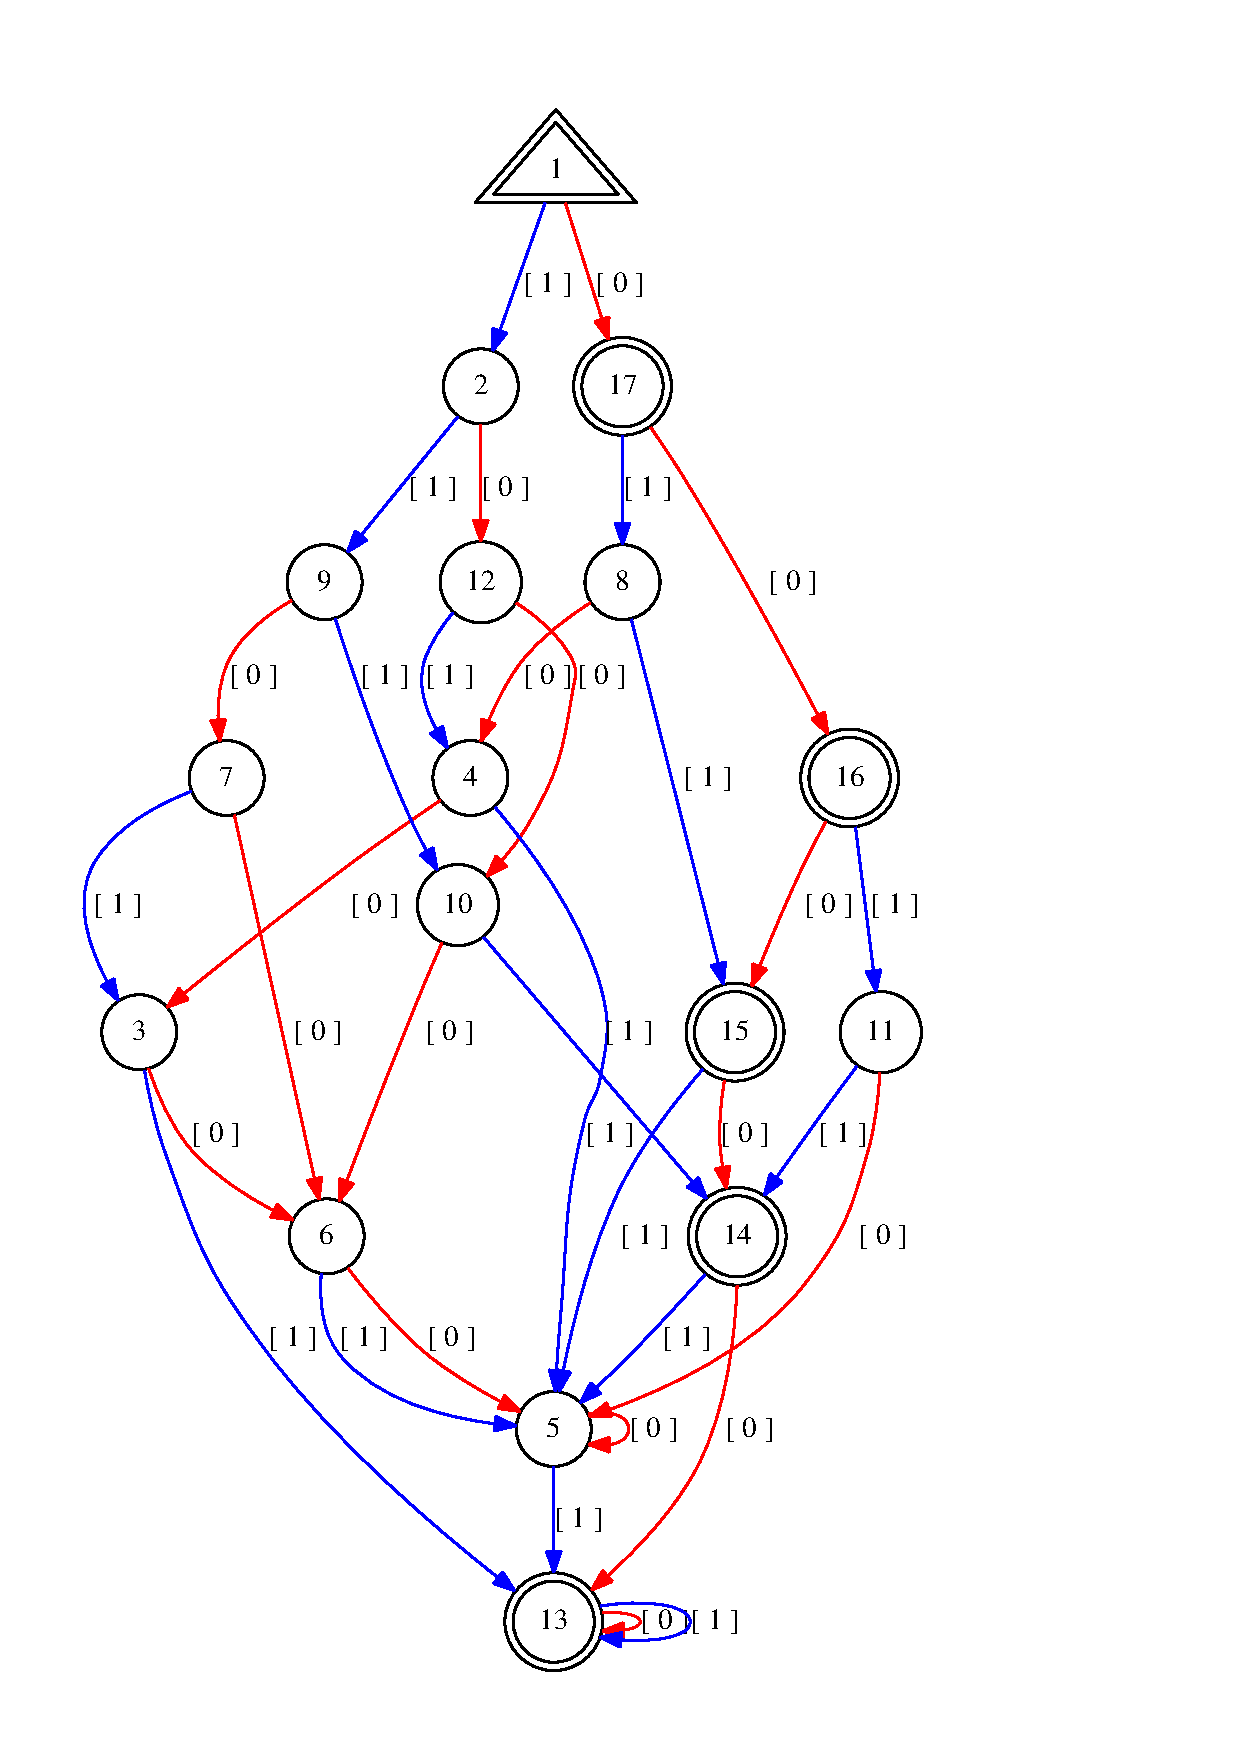
\includegraphics[width=0.4\textwidth]{img/aut1.jpg}
	\caption{A minimal DFA recognizing the numbers which can be purchased by the formula of \texttt{A}.}
	\label{aut1}
\end{figure}
  }

  
\chapter{\textcolor{Chapter }{Creating Predicata}}\label{Functions}
\logpage{[ 2, 0, 0 ]}
\hyperdef{L}{X7A3C47A378964F1F}{}
{
 
\section{\textcolor{Chapter }{Predicaton {\textendash} an extended finite automaton}}\logpage{[ 2, 1, 0 ]}
\hyperdef{L}{X7D04FF187F27BB76}{}
{
 

\subsection{\textcolor{Chapter }{Predicaton (Automaton with variable position list)}}
\logpage{[ 2, 1, 1 ]}\nobreak
\hyperdef{L}{X7FD70C2980210882}{}
{\noindent\textcolor{FuncColor}{$\triangleright$\enspace\texttt{Predicaton({\mdseries\slshape Automaton, VariablePositionList})\index{Predicaton@\texttt{Predicaton}!Automaton with variable position list}
\label{Predicaton:Automaton with variable position list}
}\hfill{\scriptsize (function)}}\\


 A \texttt{Predicaton} represents a first-order formulas, with $n$ free variables, containing the nullary operations $0$ and $1$ and the binary operation $+$. It consists of an \texttt{Automaton} and a \texttt{VariablePositionList}. 

 The first parameter is an \mbox{\texttt{\mdseries\slshape Automaton}} from the package \textsf{Automata}, which is created as follows: \texttt{Automaton(Type, Size, Alphabet, TransitionTable, Initial, Final)}. In order to create a \texttt{Predicaton} the \mbox{\texttt{\mdseries\slshape Type}} must either be \texttt{"det"} or \texttt{"nondet"}. The \mbox{\texttt{\mdseries\slshape Size}} is a positive integer giving the number of states. The \mbox{\texttt{\mdseries\slshape Alphabet}} must be a list of length $2^n$, i.e. the list of all n-tuples $\{0,1\}^n$. The \mbox{\texttt{\mdseries\slshape TransitionTable}} gives the transition matrix, where the entry at $(i,j)$ denotes the state reached with the $i$-th letter ($i$-th row) and the $j$-th state ($j$-th column). The \mbox{\texttt{\mdseries\slshape Initial}} and \mbox{\texttt{\mdseries\slshape Final}} are the initial and final state sets. 

 The second parameter \mbox{\texttt{\mdseries\slshape VariablePositionList}} must be of length $n$ and must contain $n$ pairwise distinct positive integers. It internally represents the occurring
variables in the first-order formula by assigning pairwise distinct natural
numbers to each free variable. The \mbox{\texttt{\mdseries\slshape VariablePositionList}} coincides with the letters, i.e. the $i$-th position in the $n$-tuples correspond to the variable position at the $i$-th position in the list. 

 A word over the alphabet $\{0,1\}^n$ can be turned into $n$ reversed binary representations of natural numbers by extracting the
components of the letters. The $i$-th row of a word (choosing the $i$-th component of each letter) corresponds to the $i$-th entry in the \mbox{\texttt{\mdseries\slshape VariablePositionList}}. The accepted words of the automaton represent those $n$ natural numbers, such that upon interpretation the first-order formula is
satisfied. 

 In the following example the \texttt{Automaton A} represents the formula $x+y=z$ with the following variables: the variable $x$ is assigned to $1$, the variable $y$ is assigned to $2 $ and the variable $z$ is assigned to $3$ The \texttt{Predicaton P} is created with the deterministic finite automaton \texttt{A} and the variable position list \texttt{[ 1, 2, 3 ]}. This means the first entry in the letters corresponds to the variable with
the assigned natural number 1, i.e. $x$, the second entry to the number $2$, i.e. the variable $y$ and the third entry to the number $3$, i.e. the variable $z$. 

 Later also a mathematically more intuitive method is introduced, see \texttt{Predicaton} (\ref{Predicaton:PredicataFormula}) for creating a \texttt{Predicaton} from a first-order formula. 
\begin{Verbatim}[commandchars=!@|,fontsize=\small,frame=single,label=Example]
  !gapprompt@gap>| !gapinput@A:=Automaton("det", 3,|
  !gapprompt@>| !gapinput@[ [ 0, 0, 0 ], [ 1, 0, 0 ], [ 0, 1, 0 ], [ 1, 1, 0 ],|
  !gapprompt@>| !gapinput@[ 0, 0, 1 ], [ 1, 0, 1 ], [ 0, 1, 1 ], [ 1, 1, 1 ] ],|
  !gapprompt@>| !gapinput@[ [ 1, 3, 3 ], [ 3, 2, 3 ], [ 3, 2, 3 ], [ 2, 3, 3 ],|
  !gapprompt@>| !gapinput@[ 3, 1, 3 ], [ 1, 3, 3 ], [ 1, 3, 3 ], [ 3, 2, 3 ] ],|
  !gapprompt@>| !gapinput@[ 1 ], [ 1 ]);|
  < deterministic automaton on 8 letters with 3 states >
  !gapprompt@gap>| !gapinput@P:=Predicaton( A, [ 1, 2, 3 ]);|
  < Predicaton: deterministic finite automaton on 8 letters with 3 states 
  and the variable position list [ 1, 2, 3 ]. >
\end{Verbatim}
 }

 

\subsection{\textcolor{Chapter }{BuildPredicaton}}
\logpage{[ 2, 1, 2 ]}\nobreak
\hyperdef{L}{X85732CF382B64BB8}{}
{\noindent\textcolor{FuncColor}{$\triangleright$\enspace\texttt{BuildPredicaton({\mdseries\slshape Type, Size, Alphabet, TransitionTable, Initial, Final, VariablePositionList})\index{BuildPredicaton@\texttt{BuildPredicaton}}
\label{BuildPredicaton}
}\hfill{\scriptsize (function)}}\\


 The function \texttt{BuildPredicaton} allows the creation of a \texttt{Predicaton} without specifying an \texttt{Automaton}. 
\begin{Verbatim}[commandchars=!@A,fontsize=\small,frame=single,label=Example]
  !gapprompt@gap>A !gapinput@P:=BuildPredicaton("det", 3, [ [ 0, 0, 0 ], [ 1, 0, 0 ], [ 0, 1, 0 ],A
  !gapprompt@>A !gapinput@[ 1, 1, 0 ], [ 0, 0, 1 ], [ 1, 0, 1 ], [ 0, 1, 1 ], [ 1, 1, 1 ] ],A
  !gapprompt@>A !gapinput@[ [ 1, 3, 3 ], [ 3, 2, 3 ], [ 3, 2, 3 ], [ 2, 3, 3 ], [ 3, 1, 3 ],A
  !gapprompt@>A !gapinput@[ 1, 3, 3 ], [ 1, 3, 3 ], [ 3, 2, 3 ] ], [ 1 ], [ 1 ], [ 1, 2, 3 ]);A
  < Predicaton: deterministic finite automaton on 8 letters with 3 states 
  and the variable position list [ 1, 2, 3 ]. >
  !gapprompt@gap>A !gapinput@Display(P);A
  Predicaton: deterministic finite automaton on 8 letters with 3 states, 
  the variable position list [ 1, 2, 3 ] and the following transitions:
                 |  1  2  3  
  ---------------------------
    [ 0, 0, 0 ]  |  1  3  3  
    [ 1, 0, 0 ]  |  3  2  3  
    [ 0, 1, 0 ]  |  3  2  3  
    [ 1, 1, 0 ]  |  2  3  3  
    [ 0, 0, 1 ]  |  3  1  3  
    [ 1, 0, 1 ]  |  1  3  3  
    [ 0, 1, 1 ]  |  1  3  3  
    [ 1, 1, 1 ]  |  3  2  3  
   Initial states: [ 1 ]
   Final states:   [ 1 ]
\end{Verbatim}
 }

 

\subsection{\textcolor{Chapter }{IsPredicaton}}
\logpage{[ 2, 1, 3 ]}\nobreak
\hyperdef{L}{X825D25A87C0D02DA}{}
{\noindent\textcolor{FuncColor}{$\triangleright$\enspace\texttt{IsPredicaton({\mdseries\slshape P})\index{IsPredicaton@\texttt{IsPredicaton}}
\label{IsPredicaton}
}\hfill{\scriptsize (function)}}\\


 The function \texttt{IsPredicaton} checks if \mbox{\texttt{\mdseries\slshape P}} is a \texttt{Predicaton}. 
\begin{Verbatim}[commandchars=!@|,fontsize=\small,frame=single,label=Example]
  !gapprompt@gap>| !gapinput@P:=BuildPredicaton("det", 2, [ [ 0, 0 ], [ 1, 0 ], [ 0, 1 ], [ 1, 1 ] ],|
  !gapprompt@>| !gapinput@[ [ 1, 2 ], [ 2, 2 ], [ 2, 2 ], [ 1, 2 ] ], [ 1 ], [ 1 ], [ 1, 2 ]);|
  < Predicaton: deterministic finite automaton on 4 letters with 2 states 
  and the variable position list [ 1, 2 ]. >
  !gapprompt@gap>| !gapinput@IsPredicaton(P);|
  true
\end{Verbatim}
 }

 

\subsection{\textcolor{Chapter }{Display (Predicaton)}}
\logpage{[ 2, 1, 4 ]}\nobreak
\hyperdef{L}{X818ADFEE7EC52BAF}{}
{\noindent\textcolor{FuncColor}{$\triangleright$\enspace\texttt{Display({\mdseries\slshape P})\index{Display@\texttt{Display}!Predicaton}
\label{Display:Predicaton}
}\hfill{\scriptsize (method)}}\\


 The method \texttt{Display} prints the transition table of the \texttt{Predicaton} \mbox{\texttt{\mdseries\slshape P}}. The left side are the letters of the alphabet, the top row are the states
and the transition from the $i$-th letter (row) and $j$-th state (column) is the entry $(i,j)$. 
\begin{Verbatim}[commandchars=!@B,fontsize=\small,frame=single,label=Example]
  !gapprompt@gap>B !gapinput@P:=Predicaton(Automaton("det", 3, [ [ 0, 0, 0 ], [ 1, 0, 0 ], [ 0, 1, 0 ],B
  !gapprompt@>B !gapinput@[ 1, 1, 0 ], [ 0, 0, 1 ], [ 1, 0, 1 ], [ 0, 1, 1 ], [ 1, 1, 1 ] ],B
  !gapprompt@>B !gapinput@[ [ 1, 3, 3 ], [ 3, 2, 3 ], [ 3, 2, 3 ], [ 2, 3, 3 ], [ 3, 1, 3 ],B
  !gapprompt@>B !gapinput@[ 1, 3, 3 ], [ 1, 3, 3 ], [ 3, 2, 3 ] ], [ 1 ], [ 1 ]), [ 1, 2, 3 ]);B
  < Predicaton: deterministic finite automaton on 8 letters with 3 states 
  and the variable position list [ 1, 2, 3 ]. >
  !gapprompt@gap>B !gapinput@Display(P);B
  Predicaton: deterministic finite automaton on 8 letters with 3 states, 
  the variable position list [ 1, 2, 3 ] and the following transitions:
                 |  1  2  3  
  ---------------------------
    [ 0, 0, 0 ]  |  1  3  3  
    [ 1, 0, 0 ]  |  3  2  3  
    [ 0, 1, 0 ]  |  3  2  3  
    [ 1, 1, 0 ]  |  2  3  3  
    [ 0, 0, 1 ]  |  3  1  3  
    [ 1, 0, 1 ]  |  1  3  3  
    [ 0, 1, 1 ]  |  1  3  3  
    [ 1, 1, 1 ]  |  3  2  3  
   Initial states: [ 1 ]
   Final states:   [ 1 ]
\end{Verbatim}
 }

 

\subsection{\textcolor{Chapter }{View (Predicaton)}}
\logpage{[ 2, 1, 5 ]}\nobreak
\hyperdef{L}{X854CA0237F4B8E5D}{}
{\noindent\textcolor{FuncColor}{$\triangleright$\enspace\texttt{View({\mdseries\slshape P})\index{View@\texttt{View}!Predicaton}
\label{View:Predicaton}
}\hfill{\scriptsize (method)}}\\


 The method \texttt{View} applied on a \texttt{Predicaton} \mbox{\texttt{\mdseries\slshape P}} returns the object text. 
\begin{Verbatim}[commandchars=!@|,fontsize=\small,frame=single,label=Example]
  !gapprompt@gap>| !gapinput@P:=Predicaton(Automaton("det", 3, [ [ 0 ], [ 1 ] ], [ [ 2, 2, 3 ],|
  !gapprompt@>| !gapinput@[ 3, 2, 2 ] ], [ 1 ], [ 3 ]), [ 1 ]);;|
  !gapprompt@gap>| !gapinput@View(P);|
  < Predicaton: deterministic finite automaton on 2 letters with 3 states 
  and the variable position list [ 1 ]. >
\end{Verbatim}
 }

 

\subsection{\textcolor{Chapter }{Print (Predicaton)}}
\logpage{[ 2, 1, 6 ]}\nobreak
\hyperdef{L}{X7C64F1F682B596FF}{}
{\noindent\textcolor{FuncColor}{$\triangleright$\enspace\texttt{Print({\mdseries\slshape P})\index{Print@\texttt{Print}!Predicaton}
\label{Print:Predicaton}
}\hfill{\scriptsize (method)}}\\


 The method \texttt{Print} applied on a \texttt{Predicaton} \mbox{\texttt{\mdseries\slshape P}} prints the input as a string. 
\begin{Verbatim}[commandchars=!@|,fontsize=\small,frame=single,label=Example]
  !gapprompt@gap>| !gapinput@P:=Predicaton(Automaton("det", 3, [ [ 0, 0 ], [ 1, 0 ], [ 0, 1 ], [ 1, 1 ] ], |
  !gapprompt@>| !gapinput@[ [ 1, 3, 3 ], [ 2, 3, 3 ], [ 3, 1, 3 ], [ 3, 2, 3 ] ], [ 1 ], [ 1 ]), |
  !gapprompt@>| !gapinput@[ 1, 2 ]);;|
  !gapprompt@gap>| !gapinput@Print(P);|
  Predicaton(Automaton("det", 3, [ [ 0, 0 ], [ 1, 0 ], [ 0, 1 ], [ 1, 1 ] ], [ [ \
  1, 3, 3 ], [ 2, 3, 3 ], [ 3, 1, 3 ], [ 3, 2, 3 ] ], [ 1 ], [ 1 ]), [ 1, 2 ]);;
  !gapprompt@gap>| !gapinput@String(P);|
  "Predicaton(Automaton(\"det\", 3, [ [ 0, 0 ], [ 1, 0 ], [ 0, 1 ], [ 1, 1 ] ], [ [\
  1, 3, 3 ], [ 2, 3, 3 ], [ 3, 1, 3 ], [ 3, 2, 3 ] ], [ 1 ], [ 1 ]), [ 1, 2 ]);;"
\end{Verbatim}
 }

 

\subsection{\textcolor{Chapter }{GetAlphabet}}
\logpage{[ 2, 1, 7 ]}\nobreak
\hyperdef{L}{X82BDA2E785ECEAB8}{}
{\noindent\textcolor{FuncColor}{$\triangleright$\enspace\texttt{GetAlphabet({\mdseries\slshape n})\index{GetAlphabet@\texttt{GetAlphabet}}
\label{GetAlphabet}
}\hfill{\scriptsize (function)}}\\


 The function \texttt{GetAlphabet} returns the alphabet $A^n$ for $A:=\{0,1\}$. 
\begin{Verbatim}[commandchars=!@B,fontsize=\small,frame=single,label=Example]
  !gapprompt@gap>B !gapinput@a1:=GetAlphabet(3);B
  [ [ 0, 0, 0 ], [ 1, 0, 0 ], [ 0, 1, 0 ], [ 1, 1, 0 ], 
    [ 0, 0, 1 ], [ 1, 0, 1 ], [ 0, 1, 1 ], [ 1, 1, 1 ] ]
  !gapprompt@gap>B !gapinput@P1:=Predicaton(Automaton("det", 3, a1,B
  !gapprompt@>B !gapinput@[ [ 1, 3, 3 ], [ 3, 2, 3 ], [ 3, 2, 3 ], [ 2, 3, 3 ], [ 3, 1, 3 ],B
  !gapprompt@>B !gapinput@[ 1, 3, 3 ], [ 1, 3, 3 ], [ 3, 2, 3 ] ], [ 1 ], [ 1 ]), [ 1, 2, 3 ]);;B
  !gapprompt@gap>B !gapinput@Display(P1);B
  Predicaton: deterministic finite automaton on 8 letters with 3 states, 
  the variable position list [ 1, 2, 3 ] and the following transitions:
                 |  1  2  3  
  ---------------------------
    [ 0, 0, 0 ]  |  1  3  3  
    [ 1, 0, 0 ]  |  3  2  3  
    [ 0, 1, 0 ]  |  3  2  3  
    [ 1, 1, 0 ]  |  2  3  3  
    [ 0, 0, 1 ]  |  3  1  3  
    [ 1, 0, 1 ]  |  1  3  3  
    [ 0, 1, 1 ]  |  1  3  3  
    [ 1, 1, 1 ]  |  3  2  3  
   Initial states: [ 1 ]
   Final states:   [ 1 ]
  !gapprompt@gap>B !gapinput@a2:=GetAlphabet(0);B
  [ [  ] ]
  !gapprompt@gap>B !gapinput@P2:=Predicaton(Automaton("det", 1, a2, [ [ 1 ] ], [ 1 ], [ 1 ]), [ ]);;B
  !gapprompt@gap>B !gapinput@Display(P2);B
  Predicaton: deterministic finite automaton on 1 letter with 1 state, 
  the variable position list [ ] and the following transitions:
         |  1  
  -------------
    [ ]  |  1  
   Initial states: [ 1 ]
   Final states:   [ 1 ]
\end{Verbatim}
 }

 }

 
\section{\textcolor{Chapter }{Basic functions on Automata and Predicata}}\label{Functions on Automata and Predicata}
\logpage{[ 2, 2, 0 ]}
\hyperdef{L}{X87ACF62385B06FFF}{}
{
 The package \textsf{Automata} allows lists of lists as input for the alphabet, but unfortunately is lacking
in further support. The functions regarding the alphabet takes only \texttt{ShallowCopy} whereas a list of lists \texttt{StructuralCopy} is needed, as well as the method \texttt{Display} for automata prints with some weird spacing. Therefore this package
reintroduces the basic \textsf{Automata} functions with another name to ensure full control. Nevertheless all credit
belongs to the creators of the package \textsf{Automata}. 

 Note that the \texttt{Predicata} in the following examples corresponds to first-order formulas. The accepted
natural numbers can be displayed with the functions from section \ref{Functions On Predicata}. 

 Furthermore, note that the following functions can be either called with an \texttt{Automaton} or a \texttt{Predicaton}. 

\subsection{\textcolor{Chapter }{DisplayAut}}
\logpage{[ 2, 2, 1 ]}\nobreak
\hyperdef{L}{X8720D1F186935FED}{}
{\noindent\textcolor{FuncColor}{$\triangleright$\enspace\texttt{DisplayAut({\mdseries\slshape P})\index{DisplayAut@\texttt{DisplayAut}}
\label{DisplayAut}
}\hfill{\scriptsize (function)}}\\


 The function \texttt{DisplayAut} prints the \texttt{Automaton} or \texttt{Predicaton} \mbox{\texttt{\mdseries\slshape P}} (called by \texttt{Display} (\ref{Display:Predicaton})). 
\begin{Verbatim}[commandchars=!@B,fontsize=\small,frame=single,label=Example]
  !gapprompt@gap>B !gapinput@A:=Automaton("det", 4, [ [ 0, 0 ], [ 1, 0 ], [ 0, 1 ], [ 1, 1 ] ],B
  !gapprompt@>B !gapinput@[ [ 3, 2, 2, 4 ], [ 2, 2, 4, 2 ], [ 2, 2, 3, 2 ], [ 3, 2, 2, 4 ] ],B
  !gapprompt@>B !gapinput@[ 1 ], [ 4 ]);B
  < deterministic automaton on 4 letters with 4 states >
  !gapprompt@gap>B !gapinput@DisplayAut(A);B
  deterministic finite automaton on 4 letters with 4 states 
  and the following transitions:
              |  1  2  3  4  
  ---------------------------
    [ 0, 0 ]  |  3  2  2  4  
    [ 1, 0 ]  |  2  2  4  2  
    [ 0, 1 ]  |  2  2  3  2  
    [ 1, 1 ]  |  3  2  2  4  
   Initial states: [ 1 ]
   Final states:   [ 4 ]
\end{Verbatim}
 }

 

\subsection{\textcolor{Chapter }{DrawPredicaton}}
\logpage{[ 2, 2, 2 ]}\nobreak
\hyperdef{L}{X81C510B7859139D9}{}
{\noindent\textcolor{FuncColor}{$\triangleright$\enspace\texttt{DrawPredicaton({\mdseries\slshape P})\index{DrawPredicaton@\texttt{DrawPredicaton}}
\label{DrawPredicaton}
}\hfill{\scriptsize (function)}}\\


 The function \texttt{DrawPredicaton} calls the function \texttt{DrawAutomaton} from the package \textsf{Automata} which uses \texttt{graphviz} \cite{KoutsofiosNorth:2002}, a software for drawing graphs developed at AT 
      \&
      T Labs, that can be obtained at \href{http://www.graphviz.org/} {\texttt{http://www.graphviz.org/}}. For further details please refer to the manual of the package \textsf{Automata}. 
\begin{Verbatim}[commandchars=!@B,fontsize=\small,frame=single,label=Example]
  !gapprompt@gap>B !gapinput@A:=Automaton("det", 4, [ [ 0, 0 ], [ 1, 0 ], [ 0, 1 ], [ 1, 1 ] ],B
  !gapprompt@>B !gapinput@[ [ 3, 2, 2, 4 ], [ 2, 2, 4, 2 ], [ 2, 2, 3, 2 ], [ 3, 2, 2, 4 ] ],B
  !gapprompt@>B !gapinput@[ 1 ], [ 4 ]);B
  < deterministic automaton on 4 letters with 4 states >
  !gapprompt@gap>B !gapinput@DisplayAut(A);B
  deterministic finite automaton on 4 letters with 4 states 
  and the following transitions:
              |  1  2  3  4  
  ---------------------------
    [ 0, 0 ]  |  3  2  2  4  
    [ 1, 0 ]  |  2  2  4  2  
    [ 0, 1 ]  |  2  2  3  2  
    [ 1, 1 ]  |  3  2  2  4  
   Initial states: [ 1 ]
   Final states:   [ 4 ]
\end{Verbatim}
 }

 

\subsection{\textcolor{Chapter }{IsDeterministicAut}}
\logpage{[ 2, 2, 3 ]}\nobreak
\hyperdef{L}{X837962738642AA13}{}
{\noindent\textcolor{FuncColor}{$\triangleright$\enspace\texttt{IsDeterministicAut({\mdseries\slshape P})\index{IsDeterministicAut@\texttt{IsDeterministicAut}}
\label{IsDeterministicAut}
}\hfill{\scriptsize (function)}}\\


 The function \texttt{IsDeterministicAut} checks if the \texttt{Type} of an \texttt{Automaton} or a \texttt{Predicaton} \mbox{\texttt{\mdseries\slshape P}} is \texttt{"det"}. If yes then \texttt{true}, otherwise \texttt{false}. 
\begin{Verbatim}[commandchars=!@|,fontsize=\small,frame=single,label=Example]
  !gapprompt@gap>| !gapinput@P:=Predicaton(Automaton("det", 5, [ [ 0 ], [ 1 ] ], [ [ 1, 2, 2, 3, 2 ], |
  !gapprompt@>| !gapinput@[ 2, 2, 1, 2, 4 ] ], [ 5 ], [ 1 ]), [ 1 ]);|
  < Predicaton: deterministic finite automaton on 2 letters with 5 states 
  and the variable position list [ 1 ]. >
  !gapprompt@gap>| !gapinput@IsDeterministicAut(P);|
  true
\end{Verbatim}
 }

 

\subsection{\textcolor{Chapter }{IsNonDeterministicAut}}
\logpage{[ 2, 2, 4 ]}\nobreak
\hyperdef{L}{X82BB21D07836FC43}{}
{\noindent\textcolor{FuncColor}{$\triangleright$\enspace\texttt{IsNonDeterministicAut({\mdseries\slshape P})\index{IsNonDeterministicAut@\texttt{IsNonDeterministicAut}}
\label{IsNonDeterministicAut}
}\hfill{\scriptsize (function)}}\\


 The function \texttt{IsNonDeterministicAut} checks if the \texttt{Type} of an \texttt{Automaton} or a \texttt{Predicaton} \mbox{\texttt{\mdseries\slshape P}} is \texttt{"nondet"}. If yes then \texttt{true}, otherwise \texttt{false}. 
\begin{Verbatim}[commandchars=!@B,fontsize=\small,frame=single,label=Example]
  !gapprompt@gap>B !gapinput@P:=Predicaton(Automaton("nondet", 2, [ [ 0 ], [ 1 ] ], [ [ 1  ], [  ] ],B
  !gapprompt@>B !gapinput@[ 1 ], [ 1 ]), [ 1 ]);B
  < Predicaton: nondeterministic finite automaton on 2 letters with 2 states 
  and the variable position list [ 1 ]. >
  !gapprompt@gap>B !gapinput@Display(P);B
  Predicaton: nondeterministic finite automaton on 2 letters with 2 states, 
  the variable position list [ 1 ] and the following transitions:
           |  1      2      
  --------------------------
    [ 0 ]  |  [ 1 ]  [ ]    
    [ 1 ]  |  [ ]    [ ]    
   Initial states: [ 1 ]
   Final states:   [ 1 ]
  !gapprompt@gap>B !gapinput@IsNonDeterministicAut(P);B
  true
\end{Verbatim}
 }

 

\subsection{\textcolor{Chapter }{TypeOfAut}}
\logpage{[ 2, 2, 5 ]}\nobreak
\hyperdef{L}{X8291B3E379A6DE70}{}
{\noindent\textcolor{FuncColor}{$\triangleright$\enspace\texttt{TypeOfAut({\mdseries\slshape P})\index{TypeOfAut@\texttt{TypeOfAut}}
\label{TypeOfAut}
}\hfill{\scriptsize (function)}}\\


 The function \texttt{TypeOfAut} returns the \texttt{Type} of an \texttt{Automaton} or a \texttt{Predicaton} \mbox{\texttt{\mdseries\slshape P}}, either \texttt{"det"}, \texttt{"nondet"} or \texttt{"epsilon"}. Note that a \texttt{Predicaton} can only be a deterministic or nondeterministic finite automaton. 
\begin{Verbatim}[commandchars=!@|,fontsize=\small,frame=single,label=Example]
  !gapprompt@gap>| !gapinput@P:=Predicaton(Automaton("det", 5, [ [ 0, 0 ], [ 1, 0 ], [ 0, 1 ], [ 1, 1 ] ], |
  !gapprompt@>| !gapinput@[ [ 2, 2, 2, 2, 5 ], [ 2, 2, 5, 2, 2 ], [ 2, 2, 2, 3, 2 ], [ 4, 2, 2, 2, 2 ] ],|
  !gapprompt@>| !gapinput@[ 1 ], [ 5 ]), [ 1, 2 ]);;|
  !gapprompt@gap>| !gapinput@TypeOfAut(P);|
  "det"
\end{Verbatim}
 }

 

\subsection{\textcolor{Chapter }{AlphabetOfAut}}
\logpage{[ 2, 2, 6 ]}\nobreak
\hyperdef{L}{X79387C217C9E0645}{}
{\noindent\textcolor{FuncColor}{$\triangleright$\enspace\texttt{AlphabetOfAut({\mdseries\slshape P})\index{AlphabetOfAut@\texttt{AlphabetOfAut}}
\label{AlphabetOfAut}
}\hfill{\scriptsize (function)}}\\


 The function \texttt{AlphabetOfAut} returns the size of an \texttt{Alphabet} of an \texttt{Automaton} or a \texttt{Predicaton} \mbox{\texttt{\mdseries\slshape P}}. 
\begin{Verbatim}[commandchars=!@|,fontsize=\small,frame=single,label=Example]
  !gapprompt@gap>| !gapinput@P:=Predicaton(Automaton("det", 2, [ [ 0, 0 ], [ 1, 0 ], [ 0, 1 ], [ 1, 1 ] ], |
  !gapprompt@>| !gapinput@[ [ 1, 2 ], [ 2, 2 ], [ 2, 2 ], [ 1, 2 ] ], [ 1 ], [ 1 ]), [ 1, 2 ]);;|
  !gapprompt@gap>| !gapinput@AlphabetOfAut(P);|
  4
\end{Verbatim}
 }

 

\subsection{\textcolor{Chapter }{AlphabetOfAutAsList}}
\logpage{[ 2, 2, 7 ]}\nobreak
\hyperdef{L}{X7BB104337B972500}{}
{\noindent\textcolor{FuncColor}{$\triangleright$\enspace\texttt{AlphabetOfAutAsList({\mdseries\slshape P})\index{AlphabetOfAutAsList@\texttt{AlphabetOfAutAsList}}
\label{AlphabetOfAutAsList}
}\hfill{\scriptsize (function)}}\\


 The function \texttt{AlphabetOfAutAsList} returns a \texttt{StructuralCopy} of the \texttt{Alphabet} of an \texttt{Automaton} or a \texttt{Predicaton} \mbox{\texttt{\mdseries\slshape P}}. 
\begin{Verbatim}[commandchars=!@|,fontsize=\small,frame=single,label=Example]
  !gapprompt@gap>| !gapinput@# Continued |
  !gapprompt@gap>| !gapinput@AlphabetOfAutAsList(P);|
  [ [ 0, 0 ], [ 1, 0 ], [ 0, 1 ], [ 1, 1 ] ]
\end{Verbatim}
 }

 

\subsection{\textcolor{Chapter }{NumberStatesOfAut}}
\logpage{[ 2, 2, 8 ]}\nobreak
\hyperdef{L}{X7A1F901B7C19CB01}{}
{\noindent\textcolor{FuncColor}{$\triangleright$\enspace\texttt{NumberStatesOfAut({\mdseries\slshape P})\index{NumberStatesOfAut@\texttt{NumberStatesOfAut}}
\label{NumberStatesOfAut}
}\hfill{\scriptsize (function)}}\\


 The function \texttt{NumberStatesOfAut} returns the number of the \texttt{States} of an \texttt{Automaton} or a \texttt{Predicaton} \mbox{\texttt{\mdseries\slshape P}}. 
\begin{Verbatim}[commandchars=!@|,fontsize=\small,frame=single,label=Example]
  !gapprompt@gap>| !gapinput@P:=Predicaton(Automaton("det", 5, [ [ 0, 0 ], [ 1, 0 ], [ 0, 1 ], [ 1, 1 ] ],|
  !gapprompt@>| !gapinput@[ [ 2, 2, 2, 2, 5 ], [ 4, 2, 5, 3, 2 ], [ 4, 2, 5, 3, 2 ], [ 2, 2, 2, 2, 2 ] ], |
  !gapprompt@>| !gapinput@[ 1 ], [ 5 ]), [ 1, 2 ]);;|
  !gapprompt@gap>| !gapinput@NumberStatesOfAut(P);|
  5
\end{Verbatim}
 }

 

\subsection{\textcolor{Chapter }{SortedStatesAut}}
\logpage{[ 2, 2, 9 ]}\nobreak
\hyperdef{L}{X7C0D702D869F7E62}{}
{\noindent\textcolor{FuncColor}{$\triangleright$\enspace\texttt{SortedStatesAut({\mdseries\slshape P})\index{SortedStatesAut@\texttt{SortedStatesAut}}
\label{SortedStatesAut}
}\hfill{\scriptsize (function)}}\\


 The function \texttt{SortedStatesAut} returns the \texttt{Automaton} or the \texttt{Predicaton} \mbox{\texttt{\mdseries\slshape P}} with sorted \texttt{States}, such that the initial states have the lowest and the final states the
highest number. 
\begin{Verbatim}[commandchars=!@B,fontsize=\small,frame=single,label=Example]
  !gapprompt@gap>B !gapinput@P:=Predicaton(Automaton("det", 5, [ [ 0 ], [ 1 ] ], [ [ 1, 2, 2, 2, 2 ],B
  !gapprompt@>B !gapinput@[ 2, 2, 1, 3, 4 ] ], [ 5 ], [ 1 ]), [ 1 ]);;B
  !gapprompt@gap>B !gapinput@Display(P);B
  Predicaton: deterministic finite automaton on 2 letters with 5 states, 
  the variable position list [ 1 ] and the following transitions:
           |  1  2  3  4  5  
  ---------------------------
    [ 0 ]  |  1  2  2  2  2  
    [ 1 ]  |  2  2  1  3  4  
   Initial states: [ 5 ]
   Final states:   [ 1 ]
  !gapprompt@gap>B !gapinput@S:=SortedStatesAut(P);;B
  !gapprompt@gap>B !gapinput@Display(S);B
  Predicaton: deterministic finite automaton on 2 letters with 5 states, 
  the variable position list [ 1 ] and the following transitions:
           |  1  2  3  4  5  
  ---------------------------
    [ 0 ]  |  2  2  2  2  5  
    [ 1 ]  |  4  2  5  3  2  
   Initial states: [ 1 ]
   Final states:   [ 5 ]
\end{Verbatim}
 }

 

\subsection{\textcolor{Chapter }{TransitionMatrixOfAut}}
\logpage{[ 2, 2, 10 ]}\nobreak
\hyperdef{L}{X8150E8F278688F79}{}
{\noindent\textcolor{FuncColor}{$\triangleright$\enspace\texttt{TransitionMatrixOfAut({\mdseries\slshape P})\index{TransitionMatrixOfAut@\texttt{TransitionMatrixOfAut}}
\label{TransitionMatrixOfAut}
}\hfill{\scriptsize (function)}}\\


 The function \texttt{TransitionMatrixOfAut} returns a \texttt{StructuralCopy} of the \texttt{TransitionMatrix} of an \texttt{Automaton} or a \texttt{Predicaton} \mbox{\texttt{\mdseries\slshape P}}. 
\begin{Verbatim}[commandchars=!@B,fontsize=\small,frame=single,label=Example]
  !gapprompt@gap>B !gapinput@P:=Predicaton(Automaton("det", 5, [ [ 0 ], [ 1 ] ], [ [ 1, 2, 2, 2, 2 ],B
  !gapprompt@>B !gapinput@[ 2, 2, 1, 3, 4 ] ], [ 5 ], [ 1 ]), [ 1 ]);;B
  !gapprompt@gap>B !gapinput@Display(P);B
  Predicaton: deterministic finite automaton on 2 letters with 5 states, 
  the variable position list [ 1 ] and the following transitions:
           |  1  2  3  4  5  
  ---------------------------
    [ 0 ]  |  1  2  2  2  2  
    [ 1 ]  |  2  2  1  3  4  
   Initial states: [ 5 ]
   Final states:   [ 1 ]
  !gapprompt@gap>B !gapinput@TransitionMatrixOfAut(P);B
  [ [ 1, 2, 2, 2, 2 ], [ 2, 2, 1, 3, 4 ] ]
\end{Verbatim}
 }

 

\subsection{\textcolor{Chapter }{InitialStatesOfAut}}
\logpage{[ 2, 2, 11 ]}\nobreak
\hyperdef{L}{X785309187BAFF773}{}
{\noindent\textcolor{FuncColor}{$\triangleright$\enspace\texttt{InitialStatesOfAut({\mdseries\slshape P})\index{InitialStatesOfAut@\texttt{InitialStatesOfAut}}
\label{InitialStatesOfAut}
}\hfill{\scriptsize (function)}}\\


 The function \texttt{InitialStatesOfAut} returns the \texttt{Initial} states of an \texttt{Automaton} or a \texttt{Predicaton} \mbox{\texttt{\mdseries\slshape P}}. 
\begin{Verbatim}[commandchars=!@|,fontsize=\small,frame=single,label=Example]
  !gapprompt@gap>| !gapinput@P:=Predicaton(Automaton("det", 5, [ [ 0 ], [ 1 ] ], [ [ 2, 2, 2, 3, 5 ], |
  !gapprompt@>| !gapinput@[ 4, 2, 5, 2, 2 ] ], [ 1 ], [ 5 ]), [ 1 ]);;|
  !gapprompt@gap>| !gapinput@InitialStatesOfAut(P);|
  [ 1 ]
\end{Verbatim}
 }

 

\subsection{\textcolor{Chapter }{SetInitialStatesOfAut}}
\logpage{[ 2, 2, 12 ]}\nobreak
\hyperdef{L}{X812E72137E8ED4E1}{}
{\noindent\textcolor{FuncColor}{$\triangleright$\enspace\texttt{SetInitialStatesOfAut({\mdseries\slshape P})\index{SetInitialStatesOfAut@\texttt{SetInitialStatesOfAut}}
\label{SetInitialStatesOfAut}
}\hfill{\scriptsize (function)}}\\


 The function \texttt{SetInitialStatesOfAut} sets the \texttt{Initial} states of an \texttt{Automaton} or a \texttt{Predicaton} \mbox{\texttt{\mdseries\slshape P}}. 
\begin{Verbatim}[commandchars=!@B,fontsize=\small,frame=single,label=Example]
  !gapprompt@gap>B !gapinput@P:=Predicaton(Automaton("det", 5, [ [ 0 ], [ 1 ] ], [ [ 2, 2, 2, 3, 5 ],B
  !gapprompt@>B !gapinput@[ 4, 2, 5, 2, 2 ] ], [ 1 ], [ 5 ]), [ 1 ]);;B
  !gapprompt@gap>B !gapinput@Display(P);B
  Predicaton: deterministic finite automaton on 2 letters with 5 states, 
  the variable position list [ 1 ] and the following transitions:
           |  1  2  3  4  5  
  ---------------------------
    [ 0 ]  |  2  2  2  3  5  
    [ 1 ]  |  4  2  5  2  2  
   Initial states: [ 1 ]
   Final states:   [ 5 ]
  !gapprompt@gap>B !gapinput@SetInitialStatesOfAut(P, 3);B
  !gapprompt@gap>B !gapinput@Display(P);B
  Predicaton: deterministic finite automaton on 2 letters with 5 states, 
  the variable position list [ 1 ] and the following transitions:
           |  1  2  3  4  5  
  ---------------------------
    [ 0 ]  |  2  2  2  3  5  
    [ 1 ]  |  4  2  5  2  2  
   Initial states: [ 3 ]
   Final states:   [ 5 ]
\end{Verbatim}
 }

 

\subsection{\textcolor{Chapter }{FinalStatesOfAut}}
\logpage{[ 2, 2, 13 ]}\nobreak
\hyperdef{L}{X867925CC844D77D5}{}
{\noindent\textcolor{FuncColor}{$\triangleright$\enspace\texttt{FinalStatesOfAut({\mdseries\slshape P})\index{FinalStatesOfAut@\texttt{FinalStatesOfAut}}
\label{FinalStatesOfAut}
}\hfill{\scriptsize (function)}}\\


 The function \texttt{FinalStatesOfAut} returns the \texttt{Final} states of an \texttt{Automaton} or a \texttt{Predicaton} \mbox{\texttt{\mdseries\slshape P}}. 
\begin{Verbatim}[commandchars=!@B,fontsize=\small,frame=single,label=Example]
  !gapprompt@gap>B !gapinput@P:=Predicaton(Automaton("det", 4, [ [ 0 ], [ 1 ] ], [ [ 2, 2, 2, 4 ],B
  !gapprompt@>B !gapinput@[ 3, 2, 4, 2 ] ], [ 1 ], [ 4 ]), [ 1 ]);;B
  !gapprompt@gap>B !gapinput@Display(P);B
  Predicaton: deterministic finite automaton on 2 letters with 4 states, 
  the variable position list [ 1 ] and the following transitions:
           |  1  2  3  4  
  ------------------------
    [ 0 ]  |  2  2  2  4  
    [ 1 ]  |  3  2  4  2  
   Initial states: [ 1 ]
   Final states:   [ 4 ]
  !gapprompt@gap>B !gapinput@FinalStatesOfAut(P);B
  [ 4 ]
\end{Verbatim}
 }

 

\subsection{\textcolor{Chapter }{SetFinalStatesOfAut}}
\logpage{[ 2, 2, 14 ]}\nobreak
\hyperdef{L}{X80EF044086173940}{}
{\noindent\textcolor{FuncColor}{$\triangleright$\enspace\texttt{SetFinalStatesOfAut({\mdseries\slshape P})\index{SetFinalStatesOfAut@\texttt{SetFinalStatesOfAut}}
\label{SetFinalStatesOfAut}
}\hfill{\scriptsize (function)}}\\


 The function \texttt{SetFinalStatesOfAut} sets the \texttt{Final} states of an \texttt{Automaton} or a \texttt{Predicaton} \mbox{\texttt{\mdseries\slshape P}}. 
\begin{Verbatim}[commandchars=!@B,fontsize=\small,frame=single,label=Example]
  !gapprompt@gap>B !gapinput@P:=Predicaton(Automaton("det", 4, [ [ 0 ], [ 1 ] ], [ [ 2, 2, 2, 4 ],B
  !gapprompt@>B !gapinput@[ 3, 2, 4, 2 ] ], [ 1 ], [ 4 ]), [ 1 ]);;B
  !gapprompt@gap>B !gapinput@Display(P);B
  Predicaton: deterministic finite automaton on 2 letters with 4 states, 
  the variable position list [ 1 ] and the following transitions:
           |  1  2  3  4  
  ------------------------
    [ 0 ]  |  2  2  2  4  
    [ 1 ]  |  3  2  4  2  
   Initial states: [ 1 ]
   Final states:   [ 4 ]
  !gapprompt@gap>B !gapinput@SetFinalStatesOfAut(P, [ 1, 2, 3 ]);B
  !gapprompt@gap>B !gapinput@Display(P);B
  Predicaton: deterministic finite automaton on 2 letters with 4 states, 
  the variable position list [ 1 ] and the following transitions:
           |  1  2  3  4  
  ------------------------
    [ 0 ]  |  2  2  2  4  
    [ 1 ]  |  3  2  4  2  
   Initial states: [ 1 ]
   Final states:   [ 1, 2, 3 ]
\end{Verbatim}
 }

 

\subsection{\textcolor{Chapter }{SinkStatesOfAut}}
\logpage{[ 2, 2, 15 ]}\nobreak
\hyperdef{L}{X84FC26AF7F7F8393}{}
{\noindent\textcolor{FuncColor}{$\triangleright$\enspace\texttt{SinkStatesOfAut({\mdseries\slshape P})\index{SinkStatesOfAut@\texttt{SinkStatesOfAut}}
\label{SinkStatesOfAut}
}\hfill{\scriptsize (function)}}\\


 The function \texttt{SinkStatesOfAut} returns the sink states of an \texttt{Automaton} or a \texttt{Predicaton} \mbox{\texttt{\mdseries\slshape P}}. 
\begin{Verbatim}[commandchars=!@B,fontsize=\small,frame=single,label=Example]
  !gapprompt@gap>B !gapinput@P:=Predicaton(Automaton("det", 3, [ [ 0 ], [ 1 ] ], [ [ 2, 2, 3 ],B
  !gapprompt@>B !gapinput@[ 3, 2, 2 ] ], [ 1 ], [ 3 ]), [ 1 ]);;B
  !gapprompt@gap>B !gapinput@Display(P);B
  Predicaton: deterministic finite automaton on 2 letters with 3 states, 
  the variable position list [ 1 ] and the following transitions:
           |  1  2  3  
  ---------------------
    [ 0 ]  |  2  2  3  
    [ 1 ]  |  3  2  2  
   Initial states: [ 1 ]
   Final states:   [ 3 ]
  !gapprompt@gap>B !gapinput@SinkStatesOfAut(P);B
  [ 2 ]
\end{Verbatim}
 }

 

\subsection{\textcolor{Chapter }{PermutedStatesAut}}
\logpage{[ 2, 2, 16 ]}\nobreak
\hyperdef{L}{X82B09FBE86E7D43A}{}
{\noindent\textcolor{FuncColor}{$\triangleright$\enspace\texttt{PermutedStatesAut({\mdseries\slshape P, p})\index{PermutedStatesAut@\texttt{PermutedStatesAut}}
\label{PermutedStatesAut}
}\hfill{\scriptsize (function)}}\\


 The function \texttt{PermutedStatesAut} permutes the names of the states of an \texttt{Automaton} or a \texttt{Predicaton} \mbox{\texttt{\mdseries\slshape P}}. The list \mbox{\texttt{\mdseries\slshape p}} contains all states, where the state \texttt{i} (i.e. \texttt{i}-th position) is mapped to the state \texttt{p[i]}. 
\begin{Verbatim}[commandchars=!@B,fontsize=\small,frame=single,label=Example]
  !gapprompt@gap>B !gapinput@P:=Predicaton(Automaton("det", 6, [ [ 0 ], [ 1 ] ], [ [ 5, 2, 2, 3, 4, 6 ],B
  !gapprompt@>B !gapinput@[ 2, 2, 6, 2, 2, 2 ] ], [ 1 ], [ 6 ]), [ 1 ]);;B
  !gapprompt@gap>B !gapinput@Display(P);B
  Predicaton: deterministic finite automaton on 2 letters with 6 states, 
  the variable position list [ 1 ] and the following transitions:
           |  1  2  3  4  5  6  
  ------------------------------
    [ 0 ]  |  5  2  2  3  4  6  
    [ 1 ]  |  2  2  6  2  2  2  
   Initial states: [ 1 ]
   Final states:   [ 6 ]
  !gapprompt@gap>B !gapinput@Q:=PermutedStatesAut(P,[1,6,4,3,2,5]);;B
  !gapprompt@gap>B !gapinput@Display(Q);B
  Predicaton: deterministic finite automaton on 2 letters with 6 states, 
  the variable position list [ 1 ] and the following transitions:
           |  1  2  3  4  5  6  
  ------------------------------
    [ 0 ]  |  2  3  4  6  5  6  
    [ 1 ]  |  6  6  6  5  6  6  
   Initial states: [ 1 ]
   Final states:   [ 5 ]
\end{Verbatim}
 }

 

\subsection{\textcolor{Chapter }{CopyAut}}
\logpage{[ 2, 2, 17 ]}\nobreak
\hyperdef{L}{X84BCD89583863028}{}
{\noindent\textcolor{FuncColor}{$\triangleright$\enspace\texttt{CopyAut({\mdseries\slshape P})\index{CopyAut@\texttt{CopyAut}}
\label{CopyAut}
}\hfill{\scriptsize (function)}}\\
\noindent\textcolor{FuncColor}{$\triangleright$\enspace\texttt{CopyPredicaton({\mdseries\slshape P})\index{CopyPredicaton@\texttt{CopyPredicaton}}
\label{CopyPredicaton}
}\hfill{\scriptsize (function)}}\\


 The function \texttt{CopyAut} copies either the \texttt{Automaton} or the \texttt{Predicaton} \mbox{\texttt{\mdseries\slshape P}}. 
\begin{Verbatim}[commandchars=!@B,fontsize=\small,frame=single,label=Example]
  !gapprompt@gap>B !gapinput@P:=Predicaton(Automaton("det", 2, [ [ 0 ], [ 1 ] ], [ [ 1, 2 ], [ 2, 2 ] ],B
  !gapprompt@>B !gapinput@[ 1 ], [ 1 ]), [ 1 ]);;B
  !gapprompt@gap>B !gapinput@C:=CopyAut(P);;B
  !gapprompt@gap>B !gapinput@SetFinalStatesOfAut(C, 2);B
  !gapprompt@gap>B !gapinput@Display(P);B
  Predicaton: deterministic finite automaton on 2 letters with 2 states, 
  the variable position list [ 1 ] and the following transitions:
           |  1  2  
  ------------------
    [ 0 ]  |  1  2  
    [ 1 ]  |  2  2  
   Initial states: [ 1 ]
   Final states:   [ 1 ]
  !gapprompt@gap>B !gapinput@Display(C);B
  Predicaton: deterministic finite automaton on 2 letters with 2 states, 
  the variable position list [ 1 ] and the following transitions:
           |  1  2  
  ------------------
    [ 0 ]  |  1  2  
    [ 1 ]  |  2  2  
   Initial states: [ 1 ]
   Final states:   [ 2 ]
\end{Verbatim}
 }

 

\subsection{\textcolor{Chapter }{MinimalAut}}
\logpage{[ 2, 2, 18 ]}\nobreak
\hyperdef{L}{X8377BBD382180F49}{}
{\noindent\textcolor{FuncColor}{$\triangleright$\enspace\texttt{MinimalAut({\mdseries\slshape P})\index{MinimalAut@\texttt{MinimalAut}}
\label{MinimalAut}
}\hfill{\scriptsize (function)}}\\


 The function \texttt{MinimalAut} returns the minimal deterministic finite automaton of an \texttt{Automaton} \mbox{\texttt{\mdseries\slshape P}}. Given a \texttt{Predicaton} \mbox{\texttt{\mdseries\slshape P}} its automaton is minimized and returned as a \texttt{Predicaton} with the same variable position list. 
\begin{Verbatim}[commandchars=!@B,fontsize=\small,frame=single,label=Example]
  !gapprompt@gap>B !gapinput@P:=Predicaton(Automaton("det", 9, [ [ 0, 0 ], [ 1, 0 ], [ 0, 1 ], [ 1, 1 ] ],B
  !gapprompt@>B !gapinput@[ [ 2, 6, 7, 4, 5, 4, 5, 8, 9 ], [ 3, 6, 6, 4, 4, 4, 4, 8, 8 ],B
  !gapprompt@>B !gapinput@[ 4, 4, 5, 4, 5, 8, 9, 4, 5 ], [ 5, 4, 4, 4, 4, 8, 8, 4, 4 ] ],B
  !gapprompt@>B !gapinput@[ 1 ], [ 9 ]), [ 1, 2 ]);;B
  !gapprompt@gap>B !gapinput@Display(P);B
  Predicaton: deterministic finite automaton on 4 letters with 9 states, 
  the variable position list [ 1, 2 ] and the following transitions:
              |  1  2  3  4  5  6  7  8  9  
  ------------------------------------------
    [ 0, 0 ]  |  2  6  7  4  5  4  5  8  9  
    [ 1, 0 ]  |  3  6  6  4  4  4  4  8  8  
    [ 0, 1 ]  |  4  4  5  4  5  8  9  4  5  
    [ 1, 1 ]  |  5  4  4  4  4  8  8  4  4  
   Initial states: [ 1 ]
   Final states:   [ 9 ]
  !gapprompt@gap>B !gapinput@M:=MinimalAut(P);;B
  !gapprompt@gap>B !gapinput@Display(M);B
  Predicaton: deterministic finite automaton on 4 letters with 5 states, 
  the variable position list [ 1, 2 ] and the following transitions:
              |  1  2  3  4  5  
  ------------------------------
    [ 0, 0 ]  |  1  2  2  3  2  
    [ 1, 0 ]  |  2  2  2  2  4  
    [ 0, 1 ]  |  2  2  1  2  2  
    [ 1, 1 ]  |  2  2  2  2  2  
   Initial states: [ 5 ]
   Final states:   [ 1 ]
  !gapprompt@gap>B !gapinput@P:=Predicaton(Automaton("nondet", 8, [ [ 0 ], [ 1 ] ],B
  !gapprompt@>B !gapinput@[ [ [ 2 ], [ 2 ], [ 2 ], [ 4 ], [ 7 ], [ 6 ], [ 6 ], [ 8 ] ],B
  !gapprompt@>B !gapinput@[ [ 3 ], [ 2 ], [ 4 ], [ 2 ], [ 6 ], [ 6 ], [ 8 ], [ 6 ] ] ],B
  !gapprompt@>B !gapinput@[ 1, 5 ], [ 4, 8 ]), [ 1 ]);;B
  !gapprompt@gap>B !gapinput@M:=MinimalAut(P);;B
  !gapprompt@gap>B !gapinput@Display(M);B
  Predicaton: deterministic finite automaton on 2 letters with 4 states, 
  the variable position list [ 1 ] and the following transitions:
           |  1  2  3  4  
  ------------------------
    [ 0 ]  |  1  2  2  3  
    [ 1 ]  |  2  2  1  3  
   Initial states: [ 4 ]
   Final states:   [ 1 ]
\end{Verbatim}
 }

 

\subsection{\textcolor{Chapter }{NegatedAut}}
\logpage{[ 2, 2, 19 ]}\nobreak
\hyperdef{L}{X802357D181BD700C}{}
{\noindent\textcolor{FuncColor}{$\triangleright$\enspace\texttt{NegatedAut({\mdseries\slshape P})\index{NegatedAut@\texttt{NegatedAut}}
\label{NegatedAut}
}\hfill{\scriptsize (function)}}\\


 The function \texttt{NegatedAut} changes the \texttt{Final} states to non-final ones and the non-final states to \texttt{Final} ones. 
\begin{Verbatim}[commandchars=!@B,fontsize=\small,frame=single,label=Example]
  !gapprompt@gap>B !gapinput@P:=Predicaton(Automaton("det", 4, [ [ 0 ], [ 1 ] ], [ [ 2, 2, 2, 4 ],B
  !gapprompt@>B !gapinput@[ 3, 2, 4, 2 ] ], [ 1 ], [ 4 ]), [ 1 ]);;B
  !gapprompt@gap>B !gapinput@Display(P);B
  Predicaton: deterministic finite automaton on 2 letters with 4 states, 
  the variable position list [ 1 ] and the following transitions:
           |  1  2  3  4  
  ------------------------
    [ 0 ]  |  2  2  2  4  
    [ 1 ]  |  3  2  4  2  
   Initial states: [ 1 ]
   Final states:   [ 4 ]
  !gapprompt@gap>B !gapinput@Q:=NegatedAut(P);;B
  !gapprompt@gap>B !gapinput@Display(Q);B
  Predicaton: deterministic finite automaton on 2 letters with 4 states, 
  the variable position list [ 1 ] and the following transitions:
           |  1  2  3  4  
  ------------------------
    [ 0 ]  |  2  2  2  4  
    [ 1 ]  |  3  2  4  2  
   Initial states: [ 1 ]
   Final states:   [ 1, 2, 3 ]
\end{Verbatim}
 }

 

\subsection{\textcolor{Chapter }{IntersectionAut}}
\logpage{[ 2, 2, 20 ]}\nobreak
\hyperdef{L}{X7C09B02679BDA33D}{}
{\noindent\textcolor{FuncColor}{$\triangleright$\enspace\texttt{IntersectionAut({\mdseries\slshape P})\index{IntersectionAut@\texttt{IntersectionAut}}
\label{IntersectionAut}
}\hfill{\scriptsize (function)}}\\


 The function \texttt{IntersectionAut} returns the intersection of two \texttt{Automata} or \texttt{Predicata} \mbox{\texttt{\mdseries\slshape P}}. Note that the for intersection of two automata both must have the same
ordered alphabet. For the intersection of two \texttt{Predicata} with different alphabets use \texttt{IntersectionPredicata} (\ref{IntersectionPredicata}). 
\begin{Verbatim}[commandchars=!@B,fontsize=\small,frame=single,label=Example]
  !gapprompt@gap>B !gapinput@P1:=Predicaton(Automaton("det", 5, [ [ 0, 0 ], [ 1, 0 ], [ 0, 1 ], [ 1, 1 ] ],B
  !gapprompt@>B !gapinput@[ [ 2, 2, 2, 3, 5 ], [ 2, 2, 2, 3, 5 ], [ 4, 2, 5, 2, 2 ], [ 4, 2, 5, 2, 2 ] ],B
  !gapprompt@>B !gapinput@[ 1 ], [ 5 ]), [ 1, 2 ]);;B
  !gapprompt@gap>B !gapinput@P2:=Predicaton(Automaton("det", 2, [ [ 0, 0 ], [ 1, 0 ], [ 0, 1 ], [ 1, 1 ] ],B
  !gapprompt@>B !gapinput@[ [ 1, 2 ], [ 2, 2 ], [ 2, 2 ], [ 1, 2 ] ], [ 1 ], [ 1 ]), [ 1, 2 ]);;B
  !gapprompt@gap>B !gapinput@P3:=IntersectionAut(P1, P2);;B
  !gapprompt@gap>B !gapinput@Display(P3);B
  Predicaton: deterministic finite automaton on 4 letters with 9 states, 
  the variable position list [ 1, 2 ] and the following transitions:
              |  1  2  3  4  5  6  7  8  9  
  ------------------------------------------
    [ 0, 0 ]  |  2  2  3  6  7  3  2  8  9  
    [ 1, 0 ]  |  3  3  3  6  6  3  3  8  8  
    [ 0, 1 ]  |  4  3  3  3  3  8  8  3  3  
    [ 1, 1 ]  |  5  2  3  3  2  8  9  3  2  
   Initial states: [ 1 ]
   Final states:   [ 9 ]
  !gapprompt@gap>B !gapinput@P4:=MinimalAut(P3);;B
  !gapprompt@gap>B !gapinput@Display(P4);B
  Predicaton: deterministic finite automaton on 4 letters with 5 states, 
  the variable position list [ 1, 2 ] and the following transitions:
              |  1  2  3  4  5  
  ------------------------------
    [ 0, 0 ]  |  1  2  2  3  2  
    [ 1, 0 ]  |  2  2  2  2  2  
    [ 0, 1 ]  |  2  2  2  2  2  
    [ 1, 1 ]  |  2  2  1  2  4  
   Initial states: [ 5 ]
   Final states:   [ 1 ]
\end{Verbatim}
 }

 

\subsection{\textcolor{Chapter }{UnionAut}}
\logpage{[ 2, 2, 21 ]}\nobreak
\hyperdef{L}{X82617D80836C976A}{}
{\noindent\textcolor{FuncColor}{$\triangleright$\enspace\texttt{UnionAut({\mdseries\slshape P})\index{UnionAut@\texttt{UnionAut}}
\label{UnionAut}
}\hfill{\scriptsize (function)}}\\


 The function \texttt{UnionAut} returns the union of two \texttt{Automata} or \texttt{Predicata} \mbox{\texttt{\mdseries\slshape P}}. Note that for the union of two automata both must have the same ordered
alphabet. For the union of two \texttt{Predicata} with different alphabets use \texttt{UnionPredicata} (\ref{UnionPredicata}). 
\begin{Verbatim}[commandchars=!@B,fontsize=\small,frame=single,label=Example]
  !gapprompt@gap>B !gapinput@P1:=Predicaton(Automaton("det", 2, [ [ 0 ], [ 1 ] ],B
  !gapprompt@>B !gapinput@[ [ 1, 2 ], [ 2, 2 ] ], [ 1 ], [ 1 ]), [ 1 ]);;B
  !gapprompt@gap>B !gapinput@P2:=Predicaton(Automaton("det", 4, [ [ 0 ], [ 1 ] ],B
  !gapprompt@>B !gapinput@[ [ 3, 2, 2, 4 ], [ 2, 2, 4, 2 ] ], [ 1 ], [ 4 ]), [ 1 ]);;B
  !gapprompt@gap>B !gapinput@P3:=UnionAut(P1, P2);;B
  !gapprompt@gap>B !gapinput@Display(P3);B
  Predicaton: nondeterministic finite automaton on 2 letters with 6 states, 
  the variable position list [ 1 ] and the following transitions:
           |  1      2      3      4      5      6      
  ------------------------------------------------------
    [ 0 ]  |  [ 1 ]  [ 2 ]  [ 5 ]  [ 4 ]  [ 4 ]  [ 6 ]  
    [ 1 ]  |  [ 2 ]  [ 2 ]  [ 4 ]  [ 4 ]  [ 6 ]  [ 4 ]  
   Initial states: [ 1, 3 ]
   Final states:   [ 1, 6 ]
  !gapprompt@gap>B !gapinput@M:=MinimalAut(P3);;B
  !gapprompt@gap>B !gapinput@Display(M);B
  Predicaton: deterministic finite automaton on 2 letters with 4 states, 
  the variable position list [ 1 ] and the following transitions:
           |  1  2  3  4  
  ------------------------
    [ 0 ]  |  1  2  2  3  
    [ 1 ]  |  1  1  2  1  
   Initial states: [ 4 ]
   Final states:   [ 2, 3, 4 ]
\end{Verbatim}
 }

 

\subsection{\textcolor{Chapter }{IsRecognizedByAut}}
\logpage{[ 2, 2, 22 ]}\nobreak
\hyperdef{L}{X7FB4776D86776512}{}
{\noindent\textcolor{FuncColor}{$\triangleright$\enspace\texttt{IsRecognizedByAut({\mdseries\slshape P, word})\index{IsRecognizedByAut@\texttt{IsRecognizedByAut}}
\label{IsRecognizedByAut}
}\hfill{\scriptsize (function)}}\\


 The function \texttt{IsRecognizedByAut} checks if a \mbox{\texttt{\mdseries\slshape word}}, given by its letters, is accepted by the \texttt{Automaton} or \texttt{Predicaton} \mbox{\texttt{\mdseries\slshape P}}. 
\begin{Verbatim}[commandchars=!@C,fontsize=\small,frame=single,label=Example]
  !gapprompt@gap>C !gapinput@P:=Predicaton(Automaton("det", 5, [ [ 0 ], [ 1 ] ],C
  !gapprompt@>C !gapinput@[ [ 5, 5, 5, 4, 5 ], [ 2, 3, 4, 5, 5 ] ], [ 1 ], [ 4 ]), [ 1 ]);;C
  !gapprompt@gap>C !gapinput@Display(P);C
  Predicaton: deterministic finite automaton on 2 letters with 5 states, 
  the variable position list [ 1 ] and the following transitions:
           |  1  2  3  4  5  
  ---------------------------
    [ 0 ]  |  5  5  5  4  5  
    [ 1 ]  |  2  3  4  5  5  
   Initial states: [ 1 ]
   Final states:   [ 4 ]
  !gapprompt@gap>C !gapinput@IsRecognizedByAut(P,[[1],[1],[1]]);C
  true
  !gapprompt@gap>C !gapinput@IsRecognizedByAut(P,[[1],[1],[1],[0],[0]]);C
  true
  !gapprompt@gap>C !gapinput@IsRecognizedByAut(P,[[1],[1],[0]]);C
  false
\end{Verbatim}
 }

 }

 
\section{\textcolor{Chapter }{Basic functions on Predicata}}\label{Functions On Predicata}
\logpage{[ 2, 3, 0 ]}
\hyperdef{L}{X7B1626EA7E96CDB3}{}
{
 The following functions act only on Predicata, accessing and modifying the
alphabet $A:=\{0,1\}^n$ for a natural number $n$ (including 0). 

\subsection{\textcolor{Chapter }{DecToBin}}
\logpage{[ 2, 3, 1 ]}\nobreak
\hyperdef{L}{X7834545A7C3F35A9}{}
{\noindent\textcolor{FuncColor}{$\triangleright$\enspace\texttt{DecToBin({\mdseries\slshape D})\index{DecToBin@\texttt{DecToBin}}
\label{DecToBin}
}\hfill{\scriptsize (function)}}\\


 The function \texttt{DecToBin} returns for a natural numbers \mbox{\texttt{\mdseries\slshape D}} or the list of its binary representation. Note that here, motivated on how the
automata read the words, the binary representation are read in the other
direction than usual, for example $4 = [0,0,1]_2$. 
\begin{Verbatim}[commandchars=!@|,fontsize=\small,frame=single,label=Example]
  !gapprompt@gap>| !gapinput@DecToBin(4);|
  [ 0, 0, 1 ]
  !gapprompt@gap>| !gapinput@DecToBin(0);|
  [ 0 ]
\end{Verbatim}
 }

 

\subsection{\textcolor{Chapter }{BinToDec}}
\logpage{[ 2, 3, 2 ]}\nobreak
\hyperdef{L}{X7E89D7A880401BF4}{}
{\noindent\textcolor{FuncColor}{$\triangleright$\enspace\texttt{BinToDec({\mdseries\slshape B})\index{BinToDec@\texttt{BinToDec}}
\label{BinToDec}
}\hfill{\scriptsize (function)}}\\


 The function \texttt{BinToDec} returns for a list \mbox{\texttt{\mdseries\slshape B}} (i.e. a binary representation), containing \texttt{0}s and \texttt{1}s, the corresponding natural number. Note again that here the $\sum b_{i+1}*2^i$ starting at $i=0$ is evaluated the other way around than it's usually done. 
\begin{Verbatim}[commandchars=!@|,fontsize=\small,frame=single,label=Example]
  !gapprompt@gap>| !gapinput@BinToDec([ 0, 0, 1 ]);|
  4
  !gapprompt@gap>| !gapinput@BinToDec([ 0, 0, 1, 0, 0, 0, 0 ]);|
  4
  !gapprompt@gap>| !gapinput@BinToDec([ ]);|
  0
  
\end{Verbatim}
 }

 

\subsection{\textcolor{Chapter }{IsAcceptedWordByPredicaton}}
\logpage{[ 2, 3, 3 ]}\nobreak
\hyperdef{L}{X85118B7386A66FDF}{}
{\noindent\textcolor{FuncColor}{$\triangleright$\enspace\texttt{IsAcceptedWordByPredicaton({\mdseries\slshape P, L})\index{IsAcceptedWordByPredicaton@\texttt{IsAcceptedWordByPredicaton}}
\label{IsAcceptedWordByPredicaton}
}\hfill{\scriptsize (function)}}\\
\noindent\textcolor{FuncColor}{$\triangleright$\enspace\texttt{IsAcceptedByPredicaton({\mdseries\slshape P, L})\index{IsAcceptedByPredicaton@\texttt{IsAcceptedByPredicaton}}
\label{IsAcceptedByPredicaton}
}\hfill{\scriptsize (function)}}\\


 The function \texttt{IsAcceptedWordByPredicaton} checks if a list of natural numbers \mbox{\texttt{\mdseries\slshape L}} or a list of binary representation \mbox{\texttt{\mdseries\slshape L}} is accepted by the \texttt{Predicaton} \mbox{\texttt{\mdseries\slshape P}}. Compare with \texttt{IsRecognizedByAut} (\ref{IsRecognizedByAut}), which uses the letters instead of the words. 
\begin{Verbatim}[commandchars=!@C,fontsize=\small,frame=single,label=Example]
  !gapprompt@gap>C !gapinput@P:=Predicaton(Automaton("det", 5, [ [ 0, 0 ], [ 1, 0 ], [ 0, 1 ], [ 1, 1 ] ],C
  !gapprompt@>C !gapinput@[ [ 2, 2, 2, 2, 5 ], [ 4, 2, 2, 3, 2 ], [ 2, 2, 2, 2, 2 ], [ 2, 2, 5, 2, 2 ] ],C
  !gapprompt@>C !gapinput@[ 1 ], [ 5 ]), [ 1, 2 ]);;C
  !gapprompt@gap>C !gapinput@Display(P);C
  Predicaton: deterministic finite automaton on 4 letters with 5 states, 
  the variable position list [ 1, 2 ] and the following transitions:
              |  1  2  3  4  5  
  ------------------------------
    [ 0, 0 ]  |  2  2  2  2  5  
    [ 1, 0 ]  |  4  2  2  3  2  
    [ 0, 1 ]  |  2  2  2  2  2  
    [ 1, 1 ]  |  2  2  5  2  2  
   Initial states: [ 1 ]
   Final states:   [ 5 ]
  !gapprompt@gap>C !gapinput@IsAcceptedWordByPredicaton(P, [ 7, 4 ]);C
  true
  !gapprompt@gap>C !gapinput@IsAcceptedWordByPredicaton(P, [ DecToBin(7), DecToBin(4) ]);C
  true
  !gapprompt@gap>C !gapinput@IsAcceptedWordByPredicaton(P, [ [ 1, 1, 1, 0 ], [ 0, 0, 1, 0, 0, 0 ] ]);C
  true
  !gapprompt@gap>C !gapinput@IsRecognizedByAut(P, [ [ 1, 0 ], [ 1, 0 ], [ 1, 1 ] ]); # 1st row = 7, 2nd row = 4C
  true
\end{Verbatim}
 }

 

\subsection{\textcolor{Chapter }{AcceptedWordsByPredicaton}}
\logpage{[ 2, 3, 4 ]}\nobreak
\hyperdef{L}{X87CE47357E2AC5A9}{}
{\noindent\textcolor{FuncColor}{$\triangleright$\enspace\texttt{AcceptedWordsByPredicaton({\mdseries\slshape P[, b]})\index{AcceptedWordsByPredicaton@\texttt{AcceptedWordsByPredicaton}}
\label{AcceptedWordsByPredicaton}
}\hfill{\scriptsize (function)}}\\
\noindent\textcolor{FuncColor}{$\triangleright$\enspace\texttt{AcceptedByPredicaton({\mdseries\slshape P[, b]})\index{AcceptedByPredicaton@\texttt{AcceptedByPredicaton}}
\label{AcceptedByPredicaton}
}\hfill{\scriptsize (function)}}\\


 The function \texttt{AcceptedWordsByPredicaton} returns the accepted words of the \texttt{Predicaton} \mbox{\texttt{\mdseries\slshape P}} up to an upper bound \mbox{\texttt{\mdseries\slshape b}} (on default \texttt{b=10}), either a positive integer or a list with positive integers as an individual
bound for each variable. Alternatively, list of lists where each list contains
the to be tested values is also allowed. 
\begin{Verbatim}[commandchars=!@C,fontsize=\small,frame=single,label=Example]
  !gapprompt@gap>C !gapinput@P:=Predicaton(Automaton("det", 5, [ [ 0, 0 ], [ 1, 0 ], [ 0, 1 ], [ 1, 1 ] ],C
  !gapprompt@>C !gapinput@[ [ 2, 2, 2, 2, 5 ], [ 4, 2, 2, 3, 2 ], [ 2, 2, 2, 2, 2 ], [ 2, 2, 5, 2, 2 ] ],C
  !gapprompt@>C !gapinput@[ 1 ], [ 5 ]), [ 1, 2 ]);;C
  !gapprompt@gap>C !gapinput@AcceptedWordsByPredicaton(P, [ 10, 20 ]);C
  [ [ 7, 4 ] ]
  !gapprompt@gap>C !gapinput@P:=Predicaton(Automaton("det", 3, [ [ 0 ], [ 1 ] ], C
  !gapprompt@>C !gapinput@[ [ 1, 3, 2 ], [ 2, 1, 3 ] ], [ 1 ], [ 1 ]), [ 1 ]);;C
  !gapprompt@gap>C !gapinput@Display(P);C
  Predicaton: deterministic finite automaton on 2 letters with 3 states, 
  the variable position list [ 1 ] and the following transitions:
           |  1  2  3  
  ---------------------
    [ 0 ]  |  1  3  2  
    [ 1 ]  |  2  1  3  
   Initial states: [ 1 ]
   Final states:   [ 1 ]
  !gapprompt@gap>C !gapinput@AcceptedWordsByPredicaton(P, 29);C
  [ [ 0 ], [ 3 ], [ 6 ], [ 9 ], [ 12 ], [ 15 ], [ 18 ], [ 21 ], [ 24 ], [ 27 ] ]
  !gapprompt@gap>C !gapinput@AcceptedWordsByPredicaton(P, [ [121..144] ]);C
  [ [ 123 ], [ 126 ], [ 129 ], [ 132 ], [ 135 ], [ 138 ], [ 141 ], [ 144 ] ]
\end{Verbatim}
 }

 

\subsection{\textcolor{Chapter }{DisplayAcceptedWordsByPredicaton}}
\logpage{[ 2, 3, 5 ]}\nobreak
\hyperdef{L}{X7EF0AB6485AC152E}{}
{\noindent\textcolor{FuncColor}{$\triangleright$\enspace\texttt{DisplayAcceptedWordsByPredicaton({\mdseries\slshape P[, b, t]})\index{DisplayAcceptedWordsByPredicaton@\texttt{DisplayAcceptedWordsByPredicaton}}
\label{DisplayAcceptedWordsByPredicaton}
}\hfill{\scriptsize (function)}}\\
\noindent\textcolor{FuncColor}{$\triangleright$\enspace\texttt{DisplayAcceptedByPredicaton({\mdseries\slshape P[, b, t]})\index{DisplayAcceptedByPredicaton@\texttt{DisplayAcceptedByPredicaton}}
\label{DisplayAcceptedByPredicaton}
}\hfill{\scriptsize (function)}}\\


 The function \texttt{DisplayAcceptedWordsByPredicaton} prints the accepted words of the \texttt{Predicaton} \mbox{\texttt{\mdseries\slshape P}} in a nice way. For one variable as a "list" with \texttt{YES/no}, for two variables as a "matrix" containing \texttt{YES/no} and for three variables as a "matrix", which entries are the third accepted
natural numbers. The optional parameter \mbox{\texttt{\mdseries\slshape b}} gives an upper bound for the displayed natural numbers, where either a
positive integer or a list of positive integers denotes the maximal natural
numbers which are asked for. The second optional parameter, if \texttt{true} allows to reduce \texttt{YES/no} to \texttt{Y/n} for the case of one variable. 
\begin{Verbatim}[commandchars=!@C,fontsize=\small,frame=single,label=Example]
  !gapprompt@gap>C !gapinput@P:=Predicaton(Automaton("det", 5, [ [ 0, 0 ], [ 1, 0 ], [ 0, 1 ], [ 1, 1 ] ], C
  !gapprompt@>C !gapinput@[ [ 2, 2, 2, 3, 5 ], [ 4, 2, 2, 3, 2 ], [ 2, 2, 2, 3, 2 ], [ 2, 2, 5, 3, 2 ] ],C
  !gapprompt@>C !gapinput@[ 1 ], [ 5 ]), [ 1, 2 ]);;C
  !gapprompt@gap>C !gapinput@AcceptedWordsByPredicaton(P);C
  [ [ 5, 4 ], [ 5, 6 ], [ 7, 4 ], [ 7, 6 ] ]  
  !gapprompt@gap>C !gapinput@DisplayAcceptedWordsByPredicaton(P, [8,10]);C
   If the following words are accepted by the given automaton, then: YES,
   otherwise if not accepted: no.
  
       | 0   1   2   3   4   5   6   7   8   9   10  
   -------------------------------------------------
     0 | no  no  no  no  no  no  no  no  no  no  no  
     1 | no  no  no  no  no  no  no  no  no  no  no  
     2 | no  no  no  no  no  no  no  no  no  no  no  
     3 | no  no  no  no  no  no  no  no  no  no  no  
     4 | no  no  no  no  no  no  no  no  no  no  no  
     5 | no  no  no  no  YES no  YES no  no  no  no  
     6 | no  no  no  no  no  no  no  no  no  no  no  
     7 | no  no  no  no  YES no  YES no  no  no  no  
     8 | no  no  no  no  no  no  no  no  no  no  no
     
  !gapprompt@gap>C !gapinput@P:=Predicaton(Automaton("det", 5, [ [ 0 ], [ 1 ] ], C
  !gapprompt@>C !gapinput@[ [ 3, 2, 5, 4, 4 ], [ 3, 2, 4, 2, 4 ] ], C
  !gapprompt@>C !gapinput@[ 1 ], [ 3, 4, 5, 1 ]), [ 1 ]);;C
  !gapprompt@gap>C !gapinput@Display(P);C
  Predicaton: deterministic finite automaton on 2 letters with 5 states, 
  the variable position list [ 1 ] and the following transitions:
           |  1  2  3  4  5  
  ---------------------------
    [ 0 ]  |  3  2  5  4  4  
    [ 1 ]  |  3  2  4  2  4  
   Initial states: [ 1 ]
   Final states:   [ 1, 3, 4, 5 ]
  !gapprompt@gap>C !gapinput@AcceptedWordsByPredicaton(P, 19);C
  [ [ 0 ], [ 1 ], [ 2 ], [ 3 ], [ 4 ], [ 5 ] ]
  !gapprompt@gap>C !gapinput@DisplayAcceptedWordsByPredicaton(P, 29, true);C
   If the following words are accepted by the given automaton, then: Y,
   otherwise if not accepted: n.
     0: Y   1: Y   2: Y   3: Y   4: Y   5: Y   6: n   7: n   8: n   9: n
    10: n  11: n  12: n  13: n  14: n  15: n  16: n  17: n  18: n  19: n
    20: n  21: n  22: n  23: n  24: n  25: n  26: n  27: n  28: n  29: n
  
\end{Verbatim}
 }

 

\subsection{\textcolor{Chapter }{DisplayAcceptedWordsByPredicatonInNxN}}
\logpage{[ 2, 3, 6 ]}\nobreak
\hyperdef{L}{X846C53368294CB6D}{}
{\noindent\textcolor{FuncColor}{$\triangleright$\enspace\texttt{DisplayAcceptedWordsByPredicatonInNxN({\mdseries\slshape P[, b]})\index{DisplayAcceptedWordsByPredicatonInNxN@\texttt{Display}\-\texttt{Accepted}\-\texttt{Words}\-\texttt{By}\-\texttt{Predicaton}\-\texttt{InNxN}}
\label{DisplayAcceptedWordsByPredicatonInNxN}
}\hfill{\scriptsize (function)}}\\
\noindent\textcolor{FuncColor}{$\triangleright$\enspace\texttt{DisplayAcceptedByPredicatonInNxN({\mdseries\slshape P[, b]})\index{DisplayAcceptedByPredicatonInNxN@\texttt{DisplayAcceptedByPredicatonInNxN}}
\label{DisplayAcceptedByPredicatonInNxN}
}\hfill{\scriptsize (function)}}\\


 The function \texttt{DisplayAcceptedWordsByPredicatonInNxN} prints the accepted words of the \texttt{Predicaton} \mbox{\texttt{\mdseries\slshape P}} with a variable position list of length two in a fancy way in ${\ensuremath{\mathbb N}} \times {\ensuremath{\mathbb N}}$. It "draws" the natural number solutions of linear equations, which can be
seen, due to the linearity, as "lines". The optional parameter \mbox{\texttt{\mdseries\slshape l}} gives an upper bound for the displayed accepted words, it must be a list
containing two positive integers. 
\begin{Verbatim}[commandchars=!@C,fontsize=\small,frame=single,label=Example]
  !gapprompt@gap>C !gapinput@P:=Predicaton(Automaton("det", 14, [ [ 0, 0 ], [ 1, 0 ], [ 0, 1 ], [ 1, 1 ] ],C
  !gapprompt@>C !gapinput@[ [ 6, 2, 2, 3, 4, 2, 2, 3, 7, 2, 10, 12, 12, 14 ], C
  !gapprompt@>C !gapinput@[ 2, 2, 12, 2, 9, 11, 7, 7, 2, 13, 2, 2, 7, 2 ], C
  !gapprompt@>C !gapinput@[ 2, 2, 12, 2, 7, 8, 14, 14, 2, 14, 2, 2, 14, 2 ], C
  !gapprompt@>C !gapinput@[ 5, 2, 2, 12, 3, 2, 2, 12, 7, 2, 13, 2, 2, 14 ] ], C
  !gapprompt@>C !gapinput@[ 1 ], [ 12, 13, 14 ]), [ 1, 2 ]);;C
  !gapprompt@gap>C !gapinput@Display(P);C
  Predicaton: deterministic finite automaton on 4 letters with 14 states, 
  the variable position list [ 1, 2 ] and the following transitions:
              |  1  2  3  4  5  6  7  8  9  10 11 12 13 14 
  ---------------------------------------------------------
    [ 0, 0 ]  |  6  2  2  3  4  2  2  3  7  2  10 12 12 14 
    [ 1, 0 ]  |  2  2  12 2  9  11 7  7  2  13 2  2  7  2  
    [ 0, 1 ]  |  2  2  12 2  7  8  14 14 2  14 2  2  14 2  
    [ 1, 1 ]  |  5  2  2  12 3  2  2  12 7  2  13 2  2  14 
   Initial states: [ 1 ]
   Final states:   [ 12, 13, 14 ]
  !gapprompt@gap>C !gapinput@DisplayAcceptedWordsByPredicatonInNxN(P, [ 15, 15 ]);C
    15 -                                      o                         
       |
    14 -                                  o                             
       |
    13 -                              o                                 
       |
    12 -                          o                                     
       |
    11 -                      o                                         
       |
    10 -  o               o                                             
       |
     9 -      o       o                                                 
       |
     8 -          o                                                     
       |
     7 -      o       o                                                 
       |
     6 -  o               o                                             
       |
     5 -                      o                                         
       |
     4 -                          o                                     
       |
     3 -                              o                                 
       |
     2 -                                  o                             
       |
     1 -                                      o                         
       |
     0 -                                          o                     
       |
     --+--|---|---|---|---|---|---|---|---|---|---|---|---|---|---|---|---->
       |  0   1   2   3   4   5   6   7   8   9  10  11  12  13  14  15 
\end{Verbatim}
 }

 

\subsection{\textcolor{Chapter }{AutomatonOfPredicaton}}
\logpage{[ 2, 3, 7 ]}\nobreak
\hyperdef{L}{X82371B787CCA829E}{}
{\noindent\textcolor{FuncColor}{$\triangleright$\enspace\texttt{AutomatonOfPredicaton({\mdseries\slshape P})\index{AutomatonOfPredicaton@\texttt{AutomatonOfPredicaton}}
\label{AutomatonOfPredicaton}
}\hfill{\scriptsize (function)}}\\
\noindent\textcolor{FuncColor}{$\triangleright$\enspace\texttt{AutOfPredicaton({\mdseries\slshape P})\index{AutOfPredicaton@\texttt{AutOfPredicaton}}
\label{AutOfPredicaton}
}\hfill{\scriptsize (function)}}\\


 The function \texttt{AutomatonOfPredicaton} returns the \texttt{Automaton} of a \texttt{Predicaton} \mbox{\texttt{\mdseries\slshape P}}. 
\begin{Verbatim}[commandchars=!@|,fontsize=\small,frame=single,label=Example]
  !gapprompt@gap>| !gapinput@P:=Predicaton(Automaton("det", 4, [ [ 0 ], [ 1 ] ], |
  !gapprompt@>| !gapinput@[ [ 4, 2, 3, 3 ], [ 3, 2, 2, 3 ] ], [ 1 ], [ 3, 4, 1 ]), [ 1 ]);|
  < Predicaton: deterministic finite automaton on 2 letters with 4 states 
  and the variable position list [ 1 ]. >
  !gapprompt@gap>| !gapinput@AutomatonOfPredicaton(P);|
  < deterministic automaton on 2 letters with 4 states >
\end{Verbatim}
 }

 

\subsection{\textcolor{Chapter }{VariablePositionListOfPredicaton}}
\logpage{[ 2, 3, 8 ]}\nobreak
\hyperdef{L}{X7E7B5E2A7F06E2E3}{}
{\noindent\textcolor{FuncColor}{$\triangleright$\enspace\texttt{VariablePositionListOfPredicaton({\mdseries\slshape P})\index{VariablePositionListOfPredicaton@\texttt{VariablePositionListOfPredicaton}}
\label{VariablePositionListOfPredicaton}
}\hfill{\scriptsize (function)}}\\
\noindent\textcolor{FuncColor}{$\triangleright$\enspace\texttt{VarPosListOfPredicaton({\mdseries\slshape P})\index{VarPosListOfPredicaton@\texttt{VarPosListOfPredicaton}}
\label{VarPosListOfPredicaton}
}\hfill{\scriptsize (function)}}\\


 The function \texttt{VariablePositionListOfPredicaton} returns the variable position list of a \texttt{Predicaton} \mbox{\texttt{\mdseries\slshape P}}. 
\begin{Verbatim}[commandchars=!@|,fontsize=\small,frame=single,label=Example]
  !gapprompt@gap>| !gapinput@P:=Predicaton(Automaton("det", 5, [ [ 0, 0 ], [ 1, 0 ], [ 0, 1 ], [ 1, 1 ] ],|
  !gapprompt@>| !gapinput@[ [ 1, 2, 2, 3, 2 ], [ 4, 2, 2, 5, 2 ], [ 2, 2, 1, 2, 3 ], [ 2, 2, 4, 2, 5 ] ],|
  !gapprompt@>| !gapinput@[ 1 ], [ 1 ]), [ 4, 9 ]);;|
  !gapprompt@gap>| !gapinput@VariablePositionListOfPredicaton(P);|
  [ 4, 9 ]
\end{Verbatim}
 }

 

\subsection{\textcolor{Chapter }{SetVariablePositionListOfPredicaton}}
\logpage{[ 2, 3, 9 ]}\nobreak
\hyperdef{L}{X807F1C9280B4D301}{}
{\noindent\textcolor{FuncColor}{$\triangleright$\enspace\texttt{SetVariablePositionListOfPredicaton({\mdseries\slshape P, l})\index{SetVariablePositionListOfPredicaton@\texttt{SetVariablePositionListOfPredicaton}}
\label{SetVariablePositionListOfPredicaton}
}\hfill{\scriptsize (function)}}\\
\noindent\textcolor{FuncColor}{$\triangleright$\enspace\texttt{SetVarPosListOfPredicaton({\mdseries\slshape P, l})\index{SetVarPosListOfPredicaton@\texttt{SetVarPosListOfPredicaton}}
\label{SetVarPosListOfPredicaton}
}\hfill{\scriptsize (function)}}\\


 The function \texttt{SetVariablePositionListOfPredicaton} sets the variable position list of a \texttt{Predicaton} \mbox{\texttt{\mdseries\slshape P}}, permuting the alphabet if necessary, see \texttt{PermutedAlphabetPredicaton} (\ref{PermutedAlphabetPredicaton}). 
\begin{Verbatim}[commandchars=!@|,fontsize=\small,frame=single,label=Example]
  !gapprompt@gap>| !gapinput@P:=Predicaton(Automaton("det", 5, [ [ 0, 0 ], [ 1, 0 ], [ 0, 1 ], [ 1, 1 ] ],|
  !gapprompt@>| !gapinput@[ [ 1, 2, 2, 3, 2 ], [ 4, 2, 2, 5, 2 ], [ 2, 2, 1, 2, 3 ], [ 2, 2, 4, 2, 5 ] ],|
  !gapprompt@>| !gapinput@[ 1 ], [ 1 ]), [ 4, 9 ]);;|
  !gapprompt@gap>| !gapinput@SetVariablePositionListOfPredicaton(P, [ 1, 2 ]);|
  !gapprompt@gap>| !gapinput@VariablePositionListOfPredicaton(P);|
  [ 1, 2 ]
\end{Verbatim}
 }

 

\subsection{\textcolor{Chapter }{ProductLZeroPredicaton}}
\logpage{[ 2, 3, 10 ]}\nobreak
\hyperdef{L}{X7B90E3A88557996C}{}
{\noindent\textcolor{FuncColor}{$\triangleright$\enspace\texttt{ProductLZeroPredicaton({\mdseries\slshape P})\index{ProductLZeroPredicaton@\texttt{ProductLZeroPredicaton}}
\label{ProductLZeroPredicaton}
}\hfill{\scriptsize (function)}}\\


 The function \texttt{ProductLZeroPredicaton} takes the \texttt{Predicaton} \mbox{\texttt{\mdseries\slshape P}} and adds a new state. This new state is final and is reached through \texttt{[0,...,0]} from all \texttt{Final} states. Hence the returned \texttt{Predicaton} recognizes the product of the languages of the given \texttt{Predicaton} and the language containing all the zero words. 
\begin{Verbatim}[commandchars=!CG,fontsize=\small,frame=single,label=Example]
  !gappromptCgap>G !gapinputCP:=Predicaton(Automaton("det", 5, [ [ 0 ], [ 1 ] ], [ [ 3, 2, 4, 2, 2 ],G
  !gappromptC>G !gapinputC[ 2, 2, 2, 5, 2 ] ], [ 1 ], [ 5 ]), [ 1 ]);;G
  !gappromptCgap>G !gapinputCDisplay(P);G
  Predicaton: deterministic finite automaton on 2 letters with 5 states, 
  the variable position list [ 1 ] and the following transitions:
           |  1  2  3  4  5  
  ---------------------------
    [ 0 ]  |  3  2  4  2  2  
    [ 1 ]  |  2  2  2  5  2  
   Initial states: [ 1 ]
   Final states:   [ 5 ]
  !gappromptCgap>G !gapinputCIsAcceptedWordByPredicaton(P, [ [ 0, 0, 1 ] ]);G
  true
  !gappromptCgap>G !gapinputCIsAcceptedWordByPredicaton(P, [ [ 0, 0, 1, 0 ] ]);G
  false
  !gappromptCgap>G !gapinputCPredicatonToRatExp(P);G
  [ 0 ][ 0 ][ 1 ]
  !gappromptCgap>G !gapinputCQ:=ProductLZeroPredicaton(P);;G
  !gappromptCgap>G !gapinputCDisplay(Q);G
  Predicaton: nondeterministic finite automaton on 2 letters with 6 states, 
  the variable position list [ 1 ] and the following transitions:
           |  1         2         3         4         5         6         
  ------------------------------------------------------------------------
    [ 0 ]  |  [ 3 ]     [ 2 ]     [ 4 ]     [ 2 ]     [ 2, 6 ]  [ 6 ]     
    [ 1 ]  |  [ 2 ]     [ 2 ]     [ 2 ]     [ 5 ]     [ 2 ]     [ ]       
   Initial states: [ 1 ]
   Final states:   [ 5, 6 ]
  !gappromptCgap>G !gapinputCIsAcceptedWordByPredicaton(Q, [ [ 0, 0, 1 ] ]);G
  true
  !gappromptCgap>G !gapinputCIsAcceptedWordByPredicaton(Q, [ [ 0, 0, 1, 0 ] ]);G
  true
  !gappromptCgap>G !gapinputCPredicatonToRatExp(Q);G
  [ 0 ][ 0 ][ 1 ]([ 0 ][ 0 ]*U@)
  !gappromptCgap>G !gapinputCM:=MinimalAut(Q);;G
  !gappromptCgap>G !gapinputCM:=PermutedStatesAut(M, [ 5, 2, 4, 3, 1 ]);;G
  !gappromptCgap>G !gapinputCDisplay(M);G
  Predicaton: deterministic finite automaton on 2 letters with 5 states, 
  the variable position list [ 1 ] and the following transitions:
           |  1  2  3  4  5  
  ---------------------------
    [ 0 ]  |  3  2  4  2  5  
    [ 1 ]  |  2  2  2  5  2  
   Initial states: [ 1 ]
   Final states:   [ 5 ]
  !gappromptCgap>G !gapinputCPredicatonToRatExp(M);G
  [ 0 ][ 0 ][ 1 ][ 0 ]*
\end{Verbatim}
 }

 

\subsection{\textcolor{Chapter }{RightQuotientLZeroPredicaton}}
\logpage{[ 2, 3, 11 ]}\nobreak
\hyperdef{L}{X7DCADD1379EDC7E5}{}
{\noindent\textcolor{FuncColor}{$\triangleright$\enspace\texttt{RightQuotientLZeroPredicaton({\mdseries\slshape P})\index{RightQuotientLZeroPredicaton@\texttt{RightQuotientLZeroPredicaton}}
\label{RightQuotientLZeroPredicaton}
}\hfill{\scriptsize (function)}}\\


 The function \texttt{RightQuotientLZeroPredicaton} takes the \texttt{Predicaton} \mbox{\texttt{\mdseries\slshape P}} and runs through all final states. If a \texttt{Final} state is reached with \texttt{[0,...,0]} then this state is added to the final states. Hence the returned \texttt{Predicaton} recognizes the right quotient of the language of the given \texttt{Predicaton} with the language containing only the zero words. 
\begin{Verbatim}[commandchars=!CG,fontsize=\small,frame=single,label=Example]
  !gappromptCgap>G !gapinputCP:=Predicaton(Automaton("det", 6, [ [ 0 ], [ 1 ] ], [ [ 3, 2, 4, 2, 6, 2 ],G
  !gappromptC>G !gapinputC[ 2, 2, 2, 5, 2, 2 ] ], [ 1 ], [ 6 ]), [ 1 ]);;G
  !gappromptCgap>G !gapinputCDisplay(P);G
  !gappromptCgap>G !gapinputCDisplay(P);G
  Predicaton: deterministic finite automaton on 2 letters with 6 states, 
  the variable position list [ 1 ] and the following transitions:
           |  1  2  3  4  5  6  
  ------------------------------
    [ 0 ]  |  3  2  4  2  6  2  
    [ 1 ]  |  2  2  2  5  2  2  
   Initial states: [ 1 ]
   Final states:   [ 6 ]
  !gappromptCgap>G !gapinputCIsAcceptedWordByPredicaton(P, [ 4 ]);G
  false
  !gappromptCgap>G !gapinputCIsAcceptedWordByPredicaton(P, [ [ 0, 0, 1 ] ]);G
  false
  !gappromptCgap>G !gapinputCIsAcceptedWordByPredicaton(P, [ [ 0, 0, 1, 0 ] ]);G
  true
  !gappromptCgap>G !gapinputCPredicatonToRatExp(P);G
  [ 0 ][ 0 ][ 1 ][ 0 ]
  !gappromptCgap>G !gapinputCQ:=RightQuotientLZeroPredicaton(P);;G
  !gappromptCgap>G !gapinputCDisplay(Q);G
  Predicaton: nondeterministic finite automaton on 2 letters with 6 states, 
  the variable position list [ 1 ] and the following transitions:
           |  1      2      3      4      5      6      
  ------------------------------------------------------
    [ 0 ]  |  [ 3 ]  [ 2 ]  [ 4 ]  [ 2 ]  [ 6 ]  [ 2 ]  
    [ 1 ]  |  [ 2 ]  [ 2 ]  [ 2 ]  [ 5 ]  [ 2 ]  [ 2 ]  
   Initial states: [ 1 ]
   Final states:   [ 5, 6 ]
  !gappromptCgap>G !gapinputCIsAcceptedWordByPredicaton(Q, [ 4 ]);G
  true
  !gappromptCgap>G !gapinputCIsAcceptedWordByPredicaton(Q, [ [ 0, 0, 1 ] ]);G
  true
  !gappromptCgap>G !gapinputCIsAcceptedWordByPredicaton(Q, [ [ 0, 0, 1, 0 ] ]);G
  true
  !gappromptCgap>G !gapinputCPredicatonToRatExp(Q);G
  [ 0 ][ 0 ][ 1 ]([ 0 ]U@)
  !gappromptCgap>G !gapinputCM:=MinimalAut(Q);;G
  !gappromptCgap>G !gapinputCM:=PermutedStatesAut(M, [ 6, 2, 5, 4, 3, 1 ]);;G
  !gappromptCgap>G !gapinputCDisplay(M);G
  Predicaton: deterministic finite automaton on 2 letters with 6 states, 
  the variable position list [ 1 ] and the following transitions:
           |  1  2  3  4  5  6  
  ------------------------------
    [ 0 ]  |  3  2  4  2  6  2  
    [ 1 ]  |  2  2  2  5  2  2  
   Initial states: [ 1 ]
   Final states:   [ 5, 6 ]
  !gappromptCgap>G !gapinputCIsAcceptedWordByPredicaton(M, [ 4 ]);G
  true
  !gappromptCgap>G !gapinputCPredicatonToRatExp(M);G
  [ 0 ][ 0 ][ 1 ]([ 0 ]U@)
\end{Verbatim}
 }

 

\subsection{\textcolor{Chapter }{NormalizedLeadingZeroPredicaton}}
\logpage{[ 2, 3, 12 ]}\nobreak
\hyperdef{L}{X84F6862E86B1F524}{}
{\noindent\textcolor{FuncColor}{$\triangleright$\enspace\texttt{NormalizedLeadingZeroPredicaton({\mdseries\slshape P})\index{NormalizedLeadingZeroPredicaton@\texttt{NormalizedLeadingZeroPredicaton}}
\label{NormalizedLeadingZeroPredicaton}
}\hfill{\scriptsize (function)}}\\


 The function \texttt{NormalizedLeadingZeroPredicaton} returns the union of \texttt{ProductLZeroPredicaton} (\ref{ProductLZeroPredicaton}) and \texttt{RightQuotientLZeroPredicaton} (\ref{RightQuotientLZeroPredicaton}) of the given \texttt{Predicaton} \mbox{\texttt{\mdseries\slshape P}}. Therefore the returned \texttt{Predicaton} accepts any previously accepted words with cancelled or added leading zeros. 
\begin{Verbatim}[commandchars=!@C,fontsize=\small,frame=single,label=Example]
  !gapprompt@gap>C !gapinput@P:=Predicaton(Automaton("det", 7, [ [ 0 ], [ 1 ] ], [ [ 3, 2, 4, 2, 6, 2, 2], C
  !gapprompt@>C !gapinput@[ 2, 2, 7, 5, 2, 2, 2 ] ], [ 1 ], [ 6, 7 ]), [ 1 ]);;C
  !gapprompt@gap>C !gapinput@Display(P);C
  Predicaton: deterministic finite automaton on 2 letters with 7 states, 
  the variable position list [ 1 ] and the following transitions:
           |  1  2  3  4  5  6  7  
  ---------------------------------
    [ 0 ]  |  3  2  4  2  6  2  2  
    [ 1 ]  |  2  2  7  5  2  2  2  
   Initial states: [ 1 ]
   Final states:   [ 6, 7 ]
  !gapprompt@gap>C !gapinput@IsAcceptedWordByPredicaton(P, [ [ 0, 1 ] ]);C
  true
  !gapprompt@gap>C !gapinput@IsAcceptedWordByPredicaton(P, [ [ 0, 1, 0 ] ]);C
  false
  !gapprompt@gap>C !gapinput@IsAcceptedWordByPredicaton(P, [ [ 0, 0, 1 ] ]);C
  false
  !gapprompt@gap>C !gapinput@IsAcceptedWordByPredicaton(P, [ [ 0, 0, 1, 0 ] ]);C
  true
  !gapprompt@gap>C !gapinput@PredicatonToRatExp(P);C
  [ 0 ]([ 1 ]U[ 0 ][ 1 ][ 0 ])
  !gapprompt@gap>C !gapinput@Q:=NormalizedLeadingZeroPredicaton(P);;C
  !gapprompt@gap>C !gapinput@Display(Q);C
  Predicaton: nondeterministic finite automaton on 2 letters with 16 states,
  the variable position list [ 1 ] and the following transitions:
           |  1       2       3       4       5       6       7       8       
  ----------------------------------------------------------------------------
    [ 0 ]  |  [ 2 ]   [ 4 ]   [ 3 ]   [ 3 ]   [ 7 ]   [ 8 ]   [ 9 ]   [ 7 ]   
    [ 1 ]  |  [ 3 ]   [ 5 ]   [ 3 ]   [ 6 ]   [ 3 ]   [ 3 ]   [ 3 ]   [ 3 ]   
   ...
           |  9       10      11      12      13      14      15      16      
  ----------------------------------------------------------------------------
    [ 0 ]  |  [ 9 ]   [ 11 ]  [ 13 ]  [ 12 ]  [ 12 ]  [ 12 ]  [ 16 ]  [ 12 ]  
    [ 1 ]  |  [ 3 ]   [ 12 ]  [ 14 ]  [ 12 ]  [ 15 ]  [ 12 ]  [ 12 ]  [ 12 ]  
   Initial states: [ 1, 10 ]
   Final states:   [ 5, 7, 8, 9, 14, 15, 16 ]
  !gapprompt@gap>C !gapinput@AcceptedWordsByPredicaton(Q, 10);C
  [ [ 2 ], [ 4 ] ]
  !gapprompt@gap>C !gapinput@IsAcceptedWordByPredicaton(Q, [ [ 0, 1 ] ]);C
  true
  !gapprompt@gap>C !gapinput@IsAcceptedWordByPredicaton(Q, [ [ 0, 1, 0 ] ]);C
  true
  !gapprompt@gap>C !gapinput@IsAcceptedWordByPredicaton(Q, [ [ 0, 0, 1 ] ]);C
  true
  !gapprompt@gap>C !gapinput@IsAcceptedWordByPredicaton(Q, [ [ 0, 0, 1, 0 ] ]);C
  true
  !gapprompt@gap>C !gapinput@M:=MinimalAut(Q);;C
  !gapprompt@gap>C !gapinput@M:=PermutedStatesAut(M, [ 3, 5, 1, 4, 2 ]);;C
  !gapprompt@gap>C !gapinput@Display(M);C
  Predicaton: deterministic finite automaton on 2 letters with 5 states,
  the variable position list [ 1 ] and the following transitions:
           |  1  2  3  4  5  
  ---------------------------
    [ 0 ]  |  3  2  4  2  5  
    [ 1 ]  |  2  2  5  5  2  
   Initial states: [ 1 ]
   Final states:   [ 5 ]
  !gapprompt@gap>C !gapinput@AcceptedWordsByPredicaton(M, 10);C
  [ [ 2 ], [ 4 ] ]
  !gapprompt@gap>C !gapinput@PredicatonToRatExp(M);C
  [ 0 ]([ 0 ][ 1 ]U[ 1 ])[ 0 ]*
\end{Verbatim}
 }

 

\subsection{\textcolor{Chapter }{SortedAlphabetPredicaton}}
\logpage{[ 2, 3, 13 ]}\nobreak
\hyperdef{L}{X822C7C547B98A757}{}
{\noindent\textcolor{FuncColor}{$\triangleright$\enspace\texttt{SortedAlphabetPredicaton({\mdseries\slshape P})\index{SortedAlphabetPredicaton@\texttt{SortedAlphabetPredicaton}}
\label{SortedAlphabetPredicaton}
}\hfill{\scriptsize (function)}}\\
\noindent\textcolor{FuncColor}{$\triangleright$\enspace\texttt{SortedAbcPredicaton({\mdseries\slshape P})\index{SortedAbcPredicaton@\texttt{SortedAbcPredicaton}}
\label{SortedAbcPredicaton}
}\hfill{\scriptsize (function)}}\\


 The function \texttt{SortedAlphabetPredicaton} returns the \texttt{Predicaton} \mbox{\texttt{\mdseries\slshape P}} with the component-wise sorted \texttt{Alphabet} (from right to left with $0<1$). 
\begin{Verbatim}[commandchars=!@B,fontsize=\small,frame=single,label=Example]
  !gapprompt@gap>B !gapinput@P:=Predicaton(Automaton("det", 3, [ [ 0, 0, 0 ], [ 0, 0, 1 ], [ 1, 0, 0 ],B
  !gapprompt@>B !gapinput@[ 1, 0, 1 ], [ 0, 1, 0 ], [ 0, 1, 1 ], [ 1, 1, 0 ], [ 1, 1, 1 ] ],B
  !gapprompt@>B !gapinput@[ [ 1, 3, 3 ], [ 3, 2, 3 ], [ 3, 2, 3 ], [ 2, 3, 3 ], [ 3, 1, 3 ], B
  !gapprompt@>B !gapinput@[ 1, 3, 3 ], [ 1, 3, 3 ], [ 3, 2, 3 ] ], [ 1 ], [ 1 ]), [ 1, 2, 3 ]);;B
  !gapprompt@gap>B !gapinput@Display(P);B
  Predicaton: deterministic finite automaton on 8 letters with 3 states, 
  the variable position list [ 1, 2, 3 ] and the following transitions:
                 |  1  2  3  
   ---------------------------
    [ 0, 0, 0 ]  |  1  3  3  
    [ 0, 0, 1 ]  |  3  2  3  
    [ 1, 0, 0 ]  |  3  2  3  
    [ 1, 0, 1 ]  |  2  3  3  
    [ 0, 1, 0 ]  |  3  1  3  
    [ 0, 1, 1 ]  |  1  3  3  
    [ 1, 1, 0 ]  |  1  3  3  
    [ 1, 1, 1 ]  |  3  2  3  
   Initial states: [ 1 ]
   Final states:   [ 1 ]
  !gapprompt@gap>B !gapinput@Q:=SortedAlphabetPredicaton(P);;B
  !gapprompt@gap>B !gapinput@Display(Q);B
  Predicaton: deterministic finite automaton on 8 letters with 3 states,
  the variable position list [ 1, 2, 3 ] and the following transitions:
                 |  1  2  3  
   ---------------------------
    [ 0, 0, 0 ]  |  1  3  3  
    [ 1, 0, 0 ]  |  3  2  3  
    [ 0, 1, 0 ]  |  3  1  3  
    [ 1, 1, 0 ]  |  1  3  3  
    [ 0, 0, 1 ]  |  3  2  3  
    [ 1, 0, 1 ]  |  2  3  3  
    [ 0, 1, 1 ]  |  1  3  3  
    [ 1, 1, 1 ]  |  3  2  3  
   Initial states: [ 1 ]
   Final states:   [ 1 ]
\end{Verbatim}
 }

 

\subsection{\textcolor{Chapter }{FormattedPredicaton}}
\logpage{[ 2, 3, 14 ]}\nobreak
\hyperdef{L}{X8231A0D579C2B8FC}{}
{\noindent\textcolor{FuncColor}{$\triangleright$\enspace\texttt{FormattedPredicaton({\mdseries\slshape P})\index{FormattedPredicaton@\texttt{FormattedPredicaton}}
\label{FormattedPredicaton}
}\hfill{\scriptsize (function)}}\\


 The function \texttt{} computes first the \texttt{NormalizedLeadingZeroPredicaton} (\ref{NormalizedLeadingZeroPredicaton}) and then the \texttt{MinimalAut} (\ref{MinimalAut}) of the \texttt{Predicaton} \mbox{\texttt{\mdseries\slshape P}}. 
\begin{Verbatim}[commandchars=!@B,fontsize=\small,frame=single,label=Example]
  !gapprompt@gap>B !gapinput@P:=Predicaton(Automaton("det", 7, [ [ 0 ], [ 1 ] ], [ [ 3, 2, 4, 2, 6, 2, 2], B
  !gapprompt@>B !gapinput@[ 2, 2, 7, 5, 2, 2, 2 ] ], [ 1 ], [ 6, 7 ]), [ 1 ]);;B
  !gapprompt@gap>B !gapinput@Display(P);B
  Predicaton: deterministic finite automaton on 2 letters with 7 states, 
  the variable position list [ 1 ] and the following transitions:
           |  1  2  3  4  5  6  7  
  ---------------------------------
    [ 0 ]  |  3  2  4  2  6  2  2  
    [ 1 ]  |  2  2  7  5  2  2  2  
   Initial states: [ 1 ]
   Final states:   [ 6, 7 ]
  !gapprompt@gap>B !gapinput@PredicatonToRatExp(P);B
  [ 0 ]([ 1 ]U[ 0 ][ 1 ][ 0 ])
  !gapprompt@gap>B !gapinput@M:=FormattedPredicaton(P);;B
  !gapprompt@gap>B !gapinput@Display(M);B
  Predicaton: deterministic finite automaton on 2 letters with 5 states, 
  the variable position list [ 1 ] and the following transitions:
           |  1  2  3  4  5  
  ---------------------------
    [ 0 ]  |  4  2  1  5  5  
    [ 1 ]  |  2  5  5  2  5  
   Initial states: [ 3 ]
   Final states:   [ 2 ]
  !gapprompt@gap>B !gapinput@PredicatonToRatExp(M);B
  [ 0 ]([ 0 ][ 1 ]U[ 1 ])[ 0 ]*
\end{Verbatim}
 }

 

\subsection{\textcolor{Chapter }{IsValidInput}}
\logpage{[ 2, 3, 15 ]}\nobreak
\hyperdef{L}{X827129EC7BB4C53B}{}
{\noindent\textcolor{FuncColor}{$\triangleright$\enspace\texttt{IsValidInput({\mdseries\slshape P, n})\index{IsValidInput@\texttt{IsValidInput}}
\label{IsValidInput}
}\hfill{\scriptsize (function)}}\\


 The function \texttt{IsValidInput} checks if the list \mbox{\texttt{\mdseries\slshape n}} contains positive integers and if it is a valid variable position list of the
given \texttt{Predicaton} \mbox{\texttt{\mdseries\slshape P}}, i.e. variable position list is a subset of \mbox{\texttt{\mdseries\slshape n}}. 
\begin{Verbatim}[commandchars=!@|,fontsize=\small,frame=single,label=Example]
  !gapprompt@gap>| !gapinput@P:=Predicaton(Automaton("det", 2, [ [ 0, 0 ], [ 1, 0 ], [ 0, 1 ], [ 1, 1 ] ], |
  !gapprompt@>| !gapinput@[ [ 1, 2 ], [ 2, 2 ], [ 1, 2 ], [ 2, 2 ] ], [ 1 ], [ 1 ]), [ 2, 4 ]);;|
  !gapprompt@gap>| !gapinput@IsValidInput(P, [ 1, 2, 3 ]);|
  The new variable position list must contain the old one of the Predicaton. 
  Compare [ 2, 4 ] with [ 1, 2, 3 ].
  false
  !gapprompt@gap>| !gapinput@IsValidInput(P, [ 1, 2, 3, 4 ]);|
  true
\end{Verbatim}
 }

 

\subsection{\textcolor{Chapter }{ExpandedPredicaton}}
\logpage{[ 2, 3, 16 ]}\nobreak
\hyperdef{L}{X8209B57C805CBDFA}{}
{\noindent\textcolor{FuncColor}{$\triangleright$\enspace\texttt{ExpandedPredicaton({\mdseries\slshape P, n})\index{ExpandedPredicaton@\texttt{ExpandedPredicaton}}
\label{ExpandedPredicaton}
}\hfill{\scriptsize (function)}}\\


 The function \texttt{ExpandedPredicaton} returns the \texttt{Predicaton} \mbox{\texttt{\mdseries\slshape P}} with the new variable position list \mbox{\texttt{\mdseries\slshape n}}. For each new variable position in \mbox{\texttt{\mdseries\slshape n}}, the alphabet size doubles. In each step 0s and 1s are added at the correct
position in all letters of the alphabet, whereas the transition matrix rows
are copied accordingly. Formally this corresponds to the preimage of the
homomorphism ignoring a component of the letters applied to the deterministic
finite automaton. 
\begin{Verbatim}[commandchars=!@B,fontsize=\small,frame=single,label=Example]
  !gapprompt@gap>B !gapinput@P:=Predicaton(Automaton("det", 3, [ [ 0 ], [ 1 ] ], [ [ 2, 2, 3 ], B
  !gapprompt@>B !gapinput@[ 3, 2, 2 ] ], [ 1 ], [ 3 ]), [ 1 ]);B
  !gapprompt@gap>B !gapinput@Display(P);B
  Predicaton: deterministic finite automaton on 2 letters with 3 states, 
  the variable position list [ 1 ] and the following transitions:
           |  1  2  3  
  ---------------------
    [ 0 ]  |  2  2  3  
    [ 1 ]  |  3  2  2  
   Initial states: [ 1 ]
   Final states:   [ 3 ]
  !gapprompt@gap>B !gapinput@Q:=ExpandedPredicaton(P, [ 1, 2, 3 ]);;B
  !gapprompt@gap>B !gapinput@Display(Q);B
  Predicaton: deterministic finite automaton on 8 letters with 3 states, 
  the variable position list [ 1, 2, 3 ] and the following transitions:
                 |  1  2  3  
  ---------------------------
    [ 0, 0, 0 ]  |  2  2  3  
    [ 1, 0, 0 ]  |  3  2  2  
    [ 0, 1, 0 ]  |  2  2  3  
    [ 1, 1, 0 ]  |  3  2  2  
    [ 0, 0, 1 ]  |  2  2  3  
    [ 1, 0, 1 ]  |  3  2  2  
    [ 0, 1, 1 ]  |  2  2  3  
    [ 1, 1, 1 ]  |  3  2  2  
   Initial states: [ 1 ]
   Final states:   [ 3 ]
\end{Verbatim}
 }

 

\subsection{\textcolor{Chapter }{ProjectedPredicaton}}
\logpage{[ 2, 3, 17 ]}\nobreak
\hyperdef{L}{X801999F67F5E9CAF}{}
{\noindent\textcolor{FuncColor}{$\triangleright$\enspace\texttt{ProjectedPredicaton({\mdseries\slshape P, p})\index{ProjectedPredicaton@\texttt{ProjectedPredicaton}}
\label{ProjectedPredicaton}
}\hfill{\scriptsize (function)}}\\


 The function \texttt{ProjectedPredicaton} returns the \texttt{Predicaton} \mbox{\texttt{\mdseries\slshape P}} with the new variable position list without \mbox{\texttt{\mdseries\slshape p}}. The alphabet is halved, ignoring the 0s and 1s entries at position \mbox{\texttt{\mdseries\slshape p}} relative to the \texttt{VariablePositionList}, whereas the transition matrix rows are combined accordingly. Formally this
corresponds to the image of homomorphism which ignores the \mbox{\texttt{\mdseries\slshape p}}-th component of the letters applied to the deterministic finite automaton.
This function is used for the interpretation of the existence quantifier. 
\begin{Verbatim}[commandchars=!CG,fontsize=\small,frame=single,label=Example]
  !gappromptCgap>G !gapinputCP:=Predicaton(Automaton("det", 3, [ [ 0, 0 ], [ 1, 0 ], [ 0, 1 ], [ 1, 1 ] ],G
  !gappromptC>G !gapinputC[ [ 1, 3, 3 ], [ 2, 3, 3 ], [ 3, 1, 3 ], [ 3, 2, 3 ] ], [ 1 ], [ 1 ]),G
  !gappromptC>G !gapinputC[ 1, 2 ]);;G
  !gappromptCgap>G !gapinputCDisplay(P);G
  Predicaton: deterministic finite automaton on 4 letters with 3 states, 
  the variable position list [ 1, 2 ] and the following transitions:
              |  1  2  3  
  ------------------------
    [ 0, 0 ]  |  1  3  3  
    [ 1, 0 ]  |  2  3  3  
    [ 0, 1 ]  |  3  1  3  
    [ 1, 1 ]  |  3  2  3  
   Initial states: [ 1 ]
   Final states:   [ 1 ]
  !gappromptCgap>G !gapinputCQ:=ProjectedPredicaton(P, 1);;G
  !gappromptCgap>G !gapinputCDisplay(Q);G
  Predicaton: deterministic finite automaton on 2 letters with 3 states, 
  the variable position list [ 2 ] and the following transitions:
           |  1  2  3  
  ---------------------
    [ 0 ]  |  1  2  2  
    [ 1 ]  |  1  2  1  
   Initial states: [ 3 ]
   Final states:   [ 2, 3 ]
  !gappromptCgap>G !gapinputCAcceptedWordsByPredicaton(P, 10);G
  [ [ 0, 0 ], [ 1, 2 ], [ 2, 4 ], [ 3, 6 ], [ 4, 8 ], [ 5, 10 ] ]
  !gappromptCgap>G !gapinputCAcceptedWordsByPredicaton(Q, 10);G
  [ [ 0 ], [ 2 ], [ 4 ], [ 6 ], [ 8 ], [ 10 ] ]
  !gappromptCgap>G !gapinputCPredicatonToRatExp(P);G
  ([ 1, 0 ][ 1, 1 ]*[ 0, 1 ]U[ 0, 0 ])*
  !gappromptCgap>G !gapinputCPredicatonToRatExp(Q);G
  [ 0 ]([ 0 ]U[ 1 ])*U@
\end{Verbatim}
 }

 

\subsection{\textcolor{Chapter }{NegatedProjectedNegatedPredicaton}}
\logpage{[ 2, 3, 18 ]}\nobreak
\hyperdef{L}{X8034E12D7E2EE143}{}
{\noindent\textcolor{FuncColor}{$\triangleright$\enspace\texttt{NegatedProjectedNegatedPredicaton({\mdseries\slshape P, p})\index{NegatedProjectedNegatedPredicaton@\texttt{NegatedProjectedNegatedPredicaton}}
\label{NegatedProjectedNegatedPredicaton}
}\hfill{\scriptsize (function)}}\\


 The function \texttt{NegatedProjectedNegatedPredicaton} returns the negated (\texttt{NegatedAut} (\ref{NegatedAut})), projected (\texttt{ProjectedPredicaton} (\ref{ProjectedPredicaton}) with \mbox{\texttt{\mdseries\slshape p}}) and negated \texttt{Predicaton} \mbox{\texttt{\mdseries\slshape P}}. This function is used for the interpretation of the for all quantifier. 
\begin{Verbatim}[commandchars=!@C,fontsize=\small,frame=single,label=Example]
  !gapprompt@gap>C !gapinput@P:=Predicaton(Automaton("det", 2, [ [ 0, 0 ], [ 1, 0 ], [ 0, 1 ], [ 1, 1 ] ], C
  !gapprompt@>C !gapinput@[ [ 1, 2 ], [ 2, 2 ], [ 2, 2 ], [ 1, 2 ] ], [ 1 ], [ 1 ]), [ 1, 2 ]);;C
  !gapprompt@gap>C !gapinput@Display(P);C
  Predicaton: deterministic finite automaton on 4 letters with 2 states, 
  the variable position list [ 1, 2 ] and the following transitions:
              |  1  2  
  ---------------------
    [ 0, 0 ]  |  1  2  
    [ 1, 0 ]  |  2  2  
    [ 0, 1 ]  |  2  2  
    [ 1, 1 ]  |  1  2  
   Initial states: [ 1 ]
   Final states:   [ 1 ]
  !gapprompt@gap>C !gapinput@AcceptedWordsByPredicaton(P, 5);C
  [ [ 0, 0 ], [ 1, 1 ], [ 2, 2 ], [ 3, 3 ], [ 4, 4 ], [ 5, 5 ] ]
  !gapprompt@gap>C !gapinput@Q1:=ProjectedPredicaton(P, 1);;C
  !gapprompt@gap>C !gapinput@Display(Q1);C
  Predicaton: deterministic finite automaton on 2 letters with 1 state, 
  the variable position list [ 2 ] and the following transitions:
           |  1  
  ---------------
    [ 0 ]  |  1  
    [ 1 ]  |  1  
   Initial states: [ 1 ]
   Final states:   [ 1 ]
  !gapprompt@gap>C !gapinput@AcceptedWordsByPredicaton(Q1, 5);C
  [ [ 0 ], [ 1 ], [ 2 ], [ 3 ], [ 4 ], [ 5 ] ]
  !gapprompt@gap>C !gapinput@Q2:=NegatedProjectedNegatedPredicaton(Q1, 2);;C
  !gapprompt@gap>C !gapinput@Display(Q2);C
  Predicaton: deterministic finite automaton on 1 letter with 1 state, 
  the variable position list [ ] and the following transitions:
         |  1  
  -------------
    [ ]  |  1  
   Initial states: [ 1 ]
   Final states:   [ 1 ]
  !gapprompt@gap>C !gapinput@AcceptedWordsByPredicaton(Q2);C
  [ true ]
\end{Verbatim}
 }

 

\subsection{\textcolor{Chapter }{IntersectionPredicata}}
\logpage{[ 2, 3, 19 ]}\nobreak
\hyperdef{L}{X80379AA57C3C7145}{}
{\noindent\textcolor{FuncColor}{$\triangleright$\enspace\texttt{IntersectionPredicata({\mdseries\slshape P1, P2, n})\index{IntersectionPredicata@\texttt{IntersectionPredicata}}
\label{IntersectionPredicata}
}\hfill{\scriptsize (function)}}\\


 The function \texttt{IntersectionPredicata} returns the intersection (\texttt{IntersectionAut} (\ref{IntersectionAut})) of the \texttt{Predicata} of \mbox{\texttt{\mdseries\slshape P1}} and \mbox{\texttt{\mdseries\slshape P2}} after resizing (\texttt{ExpandedPredicaton} (\ref{ExpandedPredicaton})) and sorting (\texttt{SortedAlphabetPredicaton} (\ref{SortedAlphabetPredicaton})) the alphabet to match the new variable position list \mbox{\texttt{\mdseries\slshape n}}. 
\begin{Verbatim}[commandchars=!@C,fontsize=\small,frame=single,label=Example]
  !gapprompt@gap>C !gapinput@P1:=Predicaton(Automaton("det", 5, [ [ 0, 0 ], [ 1, 0 ], [ 0, 1 ], [ 1, 1 ] ],C
  !gapprompt@>C !gapinput@[ [ 4, 2, 2, 2, 5 ], [ 2, 2, 5, 2, 2 ], [ 2, 2, 2, 3, 2 ], [ 4, 2, 2, 2, 2 ] ],C
  !gapprompt@>C !gapinput@[ 1 ], [ 5 ]), [ 1, 2 ]);;C
  !gapprompt@gap>C !gapinput@Display(P1);C
  Predicaton: deterministic finite automaton on 4 letters with 5 states, 
  the variable position list [ 1, 2 ] and the following transitions:
              |  1  2  3  4  5  
  ------------------------------
    [ 0, 0 ]  |  4  2  2  2  5  
    [ 1, 0 ]  |  2  2  5  2  2  
    [ 0, 1 ]  |  2  2  2  3  2  
    [ 1, 1 ]  |  4  2  2  2  2  
   Initial states: [ 1 ]
   Final states:   [ 5 ]
  !gapprompt@gap>C !gapinput@AcceptedByPredicaton(P1, 10);C
  [ [ 4, 2 ], [ 5, 3 ] ]
  !gapprompt@gap>C !gapinput@P2:=Predicaton(Automaton("det", 6, [ [ 0, 0 ], [ 1, 0 ], [ 0, 1 ], [ 1, 1 ] ],C
  !gapprompt@>C !gapinput@[ [ 5, 2, 2, 3, 2, 6 ], [ 2, 2, 6, 2, 2, 2 ], [ 4, 2, 2, 2, 3, 2 ], C
  !gapprompt@>C !gapinput@[ 2, 2, 2, 2, 2, 2 ] ], [ 1 ], [ 6 ]), [ 1, 2 ]);;C
  !gapprompt@gap>C !gapinput@Display(P2);C
  Predicaton: deterministic finite automaton on 4 letters with 6 states,
  the variable position list [ 1, 2 ] and the following transitions:
              |  1  2  3  4  5  6  
  ---------------------------------
    [ 0, 0 ]  |  5  2  2  3  2  6  
    [ 1, 0 ]  |  2  2  6  2  2  2  
    [ 0, 1 ]  |  4  2  2  2  3  2  
    [ 1, 1 ]  |  2  2  2  2  2  2  
   Initial states: [ 1 ]
   Final states:   [ 6 ]
  !gapprompt@gap>C !gapinput@AcceptedByPredicaton(P2, 10);C
  [ [ 4, 1 ], [ 4, 2 ] ]
  !gapprompt@gap>C !gapinput@P3:=IntersectionPredicata(P1, P2, [ 1, 2 ]);;C
  !gapprompt@gap>C !gapinput@Display(P3);C
  Predicaton: deterministic finite automaton on 4 letters with 5 states, 
  the variable position list [ 1, 2 ] and the following transitions:
              |  1  2  3  4  5  
  ------------------------------
    [ 0, 0 ]  |  1  2  2  2  4  
    [ 1, 0 ]  |  2  2  1  2  2  
    [ 0, 1 ]  |  2  2  2  3  2  
    [ 1, 1 ]  |  2  2  2  2  2  
   Initial states: [ 5 ]
   Final states:   [ 1 ]
  !gapprompt@gap>C !gapinput@AcceptedByPredicaton(P3, 10);C
  [ [ 4, 2 ] ]
\end{Verbatim}
 }

 

\subsection{\textcolor{Chapter }{UnionPredicata}}
\logpage{[ 2, 3, 20 ]}\nobreak
\hyperdef{L}{X863B344079D411DF}{}
{\noindent\textcolor{FuncColor}{$\triangleright$\enspace\texttt{UnionPredicata({\mdseries\slshape P})\index{UnionPredicata@\texttt{UnionPredicata}}
\label{UnionPredicata}
}\hfill{\scriptsize (function)}}\\


 The function \texttt{UnionPredicata} returns union (\texttt{UnionAut} (\ref{UnionAut})) of the \texttt{Predicata} of \mbox{\texttt{\mdseries\slshape P1}} and \mbox{\texttt{\mdseries\slshape P2}} after resizing (\texttt{ExpandedPredicaton} (\ref{ExpandedPredicaton})) and sorting (\texttt{SortedAlphabetPredicaton} (\ref{SortedAlphabetPredicaton})) the alphabet to match the new variable position list \mbox{\texttt{\mdseries\slshape n}}. 
\begin{Verbatim}[commandchars=!@C,fontsize=\small,frame=single,label=Example]
  !gapprompt@gap>C !gapinput@P1:=Predicaton(Automaton("det", 5, [ [ 0, 0 ], [ 1, 0 ], [ 0, 1 ], [ 1, 1 ] ],C
  !gapprompt@>C !gapinput@[ [ 4, 2, 2, 2, 5 ], [ 2, 2, 5, 2, 2 ], [ 2, 2, 2, 3, 2 ], [ 4, 2, 2, 2, 2 ] ],C
  !gapprompt@>C !gapinput@[ 1 ], [ 5 ]), [ 1, 2 ]);;C
  !gapprompt@gap>C !gapinput@Display(P1);C
  Predicaton: deterministic finite automaton on 4 letters with 5 states,
  the variable position list [ 1, 2 ] and the following transitions:
              |  1  2  3  4  5  
  ------------------------------
    [ 0, 0 ]  |  4  2  2  2  5  
    [ 1, 0 ]  |  2  2  5  2  2  
    [ 0, 1 ]  |  2  2  2  3  2  
    [ 1, 1 ]  |  4  2  2  2  2  
   Initial states: [ 1 ]
   Final states:   [ 5 ]
  !gapprompt@gap>C !gapinput@AcceptedByPredicaton(P1, 10);C
  [ [ 4, 2 ], [ 5, 3 ] ]
  !gapprompt@gap>C !gapinput@P2:=Predicaton(Automaton("det", 6, [ [ 0, 0 ], [ 1, 0 ], [ 0, 1 ], [ 1, 1 ] ],C
  !gapprompt@>C !gapinput@[ [ 5, 2, 2, 3, 2, 6 ], [ 2, 2, 6, 2, 2, 2 ], [ 4, 2, 2, 2, 3, 2 ], C
  !gapprompt@>C !gapinput@[ 2, 2, 2, 2, 2, 2 ] ], [ 1 ], [ 6 ]), [ 1, 2 ]);;C
  !gapprompt@gap>C !gapinput@Display(P2);C
  Predicaton: deterministic finite automaton on 4 letters with 6 states, 
  the variable position list [ 1, 2 ] and the following transitions:
              |  1  2  3  4  5  6  
  ---------------------------------
    [ 0, 0 ]  |  5  2  2  3  2  6  
    [ 1, 0 ]  |  2  2  6  2  2  2  
    [ 0, 1 ]  |  4  2  2  2  3  2  
    [ 1, 1 ]  |  2  2  2  2  2  2  
   Initial states: [ 1 ]
   Final states:   [ 6 ]
  !gapprompt@gap>C !gapinput@AcceptedByPredicaton(P2, 10);C
  [ [ 4, 1 ], [ 4, 2 ] ]
  !gapprompt@gap>C !gapinput@P3:=UnionPredicata(P1, P2, [ 1, 2 ]);;C
  !gapprompt@gap>C !gapinput@Display(P3);C
  Predicaton: deterministic finite automaton on 4 letters with 6 states, 
  the variable position list [ 1, 2 ] and the following transitions:
              |  1  2  3  4  5  6  
  ---------------------------------
    [ 0, 0 ]  |  1  6  6  3  2  6  
    [ 1, 0 ]  |  6  6  1  6  6  6  
    [ 0, 1 ]  |  6  3  6  6  4  6  
    [ 1, 1 ]  |  6  6  6  6  2  6  
   Initial states: [ 5 ]
   Final states:   [ 1 ]
  !gapprompt@gap>C !gapinput@AcceptedWordsByPredicaton(P3, 9);C
  [ [ 4, 1 ], [ 4, 2 ], [ 5, 3 ] ]
\end{Verbatim}
 }

 

\subsection{\textcolor{Chapter }{PermutedAlphabetPredicaton}}
\logpage{[ 2, 3, 21 ]}\nobreak
\hyperdef{L}{X7E9F80777F2819AB}{}
{\noindent\textcolor{FuncColor}{$\triangleright$\enspace\texttt{PermutedAlphabetPredicaton({\mdseries\slshape A, l})\index{PermutedAlphabetPredicaton@\texttt{PermutedAlphabetPredicaton}}
\label{PermutedAlphabetPredicaton}
}\hfill{\scriptsize (function)}}\\
\noindent\textcolor{FuncColor}{$\triangleright$\enspace\texttt{PermutedAbcPredicaton({\mdseries\slshape A, l})\index{PermutedAbcPredicaton@\texttt{PermutedAbcPredicaton}}
\label{PermutedAbcPredicaton}
}\hfill{\scriptsize (function)}}\\


 The function \texttt{PermutedAlphabetPredicaton} returns the \texttt{Predicaton} of the \texttt{Automaton} \mbox{\texttt{\mdseries\slshape A}} with permuted alphabet according to \mbox{\texttt{\mdseries\slshape l}} and accordingly swapped transition matrix rows. This is relevant for the first
call of specific automata, where the variable order matters. E.g. the
following automaton corresponds to the formula $x+y=z$, where the the variable $x$ is at position $1$, $y$ at $2$ and $z$ at $3$. So creating the the automaton recognizing the same formula but with variable $x$ at position $3$, $y$ at $2$ and $z$ at $1$ needs the permuted alphabet, i.e. each letter is permuted according to the
given variable position list \mbox{\texttt{\mdseries\slshape l}} (here \texttt{l=[ 3, 2, 1 ]}). 
\begin{Verbatim}[commandchars=!@B,fontsize=\small,frame=single,label=Example]
  !gapprompt@gap>B !gapinput@A:=Automaton("det", 3, [ [ 0, 0, 0 ], [ 0, 0, 1 ], [ 1, 0, 0 ], [ 1, 0, 1 ],B
  !gapprompt@>B !gapinput@[ 0, 1, 0 ], [ 0, 1, 1 ], [ 1, 1, 0 ], [ 1, 1, 1 ] ], B
  !gapprompt@>B !gapinput@[ [ 1, 3, 3 ], [ 3, 2, 3 ], [ 3, 2, 3 ], [ 2, 3, 3 ], [ 3, 1, 3 ], [ 1, 3, 3 ],B
  !gapprompt@>B !gapinput@[ 1, 3, 3 ], [ 3, 2, 3 ] ], [ 1 ], [ 1 ]);;B
  !gapprompt@gap>B !gapinput@DisplayAut(A);B
  deterministic finite automaton on 8 letters with 3 states 
  and the following transitions:
                 |  1  2  3  
  ---------------------------
    [ 0, 0, 0 ]  |  1  3  3  
    [ 0, 0, 1 ]  |  3  2  3  
    [ 1, 0, 0 ]  |  3  2  3  
    [ 1, 0, 1 ]  |  2  3  3  
    [ 0, 1, 0 ]  |  3  1  3  
    [ 0, 1, 1 ]  |  1  3  3  
    [ 1, 1, 0 ]  |  1  3  3  
    [ 1, 1, 1 ]  |  3  2  3  
   Initial states: [ 1 ]
   Final states:   [ 1 ]
  !gapprompt@gap>B !gapinput@P:=PermutedAlphabetPredicaton(A, [3,2,1]);;B
  !gapprompt@gap>B !gapinput@Display(P);B
  Predicaton: deterministic finite automaton on 8 letters with 3 states, 
  the variable position list [ 1, 2, 3 ] and the following transitions:
                 |  1  2  3  
  ---------------------------
    [ 0, 0, 0 ]  |  1  3  3  
    [ 1, 0, 0 ]  |  3  2  3  
    [ 0, 0, 1 ]  |  3  2  3  
    [ 1, 0, 1 ]  |  2  3  3  
    [ 0, 1, 0 ]  |  3  1  3  
    [ 1, 1, 0 ]  |  1  3  3  
    [ 0, 1, 1 ]  |  1  3  3  
    [ 1, 1, 1 ]  |  3  2  3  
   Initial states: [ 1 ]
   Final states:   [ 1 ]
\end{Verbatim}
 }

 

\subsection{\textcolor{Chapter }{PredicatonFromAut}}
\logpage{[ 2, 3, 22 ]}\nobreak
\hyperdef{L}{X7CEAFC23817A07F3}{}
{\noindent\textcolor{FuncColor}{$\triangleright$\enspace\texttt{PredicatonFromAut({\mdseries\slshape A, l, n})\index{PredicatonFromAut@\texttt{PredicatonFromAut}}
\label{PredicatonFromAut}
}\hfill{\scriptsize (function)}}\\


 The function \texttt{PredicatonFromAut} returns the according to \mbox{\texttt{\mdseries\slshape n}} resized (\texttt{ExpandedPredicaton} (\ref{ExpandedPredicaton})) \texttt{Predicaton} of the \texttt{Automaton} \mbox{\texttt{\mdseries\slshape A}} with the permuted alphabet (\texttt{PermutedAlphabetPredicaton} (\ref{PermutedAlphabetPredicaton})), if the \texttt{VariablePositionList} \mbox{\texttt{\mdseries\slshape l}} isn't sorted. 
\begin{Verbatim}[commandchars=!@B,fontsize=\small,frame=single,label=Example]
  !gapprompt@gap>B !gapinput@A:=Automaton("det", 3, [ [ 0, 0, 0 ], [ 0, 0, 1 ], [ 1, 0, 0 ], [ 1, 0, 1 ],B
  !gapprompt@>B !gapinput@[ 0, 1, 0 ], [ 0, 1, 1 ], [ 1, 1, 0 ], [ 1, 1, 1 ] ], B
  !gapprompt@>B !gapinput@[ [ 1, 3, 3 ], [ 3, 2, 3 ], [ 3, 2, 3 ], [ 2, 3, 3 ], [ 3, 1, 3 ], [ 1, 3, 3 ],B
  !gapprompt@>B !gapinput@[ 1, 3, 3 ], [ 3, 2, 3 ] ], [ 1 ], [ 1 ]);;B
  !gapprompt@gap>B !gapinput@DisplayAut(A);B
  deterministic finite automaton on 8 letters with 3 states 
  and the following transitions:
                 |  1  2  3  
  ---------------------------
    [ 0, 0, 0 ]  |  1  3  3  
    [ 0, 0, 1 ]  |  3  2  3  
    [ 1, 0, 0 ]  |  3  2  3  
    [ 1, 0, 1 ]  |  2  3  3  
    [ 0, 1, 0 ]  |  3  1  3  
    [ 0, 1, 1 ]  |  1  3  3  
    [ 1, 1, 0 ]  |  1  3  3  
    [ 1, 1, 1 ]  |  3  2  3  
   Initial states: [ 1 ]
   Final states:   [ 1 ]
  !gapprompt@gap>B !gapinput@P:=PredicatonFromAut(A,[3,2,1],[1,2,3,4]);;B
  !gapprompt@gap>B !gapinput@Display(P);B
  Predicaton: deterministic finite automaton on 16 letters with 3 states, 
  the variable position list [ 1, 2, 3, 4 ] and the following transitions:
                    |  1  2  3  
  ------------------------------
    [ 0, 0, 0, 0 ]  |  1  3  3  
    [ 1, 0, 0, 0 ]  |  3  2  3  
    [ 0, 0, 1, 0 ]  |  3  2  3  
    [ 1, 0, 1, 0 ]  |  2  3  3  
    [ 0, 1, 0, 0 ]  |  3  1  3  
    [ 1, 1, 0, 0 ]  |  1  3  3  
    [ 0, 1, 1, 0 ]  |  1  3  3  
    [ 1, 1, 1, 0 ]  |  3  2  3  
    [ 0, 0, 0, 1 ]  |  1  3  3  
    [ 1, 0, 0, 1 ]  |  3  2  3  
    [ 0, 0, 1, 1 ]  |  3  2  3  
    [ 1, 0, 1, 1 ]  |  2  3  3  
    [ 0, 1, 0, 1 ]  |  3  1  3  
    [ 1, 1, 0, 1 ]  |  1  3  3  
    [ 0, 1, 1, 1 ]  |  1  3  3  
    [ 1, 1, 1, 1 ]  |  3  2  3  
   Initial states: [ 1 ]
   Final states:   [ 1 ]
\end{Verbatim}
 }

 

\subsection{\textcolor{Chapter }{FinitelyManyWordsAccepted}}
\logpage{[ 2, 3, 23 ]}\nobreak
\hyperdef{L}{X85F659CF86F44C8C}{}
{\noindent\textcolor{FuncColor}{$\triangleright$\enspace\texttt{FinitelyManyWordsAccepted({\mdseries\slshape A})\index{FinitelyManyWordsAccepted@\texttt{FinitelyManyWordsAccepted}}
\label{FinitelyManyWordsAccepted}
}\hfill{\scriptsize (function)}}\\


 The function \texttt{FinitelyManyWordsAccepted} checks if a \texttt{Predicaton} has only finitely many solutions, except the leading zero completion. 
\begin{Verbatim}[commandchars=!@|,fontsize=\small,frame=single,label=Example]
  !gapprompt@gap>| !gapinput@P:=Predicaton(Automaton("det", 5, [ [ 0 ], [ 1 ] ], |
  !gapprompt@>| !gapinput@[ [ 4, 2, 2, 3, 5 ], [ 2, 2, 5, 2, 2 ] ], [ 1 ], [ 5 ]), [ 1 ]);;|
  !gapprompt@gap>| !gapinput@AcceptedWordsByPredicaton(P);|
  [ [ 4 ] ]
  !gapprompt@gap>| !gapinput@FinitelyManyWordsAccepted(P);|
  true
\end{Verbatim}
 }

 

\subsection{\textcolor{Chapter }{PredicatonToRatExp}}
\logpage{[ 2, 3, 24 ]}\nobreak
\hyperdef{L}{X87A60C328455D108}{}
{\noindent\textcolor{FuncColor}{$\triangleright$\enspace\texttt{PredicatonToRatExp({\mdseries\slshape P})\index{PredicatonToRatExp@\texttt{PredicatonToRatExp}}
\label{PredicatonToRatExp}
}\hfill{\scriptsize (function)}}\\


 The function \texttt{PredicatonToRatExp} returns the regular expression of the \texttt{Automaton} or \texttt{Predicaton} \mbox{\texttt{\mdseries\slshape P}}. 
\begin{Verbatim}[commandchars=!@|,fontsize=\small,frame=single,label=Example]
  !gapprompt@gap>| !gapinput@# Continued|
  !gapprompt@gap>| !gapinput@P:=Predicaton(Automaton("det", 5, [ [ 0 ], [ 1 ] ],|
  !gapprompt@>| !gapinput@[ [ 5, 5, 5, 4, 5 ], [ 2, 3, 4, 5, 5 ] ], [ 1 ], [ 4 ]), [ 1 ]);;|
  !gapprompt@gap>| !gapinput@PredicatonToRatExp(P);|
  [ 1 ][ 1 ][ 1 ][ 0 ]*
\end{Verbatim}
 }

 

\subsection{\textcolor{Chapter }{WordsOfRatExp}}
\logpage{[ 2, 3, 25 ]}\nobreak
\hyperdef{L}{X7BCC385F80B24BF8}{}
{\noindent\textcolor{FuncColor}{$\triangleright$\enspace\texttt{WordsOfRatExp({\mdseries\slshape r, depth})\index{WordsOfRatExp@\texttt{WordsOfRatExp}}
\label{WordsOfRatExp}
}\hfill{\scriptsize (function)}}\\


 The function \texttt{WordsOfRatExp} returns all words which can be created from the regular expression \mbox{\texttt{\mdseries\slshape r}} by applying the star operator at most \mbox{\texttt{\mdseries\slshape depth}} times. 
\begin{Verbatim}[commandchars=!@|,fontsize=\small,frame=single,label=Example]
  !gapprompt@gap>| !gapinput@A:=Automaton("det", 3,|
  !gapprompt@>| !gapinput@[ [ 0, 0, 0 ], [ 1, 0, 0 ], [ 0, 1, 0 ], [ 1, 1, 0 ],|
  !gapprompt@>| !gapinput@[ 0, 0, 1 ], [ 1, 0, 1 ], [ 0, 1, 1 ], [ 1, 1, 1 ] ],|
  !gapprompt@>| !gapinput@[ [ 1, 3, 3 ], [ 3, 2, 3 ], [ 3, 2, 3 ], [ 2, 3, 3 ],|
  !gapprompt@>| !gapinput@[ 3, 1, 3 ], [ 1, 3, 3 ], [ 1, 3, 3 ], [ 3, 2, 3 ] ],|
  !gapprompt@>| !gapinput@[ 1 ], [ 1 ]);|
  < deterministic automaton on 8 letters with 3 states >
  !gapprompt@gap>| !gapinput@r:=PredicatonToRatExp(A);|
  ([ 1, 1, 0 ]([ 1, 0, 0 ]U[ 0, 1, 0 ]U[ 1, 1, 1 ])*
   [ 0, 0, 1 ]U[ 0, 0, 0 ]U[ 1, 0, 1 ]U[ 0, 1, 1 ])*
  !gapprompt@gap>| !gapinput@WordsOfRatExp(r, 1);|
  [ [ [ 1, 1, 0 ], [ 1, 0, 0 ], [ 0, 0, 1 ] ], 
    [ [ 1, 1, 0 ], [ 0, 1, 0 ], [ 0, 0, 1 ] ], 
    [ [ 1, 1, 0 ], [ 1, 1, 1 ], [ 0, 0, 1 ] ], 
    [ [ 1, 1, 0 ], [  ], [ 0, 0, 1 ] ],
    [ [ 0, 0, 0 ] ], [ [ 1, 0, 1 ] ], 
    [ [ 0, 1, 1 ] ],
    [ [  ] ] ]
\end{Verbatim}
 }

 

\subsection{\textcolor{Chapter }{WordsOfRatExpInterpreted}}
\logpage{[ 2, 3, 26 ]}\nobreak
\hyperdef{L}{X7F4EB504809AF2D0}{}
{\noindent\textcolor{FuncColor}{$\triangleright$\enspace\texttt{WordsOfRatExpInterpreted({\mdseries\slshape r[, depth]})\index{WordsOfRatExpInterpreted@\texttt{WordsOfRatExpInterpreted}}
\label{WordsOfRatExpInterpreted}
}\hfill{\scriptsize (function)}}\\


 The function \texttt{WordsOfRatExpInterpreted} returns all words which can be created from the regular expression \mbox{\texttt{\mdseries\slshape r}} by applying the star operator at most \mbox{\texttt{\mdseries\slshape depth}} times (default \texttt{depth=1}) as a list of natural numbers. 
\begin{Verbatim}[commandchars=!@|,fontsize=\small,frame=single,label=Example]
  !gapprompt@gap>| !gapinput@A:=Automaton("det", 3,|
  !gapprompt@>| !gapinput@[ [ 0, 0, 0 ], [ 1, 0, 0 ], [ 0, 1, 0 ], [ 1, 1, 0 ],|
  !gapprompt@>| !gapinput@[ 0, 0, 1 ], [ 1, 0, 1 ], [ 0, 1, 1 ], [ 1, 1, 1 ] ],|
  !gapprompt@>| !gapinput@[ [ 1, 3, 3 ], [ 3, 2, 3 ], [ 3, 2, 3 ], [ 2, 3, 3 ],|
  !gapprompt@>| !gapinput@[ 3, 1, 3 ], [ 1, 3, 3 ], [ 1, 3, 3 ], [ 3, 2, 3 ] ],|
  !gapprompt@>| !gapinput@[ 1 ], [ 1 ]);|
  < deterministic automaton on 8 letters with 3 states >
  !gapprompt@gap>| !gapinput@r:=PredicatonToRatExp(A);|
  ([ 1, 1, 0 ]([ 1, 0, 0 ]U[ 0, 1, 0 ]U[ 1, 1, 1 ])*
   [ 0, 0, 1 ]U[ 0, 0, 0 ]U[ 1, 0, 1 ]U[ 0, 1, 1 ])*
  !gapprompt@gap>| !gapinput@WordsOfRatExpInterpreted(r, 1);|
  [ [ 0, 0, 0 ], [ 0, 1, 1 ], [ 1, 0, 1 ], [ 1, 1, 2 ], [ 1, 3, 4 ], 
    [ 3, 1, 4 ], [ 3, 3, 6 ] ]
\end{Verbatim}
 }

 }

 
\section{\textcolor{Chapter }{Special functions on Predicata}}\label{Special functions}
\logpage{[ 2, 4, 0 ]}
\hyperdef{L}{X8148D1EC7B7792E1}{}
{
 

\subsection{\textcolor{Chapter }{IsValidInputList}}
\logpage{[ 2, 4, 1 ]}\nobreak
\hyperdef{L}{X861D1891826AC634}{}
{\noindent\textcolor{FuncColor}{$\triangleright$\enspace\texttt{IsValidInputList({\mdseries\slshape l, n})\index{IsValidInputList@\texttt{IsValidInputList}}
\label{IsValidInputList}
}\hfill{\scriptsize (function)}}\\


 The function \texttt{IsValidInputList} checks if the lists \mbox{\texttt{\mdseries\slshape l}} and \mbox{\texttt{\mdseries\slshape n}} correct lists for calling a \texttt{Predicaton}, i.e. both lists must contain positive unique integers and \mbox{\texttt{\mdseries\slshape l}} must be a subset of \mbox{\texttt{\mdseries\slshape n}}. 
\begin{Verbatim}[commandchars=!@|,fontsize=\small,frame=single,label=Example]
  !gapprompt@gap>| !gapinput@IsValidInputList([1,2,3], [1,2,3,4]);|
  true
  !gapprompt@gap>| !gapinput@IsValidInputList([1,1,2,3], [1,2,3,4]);|
  Variable position list must contain unique positive integers.
  false
  !gapprompt@gap>| !gapinput@IsValidInputList([4,3,5], [4,5]);|
  Variable position list must be a subset of requested size list. 
  Compare: [ 4, 3, 5 ] with [ 4, 5 ]
  false
  !gapprompt@gap>| !gapinput@IsValidInputList([4,3,5], [3,4,5,6]);|
  true
\end{Verbatim}
 }

 

\subsection{\textcolor{Chapter }{BooleanPredicaton}}
\logpage{[ 2, 4, 2 ]}\nobreak
\hyperdef{L}{X87C84CD3859A6982}{}
{\noindent\textcolor{FuncColor}{$\triangleright$\enspace\texttt{BooleanPredicaton({\mdseries\slshape B, n})\index{BooleanPredicaton@\texttt{BooleanPredicaton}}
\label{BooleanPredicaton}
}\hfill{\scriptsize (function)}}\\


 The function \texttt{BooleanPredicaton} returns the \texttt{Predicaton} which consists of one state. This state is a final state if \mbox{\texttt{\mdseries\slshape B}} is \texttt{"true"} and a non-final state if \mbox{\texttt{\mdseries\slshape B}} is \texttt{"false"}. The list \mbox{\texttt{\mdseries\slshape n}} gives the resized variable position list. 
\begin{Verbatim}[commandchars=!@A,fontsize=\small,frame=single,label=Example]
  !gapprompt@gap>A !gapinput@P1:=BooleanPredicaton("true",[]);;A
  !gapprompt@gap>A !gapinput@Display(P1);A
  Predicaton: deterministic finite automaton on 1 letter with 1 state, 
  the variable position list [ ] and the following transitions:
         |  1  
  -------------
    [ ]  |  1  
   Initial states: [ 1 ]
   Final states:   [ 1 ]
  !gapprompt@gap>A !gapinput@P2:=BooleanPredicaton("false", [ 1, 2 ]);;A
  !gapprompt@gap>A !gapinput@Display(P2);A
  Predicaton: deterministic finite automaton on 4 letters with 1 state, 
  the variable position list [ 1, 2 ] and the following transitions:
              |  1  
  ------------------
    [ 0, 0 ]  |  1  
    [ 1, 0 ]  |  1  
    [ 0, 1 ]  |  1  
    [ 1, 1 ]  |  1  
   Initial states: [ 1 ]
   Final states:   [ ]
\end{Verbatim}
 }

 

\subsection{\textcolor{Chapter }{PredicataEqualAut}}
\logpage{[ 2, 4, 3 ]}\nobreak
\hyperdef{L}{X7E3F74E07B33E8A5}{}
{\noindent\textcolor{FuncColor}{$\triangleright$\enspace\texttt{PredicataEqualAut\index{PredicataEqualAut@\texttt{PredicataEqualAut}}
\label{PredicataEqualAut}
}\hfill{\scriptsize (global variable)}}\\


 The variable \texttt{PredicataEqualAut} returns the \texttt{Automaton} which recognizes the language of $x=y$. 
\begin{Verbatim}[commandchars=!@B,fontsize=\small,frame=single,label=Example]
  !gapprompt@gap>B !gapinput@A:=PredicataEqualAut;B
  < deterministic automaton on 4 letters with 2 states >
  !gapprompt@gap>B !gapinput@DisplayAut(A);B
  deterministic finite automaton on 4 letters with 2 states 
  and the following transitions:
              |  1  2  
  ---------------------
    [ 0, 0 ]  |  1  2  
    [ 1, 0 ]  |  2  2  
    [ 0, 1 ]  |  2  2  
    [ 1, 1 ]  |  1  2  
   Initial states: [ 1 ]
   Final states:   [ 1 ]
\end{Verbatim}
 }

 

\subsection{\textcolor{Chapter }{EqualPredicaton}}
\logpage{[ 2, 4, 4 ]}\nobreak
\hyperdef{L}{X7DF4EB0B8064A222}{}
{\noindent\textcolor{FuncColor}{$\triangleright$\enspace\texttt{EqualPredicaton({\mdseries\slshape l, n})\index{EqualPredicaton@\texttt{EqualPredicaton}}
\label{EqualPredicaton}
}\hfill{\scriptsize (function)}}\\


 The function \texttt{EqualPredicaton} returns the \texttt{Predicaton} which recognizes the language of $x=y$, where $x$ is at position \mbox{\texttt{\mdseries\slshape l[1]}} and $y$ is at position \mbox{\texttt{\mdseries\slshape l[2]}}. The list \mbox{\texttt{\mdseries\slshape n}} gives the resized variable position list. 
\begin{Verbatim}[commandchars=!@A,fontsize=\small,frame=single,label=Example]
  !gapprompt@gap>A !gapinput@P1:=EqualPredicaton([ 1, 2 ], [ 1, 2 ]);;A
  !gapprompt@gap>A !gapinput@Display(P1);A
  Predicaton: deterministic finite automaton on 4 letters with 2 states, 
  the variable position list [ 1, 2 ] and the following transitions:
              |  1  2  
  ---------------------
    [ 0, 0 ]  |  1  2  
    [ 1, 0 ]  |  2  2  
    [ 0, 1 ]  |  2  2  
    [ 1, 1 ]  |  1  2  
   Initial states: [ 1 ]
   Final states:   [ 1 ]
  !gapprompt@gap>A !gapinput@P2:=EqualPredicaton([ 3, 4 ], [ 1, 2, 3, 4 ]);;A
  !gapprompt@gap>A !gapinput@Display(P2);A
  Predicaton: deterministic finite automaton on 16 letters with 2 states, 
  the variable position list [ 1, 2, 3, 4 ] and the following transitions:
                    |  1  2  
  ---------------------------
    [ 0, 0, 0, 0 ]  |  1  2  
    [ 0, 0, 1, 0 ]  |  2  2  
    [ 0, 0, 0, 1 ]  |  2  2  
    [ 0, 0, 1, 1 ]  |  1  2  
    [ 1, 0, 0, 0 ]  |  1  2  
    [ 1, 0, 1, 0 ]  |  2  2  
    [ 1, 0, 0, 1 ]  |  2  2  
    [ 1, 0, 1, 1 ]  |  1  2  
    [ 0, 1, 0, 0 ]  |  1  2  
    [ 0, 1, 1, 0 ]  |  2  2  
    [ 0, 1, 0, 1 ]  |  2  2  
    [ 0, 1, 1, 1 ]  |  1  2  
    [ 1, 1, 0, 0 ]  |  1  2  
    [ 1, 1, 1, 0 ]  |  2  2  
    [ 1, 1, 0, 1 ]  |  2  2  
    [ 1, 1, 1, 1 ]  |  1  2  
   Initial states: [ 1 ]
   Final states:   [ 1 ]
\end{Verbatim}
 }

 

\subsection{\textcolor{Chapter }{PredicataAdditionAut}}
\logpage{[ 2, 4, 5 ]}\nobreak
\hyperdef{L}{X7B9D56F083877897}{}
{\noindent\textcolor{FuncColor}{$\triangleright$\enspace\texttt{PredicataAdditionAut\index{PredicataAdditionAut@\texttt{PredicataAdditionAut}}
\label{PredicataAdditionAut}
}\hfill{\scriptsize (global variable)}}\\


 The variable \texttt{PredicataAdditionAut} returns the \texttt{Automaton} which recognizes the language $x+y=z.$ 
\begin{Verbatim}[commandchars=!@B,fontsize=\small,frame=single,label=Example]
  !gapprompt@gap>B !gapinput@A:=PredicataAdditionAut;B
  < deterministic automaton on 8 letters with 3 states >
  !gapprompt@gap>B !gapinput@DisplayAut(A);B
  deterministic finite automaton on 8 letters with 3 states 
  and the following transitions:
                 |  1  2  3  
  ---------------------------
    [ 0, 0, 0 ]  |  1  3  3  
    [ 1, 0, 0 ]  |  3  2  3  
    [ 0, 1, 0 ]  |  3  2  3  
    [ 1, 1, 0 ]  |  2  3  3  
    [ 0, 0, 1 ]  |  3  1  3  
    [ 1, 0, 1 ]  |  1  3  3  
    [ 0, 1, 1 ]  |  1  3  3  
    [ 1, 1, 1 ]  |  3  2  3  
   Initial states: [ 1 ]
   Final states:   [ 1 ]
  
\end{Verbatim}
 }

 

\subsection{\textcolor{Chapter }{AdditionPredicaton}}
\logpage{[ 2, 4, 6 ]}\nobreak
\hyperdef{L}{X7AFD4F9179934BAD}{}
{\noindent\textcolor{FuncColor}{$\triangleright$\enspace\texttt{AdditionPredicaton({\mdseries\slshape l, n})\index{AdditionPredicaton@\texttt{AdditionPredicaton}}
\label{AdditionPredicaton}
}\hfill{\scriptsize (function)}}\\


 The function \texttt{AdditionPredicaton} returns the \texttt{Predicaton} which recognizes the language $x+y=z$, where $x$ is at position \mbox{\texttt{\mdseries\slshape l[1]}}, $y$ is at position \mbox{\texttt{\mdseries\slshape l[2]}} and $z$ is at position \mbox{\texttt{\mdseries\slshape l[3]}}. The list \mbox{\texttt{\mdseries\slshape n}} gives the resized variable position list. 
\begin{Verbatim}[commandchars=!@C,fontsize=\small,frame=single,label=Example]
  !gapprompt@gap>C !gapinput@P:=AdditionPredicaton([1,2,3],[1,2,3]);;C
  !gapprompt@gap>C !gapinput@Display(P);C
  Predicaton: deterministic finite automaton on 8 letters with 3 states, 
  the variable position list [ 1, 2, 3 ] and the following transitions:
                 |  1  2  3  
  ---------------------------
    [ 0, 0, 0 ]  |  1  3  3  
    [ 1, 0, 0 ]  |  3  2  3  
    [ 0, 1, 0 ]  |  3  2  3  
    [ 1, 1, 0 ]  |  2  3  3  
    [ 0, 0, 1 ]  |  3  1  3  
    [ 1, 0, 1 ]  |  1  3  3  
    [ 0, 1, 1 ]  |  1  3  3  
    [ 1, 1, 1 ]  |  3  2  3  
   Initial states: [ 1 ]
   Final states:   [ 1 ]
  !gapprompt@gap>C !gapinput@DisplayAcceptedByPredicaton(P, [ 15, 15, 30 ]);C
  
       | 0   1   2   3   4   5   6   7   8   9   10  11  12  13  14  15  
   ---------------------------------------------------------------------
     0 | 0   1   2   3   4   5   6   7   8   9   10  11  12  13  14  15  
     1 | 1   2   3   4   5   6   7   8   9   10  11  12  13  14  15  16  
     2 | 2   3   4   5   6   7   8   9   10  11  12  13  14  15  16  17  
     3 | 3   4   5   6   7   8   9   10  11  12  13  14  15  16  17  18  
     4 | 4   5   6   7   8   9   10  11  12  13  14  15  16  17  18  19  
     5 | 5   6   7   8   9   10  11  12  13  14  15  16  17  18  19  20  
     6 | 6   7   8   9   10  11  12  13  14  15  16  17  18  19  20  21  
     7 | 7   8   9   10  11  12  13  14  15  16  17  18  19  20  21  22  
     8 | 8   9   10  11  12  13  14  15  16  17  18  19  20  21  22  23  
     9 | 9   10  11  12  13  14  15  16  17  18  19  20  21  22  23  24  
    10 | 10  11  12  13  14  15  16  17  18  19  20  21  22  23  24  25  
    11 | 11  12  13  14  15  16  17  18  19  20  21  22  23  24  25  26  
    12 | 12  13  14  15  16  17  18  19  20  21  22  23  24  25  26  27  
    13 | 13  14  15  16  17  18  19  20  21  22  23  24  25  26  27  28  
    14 | 14  15  16  17  18  19  20  21  22  23  24  25  26  27  28  29  
    15 | 15  16  17  18  19  20  21  22  23  24  25  26  27  28  29  30
    
\end{Verbatim}
 }

 

\subsection{\textcolor{Chapter }{AdditionPredicatonNSummands}}
\logpage{[ 2, 4, 7 ]}\nobreak
\hyperdef{L}{X7C9BE5EB794C6765}{}
{\noindent\textcolor{FuncColor}{$\triangleright$\enspace\texttt{AdditionPredicatonNSummands({\mdseries\slshape N, l, n})\index{AdditionPredicatonNSummands@\texttt{AdditionPredicatonNSummands}}
\label{AdditionPredicatonNSummands}
}\hfill{\scriptsize (function)}}\\


 The function \texttt{AdditionPredicatonNSummands} calls the function \texttt{AdditionPredicatonNSummandsExplicit} (\ref{AdditionPredicatonNSummandsExplicit}) and returns the \texttt{Predicaton} recognizing the language $x_1+\ldots x_N=x_{N+1}$. The variables position list \mbox{\texttt{\mdseries\slshape l}} gives the positions of the variables $x_i$ and the list \mbox{\texttt{\mdseries\slshape n}} gives the resized variable position list. The two functions \texttt{AdditionPredicatonNSummandsIterative} (\ref{AdditionPredicatonNSummandsIterative}) and \texttt{AdditionPredicatonNSummandsRecursive} (\ref{AdditionPredicatonNSummandsRecursive}) create it in a more naive way, i.e. the first creates the \texttt{Predicaton} from the simple automaton recognizing $x+y=z$ step by step and the second creates the \texttt{Predicaton} recursively by splitting the variable position list. 
\begin{Verbatim}[commandchars=!@B,fontsize=\small,frame=single,label=Example]
  !gapprompt@gap>B !gapinput@P:=AdditionPredicatonNSummands(3, [ 1, 6, 3, 9 ], [ 1, 3, 6, 9 ]);;B
  !gapprompt@gap>B !gapinput@Display(P);B
  Predicaton: deterministic finite automaton on 16 letters with 4 states, 
  the variable position list [ 1, 3, 6, 9 ] and the following transitions:
                    |  1  2  3  4  
  ---------------------------------
    [ 0, 0, 0, 0 ]  |  1  4  2  4  
    [ 1, 0, 0, 0 ]  |  4  2  4  4  
    [ 0, 0, 1, 0 ]  |  4  2  4  4  
    [ 1, 0, 1, 0 ]  |  2  4  3  4  
    [ 0, 1, 0, 0 ]  |  4  2  4  4  
    [ 1, 1, 0, 0 ]  |  2  4  3  4  
    [ 0, 1, 1, 0 ]  |  2  4  3  4  
    [ 1, 1, 1, 0 ]  |  4  3  4  4  
    [ 0, 0, 0, 1 ]  |  4  1  4  4  
    [ 1, 0, 0, 1 ]  |  1  4  2  4  
    [ 0, 0, 1, 1 ]  |  1  4  2  4  
    [ 1, 0, 1, 1 ]  |  4  2  4  4  
    [ 0, 1, 0, 1 ]  |  1  4  2  4  
    [ 1, 1, 0, 1 ]  |  4  2  4  4  
    [ 0, 1, 1, 1 ]  |  4  2  4  4  
    [ 1, 1, 1, 1 ]  |  2  4  3  4  
   Initial states: [ 1 ]
   Final states:   [ 1 ]
\end{Verbatim}
 }

 

\subsection{\textcolor{Chapter }{TimesNPredicaton}}
\logpage{[ 2, 4, 8 ]}\nobreak
\hyperdef{L}{X7862B8187D278F8A}{}
{\noindent\textcolor{FuncColor}{$\triangleright$\enspace\texttt{TimesNPredicaton({\mdseries\slshape N, l, n})\index{TimesNPredicaton@\texttt{TimesNPredicaton}}
\label{TimesNPredicaton}
}\hfill{\scriptsize (function)}}\\


 The function \texttt{TimesNPredicaton} returns the \texttt{Predicaton} calls the function \texttt{TimesNPredicatonExplicit} (\ref{TimesNPredicatonExplicit}) and returns the \texttt{Predicaton} recognizing the language $N\cdot x=y$, where $x$ is at position \mbox{\texttt{\mdseries\slshape l[1]}} and $y$ is at position \mbox{\texttt{\mdseries\slshape l[2]}}. Note that $N\cdot x$ is a shortcut for $N$-times the addition of $x$. The list \mbox{\texttt{\mdseries\slshape n}} gives the resized variable position list. The function \texttt{TimesNPredicatonRecursive} creates the \texttt{Predicaton} recursively from multiplications with $N<10$. 
\begin{Verbatim}[commandchars=!@C,fontsize=\small,frame=single,label=Example]
  !gapprompt@gap>C !gapinput@P:=TimesNPredicaton(10, [ 1, 2 ], [ 1, 2 ]);;C
  !gapprompt@gap>C !gapinput@Display(P);C
  Predicaton: deterministic finite automaton on 4 letters with 11 states, 
  the variable position list [ 1, 2 ] and the following transitions:
              |  1  2  3  4  5  6  7  8  9  10 11 
  ------------------------------------------------
    [ 0, 0 ]  |  1  11 2  11 3  11 4  11 5  11 11 
    [ 1, 0 ]  |  6  11 7  11 8  11 9  11 10 11 11 
    [ 0, 1 ]  |  11 1  11 2  11 3  11 4  11 5  11 
    [ 1, 1 ]  |  11 6  11 7  11 8  11 9  11 10 11 
   Initial states: [ 1 ]
   Final states:   [ 1 ]
  !gapprompt@gap>C !gapinput@AcceptedByPredicaton(P, [ 10, 60 ]);C
  [ [ 0, 0 ], [ 1, 10 ], [ 2, 20 ], [ 3, 30 ], [ 4, 40 ], [ 5, 50 ], [ 6, 60 ] ]
\end{Verbatim}
 }

 

\subsection{\textcolor{Chapter }{SumOfProductsPredicaton}}
\logpage{[ 2, 4, 9 ]}\nobreak
\hyperdef{L}{X870AF29E808AA2BD}{}
{\noindent\textcolor{FuncColor}{$\triangleright$\enspace\texttt{SumOfProductsPredicaton({\mdseries\slshape l, m, n})\index{SumOfProductsPredicaton@\texttt{SumOfProductsPredicaton}}
\label{SumOfProductsPredicaton}
}\hfill{\scriptsize (function)}}\\


 The function \texttt{SumOfProductsPredicatonExplicit} returns the \texttt{Predicaton} recognizing the language $\sum m_i \cdot x_i = 0$. The variables position list \mbox{\texttt{\mdseries\slshape l}} gives the positions of the variables $x_i$, the list \mbox{\texttt{\mdseries\slshape m}} gives the integers (positive or negative) and the list \mbox{\texttt{\mdseries\slshape n}} gives the resized variable position list. 
\begin{Verbatim}[commandchars=!@C,fontsize=\small,frame=single,label=Example]
  !gapprompt@gap>C !gapinput@P:=SumOfProductsPredicaton([ 1, 2, 3 ], [ 7, 4, -5 ], [ 1, 2, 3 ]);C
  < Predicaton: deterministic finite automaton on 8 letters with 16 states 
  and the variable position list [ 1, 2, 3 ]. >
  !gapprompt@gap>C !gapinput@DisplayAcceptedByPredicaton(P, [ 15, 15, 100 ]);C
  
       | 0   1   2   3   4   5   6   7   8   9   10  11  12  13  14  15  
   ---------------------------------------------------------------------
     0 | 0   --  --  --  --  4   --  --  --  --  8   --  --  --  --  12  
     1 | --  --  3   --  --  --  --  7   --  --  --  --  11  --  --  --  
     2 | --  --  --  --  6   --  --  --  --  10  --  --  --  --  14  --  
     3 | --  5   --  --  --  --  9   --  --  --  --  13  --  --  --  --  
     4 | --  --  --  8   --  --  --  --  12  --  --  --  --  16  --  --  
     5 | 7   --  --  --  --  11  --  --  --  --  15  --  --  --  --  19  
     6 | --  --  10  --  --  --  --  14  --  --  --  --  18  --  --  --  
     7 | --  --  --  --  13  --  --  --  --  17  --  --  --  --  21  --  
     8 | --  12  --  --  --  --  16  --  --  --  --  20  --  --  --  --  
     9 | --  --  --  15  --  --  --  --  19  --  --  --  --  23  --  --  
    10 | 14  --  --  --  --  18  --  --  --  --  22  --  --  --  --  26  
    11 | --  --  17  --  --  --  --  21  --  --  --  --  25  --  --  --  
    12 | --  --  --  --  20  --  --  --  --  24  --  --  --  --  28  --  
    13 | --  19  --  --  --  --  23  --  --  --  --  27  --  --  --  --  
    14 | --  --  --  22  --  --  --  --  26  --  --  --  --  30  --  --  
    15 | 21  --  --  --  --  25  --  --  --  --  29  --  --  --  --  33  
\end{Verbatim}
 }

 

\subsection{\textcolor{Chapter }{TermEqualTermPredicaton}}
\logpage{[ 2, 4, 10 ]}\nobreak
\hyperdef{L}{X7CF1412E820DD09C}{}
{\noindent\textcolor{FuncColor}{$\triangleright$\enspace\texttt{TermEqualTermPredicaton({\mdseries\slshape l1, m1, i1, l2, m2, i2, n})\index{TermEqualTermPredicaton@\texttt{TermEqualTermPredicaton}}
\label{TermEqualTermPredicaton}
}\hfill{\scriptsize (function)}}\\


 The function \texttt{TermEqualTermPredicaton} returns the \texttt{Predicaton} recognizing the language $\sum {m_1}_i \cdot x_i + \sum i_1 = \sum {m_2}_i \cdot y_i + \sum i_2$. The variables position lists \mbox{\texttt{\mdseries\slshape l1}} and \mbox{\texttt{\mdseries\slshape l2}} gives the positions of the variables $x_i$ and $y_i$ respectively, the lists \mbox{\texttt{\mdseries\slshape m1}} and \mbox{\texttt{\mdseries\slshape m2}} gives the integers (positive or negative) and the list \mbox{\texttt{\mdseries\slshape n}} gives the resized variable position list. Note: This function allows double
occurrences of the same variable in both variable position lists \mbox{\texttt{\mdseries\slshape l1}} and \mbox{\texttt{\mdseries\slshape l2}}. The lists \mbox{\texttt{\mdseries\slshape i1}} and \mbox{\texttt{\mdseries\slshape i1}} gives the integer additions on the left and right side, whereas \mbox{\texttt{\mdseries\slshape l1}} and \mbox{\texttt{\mdseries\slshape m1}} or \mbox{\texttt{\mdseries\slshape l2}} and \mbox{\texttt{\mdseries\slshape m2}} must contain at it's position \texttt{"int"}. This function calls \texttt{SumOfProductsPredicaton} (\ref{SumOfProductsPredicaton}). 
\begin{Verbatim}[commandchars=!@C,fontsize=\small,frame=single,label=Example]
  !gapprompt@gap>C !gapinput@# 5*x1 + 2*x1 + 4 = 6*x2 + 1*x3C
  !gapprompt@gap>C !gapinput@P:=TermEqualTermPredicaton( [ 1, 1, "int" ], [ 5, 2, "int" ], [ 4 ], C
  !gapprompt@>C !gapinput@[ 2, 3 ], [ 6, 1 ], [ ], [ 1, 2, 3 ]);C
  < Predicaton: deterministic finite automaton on 8 letters with 14 states 
  and the variable position list [ 1, 2, 3 ]. >
  !gapprompt@gap>C !gapinput@AcceptedByPredicaton(P);C
  [ [ 0, 0, 4 ], [ 1, 1, 5 ], [ 2, 2, 6 ], [ 2, 3, 0 ], [ 3, 3, 7 ], [ 3, 4, 1 ],
    [ 4, 4, 8 ], [ 4, 5, 2 ], [ 5, 5, 9 ], [ 5, 6, 3 ], [ 6, 6, 10 ], [ 6, 7, 4 ],
    [ 7, 8, 5 ], [ 8, 9, 6 ], [ 8, 10, 0 ], [ 9, 10, 7 ] ]
  !gapprompt@gap>C !gapinput@DisplayAcceptedByPredicaton(P, [10, 15, 100]);C
  
       | 0   1   2   3   4   5   6   7   8   9   10  11  12  13  14  15  
   ---------------------------------------------------------------------
     0 | 4   --  --  --  --  --  --  --  --  --  --  --  --  --  --  --  
     1 | 11  5   --  --  --  --  --  --  --  --  --  --  --  --  --  --  
     2 | 18  12  6   0   --  --  --  --  --  --  --  --  --  --  --  --  
     3 | 25  19  13  7   1   --  --  --  --  --  --  --  --  --  --  --  
     4 | 32  26  20  14  8   2   --  --  --  --  --  --  --  --  --  --  
     5 | 39  33  27  21  15  9   3   --  --  --  --  --  --  --  --  --  
     6 | 46  40  34  28  22  16  10  4   --  --  --  --  --  --  --  --  
     7 | 53  47  41  35  29  23  17  11  5   --  --  --  --  --  --  --  
     8 | 60  54  48  42  36  30  24  18  12  6   0   --  --  --  --  --  
     9 | 67  61  55  49  43  37  31  25  19  13  7   1   --  --  --  --  
    10 | 74  68  62  56  50  44  38  32  26  20  14  8   2   --  --  --  
  
\end{Verbatim}
 }

 

\subsection{\textcolor{Chapter }{GreaterEqualNPredicaton}}
\logpage{[ 2, 4, 11 ]}\nobreak
\hyperdef{L}{X809814E082C02E7B}{}
{\noindent\textcolor{FuncColor}{$\triangleright$\enspace\texttt{GreaterEqualNPredicaton({\mdseries\slshape N, l, n})\index{GreaterEqualNPredicaton@\texttt{GreaterEqualNPredicaton}}
\label{GreaterEqualNPredicaton}
}\hfill{\scriptsize (function)}}\\


 The function \texttt{GreaterEqualNPredicaton} returns the \texttt{Predicaton} recognizing the language $x>=N$. 
\begin{Verbatim}[commandchars=!@C,fontsize=\small,frame=single,label=Example]
  !gapprompt@gap>C !gapinput@P:=GreaterEqualNPredicaton(15, [ 1 ], [ 1 ]);;C
  !gapprompt@gap>C !gapinput@P:=SortedStatesAut(P);;C
  !gapprompt@gap>C !gapinput@Display(P);C
  Predicaton: deterministic finite automaton on 2 letters with 8 states, 
  the variable position list [ 1 ] and the following transitions:
           |  1  2  3  4  5  6  7  8  
  ------------------------------------
    [ 0 ]  |  7  6  3  3  4  4  6  8  
    [ 1 ]  |  2  5  8  3  3  4  6  8  
   Initial states: [ 1 ]
   Final states:   [ 8 ]
  !gapprompt@gap>C !gapinput@DisplayAcceptedByPredicaton(P, 29, true);C
   If the following words are accepted by the given automaton, then: Y, 
   otherwise if not accepted: n.
     0: n   1: n   2: n   3: n   4: n   5: n   6: n   7: n   8: n   9: n
    10: n  11: n  12: n  13: n  14: n  15: Y  16: Y  17: Y  18: Y  19: Y
    20: Y  21: Y  22: Y  23: Y  24: Y  25: Y  26: Y  27: Y  28: Y  29: Y
   
\end{Verbatim}
 }

 

\subsection{\textcolor{Chapter }{GreaterNPredicaton}}
\logpage{[ 2, 4, 12 ]}\nobreak
\hyperdef{L}{X878216317D972D59}{}
{\noindent\textcolor{FuncColor}{$\triangleright$\enspace\texttt{GreaterNPredicaton({\mdseries\slshape N, l, n})\index{GreaterNPredicaton@\texttt{GreaterNPredicaton}}
\label{GreaterNPredicaton}
}\hfill{\scriptsize (function)}}\\


 The function \texttt{GreaterNPredicaton} returns the \texttt{Predicaton} recognizing the language $x>N$. 
\begin{Verbatim}[commandchars=!@C,fontsize=\small,frame=single,label=Example]
  !gapprompt@gap>C !gapinput@P:=GreaterNPredicaton(15, [ 1 ], [ 1 ]);;C
  !gapprompt@gap>C !gapinput@P:=SortedStatesAut(P);;C
  !gapprompt@gap>C !gapinput@Display(P);C
  Predicaton: deterministic finite automaton on 2 letters with 6 states, 
  the variable position list [ 1 ] and the following transitions:
           |  1  2  3  4  5  6  
  ------------------------------
    [ 0 ]  |  5  2  2  3  4  6  
    [ 1 ]  |  5  6  2  3  4  6  
   Initial states: [ 1 ]
   Final states:   [ 6 ]
  !gapprompt@gap>C !gapinput@DisplayAcceptedByPredicaton(P, 29, true);C
   If the following words are accepted by the given automaton, then: Y, 
   otherwise if not accepted: n.
     0: n   1: n   2: n   3: n   4: n   5: n   6: n   7: n   8: n   9: n
    10: n  11: n  12: n  13: n  14: n  15: n  16: Y  17: Y  18: Y  19: Y
    20: Y  21: Y  22: Y  23: Y  24: Y  25: Y  26: Y  27: Y  28: Y  29: Y
\end{Verbatim}
 }

 

\subsection{\textcolor{Chapter }{SmallerEqualNPredicaton}}
\logpage{[ 2, 4, 13 ]}\nobreak
\hyperdef{L}{X7C3891F485E71911}{}
{\noindent\textcolor{FuncColor}{$\triangleright$\enspace\texttt{SmallerEqualNPredicaton({\mdseries\slshape N, l, n})\index{SmallerEqualNPredicaton@\texttt{SmallerEqualNPredicaton}}
\label{SmallerEqualNPredicaton}
}\hfill{\scriptsize (function)}}\\


 The function \texttt{SmallerEqualNPredicaton} returns the \texttt{Predicaton} recognizing the language $x<=N$. 
\begin{Verbatim}[commandchars=!@C,fontsize=\small,frame=single,label=Example]
  !gapprompt@gap>C !gapinput@P:=SmallerEqualNPredicaton(15, [ 1 ], [ 1 ]);;C
  !gapprompt@gap>C !gapinput@P:=SortedStatesAut(P);;C
  !gapprompt@gap>C !gapinput@Display(P);C
  Predicaton: deterministic finite automaton on 2 letters with 6 states, 
  the variable position list [ 1 ] and the following transitions:
           |  1  2  3  4  5  6  
  ------------------------------
    [ 0 ]  |  6  2  3  3  4  5  
    [ 1 ]  |  6  2  2  3  4  5  
   Initial states: [ 1 ]
   Final states:   [ 1, 3, 4, 5, 6 ]
  !gapprompt@gap>C !gapinput@DisplayAcceptedByPredicaton(P, 29, true);C
   If the following words are accepted by the given automaton, then: Y, 
   otherwise if not accepted: n.
     0: Y   1: Y   2: Y   3: Y   4: Y   5: Y   6: Y   7: Y   8: Y   9: Y
    10: Y  11: Y  12: Y  13: Y  14: Y  15: Y  16: n  17: n  18: n  19: n
    20: n  21: n  22: n  23: n  24: n  25: n  26: n  27: n  28: n  29: n
\end{Verbatim}
 }

 

\subsection{\textcolor{Chapter }{SmallerNPredicaton}}
\logpage{[ 2, 4, 14 ]}\nobreak
\hyperdef{L}{X7F12D5E77AB01A33}{}
{\noindent\textcolor{FuncColor}{$\triangleright$\enspace\texttt{SmallerNPredicaton({\mdseries\slshape N, l, n})\index{SmallerNPredicaton@\texttt{SmallerNPredicaton}}
\label{SmallerNPredicaton}
}\hfill{\scriptsize (function)}}\\


 The function \texttt{SmallerNPredicaton} returns the \texttt{Predicaton} recognizing the language $x<N$. 
\begin{Verbatim}[commandchars=!@C,fontsize=\small,frame=single,label=Example]
  !gapprompt@gap>C !gapinput@P:=SmallerNPredicaton(15, [ 1 ], [ 1 ]);;C
  !gapprompt@gap>C !gapinput@P:=SortedStatesAut(P);;C
  !gapprompt@gap>C !gapinput@Display(P);C
  Predicaton: deterministic finite automaton on 2 letters with 8 states, 
  the variable position list [ 1 ] and the following transitions:
           |  1  2  3  4  5  6  7  8  
  ------------------------------------
    [ 0 ]  |  8  2  7  4  4  5  5  7  
    [ 1 ]  |  3  2  6  2  4  4  5  7  
   Initial states: [ 1 ]
   Final states:   [ 1, 3, 4, 5, 6, 7, 8 ]
  !gapprompt@gap>C !gapinput@DisplayAcceptedByPredicaton(P, 29, true);C
   If the following words are accepted by the given automaton,  then: Y, 
   otherwise if not accepted: n.
     0: Y   1: Y   2: Y   3: Y   4: Y   5: Y   6: Y   7: Y   8: Y   9: Y
    10: Y  11: Y  12: Y  13: Y  14: Y  15: n  16: n  17: n  18: n  19: n
    20: n  21: n  22: n  23: n  24: n  25: n  26: n  27: n  28: n  29: n
  
\end{Verbatim}
 }

 

\subsection{\textcolor{Chapter }{GreaterEqualPredicaton}}
\logpage{[ 2, 4, 15 ]}\nobreak
\hyperdef{L}{X86861D8579E34ED5}{}
{\noindent\textcolor{FuncColor}{$\triangleright$\enspace\texttt{GreaterEqualPredicaton({\mdseries\slshape l, n})\index{GreaterEqualPredicaton@\texttt{GreaterEqualPredicaton}}
\label{GreaterEqualPredicaton}
}\hfill{\scriptsize (function)}}\\


 The function \texttt{GreaterEqualPredicaton} returns the \texttt{Predicaton} recognizing the language $x>=y$ with the variables position list \mbox{\texttt{\mdseries\slshape l}} giving the positions of the variables $x$ and $y$. The list \mbox{\texttt{\mdseries\slshape n}} gives the resized variable position list. 
\begin{Verbatim}[commandchars=!@C,fontsize=\small,frame=single,label=Example]
  !gapprompt@gap>C !gapinput@P:=GreaterEqualPredicaton([1,2],[1,2]);;C
  !gapprompt@gap>C !gapinput@Display(P);C
  Predicaton: deterministic finite automaton on 4 letters with 2 states, 
  the variable position list [ 1, 2 ] and the following transitions:
              |  1  2  
  ---------------------
    [ 0, 0 ]  |  1  2  
    [ 1, 0 ]  |  2  2  
    [ 0, 1 ]  |  1  1  
    [ 1, 1 ]  |  1  2  
   Initial states: [ 2 ]
   Final states:   [ 2 ]
  !gapprompt@gap>C !gapinput@DisplayAcceptedByPredicaton(P, 10);C
   If the following words are accepted by the given automaton, then: YES, 
   otherwise if not accepted: no.
       | 0   1   2   3   4   5   6   7   8   9   10  
   -------------------------------------------------
     0 | YES no  no  no  no  no  no  no  no  no  no  
     1 | YES YES no  no  no  no  no  no  no  no  no  
     2 | YES YES YES no  no  no  no  no  no  no  no  
     3 | YES YES YES YES no  no  no  no  no  no  no  
     4 | YES YES YES YES YES no  no  no  no  no  no  
     5 | YES YES YES YES YES YES no  no  no  no  no  
     6 | YES YES YES YES YES YES YES no  no  no  no  
     7 | YES YES YES YES YES YES YES YES no  no  no  
     8 | YES YES YES YES YES YES YES YES YES no  no  
     9 | YES YES YES YES YES YES YES YES YES YES no  
    10 | YES YES YES YES YES YES YES YES YES YES YES 
\end{Verbatim}
 }

 

\subsection{\textcolor{Chapter }{GreaterPredicaton}}
\logpage{[ 2, 4, 16 ]}\nobreak
\hyperdef{L}{X879C942184F32572}{}
{\noindent\textcolor{FuncColor}{$\triangleright$\enspace\texttt{GreaterPredicaton({\mdseries\slshape l, n})\index{GreaterPredicaton@\texttt{GreaterPredicaton}}
\label{GreaterPredicaton}
}\hfill{\scriptsize (function)}}\\


 The function \texttt{GreaterPredicaton} returns the \texttt{Predicaton} recognizing the language $x>y$ with the variables position list \mbox{\texttt{\mdseries\slshape l}} giving the positions of the variables $x$ and $y$. The list \mbox{\texttt{\mdseries\slshape n}} gives the resized variable position list. 
\begin{Verbatim}[commandchars=!@C,fontsize=\small,frame=single,label=Example]
  !gapprompt@gap>C !gapinput@P:=GreaterPredicaton([1,2],[1,2]);;C
  !gapprompt@gap>C !gapinput@Display(P);C
  Predicaton: deterministic finite automaton on 4 letters with 2 states, 
  the variable position list [ 1, 2 ] and the following transitions:
              |  1  2  
  ---------------------
    [ 0, 0 ]  |  1  2  
    [ 1, 0 ]  |  1  1  
    [ 0, 1 ]  |  2  2  
    [ 1, 1 ]  |  1  2  
   Initial states: [ 2 ]
   Final states:   [ 1 ]
  !gapprompt@gap>C !gapinput@DisplayAcceptedByPredicaton(P, 10);C
   If the following words are accepted by the given automaton, then: YES, 
   otherwise if not accepted: no.
       | 0   1   2   3   4   5   6   7   8   9   10  
   -------------------------------------------------
     0 | no  no  no  no  no  no  no  no  no  no  no  
     1 | YES no  no  no  no  no  no  no  no  no  no  
     2 | YES YES no  no  no  no  no  no  no  no  no  
     3 | YES YES YES no  no  no  no  no  no  no  no  
     4 | YES YES YES YES no  no  no  no  no  no  no  
     5 | YES YES YES YES YES no  no  no  no  no  no  
     6 | YES YES YES YES YES YES no  no  no  no  no  
     7 | YES YES YES YES YES YES YES no  no  no  no  
     8 | YES YES YES YES YES YES YES YES no  no  no  
     9 | YES YES YES YES YES YES YES YES YES no  no  
    10 | YES YES YES YES YES YES YES YES YES YES no  
\end{Verbatim}
 }

 

\subsection{\textcolor{Chapter }{SmallerEqualPredicaton}}
\logpage{[ 2, 4, 17 ]}\nobreak
\hyperdef{L}{X7DAF215A7EC479BF}{}
{\noindent\textcolor{FuncColor}{$\triangleright$\enspace\texttt{SmallerEqualPredicaton({\mdseries\slshape l, n})\index{SmallerEqualPredicaton@\texttt{SmallerEqualPredicaton}}
\label{SmallerEqualPredicaton}
}\hfill{\scriptsize (function)}}\\


 The function \texttt{SmallerEqualPredicaton} returns the \texttt{Predicaton} recognizing the language $x<=y$ with the variables position list \mbox{\texttt{\mdseries\slshape l}} giving the positions of the variables $x$ and $y$. The list \mbox{\texttt{\mdseries\slshape n}} gives the resized variable position list. 
\begin{Verbatim}[commandchars=!@C,fontsize=\small,frame=single,label=Example]
  !gapprompt@gap>C !gapinput@P:=SmallerEqualPredicaton([ 1, 2 ], [ 1, 2 ]);;C
  !gapprompt@gap>C !gapinput@Display(P);C
  Predicaton: deterministic finite automaton on 4 letters with 2 states, 
  the variable position list [ 1, 2 ] and the following transitions:
              |  1  2  
  ---------------------
    [ 0, 0 ]  |  1  2  
    [ 1, 0 ]  |  1  1  
    [ 0, 1 ]  |  2  2  
    [ 1, 1 ]  |  1  2  
   Initial states: [ 2 ]
   Final states:   [ 2 ]
  !gapprompt@gap>C !gapinput@DisplayAcceptedByPredicaton(P, 10);C
   If the following words are accepted by the given automaton, then: YES, 
   otherwise if not accepted: no.
       | 0   1   2   3   4   5   6   7   8   9   10  
   -------------------------------------------------
     0 | YES YES YES YES YES YES YES YES YES YES YES 
     1 | no  YES YES YES YES YES YES YES YES YES YES 
     2 | no  no  YES YES YES YES YES YES YES YES YES 
     3 | no  no  no  YES YES YES YES YES YES YES YES 
     4 | no  no  no  no  YES YES YES YES YES YES YES 
     5 | no  no  no  no  no  YES YES YES YES YES YES 
     6 | no  no  no  no  no  no  YES YES YES YES YES 
     7 | no  no  no  no  no  no  no  YES YES YES YES 
     8 | no  no  no  no  no  no  no  no  YES YES YES 
     9 | no  no  no  no  no  no  no  no  no  YES YES 
    10 | no  no  no  no  no  no  no  no  no  no  YES 
\end{Verbatim}
 }

 

\subsection{\textcolor{Chapter }{SmallerPredicaton}}
\logpage{[ 2, 4, 18 ]}\nobreak
\hyperdef{L}{X7A6DFC5883D41218}{}
{\noindent\textcolor{FuncColor}{$\triangleright$\enspace\texttt{SmallerPredicaton({\mdseries\slshape l, n})\index{SmallerPredicaton@\texttt{SmallerPredicaton}}
\label{SmallerPredicaton}
}\hfill{\scriptsize (function)}}\\


 The function \texttt{SmallerPredicaton} returns the \texttt{Predicaton} recognizing the language $x<y$ with the variables position list \mbox{\texttt{\mdseries\slshape l}} giving the positions of the variables $x$ and $y$. The list \mbox{\texttt{\mdseries\slshape n}} gives the resized variable position list. 
\begin{Verbatim}[commandchars=!@C,fontsize=\small,frame=single,label=Example]
  !gapprompt@gap>C !gapinput@P:=SmallerPredicaton([ 1, 2 ], [ 1, 2 ]);;C
  !gapprompt@gap>C !gapinput@Display(P);C
  Predicaton: deterministic finite automaton on 4 letters with 2 states, 
  the variable position list [ 1, 2 ] and the following transitions:
              |  1  2  
  ---------------------
    [ 0, 0 ]  |  1  2  
    [ 1, 0 ]  |  2  2  
    [ 0, 1 ]  |  1  1  
    [ 1, 1 ]  |  1  2  
   Initial states: [ 2 ]
   Final states:   [ 1 ]
  !gapprompt@gap>C !gapinput@DisplayAcceptedByPredicaton(P, 10);C
   If the following words are accepted by the given automaton, then: YES, 
   otherwise if not accepted: no.
       | 0   1   2   3   4   5   6   7   8   9   10  
   -------------------------------------------------
     0 | no  YES YES YES YES YES YES YES YES YES YES 
     1 | no  no  YES YES YES YES YES YES YES YES YES 
     2 | no  no  no  YES YES YES YES YES YES YES YES 
     3 | no  no  no  no  YES YES YES YES YES YES YES 
     4 | no  no  no  no  no  YES YES YES YES YES YES 
     5 | no  no  no  no  no  no  YES YES YES YES YES 
     6 | no  no  no  no  no  no  no  YES YES YES YES 
     7 | no  no  no  no  no  no  no  no  YES YES YES 
     8 | no  no  no  no  no  no  no  no  no  YES YES 
     9 | no  no  no  no  no  no  no  no  no  no  YES 
    10 | no  no  no  no  no  no  no  no  no  no  no  
\end{Verbatim}
 }

 }

 
\section{\textcolor{Chapter }{Detailed look at the special functions on Predicata}}\logpage{[ 2, 5, 0 ]}
\hyperdef{L}{X83AE98BC7EEF3304}{}
{
 This section explains how the sums and products are computed and describes
different methods. The explicit method, which computes the transition matrix
with a transition formula, is more efficient than the other given methods. The
recursive and iterative methods explain a more naive way how to compute the
requested automaton, but are lacking in speed. Therefore they are not used in
any further computation. 

\subsection{\textcolor{Chapter }{AdditionPredicaton3Summands}}
\logpage{[ 2, 5, 1 ]}\nobreak
\hyperdef{L}{X84AA3F897FDA7314}{}
{\noindent\textcolor{FuncColor}{$\triangleright$\enspace\texttt{AdditionPredicaton3Summands({\mdseries\slshape l, n})\index{AdditionPredicaton3Summands@\texttt{AdditionPredicaton3Summands}}
\label{AdditionPredicaton3Summands}
}\hfill{\scriptsize (function)}}\\
\noindent\textcolor{FuncColor}{$\triangleright$\enspace\texttt{AdditionPredicaton4Summands({\mdseries\slshape l, n})\index{AdditionPredicaton4Summands@\texttt{AdditionPredicaton4Summands}}
\label{AdditionPredicaton4Summands}
}\hfill{\scriptsize (function)}}\\
\noindent\textcolor{FuncColor}{$\triangleright$\enspace\texttt{AdditionPredicaton5Summands({\mdseries\slshape l, n})\index{AdditionPredicaton5Summands@\texttt{AdditionPredicaton5Summands}}
\label{AdditionPredicaton5Summands}
}\hfill{\scriptsize (function)}}\\


 The functions \texttt{AdditionPredicatonNSummands} returns the \texttt{Predicaton} recognizing the language $x_1+\ldots x_N=x_{N+1}$ for $N=3,4,5$. 
\begin{Verbatim}[commandchars=!@|,fontsize=\small,frame=single,label=Example]
  !gapprompt@gap>| !gapinput@P:=AdditionPredicaton3Summands([ 1, 2, 3, 4 ],[ 1, 2, 3, 4 ]);|
  < Predicaton: deterministic finite automaton on 16 letters with 4 states 
  and the variable position list [ 1, 2, 3, 4 ]. >
  !gapprompt@gap>| !gapinput@P:=AdditionPredicaton4Summands([ 1, 2, 3, 4, 5 ], [ 1, 2, 3, 4, 5 ]);|
  < Predicaton: deterministic finite automaton on 32 letters with 5 states 
  and the variable position list [ 1, 2, 3, 4, 5 ]. >
  !gapprompt@gap>| !gapinput@P:=AdditionPredicaton5Summands([ 1, 2, 3, 4, 5, 6 ], [ 1, 2, 3, 4, 5, 6 ]);|
  < Predicaton: deterministic finite automaton on 64 letters with 6 states 
  and the variable position list [ 1, 2, 3, 4, 5, 6 ]. >
  
\end{Verbatim}
 }

 

\subsection{\textcolor{Chapter }{AdditionPredicatonNSummandsExplicit}}
\logpage{[ 2, 5, 2 ]}\nobreak
\hyperdef{L}{X852F7B358376A545}{}
{\noindent\textcolor{FuncColor}{$\triangleright$\enspace\texttt{AdditionPredicatonNSummandsExplicit({\mdseries\slshape N, l, n})\index{AdditionPredicatonNSummandsExplicit@\texttt{AdditionPredicatonNSummandsExplicit}}
\label{AdditionPredicatonNSummandsExplicit}
}\hfill{\scriptsize (function)}}\\


 The function \texttt{AdditionPredicatonNSummandsExplicit} returns the \texttt{Predicaton} recognizing the language $x_1+\ldots x_N=x_{N+1}$. The \texttt{TransitionTable} is assigned explicitly with the following transition property: The $i$-th state denotes carry $i$ and there is a transition from state $i$ to state $j$ for the letter $a$ if $\sum_{i=1}^{N}a_i = a_{N+1} + i + 2 (j-i)$ holds. The variables position list \mbox{\texttt{\mdseries\slshape l}} gives the positions of the variables $x_i$ and the list \mbox{\texttt{\mdseries\slshape n}} gives the resized variable position list. 
\begin{Verbatim}[commandchars=!@|,fontsize=\small,frame=single,label=Example]
  !gapprompt@gap>| !gapinput@P:=AdditionPredicatonNSummandsExplicit(3, [6, 11, 2, 9], [2, 3, 6, 7, 9, 11]);|
  < Predicaton: deterministic finite automaton on 64 letters with 4 states 
  and the variable position list [ 2, 3, 6, 7, 9, 11 ]. >
  !gapprompt@gap>| !gapinput@P:=AdditionPredicatonNSummandsExplicit(11, [ 1..12 ], [ 1..12 ]);|
  < Predicaton: deterministic finite automaton on 4096 letters with 12 states 
  and the variable position list 
  [ 1, 2, 3, 4, 5, 6, 7, 8, 9, 10, 11, 12 ]. >
\end{Verbatim}
 }

 

\subsection{\textcolor{Chapter }{AdditionPredicatonNSummandsIterative}}
\logpage{[ 2, 5, 3 ]}\nobreak
\hyperdef{L}{X85D14FB87F3B212C}{}
{\noindent\textcolor{FuncColor}{$\triangleright$\enspace\texttt{AdditionPredicatonNSummandsIterative({\mdseries\slshape N, l, n})\index{AdditionPredicatonNSummandsIterative@\texttt{Addition}\-\texttt{Predicaton}\-\texttt{N}\-\texttt{Summands}\-\texttt{Iterative}}
\label{AdditionPredicatonNSummandsIterative}
}\hfill{\scriptsize (function)}}\\


 The function \texttt{AdditionPredicatonNSummandsIterative} returns the \texttt{Predicaton} recognizing the language $x_1+\ldots x_N=x_{N+1}$. The \texttt{Predicaton} is created by intersection $(N-1)$-times the simple automaton recognizing $x+y=z$. Due to intersecting and minimizing that often, this function shouldn't be
used for large $N$ (for example $N>10$). 
\begin{Verbatim}[commandchars=!@|,fontsize=\small,frame=single,label=Example]
  !gapprompt@gap>| !gapinput@P:=AdditionPredicatonNSummandsIterative(7, [ 1..8 ], [ 1..8 ]);|
  < Predicaton: deterministic finite automaton on 256 letters with 8 states 
  and the variable position list [ 1, 2, 3, 4, 5, 6, 7, 8 ]. >
\end{Verbatim}
 }

 

\subsection{\textcolor{Chapter }{AdditionPredicatonNSummandsRecursive}}
\logpage{[ 2, 5, 4 ]}\nobreak
\hyperdef{L}{X807D2C6F7F73D3C7}{}
{\noindent\textcolor{FuncColor}{$\triangleright$\enspace\texttt{AdditionPredicatonNSummandsRecursive({\mdseries\slshape N, l, n})\index{AdditionPredicatonNSummandsRecursive@\texttt{Addition}\-\texttt{Predicaton}\-\texttt{N}\-\texttt{Summands}\-\texttt{Recursive}}
\label{AdditionPredicatonNSummandsRecursive}
}\hfill{\scriptsize (function)}}\\


 The function \texttt{AdditionPredicatonNSummandsRecursive} returns the \texttt{Predicaton} recognizing the language $x_1+\ldots x_N=x_{N+1}$. The \texttt{Predicaton} is created recursively splitting the variable position list until a length of
3 is reached, where the base cases are the simple automaton recognizing $x+y=z$. It is slightly faster than \texttt{AdditionPredicatonNSummandsIterative} (\ref{AdditionPredicatonNSummandsIterative}) but nevertheless it shouldn't be used for large $N$ (for example $N>10$). 
\begin{Verbatim}[commandchars=!@|,fontsize=\small,frame=single,label=Example]
  !gapprompt@gap>| !gapinput@P:=AdditionPredicatonNSummandsRecursive(7, [ 1..8 ], [ 1..8 ]);|
  < Predicaton: deterministic finite automaton on 256 letters with 8 states 
  and the variable position list [ 1, 2, 3, 4, 5, 6, 7, 8 ]. >
\end{Verbatim}
 }

 

\subsection{\textcolor{Chapter }{TimesNPredicatonExplicit}}
\logpage{[ 2, 5, 5 ]}\nobreak
\hyperdef{L}{X80833C9D7D71C842}{}
{\noindent\textcolor{FuncColor}{$\triangleright$\enspace\texttt{TimesNPredicatonExplicit({\mdseries\slshape N, l, n})\index{TimesNPredicatonExplicit@\texttt{TimesNPredicatonExplicit}}
\label{TimesNPredicatonExplicit}
}\hfill{\scriptsize (function)}}\\


 The function \texttt{TimesNPredicatonExplicit} returns the \texttt{Predicaton} recognizing the language $N\cdot x=y$. The \texttt{TransitionTable} is assigned explicitly with the following transition property: The $i$-th state denotes carry $i$ and there is a transition from state $i$ to state $j$ for the letter $a$ if $N \cdot a_1 = a_2 + i + 2 (j - i).$ The variables position list \mbox{\texttt{\mdseries\slshape l}} gives the positions of the variables $x_i$ and the list \mbox{\texttt{\mdseries\slshape n}} gives the resized variable position list. 
\begin{Verbatim}[commandchars=!@|,fontsize=\small,frame=single,label=Example]
  !gapprompt@gap>| !gapinput@P:=TimesNPredicatonExplicit(1000, [ 1, 2 ], [ 1, 2 ]);|
  < Predicaton: deterministic finite automaton on 4 letters with 1001 states 
  and the variable position list [ 1, 2 ]. >
  !gapprompt@gap>| !gapinput@IsAcceptedByPredicaton(P, [ 1, 1000 ]);|
  true
  !gapprompt@gap>| !gapinput@IsAcceptedByPredicaton(P, [ 2, 2000 ]);|
  true
  !gapprompt@gap>| !gapinput@IsAcceptedByPredicaton(P, [ 3, 3000 ]);|
  true
\end{Verbatim}
 }

 

\subsection{\textcolor{Chapter }{TimesNPredicatonRecursive}}
\logpage{[ 2, 5, 6 ]}\nobreak
\hyperdef{L}{X87DE25827F946F58}{}
{\noindent\textcolor{FuncColor}{$\triangleright$\enspace\texttt{TimesNPredicatonRecursive({\mdseries\slshape N, l, n})\index{TimesNPredicatonRecursive@\texttt{TimesNPredicatonRecursive}}
\label{TimesNPredicatonRecursive}
}\hfill{\scriptsize (function)}}\\


 The function \texttt{TimesNPredicatonRecursive} returns the \texttt{Predicaton} recognizing the language $N \cdot x=y$. It splits the the multiplication into a multiplications of $N_1$ and $N_2$, where $N = N_1 \cdot N_2$. 
\begin{Verbatim}[commandchars=!@|,fontsize=\small,frame=single,label=Example]
  !gapprompt@gap>| !gapinput@P:=TimesNPredicatonRecursive(100, [1,2],[1,2]);|
  < Predicaton: deterministic finite automaton on 4 letters with 101 states 
  and the variable position list [ 1, 2 ]. >
  !gapprompt@gap>| !gapinput@P:=TimesNPredicatonRecursive(1000, [1,2],[1,2]);|
  < Predicaton: deterministic finite automaton on 4 letters with 1001 states 
  and the variable position list [ 1, 2 ]. >
\end{Verbatim}
 }

 

\subsection{\textcolor{Chapter }{Times2Predicaton}}
\logpage{[ 2, 5, 7 ]}\nobreak
\hyperdef{L}{X7F48FCE67A934302}{}
{\noindent\textcolor{FuncColor}{$\triangleright$\enspace\texttt{Times2Predicaton({\mdseries\slshape l, n})\index{Times2Predicaton@\texttt{Times2Predicaton}}
\label{Times2Predicaton}
}\hfill{\scriptsize (function)}}\\
\noindent\textcolor{FuncColor}{$\triangleright$\enspace\texttt{Times3Predicaton({\mdseries\slshape l, n})\index{Times3Predicaton@\texttt{Times3Predicaton}}
\label{Times3Predicaton}
}\hfill{\scriptsize (function)}}\\
\noindent\textcolor{FuncColor}{$\triangleright$\enspace\texttt{Times4Predicaton({\mdseries\slshape l, n})\index{Times4Predicaton@\texttt{Times4Predicaton}}
\label{Times4Predicaton}
}\hfill{\scriptsize (function)}}\\
\noindent\textcolor{FuncColor}{$\triangleright$\enspace\texttt{Times5Predicaton({\mdseries\slshape l, n})\index{Times5Predicaton@\texttt{Times5Predicaton}}
\label{Times5Predicaton}
}\hfill{\scriptsize (function)}}\\
\noindent\textcolor{FuncColor}{$\triangleright$\enspace\texttt{Times6Predicaton({\mdseries\slshape l, n})\index{Times6Predicaton@\texttt{Times6Predicaton}}
\label{Times6Predicaton}
}\hfill{\scriptsize (function)}}\\
\noindent\textcolor{FuncColor}{$\triangleright$\enspace\texttt{Times7Predicaton({\mdseries\slshape l, n})\index{Times7Predicaton@\texttt{Times7Predicaton}}
\label{Times7Predicaton}
}\hfill{\scriptsize (function)}}\\
\noindent\textcolor{FuncColor}{$\triangleright$\enspace\texttt{Times8Predicaton({\mdseries\slshape l, n})\index{Times8Predicaton@\texttt{Times8Predicaton}}
\label{Times8Predicaton}
}\hfill{\scriptsize (function)}}\\
\noindent\textcolor{FuncColor}{$\triangleright$\enspace\texttt{Times9Predicaton({\mdseries\slshape l, n})\index{Times9Predicaton@\texttt{Times9Predicaton}}
\label{Times9Predicaton}
}\hfill{\scriptsize (function)}}\\


 The functions \texttt{Times2Predicaton}, \texttt{Times3Predicaton},... returns the \texttt{Predicaton} recognizing the language $N \cdot x=y$ for $N=2,\ldots,9$. 
\begin{Verbatim}[commandchars=!@A,fontsize=\small,frame=single,label=Example]
  !gapprompt@gap>A !gapinput@P:=Times2Predicaton([ 1, 2 ], [ 1, 2 ]);;A
  !gapprompt@gap>A !gapinput@Display(P);A
  Predicaton: deterministic finite automaton on 4 letters with 3 states, 
  the variable position list [ 1, 2 ] and the following transitions:
              |  1  2  3  
  ------------------------
    [ 0, 0 ]  |  1  3  3  
    [ 1, 0 ]  |  2  3  3  
    [ 0, 1 ]  |  3  1  3  
    [ 1, 1 ]  |  3  2  3  
   Initial states: [ 1 ]
   Final states:   [ 1 ]
  !gapprompt@gap>A !gapinput@P:=Times3Predicaton([ 1, 2 ], [ 1, 2 ]);;A
  !gapprompt@gap>A !gapinput@Display(P);A
  Predicaton: deterministic finite automaton on 4 letters with 4 states, 
  the variable position list [ 1, 2 ] and the following transitions:
              |  1  2  3  4  
  ---------------------------
    [ 0, 0 ]  |  1  4  2  4  
    [ 1, 0 ]  |  4  3  4  4  
    [ 0, 1 ]  |  4  1  4  4  
    [ 1, 1 ]  |  2  4  3  4  
   Initial states: [ 1 ]
   Final states:   [ 1 ]
\end{Verbatim}
 }

 }

 }

 
\chapter{\textcolor{Chapter }{Parsing first-order formulas}}\label{Parser}
\logpage{[ 3, 0, 0 ]}
\hyperdef{L}{X7BDBC16987C34974}{}
{
 
\section{\textcolor{Chapter }{PredicataFormula {\textendash} strings representing first-order formulas}}\logpage{[ 3, 1, 0 ]}
\hyperdef{L}{X8671A97A8764FD5A}{}
{
 

\subsection{\textcolor{Chapter }{PredicataFormulaSymbols}}
\logpage{[ 3, 1, 1 ]}\nobreak
\hyperdef{L}{X7F9DEB698376E698}{}
{\noindent\textcolor{FuncColor}{$\triangleright$\enspace\texttt{PredicataFormulaSymbols\index{PredicataFormulaSymbols@\texttt{PredicataFormulaSymbols}}
\label{PredicataFormulaSymbols}
}\hfill{\scriptsize (global variable)}}\\


 The variable \texttt{PredicataFormulaSymbols} stores all inbuilt function symbols. 
\begin{Verbatim}[commandchars=!@|,fontsize=\small,frame=single,label=Example]
  !gapprompt@gap>| !gapinput@PredicataFormulaSymbols;|
  [ "*", "+", "-", "=", "gr", "geq", "less", "leq", "and", "or", "equiv", 
  "equivalent", "implies", "not", "(", ")", "[", "]", ",", ":", "A", "E" ]
\end{Verbatim}
 }

 

\subsection{\textcolor{Chapter }{PredicataIsStringType}}
\logpage{[ 3, 1, 2 ]}\nobreak
\hyperdef{L}{X7C0C19A081BF9543}{}
{\noindent\textcolor{FuncColor}{$\triangleright$\enspace\texttt{PredicataIsStringType({\mdseries\slshape S, T})\index{PredicataIsStringType@\texttt{PredicataIsStringType}}
\label{PredicataIsStringType}
}\hfill{\scriptsize (function)}}\\


 The function \texttt{PredicataIsStringType} checks if the string \mbox{\texttt{\mdseries\slshape S}} represents one types \mbox{\texttt{\mdseries\slshape T}}\texttt{="variable", "integer" (greater equal 0), "negativeinteger", "boolean",
"predicate", "internalpredicate", "quantifier", "symbol", "binarysymbol",
"unarysymbol"}. \texttt{PredicataFormulaSymbols} (\ref{PredicataFormulaSymbols}). 
\begin{Verbatim}[commandchars=!@|,fontsize=\small,frame=single,label=Example]
  !gapprompt@gap>| !gapinput@PredicataIsStringType("x1", "variable");|
  true
  !gapprompt@gap>| !gapinput@PredicataIsStringType("1", "integer");|
  true
  !gapprompt@gap>| !gapinput@PredicataIsStringType("-1", "negativeinteger");|
  true
  !gapprompt@gap>| !gapinput@PredicataIsStringType("true", "boolean");|
  true
  !gapprompt@gap>| !gapinput@PredicataIsStringType("A", "quantifier");|
  true
  !gapprompt@gap>| !gapinput@PredicataIsStringType("+", "symbol");|
  true
\end{Verbatim}
 }

 

\subsection{\textcolor{Chapter }{PredicataGrammarVerification}}
\logpage{[ 3, 1, 3 ]}\nobreak
\hyperdef{L}{X7C333EE379814718}{}
{\noindent\textcolor{FuncColor}{$\triangleright$\enspace\texttt{PredicataGrammarVerification({\mdseries\slshape S[, P]})\index{PredicataGrammarVerification@\texttt{PredicataGrammarVerification}}
\label{PredicataGrammarVerification}
}\hfill{\scriptsize (function)}}\\


 The function \texttt{PredicataGrammarVerification} checks if the string \mbox{\texttt{\mdseries\slshape S}}, with the optional argument \texttt{PredicataRepresentation} (\ref{PredicataRepresentation}) \mbox{\texttt{\mdseries\slshape P}}, is a well-formed formula in the Presburger arithmetic. First a lexical
analysis is performed, checking if all symbols are correct. Then it is checked
if the formula can be produced from the predefined grammar (see \texttt{PredicataGrammar} (\ref{PredicataGrammar})). Finally, the range of the quantified variables is checked, as well as if
all bounded variables doesn't also occur as free ones. Additionally, if the
amount of opening and closing parenthesis differs, a corresponding message is
returned. 
\begin{Verbatim}[commandchars=!@|,fontsize=\small,frame=single,label=Example]
  !gapprompt@gap>| !gapinput@PredicataGrammarVerification("4+x=2*y");|
  true
  !gapprompt@gap>| !gapinput@PredicataGrammarVerification("(E x:3+x=2*y)");|
  true
  !gapprompt@gap>| !gapinput@PredicataGrammarVerification("= , 2 + <= x 4");|
  false
\end{Verbatim}
 }

 

\subsection{\textcolor{Chapter }{PredicataFormula}}
\logpage{[ 3, 1, 4 ]}\nobreak
\hyperdef{L}{X7D80431E7E5B77CD}{}
{\noindent\textcolor{FuncColor}{$\triangleright$\enspace\texttt{PredicataFormula({\mdseries\slshape S[, P]})\index{PredicataFormula@\texttt{PredicataFormula}}
\label{PredicataFormula}
}\hfill{\scriptsize (function)}}\\


 The function \texttt{PredicataFormula} takes a string \mbox{\texttt{\mdseries\slshape S}}, checks if it's a formula in the language of Presburger arithmetic (using
with \texttt{PredicataGrammarVerification} (\ref{PredicataGrammarVerification})) and returns a \texttt{PredicataFormula} (use \texttt{PredicataGrammar} (\ref{PredicataGrammar}) for an overview of the rules). The optional input \mbox{\texttt{\mdseries\slshape P}} is explained at \texttt{PredicataRepresentation} (\ref{PredicataRepresentation}), however on default the predefined variable \texttt{PredicataList} (\ref{PredicataList}) is used. 
\begin{Verbatim}[commandchars=!@|,fontsize=\small,frame=single,label=Example]
  !gapprompt@gap>| !gapinput@PredicataFormula("(E y: x + y = z)");|
  < PredicataFormula: ( E y : x + y = z ) >
\end{Verbatim}
 }

 

\subsection{\textcolor{Chapter }{IsPredicataFormula}}
\logpage{[ 3, 1, 5 ]}\nobreak
\hyperdef{L}{X86C02E677E8F7EE7}{}
{\noindent\textcolor{FuncColor}{$\triangleright$\enspace\texttt{IsPredicataFormula({\mdseries\slshape f})\index{IsPredicataFormula@\texttt{IsPredicataFormula}}
\label{IsPredicataFormula}
}\hfill{\scriptsize (function)}}\\


 The function \texttt{IsPredicataFormula} checks if \mbox{\texttt{\mdseries\slshape f}} is a \texttt{PredicataFormula}. 
\begin{Verbatim}[commandchars=!@|,fontsize=\small,frame=single,label=Example]
  !gapprompt@gap>| !gapinput@f:=PredicataFormula("(E y: x + y = z)");|
  < PredicataFormula: ( E y : x + y = z ) >
  !gapprompt@gap>| !gapinput@IsPredicataFormula(f);|
  true
\end{Verbatim}
 }

 

\subsection{\textcolor{Chapter }{Display (PredicataFormula)}}
\logpage{[ 3, 1, 6 ]}\nobreak
\hyperdef{L}{X8782A64D816AA150}{}
{\noindent\textcolor{FuncColor}{$\triangleright$\enspace\texttt{Display({\mdseries\slshape f})\index{Display@\texttt{Display}!PredicataFormula}
\label{Display:PredicataFormula}
}\hfill{\scriptsize (method)}}\\


 The method \texttt{Display} displays the \texttt{PredicataFormula} \mbox{\texttt{\mdseries\slshape f}}. 
\begin{Verbatim}[commandchars=!@|,fontsize=\small,frame=single,label=Example]
  !gapprompt@gap>| !gapinput@f:=PredicataFormula("(A x: (E y: x = y))");|
  < PredicataFormula: ( A x : ( E y : x = y ) ) >
  !gapprompt@gap>| !gapinput@Display(f);|
  PredicataFormula: ( A x : ( E y : x = y ) ).
\end{Verbatim}
 }

 

\subsection{\textcolor{Chapter }{View (PredicataFormula)}}
\logpage{[ 3, 1, 7 ]}\nobreak
\hyperdef{L}{X84F63BEC83F68354}{}
{\noindent\textcolor{FuncColor}{$\triangleright$\enspace\texttt{View({\mdseries\slshape f})\index{View@\texttt{View}!PredicataFormula}
\label{View:PredicataFormula}
}\hfill{\scriptsize (method)}}\\


 The method \texttt{View} applied on a \texttt{PredicataFormula} \mbox{\texttt{\mdseries\slshape f}} returns the object text. 
\begin{Verbatim}[commandchars=!@|,fontsize=\small,frame=single,label=Example]
  !gapprompt@gap>| !gapinput@f:=PredicataFormula("x + y = z");;|
  !gapprompt@gap>| !gapinput@View(f);|
  < PredicataFormula: x + y = z >
\end{Verbatim}
 }

 

\subsection{\textcolor{Chapter }{Print (PredicataFormula)}}
\logpage{[ 3, 1, 8 ]}\nobreak
\hyperdef{L}{X7954A3F57DB9D2C6}{}
{\noindent\textcolor{FuncColor}{$\triangleright$\enspace\texttt{Print({\mdseries\slshape f})\index{Print@\texttt{Print}!PredicataFormula}
\label{Print:PredicataFormula}
}\hfill{\scriptsize (method)}}\\


 The method \texttt{Print} prints the \texttt{PredicataFormula} \mbox{\texttt{\mdseries\slshape f}} as a string. 
\begin{Verbatim}[commandchars=!@|,fontsize=\small,frame=single,label=Example]
  !gapprompt@gap>| !gapinput@f:=PredicataFormula("x = 4 and not x = 5");|
  < PredicataFormula: x = 4 and not x = 5 >
  !gapprompt@gap>| !gapinput@Print(f);|
  PredicataFormula("x = 4 and not x = 5");
  !gapprompt@gap>| !gapinput@String(f);|
  "PredicataFormula(\"x = 4 and not x = 5\");"
\end{Verbatim}
 }

 

\subsection{\textcolor{Chapter }{FreeVariablesOfPredicataFormula}}
\logpage{[ 3, 1, 9 ]}\nobreak
\hyperdef{L}{X860388E5839010A5}{}
{\noindent\textcolor{FuncColor}{$\triangleright$\enspace\texttt{FreeVariablesOfPredicataFormula({\mdseries\slshape f})\index{FreeVariablesOfPredicataFormula@\texttt{FreeVariablesOfPredicataFormula}}
\label{FreeVariablesOfPredicataFormula}
}\hfill{\scriptsize (function)}}\\


 The function \texttt{FreeVariablesOfPredicataFormula} returns the free variables of the \texttt{PredicataFormula} \mbox{\texttt{\mdseries\slshape f}} as a list of strings. 
\begin{Verbatim}[commandchars=!@|,fontsize=\small,frame=single,label=Example]
  !gapprompt@gap>| !gapinput@f:=PredicataFormula("(E n: 3*n = x) or (E m: 4*m = x)");|
  < PredicataFormula: ( E n : 3 * n = x ) or ( E m : 4 * m = x ) >
  !gapprompt@gap>| !gapinput@FreeVariablesOfPredicataFormula(f);|
  [ "x" ]
\end{Verbatim}
 }

 

\subsection{\textcolor{Chapter }{BoundedVariablesOfPredicataFormula}}
\logpage{[ 3, 1, 10 ]}\nobreak
\hyperdef{L}{X78F3031F87F16007}{}
{\noindent\textcolor{FuncColor}{$\triangleright$\enspace\texttt{BoundedVariablesOfPredicataFormula({\mdseries\slshape f})\index{BoundedVariablesOfPredicataFormula@\texttt{BoundedVariablesOfPredicataFormula}}
\label{BoundedVariablesOfPredicataFormula}
}\hfill{\scriptsize (function)}}\\


 The function \texttt{BoundedVariablesOfPredicataFormula} returns the bounded variables of the \texttt{PredicataFormula} \mbox{\texttt{\mdseries\slshape f}} as a list of strings. 
\begin{Verbatim}[commandchars=!@|,fontsize=\small,frame=single,label=Example]
  !gapprompt@gap>| !gapinput@f:=PredicataFormula("(E n: 3*n = x) or (E m: 4*m = x)");|
  < PredicataFormula: ( E n : 3 * n = x ) or ( E m : 4 * m = x ) >
  !gapprompt@gap>| !gapinput@BoundedVariablesOfPredicataFormula(f);|
  [ "n", "m" ]
\end{Verbatim}
 }

 

\subsection{\textcolor{Chapter }{PredicataFormulaFormatted}}
\logpage{[ 3, 1, 11 ]}\nobreak
\hyperdef{L}{X820B18BA84CD1AA7}{}
{\noindent\textcolor{FuncColor}{$\triangleright$\enspace\texttt{PredicataFormulaFormatted({\mdseries\slshape f[, P]})\index{PredicataFormulaFormatted@\texttt{PredicataFormulaFormatted}}
\label{PredicataFormulaFormatted}
}\hfill{\scriptsize (function)}}\\


 The function \texttt{PredicataFormulaFormatted} adds missing parenthesis to the \texttt{PredicataFormula} \mbox{\texttt{\mdseries\slshape f}} for unambiguous parsing in \texttt{PredicataFormulaFormattedToTree} (\ref{PredicataFormulaFormattedToTree}). 
\begin{Verbatim}[commandchars=!@|,fontsize=\small,frame=single,label=Example]
  !gapprompt@gap>| !gapinput@f:=PredicataFormula("(E y: x + y = z)");|
  < PredicataFormula: ( E y : x + y = z ) >
  !gapprompt@gap>| !gapinput@F:=PredicataFormulaFormatted(f);|
  < PredicataFormulaFormatted: ( E y : ( ( x + y ) = z ) ) >
\end{Verbatim}
 }

 

\subsection{\textcolor{Chapter }{IsPredicataFormulaFormatted}}
\logpage{[ 3, 1, 12 ]}\nobreak
\hyperdef{L}{X7F5383597AED890D}{}
{\noindent\textcolor{FuncColor}{$\triangleright$\enspace\texttt{IsPredicataFormulaFormatted({\mdseries\slshape f})\index{IsPredicataFormulaFormatted@\texttt{IsPredicataFormulaFormatted}}
\label{IsPredicataFormulaFormatted}
}\hfill{\scriptsize (function)}}\\


 The function \texttt{IsPredicataFormulaFormatted} checks if \mbox{\texttt{\mdseries\slshape f}} is a \texttt{PredicataFormula}. 
\begin{Verbatim}[commandchars=!@|,fontsize=\small,frame=single,label=Example]
  !gapprompt@gap>| !gapinput@f:=PredicataFormula("(E y: x + y = z)");|
  < PredicataFormula: ( E y : x + y = z ) >
  !gapprompt@gap>| !gapinput@F:=PredicataFormulaFormatted(f);|
  < PredicataFormulaFormatted: ( E y : ( ( x + y ) = z ) ) >
  !gapprompt@gap>| !gapinput@IsPredicataFormulaFormatted(F);|
  true
\end{Verbatim}
 }

 

\subsection{\textcolor{Chapter }{Display (PredicataFormulaFormatted)}}
\logpage{[ 3, 1, 13 ]}\nobreak
\hyperdef{L}{X7E6C29C780E4EC7F}{}
{\noindent\textcolor{FuncColor}{$\triangleright$\enspace\texttt{Display({\mdseries\slshape F})\index{Display@\texttt{Display}!PredicataFormulaFormatted}
\label{Display:PredicataFormulaFormatted}
}\hfill{\scriptsize (method)}}\\


 The method \texttt{Display} displays the \texttt{PredicataFormulaFormatted} \mbox{\texttt{\mdseries\slshape F}}. 
\begin{Verbatim}[commandchars=!@|,fontsize=\small,frame=single,label=Example]
  !gapprompt@gap>| !gapinput@F:=PredicataFormulaFormatted(PredicataFormula("(E y: x + y = z)"));|
  < PredicataFormulaFormatted: ( E y : ( ( x + y ) = z ) ) >
  !gapprompt@gap>| !gapinput@Display(F);|
  PredicataFormulaFormatted: [ "(", "E", "y", ":", "(", "(", "x", "+", "y", ")", 
  "=", "z", ")", ")" ].
  Concatenation: (Ey:((x+y)=z)).
\end{Verbatim}
 }

 

\subsection{\textcolor{Chapter }{View (PredicataFormulaFormatted)}}
\logpage{[ 3, 1, 14 ]}\nobreak
\hyperdef{L}{X86629CAE7FDBF6B7}{}
{\noindent\textcolor{FuncColor}{$\triangleright$\enspace\texttt{View({\mdseries\slshape f})\index{View@\texttt{View}!PredicataFormulaFormatted}
\label{View:PredicataFormulaFormatted}
}\hfill{\scriptsize (method)}}\\


 The method \texttt{View} applied on a \texttt{PredicataFormulaFormatted} \mbox{\texttt{\mdseries\slshape F}} returns the object text. 
\begin{Verbatim}[commandchars=!@|,fontsize=\small,frame=single,label=Example]
  !gapprompt@gap>| !gapinput@f:=PredicataFormula("x + y = z");;|
  !gapprompt@gap>| !gapinput@F:=PredicataFormulaFormatted(f);;|
  !gapprompt@gap>| !gapinput@View(F);|
  < PredicataFormulaFormatted: ( ( x + y ) = z ) >
\end{Verbatim}
 }

 

\subsection{\textcolor{Chapter }{Print (PredicataFormulaFormatted)}}
\logpage{[ 3, 1, 15 ]}\nobreak
\hyperdef{L}{X7DAAD4E97FD86CB9}{}
{\noindent\textcolor{FuncColor}{$\triangleright$\enspace\texttt{Print({\mdseries\slshape F})\index{Print@\texttt{Print}!PredicataFormulaFormatted}
\label{Print:PredicataFormulaFormatted}
}\hfill{\scriptsize (method)}}\\


 The method \texttt{Print} prints the \texttt{PredicataFormulaFormatted} \mbox{\texttt{\mdseries\slshape F}} as a string. 
\begin{Verbatim}[commandchars=!@|,fontsize=\small,frame=single,label=Example]
  !gapprompt@gap>| !gapinput@F:=PredicataFormulaFormatted(PredicataFormula("x = 4 and not x = 5"));|
  < PredicataFormulaFormatted: ( ( x = 4 ) and ( not ( x = 5 ) ) ) >
  !gapprompt@gap>| !gapinput@Print(F);|
  PredicataFormulaFormatted(PredicataFormula(s"((x=4)and(not(x=5)))"));
  !gapprompt@gap>| !gapinput@String(F);|
  "PredicataFormulaFormatted(PredicataFormula(\"((x=4)and(not(x=5)))\"));"
\end{Verbatim}
 }

 }

 
\section{\textcolor{Chapter }{PredicataTree {\textendash} converting first-order formulas into trees}}\logpage{[ 3, 2, 0 ]}
\hyperdef{L}{X798481CD8323FB2D}{}
{
 

\subsection{\textcolor{Chapter }{PredicataTree}}
\logpage{[ 3, 2, 1 ]}\nobreak
\hyperdef{L}{X822AD83C7914DA30}{}
{\noindent\textcolor{FuncColor}{$\triangleright$\enspace\texttt{PredicataTree({\mdseries\slshape [r]})\index{PredicataTree@\texttt{PredicataTree}}
\label{PredicataTree}
}\hfill{\scriptsize (function)}}\\


 The function \texttt{PredicataTree} creates the a tree with root \mbox{\texttt{\mdseries\slshape r}}, which may be empty. 
\begin{Verbatim}[commandchars=!@|,fontsize=\small,frame=single,label=Example]
  !gapprompt@gap>| !gapinput@PredicataTree("root");|
  < PredicataTree: [ "root" ] >
  !gapprompt@gap>| !gapinput@PredicataTree();|
  < PredicataTree: [ "" ] >
\end{Verbatim}
 }

 

\subsection{\textcolor{Chapter }{IsPredicataTree}}
\logpage{[ 3, 2, 2 ]}\nobreak
\hyperdef{L}{X839491C47B77A1AD}{}
{\noindent\textcolor{FuncColor}{$\triangleright$\enspace\texttt{IsPredicataTree({\mdseries\slshape t})\index{IsPredicataTree@\texttt{IsPredicataTree}}
\label{IsPredicataTree}
}\hfill{\scriptsize (function)}}\\


 The function \texttt{IsPredicataTree} checks if \mbox{\texttt{\mdseries\slshape t}} is a \texttt{PredicataTree}. 
\begin{Verbatim}[commandchars=!@|,fontsize=\small,frame=single,label=Example]
  !gapprompt@gap>| !gapinput@f:=PredicataFormula("(E y: x + y = z)");|
  < PredicataFormula: ( E y : x + y = z ) >
  !gapprompt@gap>| !gapinput@IsPredicataFormula(f);|
  true
\end{Verbatim}
 }

 

\subsection{\textcolor{Chapter }{Display (PredicataTree)}}
\logpage{[ 3, 2, 3 ]}\nobreak
\hyperdef{L}{X879097C482682777}{}
{\noindent\textcolor{FuncColor}{$\triangleright$\enspace\texttt{Display({\mdseries\slshape t})\index{Display@\texttt{Display}!PredicataTree}
\label{Display:PredicataTree}
}\hfill{\scriptsize (method)}}\\


 The method \texttt{Display} prints the \texttt{PredicataTree} \mbox{\texttt{\mdseries\slshape t}} as a nested list, i.e. it's internal structure. 
\begin{Verbatim}[commandchars=!@|,fontsize=\small,frame=single,label=Example]
  !gapprompt@gap>| !gapinput@t:=PredicataTree("only one element");|
  < PredicataTree: [ "only one element" ] >
  !gapprompt@gap>| !gapinput@Display(t);|
  PredicataTree: [ "only one element" ].
\end{Verbatim}
 }

 

\subsection{\textcolor{Chapter }{View (PredicataTree)}}
\logpage{[ 3, 2, 4 ]}\nobreak
\hyperdef{L}{X79645EA180BDAE2E}{}
{\noindent\textcolor{FuncColor}{$\triangleright$\enspace\texttt{View({\mdseries\slshape t})\index{View@\texttt{View}!PredicataTree}
\label{View:PredicataTree}
}\hfill{\scriptsize (method)}}\\


 The method \texttt{View} applied on a \texttt{PredicataTree} \mbox{\texttt{\mdseries\slshape t}} returns the object text. 
\begin{Verbatim}[commandchars=!@|,fontsize=\small,frame=single,label=Example]
  !gapprompt@gap>| !gapinput@t:=PredicataTree("root");;|
  !gapprompt@gap>| !gapinput@View(t);|
  < PredicataTree: [ "root" ] >
\end{Verbatim}
 }

 

\subsection{\textcolor{Chapter }{Print (PredicataTree)}}
\logpage{[ 3, 2, 5 ]}\nobreak
\hyperdef{L}{X79412306794766CE}{}
{\noindent\textcolor{FuncColor}{$\triangleright$\enspace\texttt{Print({\mdseries\slshape t})\index{Print@\texttt{Print}!PredicataTree}
\label{Print:PredicataTree}
}\hfill{\scriptsize (method)}}\\


 The method \texttt{Print} prints the \texttt{PredicataTree} \mbox{\texttt{\mdseries\slshape t}} as a string. 
\begin{Verbatim}[commandchars=!@|,fontsize=\small,frame=single,label=Example]
  !gapprompt@gap>| !gapinput@t:=PredicataTree("root");;|
  !gapprompt@gap>| !gapinput@Print(t);|
  PredicataTree: [ "root" ]
\end{Verbatim}
 }

 

\subsection{\textcolor{Chapter }{IsEmptyPredicataTree}}
\logpage{[ 3, 2, 6 ]}\nobreak
\hyperdef{L}{X7F96EF6A7AE45D82}{}
{\noindent\textcolor{FuncColor}{$\triangleright$\enspace\texttt{IsEmptyPredicataTree({\mdseries\slshape t})\index{IsEmptyPredicataTree@\texttt{IsEmptyPredicataTree}}
\label{IsEmptyPredicataTree}
}\hfill{\scriptsize (function)}}\\


 The function \texttt{IsEmptyPredicataTree} checks if a given \texttt{PredicataTree} \mbox{\texttt{\mdseries\slshape t}} is empty. 
\begin{Verbatim}[commandchars=!@|,fontsize=\small,frame=single,label=Example]
  !gapprompt@gap>| !gapinput@t:=PredicataTree("root");|
  < PredicataTree: [ "root" ] >
  !gapprompt@gap>| !gapinput@IsEmptyPredicataTree(t);|
  false
\end{Verbatim}
 }

 

\subsection{\textcolor{Chapter }{RootOfPredicataTree}}
\logpage{[ 3, 2, 7 ]}\nobreak
\hyperdef{L}{X7ABE31328700CE57}{}
{\noindent\textcolor{FuncColor}{$\triangleright$\enspace\texttt{RootOfPredicataTree({\mdseries\slshape t})\index{RootOfPredicataTree@\texttt{RootOfPredicataTree}}
\label{RootOfPredicataTree}
}\hfill{\scriptsize (function)}}\\


 The function \texttt{RootOfPredicataTree} returns the current root of the \texttt{PredicataTree} \mbox{\texttt{\mdseries\slshape t}}. 
\begin{Verbatim}[commandchars=!@|,fontsize=\small,frame=single,label=Example]
  !gapprompt@gap>| !gapinput@t:=PredicataTree("current root");|
  < PredicataTree: [ "current root" ] >
  !gapprompt@gap>| !gapinput@RootOfPredicataTree(t);|
  "current root"
\end{Verbatim}
 }

 

\subsection{\textcolor{Chapter }{SetRootOfPredicataTree}}
\logpage{[ 3, 2, 8 ]}\nobreak
\hyperdef{L}{X81EA40BA7F3E167C}{}
{\noindent\textcolor{FuncColor}{$\triangleright$\enspace\texttt{SetRootOfPredicataTree({\mdseries\slshape t, n})\index{SetRootOfPredicataTree@\texttt{SetRootOfPredicataTree}}
\label{SetRootOfPredicataTree}
}\hfill{\scriptsize (function)}}\\


 The function \texttt{SetRootOfPredicataTree} changes the current root of the \texttt{PredicataTree} \mbox{\texttt{\mdseries\slshape t}} to the input \mbox{\texttt{\mdseries\slshape n}}. 
\begin{Verbatim}[commandchars=!@|,fontsize=\small,frame=single,label=Example]
  !gapprompt@gap>| !gapinput@SetRootOfPredicataTree(t, "element #2");|
  !gapprompt@gap>| !gapinput@t:=PredicataTree("element #1");|
  < PredicataTree: [ "element #1" ] >
  !gapprompt@gap>| !gapinput@SetRootOfPredicataTree(t, "element #2");|
  !gapprompt@gap>| !gapinput@Display(t);|
  PredicataTree: [ "element #2" ].
\end{Verbatim}
 }

 

\subsection{\textcolor{Chapter }{InsertChildToPredicataTree}}
\logpage{[ 3, 2, 9 ]}\nobreak
\hyperdef{L}{X81B47A7C78CA9DE0}{}
{\noindent\textcolor{FuncColor}{$\triangleright$\enspace\texttt{InsertChildToPredicataTree({\mdseries\slshape t})\index{InsertChildToPredicataTree@\texttt{InsertChildToPredicataTree}}
\label{InsertChildToPredicataTree}
}\hfill{\scriptsize (function)}}\\


 The function \texttt{InsertChildToPredicataTree} inserts a child to the current \texttt{PredicataTree} \mbox{\texttt{\mdseries\slshape t}}. 
\begin{Verbatim}[commandchars=!@|,fontsize=\small,frame=single,label=Example]
  !gapprompt@gap>| !gapinput@t:=PredicataTree("root");|
  < PredicataTree: [ "root" ] >
  !gapprompt@gap>| !gapinput@InsertChildToPredicataTree(t);|
  !gapprompt@gap>| !gapinput@Display(t);|
  PredicataTree: [ "root", [ ] ].
  !gapprompt@gap>| !gapinput@InsertChildToPredicataTree(t);|
  !gapprompt@gap>| !gapinput@Display(t);|
  PredicataTree: [ "root", [ ], [ ] ].
\end{Verbatim}
 }

 

\subsection{\textcolor{Chapter }{ChildOfPredicataTree}}
\logpage{[ 3, 2, 10 ]}\nobreak
\hyperdef{L}{X8143787C83BE74B9}{}
{\noindent\textcolor{FuncColor}{$\triangleright$\enspace\texttt{ChildOfPredicataTree({\mdseries\slshape t, i})\index{ChildOfPredicataTree@\texttt{ChildOfPredicataTree}}
\label{ChildOfPredicataTree}
}\hfill{\scriptsize (function)}}\\


 The function \texttt{ChildOfPredicataTree"} enters the \mbox{\texttt{\mdseries\slshape i}}-th child of the current \texttt{PredicataTree} \mbox{\texttt{\mdseries\slshape t}}. 
\begin{Verbatim}[commandchars=!@|,fontsize=\small,frame=single,label=Example]
  !gapprompt@gap>| !gapinput@t:=PredicataTree("root");|
  < PredicataTree: [ "root" ] >
  !gapprompt@gap>| !gapinput@InsertChildToPredicataTree(t);|
  !gapprompt@gap>| !gapinput@ChildOfPredicataTree(t, 1);|
  < PredicataTree: [ "root", [ ] ] >
  !gapprompt@gap>| !gapinput@SetRootOfPredicataTree(t, "child 1");|
  !gapprompt@gap>| !gapinput@Display(t);|
  PredicataTree: [ "root", [ "child 1" ] ].
\end{Verbatim}
 }

 

\subsection{\textcolor{Chapter }{NumberOfChildrenOfPredicataTree}}
\logpage{[ 3, 2, 11 ]}\nobreak
\hyperdef{L}{X7C3735A6841104C4}{}
{\noindent\textcolor{FuncColor}{$\triangleright$\enspace\texttt{NumberOfChildrenOfPredicataTree({\mdseries\slshape t})\index{NumberOfChildrenOfPredicataTree@\texttt{NumberOfChildrenOfPredicataTree}}
\label{NumberOfChildrenOfPredicataTree}
}\hfill{\scriptsize (function)}}\\


 The function \texttt{NumberOfChildrenOfPredicataTree} returns the number of children of the current \texttt{PredicataTree} \mbox{\texttt{\mdseries\slshape t}}. 
\begin{Verbatim}[commandchars=!@|,fontsize=\small,frame=single,label=Example]
  !gapprompt@gap>| !gapinput@t:=PredicataTree("root");|
  < PredicataTree: [ "root" ] >
  !gapprompt@gap>| !gapinput@NumberOfChildrenOfPredicataTree(t);|
  0
  !gapprompt@gap>| !gapinput@InsertChildToPredicataTree(t);|
  !gapprompt@gap>| !gapinput@InsertChildToPredicataTree(t);|
  !gapprompt@gap>| !gapinput@NumberOfChildrenOfPredicataTree(t);|
  2
  !gapprompt@gap>| !gapinput@ChildOfPredicataTree(t, 1);|
  < PredicataTree: [ "root", [ ], [ ] ] >
  !gapprompt@gap>| !gapinput@SetRootOfPredicataTree(t, "child 1");|
  !gapprompt@gap>| !gapinput@Display(t);|
  PredicataTree: [ "root", [ "child 1" ], [ ] ].
  !gapprompt@gap>| !gapinput@NumberOfChildrenOfPredicataTree(t);|
  0
  !gapprompt@gap>| !gapinput@InsertChildToPredicataTree(t);|
  !gapprompt@gap>| !gapinput@InsertChildToPredicataTree(t);|
  !gapprompt@gap>| !gapinput@NumberOfChildrenOfPredicataTree(t);|
  2
  !gapprompt@gap>| !gapinput@Display(t);|
  PredicataTree: [ "root", [ "child 1", [ ], [ ] ], [ ] ].
\end{Verbatim}
 }

 

\subsection{\textcolor{Chapter }{ParentOfPredicataTree}}
\logpage{[ 3, 2, 12 ]}\nobreak
\hyperdef{L}{X837D585B850A3464}{}
{\noindent\textcolor{FuncColor}{$\triangleright$\enspace\texttt{ParentOfPredicataTree({\mdseries\slshape t})\index{ParentOfPredicataTree@\texttt{ParentOfPredicataTree}}
\label{ParentOfPredicataTree}
}\hfill{\scriptsize (function)}}\\


 The function \texttt{ParentOfPredicataTree} goes back to the parent of the current \texttt{PredicataTree} \mbox{\texttt{\mdseries\slshape t}}. 
\begin{Verbatim}[commandchars=!@|,fontsize=\small,frame=single,label=Example]
  !gapprompt@gap>| !gapinput@t:=PredicataTree("root");|
  < PredicataTree: [ "root" ] >
  !gapprompt@gap>| !gapinput@InsertChildToPredicataTree(t);|
  !gapprompt@gap>| !gapinput@InsertChildToPredicataTree(t);|
  !gapprompt@gap>| !gapinput@Display(t);|
  PredicataTree: [ "root", [ ], [ ] ].
  !gapprompt@gap>| !gapinput@ChildOfPredicataTree(t, 1);|
  < PredicataTree: [ "root", [ ], [ ] ] >
  !gapprompt@gap>| !gapinput@SetRootOfPredicataTree(t, "child 1");     |
  !gapprompt@gap>| !gapinput@ParentOfPredicataTree(t);|
  < PredicataTree: [ "root", [ "child 1" ], [ ] ] >
  !gapprompt@gap>| !gapinput@ChildOfPredicataTree(t, 2);|
  < PredicataTree: [ "root", [ "child 1" ], [ ] ] >
  !gapprompt@gap>| !gapinput@SetRootOfPredicataTree(t, "child 2");|
  !gapprompt@gap>| !gapinput@Display(t);|
  PredicataTree: [ "root", [ "child 1" ], [ "child 2" ] ].
\end{Verbatim}
 }

 

\subsection{\textcolor{Chapter }{ReturnedChildOfPredicataTree}}
\logpage{[ 3, 2, 13 ]}\nobreak
\hyperdef{L}{X78C52D9F7B0A7244}{}
{\noindent\textcolor{FuncColor}{$\triangleright$\enspace\texttt{ReturnedChildOfPredicataTree({\mdseries\slshape t, i})\index{ReturnedChildOfPredicataTree@\texttt{ReturnedChildOfPredicataTree}}
\label{ReturnedChildOfPredicataTree}
}\hfill{\scriptsize (function)}}\\


 The function \texttt{ReturnedChildOfPredicataTree} returns the \mbox{\texttt{\mdseries\slshape i}}-th child of the current \texttt{PredicataTree} \mbox{\texttt{\mdseries\slshape t}} as a new tree. 
\begin{Verbatim}[commandchars=!@|,fontsize=\small,frame=single,label=Example]
  !gapprompt@gap>| !gapinput@t:=PredicataTree("root");|
  < PredicataTree: [ "root" ] >
  !gapprompt@gap>| !gapinput@InsertChildToPredicataTree(t);|
  !gapprompt@gap>| !gapinput@ChildOfPredicataTree(t, 1);|
  < PredicataTree: [ "root", [ ], [ ] ] >
  !gapprompt@gap>| !gapinput@SetRootOfPredicataTree(t, "child 1");     |
  !gapprompt@gap>| !gapinput@ParentOfPredicataTree(t);|
  !gapprompt@gap>| !gapinput@r:=ReturnedChildOfPredicataTree(t, 1);|
  < PredicataTree: [ "child 1" ] >
\end{Verbatim}
 }

 

\subsection{\textcolor{Chapter }{PredicataFormulaFormattedToTree}}
\logpage{[ 3, 2, 14 ]}\nobreak
\hyperdef{L}{X7B35153985BFC26A}{}
{\noindent\textcolor{FuncColor}{$\triangleright$\enspace\texttt{PredicataFormulaFormattedToTree({\mdseries\slshape F})\index{PredicataFormulaFormattedToTree@\texttt{PredicataFormulaFormattedToTree}}
\label{PredicataFormulaFormattedToTree}
}\hfill{\scriptsize (function)}}\\


 The function \texttt{} converts a \texttt{PredicataFormulaFormatted} (\ref{PredicataFormulaFormatted}) \mbox{\texttt{\mdseries\slshape F}} to a \texttt{PredicataTree}. 
\begin{Verbatim}[commandchars=!@|,fontsize=\small,frame=single,label=Example]
  !gapprompt@gap>| !gapinput@f:=PredicataFormula("(E y: x+y=z and y = x)");|
  < PredicataFormula: ( E y : x + y = z and y = x ) >
  !gapprompt@gap>| !gapinput@F:=PredicataFormulaFormatted(f);|
  < PredicataFormulaFormatted: ( E y : ( ( ( x + y ) = z ) and ( y = x ) ) ) >
  !gapprompt@gap>| !gapinput@t:=PredicataFormulaFormattedToTree(F);|
  < PredicataTree: [ "E", [ "y" ], [ "and", 
  [ "=", [ "+", [ "x" ], [ "y" ] ], [ "z" ] ], [ "=", [ "y" ], [ "x" ] ] ] ] >
  
\end{Verbatim}
 }

 

\subsection{\textcolor{Chapter }{FreeVariablesOfPredicataTree}}
\logpage{[ 3, 2, 15 ]}\nobreak
\hyperdef{L}{X85A933AA7C3F7C7E}{}
{\noindent\textcolor{FuncColor}{$\triangleright$\enspace\texttt{FreeVariablesOfPredicataTree({\mdseries\slshape t})\index{FreeVariablesOfPredicataTree@\texttt{FreeVariablesOfPredicataTree}}
\label{FreeVariablesOfPredicataTree}
}\hfill{\scriptsize (function)}}\\


 The function \texttt{FreeVariablesOfPredicataTree} returns the free variables of the \texttt{PredicataTree} \mbox{\texttt{\mdseries\slshape t}}, which have been carried over from the \texttt{PredicataFormula} (\ref{PredicataFormula}) and the \texttt{PredicataFormulaFormatted} (\ref{PredicataFormulaFormatted}). 
\begin{Verbatim}[commandchars=!@|,fontsize=\small,frame=single,label=Example]
  !gapprompt@gap>| !gapinput@f:=PredicataFormula("(E y: x+y=z and y = x)");|
  < PredicataFormula: ( E y : x + y = z and y = x ) >
  !gapprompt@gap>| !gapinput@F:=PredicataFormulaFormatted(f);|
  < PredicataFormulaFormatted: ( E y : ( ( ( x + y ) = z ) and ( y = x ) ) ) >
  !gapprompt@gap>| !gapinput@t:=PredicataFormulaFormattedToTree(F);|
  < PredicataTree: [ "E", [ "y" ], [ "and", [ "=", [ "+", [ "x" ], [ "y" ] ],
  [ "z" ] ], [ "=", [ "y" ], [ "x" ] ] ] ] >
  !gapprompt@gap>| !gapinput@FreeVariablesOfPredicataTree(t);|
  [ "x", "z" ]
\end{Verbatim}
 }

 

\subsection{\textcolor{Chapter }{BoundedVariablesOfPredicataTree}}
\logpage{[ 3, 2, 16 ]}\nobreak
\hyperdef{L}{X7C66827879F133B3}{}
{\noindent\textcolor{FuncColor}{$\triangleright$\enspace\texttt{BoundedVariablesOfPredicataTree({\mdseries\slshape t})\index{BoundedVariablesOfPredicataTree@\texttt{BoundedVariablesOfPredicataTree}}
\label{BoundedVariablesOfPredicataTree}
}\hfill{\scriptsize (function)}}\\


 The function \texttt{BoundedVariablesOfPredicataTree} returns the bounded variables of the \texttt{PredicataTree} \mbox{\texttt{\mdseries\slshape t}}, which have been carried over from the \texttt{PredicataFormula} (\ref{PredicataFormula}) and the \texttt{PredicataFormulaFormatted} (\ref{PredicataFormulaFormatted}). 
\begin{Verbatim}[commandchars=!@|,fontsize=\small,frame=single,label=Example]
  !gapprompt@gap>| !gapinput@f:=PredicataFormula("(E y: x+y=z and y = x)"); |
  < PredicataFormula: ( E y : x + y = z and y = x ) >
  !gapprompt@gap>| !gapinput@F:=PredicataFormulaFormatted(f);|
  < PredicataFormulaFormatted: ( E y : ( ( ( x + y ) = z ) and ( y = x ) ) ) >
  !gapprompt@gap>| !gapinput@t:=PredicataFormulaFormattedToTree(F);|
  < PredicataTree: [ "E", [ "y" ], [ "and", [ "=", [ "+", [ "x" ], [ "y" ] ], 
  [ "z" ] ], [ "=", [ "y" ], [ "x" ] ] ] ] >
  !gapprompt@gap>| !gapinput@BoundedVariablesOfPredicataTree(t);|
  [ "y" ]
\end{Verbatim}
 }

 

\subsection{\textcolor{Chapter }{PredicataTreeToPredicaton}}
\logpage{[ 3, 2, 17 ]}\nobreak
\hyperdef{L}{X79243E967EB18D8A}{}
{\noindent\textcolor{FuncColor}{$\triangleright$\enspace\texttt{PredicataTreeToPredicaton({\mdseries\slshape t[, V]})\index{PredicataTreeToPredicaton@\texttt{PredicataTreeToPredicaton}}
\label{PredicataTreeToPredicaton}
}\hfill{\scriptsize (function)}}\\


 The function \texttt{PredicataTreeToPredicaton} calls \texttt{PredicataTreeToPredicatonRecursive} (\ref{PredicataTreeToPredicatonRecursive}) to turn a \texttt{PredicataTree} (\ref{PredicataTree}) \mbox{\texttt{\mdseries\slshape t}} into a \texttt{Predicaton} (\ref{Predicaton:Automaton with variable position list}). The optional argument \mbox{\texttt{\mdseries\slshape V}} allows to specify an order for the free variables in the tree. 
\begin{Verbatim}[commandchars=!@A,fontsize=\small,frame=single,label=Example]
  !gapprompt@gap>A !gapinput@f:=PredicataFormula("(E y: x+y=z and y = x)");   A
  < PredicataFormula: ( E y : x + y = z and y = x ) >
  !gapprompt@gap>A !gapinput@F:=PredicataFormulaFormatted(f);A
  < PredicataFormulaFormatted: ( E y : ( ( ( x + y ) = z ) and ( y = x ) ) ) >
  !gapprompt@gap>A !gapinput@t:=PredicataFormulaFormattedToTree(F);A
  < PredicataTree: [ "E", [ "y" ], [ "and", [ "=", [ "+", [ "x" ], [ "y" ] ], 
  [ "z" ] ], [ "=", [ "y" ], [ "x" ] ] ] ] >
  !gapprompt@gap>A !gapinput@P:=PredicataTreeToPredicaton(t);A
  [ "Pred", < Predicata: deterministic finite automaton on 4 letters with 3 states 
  and the variable position list [ 1, 2 ]. > ]
  !gapprompt@gap>A !gapinput@Display(P[2]);A
  Predicata: deterministic finite automaton on 4 letters with 3 states, 
  the variable position list [ 1, 2 ] and the following transitions:
              |  1  2  3  
  ------------------------
    [ 0, 0 ]  |  3  2  3  
    [ 1, 0 ]  |  3  1  3  
    [ 0, 1 ]  |  2  3  3  
    [ 1, 1 ]  |  1  3  3  
   Initial states: [ 2 ]
   Final states:   [ 2 ]
  
   The alphabet corresponds to the following variable list: [ "x", "z" ].
\end{Verbatim}
 }

 

\subsection{\textcolor{Chapter }{PredicataTreeToPredicatonRecursive}}
\logpage{[ 3, 2, 18 ]}\nobreak
\hyperdef{L}{X7AC06FB57AF19BFB}{}
{\noindent\textcolor{FuncColor}{$\triangleright$\enspace\texttt{PredicataTreeToPredicatonRecursive({\mdseries\slshape t, V})\index{PredicataTreeToPredicatonRecursive@\texttt{PredicataTreeToPredicatonRecursive}}
\label{PredicataTreeToPredicatonRecursive}
}\hfill{\scriptsize (function)}}\\


 The function \texttt{PredicataTreeToPredicatonRecursive} is called by \texttt{PredicataTreeToPredicaton} (\ref{PredicataTreeToPredicaton}) in order to convert a \texttt{PredicataTree} \mbox{\texttt{\mdseries\slshape t}} into a \texttt{Predicata}. The list \mbox{\texttt{\mdseries\slshape V}} contains as first entry a list of free variables (not necessarily occurring)
and as second entry a list containing the previous variables together with all
bounded variables. This function goes down into the tree recursively until it
reaches its leaves. Upon going up it creates the automaton of the \texttt{Predicaton} with relation to the variable position list. 
\begin{Verbatim}[commandchars=!@A,fontsize=\small,frame=single,label=Example]
  !gapprompt@gap>A !gapinput@F:=PredicataFormulaFormatted(PredicataFormula("(E y: x+y=z and y = x)"));;A
  !gapprompt@gap>A !gapinput@t:=PredicataFormulaFormattedToTree(F);;A
  !gapprompt@gap>A !gapinput@P:=PredicataTreeToPredicatonRecursive(t, [[ "x", "z" ], [ "x", "y", "z" ]]);;A
  !gapprompt@gap>A !gapinput@Display(P[2]);A
  Predicata: deterministic finite automaton on 4 letters with 3 states, 
  the variable position list [ 1, 3 ] and the following transitions:
              |  1  2  3  
  ------------------------
    [ 0, 0 ]  |  3  2  3  
    [ 1, 0 ]  |  3  1  3  
    [ 0, 1 ]  |  2  3  3  
    [ 1, 1 ]  |  1  3  3  
   Initial states: [ 2 ]
   Final states:   [ 2 ]
\end{Verbatim}
 }

 

\subsection{\textcolor{Chapter }{PredicataRepresentationOfPredicataTree}}
\logpage{[ 3, 2, 19 ]}\nobreak
\hyperdef{L}{X7CD43BB3801CAD09}{}
{\noindent\textcolor{FuncColor}{$\triangleright$\enspace\texttt{PredicataRepresentationOfPredicataTree({\mdseries\slshape t})\index{PredicataRepresentationOfPredicataTree@\texttt{Predicata}\-\texttt{Representation}\-\texttt{Of}\-\texttt{Predicata}\-\texttt{Tree}}
\label{PredicataRepresentationOfPredicataTree}
}\hfill{\scriptsize (function)}}\\


 The function \texttt{PredicataRepresentationOfPredicataTree} returns the \texttt{PredicataRepresentation} of a \texttt{PredicataTree} \mbox{\texttt{\mdseries\slshape t}}. For more details see \texttt{PredicataRepresentation} (\ref{PredicataRepresentation}). 
\begin{Verbatim}[commandchars=!@|,fontsize=\small,frame=single,label=Example]
  !gapprompt@gap>| !gapinput@t:=PredicataTree("root");;|
  !gapprompt@gap>| !gapinput@PredicataRepresentationOfPredicataTree(t);|
  < PredicataRepresentation containing the following predicates: [ ]. >
\end{Verbatim}
 }

 }

 
\section{\textcolor{Chapter }{PredicataRepresentation {\textendash} Predicata assigned with names and
arities}}\logpage{[ 3, 3, 0 ]}
\hyperdef{L}{X8523AB0F7E543AB6}{}
{
 This section explains how to assign a name and an arity to a \texttt{Predicata} such that it can be reused in a \texttt{PredicataFormula} (\ref{PredicataFormula}). The idea is to create elements containing the name, arity and the \texttt{Predicata} and combining them in a \texttt{PredicataRepresentation} (\ref{PredicataRepresentation}). Additionally, there is a predefined variable \texttt{PredicataList} (\ref{PredicataList}), which is called by the \texttt{PredicataFormula} on default, trying to simplify these quite lengthy construction. 

\subsection{\textcolor{Chapter }{PredicatonRepresentation}}
\logpage{[ 3, 3, 1 ]}\nobreak
\hyperdef{L}{X79A1AF2F83560136}{}
{\noindent\textcolor{FuncColor}{$\triangleright$\enspace\texttt{PredicatonRepresentation({\mdseries\slshape name, arity, automaton})\index{PredicatonRepresentation@\texttt{PredicatonRepresentation}}
\label{PredicatonRepresentation}
}\hfill{\scriptsize (function)}}\\


 The function \texttt{PredicatonRepresentation} creates the representation of a Predicaton, assigned with a \mbox{\texttt{\mdseries\slshape name}}, an \mbox{\texttt{\mdseries\slshape arity}} and an \mbox{\texttt{\mdseries\slshape automaton}} (input may also be a \texttt{Predicaton}), allowing it to be called in a \texttt{PredicataFormula} (\ref{PredicataFormula}) with \texttt{Name[x1,...xN]} (where \texttt{N} is the arity). 
\begin{Verbatim}[commandchars=!@|,fontsize=\small,frame=single,label=Example]
  !gapprompt@gap>| !gapinput@A:=Predicaton(Automaton("det", 3, [ [ 0, 0, 0 ], [ 1, 0, 0 ], [ 0, 1, 0 ], |
  !gapprompt@>| !gapinput@[ 1, 1, 0 ], [ 0, 0, 1 ], [ 1, 0, 1 ], [ 0, 1, 1 ], [ 1, 1, 1 ] ], |
  !gapprompt@>| !gapinput@[ [ 1, 3, 3 ], [ 3, 2, 3 ], [ 3, 2, 3 ], [ 2, 3, 3 ], [ 3, 1, 3 ], |
  !gapprompt@>| !gapinput@[ 1, 3, 3 ], [ 1, 3, 3 ], [ 3, 2, 3 ] ], [ 1 ], [ 1 ]), [ 1, 2, 3 ]);;|
  !gapprompt@gap>| !gapinput@p:=PredicatonRepresentation("MyAdd", 3, A);|
  < Predicaton represented with the name: "MyAdd", the arity: 3 
  and the deterministic automaton on 8 letters and 3 states. >
\end{Verbatim}
 }

 

\subsection{\textcolor{Chapter }{IsPredicatonRepresentation}}
\logpage{[ 3, 3, 2 ]}\nobreak
\hyperdef{L}{X873E523D7C824DD9}{}
{\noindent\textcolor{FuncColor}{$\triangleright$\enspace\texttt{IsPredicatonRepresentation({\mdseries\slshape p})\index{IsPredicatonRepresentation@\texttt{IsPredicatonRepresentation}}
\label{IsPredicatonRepresentation}
}\hfill{\scriptsize (function)}}\\


 The function \texttt{IsPredicatonRepresentation} checks if the argument \mbox{\texttt{\mdseries\slshape p}} is a \texttt{PredicatonRepresentation}. 
\begin{Verbatim}[commandchars=!@|,fontsize=\small,frame=single,label=Example]
  !gapprompt@gap>| !gapinput@A:=Predicaton(Automaton("det", 2, [ [ 0 ], [ 1 ] ], [ [ 1, 2 ], [ 2, 2 ] ],|
  !gapprompt@>| !gapinput@[ 1 ], [ 1 ]), [ 1 ]);;|
  !gapprompt@gap>| !gapinput@p:=PredicatonRepresentation("EqualZero", 1, A);|
  < Predicaton represented with the name "EqualZero", the arity 1 and 
  the deterministic automaton on 2 letters and 2 states. >
  !gapprompt@gap>| !gapinput@IsPredicatonRepresentation(p);|
  true
\end{Verbatim}
 }

 

\subsection{\textcolor{Chapter }{Display (PredicatonRepresentation)}}
\logpage{[ 3, 3, 3 ]}\nobreak
\hyperdef{L}{X7E5D495C7F7C6ACF}{}
{\noindent\textcolor{FuncColor}{$\triangleright$\enspace\texttt{Display({\mdseries\slshape p})\index{Display@\texttt{Display}!PredicatonRepresentation}
\label{Display:PredicatonRepresentation}
}\hfill{\scriptsize (method)}}\\


 The method \texttt{Display} prints the \texttt{PredicatonRepresentation} \mbox{\texttt{\mdseries\slshape p}}. 
\begin{Verbatim}[commandchars=!@B,fontsize=\small,frame=single,label=Example]
  !gapprompt@gap>B !gapinput@A:=Predicaton(Automaton("det", 2, [ [ 0 ], [ 1 ] ], [ [ 1, 2 ], [ 2, 2 ] ], B
  !gapprompt@>B !gapinput@[ 1 ], [ 1 ]), [ 1 ]);;B
  !gapprompt@gap>B !gapinput@p:=PredicatonRepresentation("EqualZero", 1, A);;B
  !gapprompt@gap>B !gapinput@Display(p);B
  Predicata represented with the name: EqualZero, the arity: 1 and 
  the following automaton: 
  deterministic finite automaton on 2 letters with 2 states and 
  the following transitions:
           |  1  2  
  ------------------
    [ 0 ]  |  1  2  
    [ 1 ]  |  2  2  
   Initial states: [ 1 ]
   Final states:   [ 1 ]
\end{Verbatim}
 }

 

\subsection{\textcolor{Chapter }{View (PredicatonRepresentation)}}
\logpage{[ 3, 3, 4 ]}\nobreak
\hyperdef{L}{X86BE5CE587874151}{}
{\noindent\textcolor{FuncColor}{$\triangleright$\enspace\texttt{View({\mdseries\slshape p})\index{View@\texttt{View}!PredicatonRepresentation}
\label{View:PredicatonRepresentation}
}\hfill{\scriptsize (method)}}\\


 The method \texttt{View} applied on a \texttt{PredicatonRepresentation} \mbox{\texttt{\mdseries\slshape p}} returns the object text. 
\begin{Verbatim}[commandchars=!@|,fontsize=\small,frame=single,label=Example]
  !gapprompt@gap>| !gapinput@A:=Automaton("det", 4, [ [ 0, 0 ], [ 1, 0 ], [ 0, 1 ], [ 1, 1 ] ],|
  !gapprompt@>| !gapinput@[ [ 1, 2, 2, 3 ], [ 2, 2, 4, 2 ], [ 2, 2, 1, 2 ], [ 3, 2, 2, 4 ] ],|
  !gapprompt@>| !gapinput@[ 1 ], [ 1 ]);;|
  !gapprompt@gap>| !gapinput@p:=PredicatonRepresentation("MultipleOfThree", 2, A);;|
  !gapprompt@gap>| !gapinput@View(p);|
  < Predicaton represented with the name "MultipleOfThree", the arity 2 and 
  the deterministic automaton on 4 letters and 4 states. >
\end{Verbatim}
 }

 

\subsection{\textcolor{Chapter }{Print (PredicatonRepresentation)}}
\logpage{[ 3, 3, 5 ]}\nobreak
\hyperdef{L}{X789E2A8E82763B83}{}
{\noindent\textcolor{FuncColor}{$\triangleright$\enspace\texttt{Print({\mdseries\slshape p})\index{Print@\texttt{Print}!PredicatonRepresentation}
\label{Print:PredicatonRepresentation}
}\hfill{\scriptsize (method)}}\\


 The method \texttt{Print} prints the \texttt{PredicatonRepresentation} \mbox{\texttt{\mdseries\slshape p}} as a string. 
\begin{Verbatim}[commandchars=!@|,fontsize=\small,frame=single,label=Example]
  !gapprompt@gap>| !gapinput@A:=Predicaton(Automaton("det", 2, [ [ 0 ], [ 1 ] ], [ [ 1, 2 ], [ 2, 2 ] ],|
  !gapprompt@>| !gapinput@[ 1 ], [ 2 ]), [ 1 ]);;|
  !gapprompt@gap>| !gapinput@p:=PredicatonRepresentation("GreaterZero", 1, A);;|
  !gapprompt@gap>| !gapinput@Print(p);|
  PredicatonRepresentation("GreaterZero", 1, Automaton("det", 2,\
  [ [ 0 ], [ 1 ] ], [ [ 1, 2 ], [ 2, 2 ] ], [ 1 ], [ 2 ]))
  !gapprompt@gap>| !gapinput@String(p);|
  "PredicatonRepresentation(\"GreaterZero\", 1, Automaton(\"det\", 2,\
  [ [ 0 ], [ 1 ] ], [ [ 1, 2 ], [ 2, 2 ] ], [ 1 ], [ 2 ]))"
\end{Verbatim}
 }

 

\subsection{\textcolor{Chapter }{NameOfPredicatonRepresentation}}
\logpage{[ 3, 3, 6 ]}\nobreak
\hyperdef{L}{X7C1E145E7A2BAA4F}{}
{\noindent\textcolor{FuncColor}{$\triangleright$\enspace\texttt{NameOfPredicatonRepresentation({\mdseries\slshape p})\index{NameOfPredicatonRepresentation@\texttt{NameOfPredicatonRepresentation}}
\label{NameOfPredicatonRepresentation}
}\hfill{\scriptsize (function)}}\\


 The function \texttt{NameOfPredicatonRepresentation} returns the \texttt{name} of \mbox{\texttt{\mdseries\slshape p}}. 
\begin{Verbatim}[commandchars=!@|,fontsize=\small,frame=single,label=Example]
  !gapprompt@gap>| !gapinput@A:=Predicaton(Automaton("det", 4, [ [ 0 ], [ 1 ] ], [ [ 4, 2, 3, 3 ],|
  !gapprompt@>| !gapinput@[ 3, 3, 3, 2 ] ], [ 1 ], [ 3, 4, 1 ]), [ 1 ]);;|
  !gapprompt@gap>| !gapinput@p:=PredicatonRepresentation("NotTwo", 1, A);;|
  !gapprompt@gap>| !gapinput@NameOfPredicatonRepresentation(p);|
  "NotTwo"
\end{Verbatim}
 }

 

\subsection{\textcolor{Chapter }{ArityOfPredicatonRepresentation}}
\logpage{[ 3, 3, 7 ]}\nobreak
\hyperdef{L}{X82DAD534797A5838}{}
{\noindent\textcolor{FuncColor}{$\triangleright$\enspace\texttt{ArityOfPredicatonRepresentation({\mdseries\slshape p})\index{ArityOfPredicatonRepresentation@\texttt{ArityOfPredicatonRepresentation}}
\label{ArityOfPredicatonRepresentation}
}\hfill{\scriptsize (function)}}\\


 The function \texttt{ArityOfPredicatonRepresentation} returns the \texttt{arity} of \mbox{\texttt{\mdseries\slshape p}}. 
\begin{Verbatim}[commandchars=!@|,fontsize=\small,frame=single,label=Example]
  !gapprompt@gap>| !gapinput@A:=Predicaton(Automaton("det", 4, [ [ 0 ], [ 1 ] ], [ [ 4, 2, 3, 3 ],|
  !gapprompt@>| !gapinput@[ 3, 3, 3, 2 ] ], [ 1 ], [ 3, 4, 1 ]), [ 1 ]);;|
  !gapprompt@gap>| !gapinput@p:=PredicatonRepresentation("NotTwo", 1, A);;|
  !gapprompt@gap>| !gapinput@ArityOfPredicatonRepresentation(p);|
  1
\end{Verbatim}
 }

 

\subsection{\textcolor{Chapter }{AutOfPredicatonRepresentation}}
\logpage{[ 3, 3, 8 ]}\nobreak
\hyperdef{L}{X81019B628422AD65}{}
{\noindent\textcolor{FuncColor}{$\triangleright$\enspace\texttt{AutOfPredicatonRepresentation({\mdseries\slshape p})\index{AutOfPredicatonRepresentation@\texttt{AutOfPredicatonRepresentation}}
\label{AutOfPredicatonRepresentation}
}\hfill{\scriptsize (function)}}\\


 The function \texttt{AutOfPredicatonRepresentation} returns the \texttt{automaton} of \mbox{\texttt{\mdseries\slshape p}}. 
\begin{Verbatim}[commandchars=!@|,fontsize=\small,frame=single,label=Example]
  !gapprompt@gap>| !gapinput@A:=Predicaton(Automaton("det", 4, [ [ 0 ], [ 1 ] ], [ [ 4, 2, 3, 3 ],|
  !gapprompt@>| !gapinput@[ 3, 3, 3, 2 ] ], [ 1 ], [ 3, 4, 1 ]), [ 1 ]);;|
  !gapprompt@gap>| !gapinput@p:=PredicatonRepresentation("NotTwo", 1, A);;|
  !gapprompt@gap>| !gapinput@AutOfPredicatonRepresentation(p);|
  < deterministic automaton on 2 letters with 4 states >
\end{Verbatim}
 }

 

\subsection{\textcolor{Chapter }{CopyPredicatonRepresentation}}
\logpage{[ 3, 3, 9 ]}\nobreak
\hyperdef{L}{X872FB0FB7DAACE20}{}
{\noindent\textcolor{FuncColor}{$\triangleright$\enspace\texttt{CopyPredicatonRepresentation({\mdseries\slshape p})\index{CopyPredicatonRepresentation@\texttt{CopyPredicatonRepresentation}}
\label{CopyPredicatonRepresentation}
}\hfill{\scriptsize (function)}}\\


 The function \texttt{CopyPredicatonRepresentation} copies \mbox{\texttt{\mdseries\slshape p}}. 
\begin{Verbatim}[commandchars=!@|,fontsize=\small,frame=single,label=Example]
  !gapprompt@gap>| !gapinput@A:=Automaton("det", 3, [ [ 0, 0 ], [ 1, 0 ], [ 0, 1 ], [ 1, 1 ] ],|
  !gapprompt@>| !gapinput@[ [ 1, 3, 3 ], [ 2, 3, 3 ], [ 3, 1, 3 ], [ 3, 2, 3 ] ], [ 1 ], [ 1 ]);;|
  !gapprompt@gap>| !gapinput@p:=PredicatonRepresentation("CopyPred", 2, A);;|
  !gapprompt@gap>| !gapinput@q:=CopyPredicatonRepresentation(p);|
  < Predicaton represented with the name "CopyPred", the arity 2 and 
  the deterministic automaton on 4 letters and 3 states. >
\end{Verbatim}
 }

 

\subsection{\textcolor{Chapter }{PredicataRepresentation}}
\logpage{[ 3, 3, 10 ]}\nobreak
\hyperdef{L}{X7FB8487D80168246}{}
{\noindent\textcolor{FuncColor}{$\triangleright$\enspace\texttt{PredicataRepresentation({\mdseries\slshape [l]})\index{PredicataRepresentation@\texttt{PredicataRepresentation}}
\label{PredicataRepresentation}
}\hfill{\scriptsize (function)}}\\


 The function \texttt{PredicataRepresentation} creates a collection of elements (\texttt{PredicatonRepresentation} (\ref{PredicatonRepresentation})), where the list \mbox{\texttt{\mdseries\slshape l}} may contain arbitrary many of them. The \texttt{PredicataRepresentation} is an optional input for the function \texttt{PredicataFormula} (\ref{PredicataFormula}) (On default it uses the predefined variable \texttt{PredicataList} (\ref{PredicataList})). Note that the variables must be unique within one predicate call. 
\begin{Verbatim}[commandchars=!@|,fontsize=\small,frame=single,label=Example]
  !gapprompt@gap>| !gapinput@A1:=Predicaton(Automaton("det", 3, [ [ 0, 0, 0 ], [ 1, 0, 0 ], [ 0, 1, 0 ], |
  !gapprompt@>| !gapinput@[ 1, 1, 0 ], [ 0, 0, 1 ], [ 1, 0, 1 ], [ 0, 1, 1 ], [ 1, 1, 1 ] ], |
  !gapprompt@>| !gapinput@[ [ 1, 3, 3 ], [ 3, 2, 3 ], [ 3, 2, 3 ], [ 2, 3, 3 ], [ 3, 1, 3 ], |
  !gapprompt@>| !gapinput@[ 1, 3, 3 ], [ 1, 3, 3 ], [ 3, 2, 3 ] ], [ 1 ], [ 1 ]), [ 1, 2, 3 ]);;|
  !gapprompt@gap>| !gapinput@p1:=PredicatonRepresentation("MyAdd", 3, A1);|
  < Predicaton represented with the name "MyAdd", the arity 3 and 
  the deterministic automaton on 8 letters and 3 states. >
  !gapprompt@gap>| !gapinput@A2:=Predicaton(Automaton("det", 2, [ [ 0, 0 ], [ 1, 0 ], [ 0, 1 ], [ 1, 1 ] ],|
  !gapprompt@>| !gapinput@[ [ 1, 2 ], [ 2, 2 ], [ 2, 2 ], [ 1, 2 ] ], [ 1 ], [ 1 ]), [ 1, 2 ]);;|
  !gapprompt@gap>| !gapinput@p2:=PredicatonRepresentation("MyEqual", 2, A2);;|
  !gapprompt@gap>| !gapinput@P:=PredicataRepresentation(p1, p2);|
  < PredicataRepresentation containing the following predicates: 
  [ "MyEqual", "MyAdd"]. >
  !gapprompt@gap>| !gapinput@f:=PredicataFormula("MyAdd[x,y,z] and MyEqual[x,y]", P);|
  < PredicataFormula: MyAdd [ x , y , z ] and MyEqual [ x , y ] >
\end{Verbatim}
 }

 

\subsection{\textcolor{Chapter }{IsPredicataRepresentation}}
\logpage{[ 3, 3, 11 ]}\nobreak
\hyperdef{L}{X867F090D826C3EB1}{}
{\noindent\textcolor{FuncColor}{$\triangleright$\enspace\texttt{IsPredicataRepresentation({\mdseries\slshape P})\index{IsPredicataRepresentation@\texttt{IsPredicataRepresentation}}
\label{IsPredicataRepresentation}
}\hfill{\scriptsize (function)}}\\


 The function \texttt{IsPredicataRepresentation} checks if the argument \mbox{\texttt{\mdseries\slshape P}} is a \texttt{PredicataRepresentation}. 
\begin{Verbatim}[commandchars=!@|,fontsize=\small,frame=single,label=Example]
  !gapprompt@gap>| !gapinput@# Continued example: PredicataRepresentation|
  !gapprompt@gap>| !gapinput@IsPredicataRepresentation(P);|
  true
\end{Verbatim}
 }

 

\subsection{\textcolor{Chapter }{Display (PredicataRepresentation)}}
\logpage{[ 3, 3, 12 ]}\nobreak
\hyperdef{L}{X85FEE0697E49FA28}{}
{\noindent\textcolor{FuncColor}{$\triangleright$\enspace\texttt{Display({\mdseries\slshape p})\index{Display@\texttt{Display}!PredicataRepresentation}
\label{Display:PredicataRepresentation}
}\hfill{\scriptsize (method)}}\\


 The method \texttt{Display} prints the \texttt{PredicataRepresentation} \mbox{\texttt{\mdseries\slshape P}}. 
\begin{Verbatim}[commandchars=!@B,fontsize=\small,frame=single,label=Example]
  !gapprompt@gap>B !gapinput@# Continued example: PredicataRepresentationB
  !gapprompt@gap>B !gapinput@Display(P);B
  Predicata representation containing the following PredicatonRepresentations:
  Predicata represented with the name: MyEqual, the arity: 2 and 
  the following automaton:
  deterministic finite automaton on 4 letters with 2 states and 
  the following transitions:
              |  1  2  
  ---------------------
    [ 0, 0 ]  |  1  2  
    [ 1, 0 ]  |  2  2  
    [ 0, 1 ]  |  2  2  
    [ 1, 1 ]  |  1  2  
   Initial states: [ 1 ]
   Final states:   [ 1 ]
  Predicata represented with the name: MyAdd, the arity: 3 and 
  the following automaton:
  deterministic finite automaton on 8 letters with 3 states and 
  the following transitions:
                 |  1  2  3  
  ---------------------------
    [ 0, 0, 0 ]  |  1  3  3  
    [ 1, 0, 0 ]  |  3  2  3  
    [ 0, 1, 0 ]  |  3  2  3  
    [ 1, 1, 0 ]  |  2  3  3  
    [ 0, 0, 1 ]  |  3  1  3  
    [ 1, 0, 1 ]  |  1  3  3  
    [ 0, 1, 1 ]  |  1  3  3  
    [ 1, 1, 1 ]  |  3  2  3  
   Initial states: [ 1 ]
   Final states:   [ 1 ]
\end{Verbatim}
 }

 

\subsection{\textcolor{Chapter }{View (PredicataRepresentation)}}
\logpage{[ 3, 3, 13 ]}\nobreak
\hyperdef{L}{X7D05A6A082FF182E}{}
{\noindent\textcolor{FuncColor}{$\triangleright$\enspace\texttt{View({\mdseries\slshape P})\index{View@\texttt{View}!PredicataRepresentation}
\label{View:PredicataRepresentation}
}\hfill{\scriptsize (method)}}\\


 The method \texttt{View} applied on a \texttt{PredicataRepresentation} \mbox{\texttt{\mdseries\slshape P}} returns the object text. 
\begin{Verbatim}[commandchars=!@|,fontsize=\small,frame=single,label=Example]
  !gapprompt@gap>| !gapinput@P:=PredicataRepresentation();;|
  !gapprompt@gap>| !gapinput@View(P);|
  < PredicataRepresentation containing the following predicates: [ ]. >
\end{Verbatim}
 }

 

\subsection{\textcolor{Chapter }{Print (PredicataRepresentation)}}
\logpage{[ 3, 3, 14 ]}\nobreak
\hyperdef{L}{X86F46CFC804ED5A1}{}
{\noindent\textcolor{FuncColor}{$\triangleright$\enspace\texttt{Print({\mdseries\slshape P})\index{Print@\texttt{Print}!PredicataRepresentation}
\label{Print:PredicataRepresentation}
}\hfill{\scriptsize (method)}}\\


 The method \texttt{Print} prints the \texttt{PredicataRepresentation} \mbox{\texttt{\mdseries\slshape P}} as a string. 
\begin{Verbatim}[commandchars=!@|,fontsize=\small,frame=single,label=Example]
  !gapprompt@gap>| !gapinput@# Continued example: PredicataRepresentation|
  !gapprompt@gap>| !gapinput@Print(P);|
  PredicataRepresentation(PredicatonRepresentation("MyEqual", 2, Automaton\
  ("det", 2, [ [ 0, 0 ], [ 1, 0 ], [ 0, 1 ], [ 1, 1 ] ], [ [ 1, 2 ], [ 2, 2 ], [\
   2, 2 ], [ 1, 2 ] ], [ 1 ], [ 1 ])), PredicatonRepresentation("MyAdd", 3\
  , Automaton("det", 3, [ [ 0, 0, 0 ], [ 1, 0, 0 ], [ 0, 1, 0 ], [ 1, 1, 0 ], [ \
  0, 0, 1 ], [ 1, 0, 1 ], [ 0, 1, 1 ], [ 1, 1, 1 ] ], [ [ 1, 3, 3 ], [ 3, 2, 3 ]\
  , [ 3, 2, 3 ], [ 2, 3, 3 ], [ 3, 1, 3 ], [ 1, 3, 3 ], [ 1, 3, 3 ], [ 3, 2, 3 ]\
   ], [ 1 ], [ 1 ])))
  !gapprompt@gap>| !gapinput@String(P);|
  "PredicataRepresentation(PredicatonRepresentation(\"MyEqual\", 2, Automa\
  ton(\"det\", 2, [ [ 0, 0 ], [ 1, 0 ], [ 0, 1 ], [ 1, 1 ] ], [ [ 1, 2 ], [ 2, 2\
   ], [ 2, 2 ], [ 1, 2 ] ], [ 1 ], [ 1 ])), PredicatonRepresentation(\"MyA\
  dd\", 3, Automaton(\"det\", 3, [ [ 0, 0, 0 ], [ 1, 0, 0 ], [ 0, 1, 0 ], [ 1, 1\
  , 0 ], [ 0, 0, 1 ], [ 1, 0, 1 ], [ 0, 1, 1 ], [ 1, 1, 1 ] ], [ [ 1, 3, 3 ], [ \
  3, 2, 3 ], [ 3, 2, 3 ], [ 2, 3, 3 ], [ 3, 1, 3 ], [ 1, 3, 3 ], [ 1, 3, 3 ], [ \
  3, 2, 3 ] ], [ 1 ], [ 1 ])), PredicatonRepresentation(\"GreaterZero\", 1\
  , Automaton(\"det\", 2, [ [ 0 ], [ 1 ] ], [ [ 1, 2 ], [ 2, 2 ] ], [ 1 ], [ 2 ]\
  )))"
\end{Verbatim}
 }

 

\subsection{\textcolor{Chapter }{NamesOfPredicataRepresentation}}
\logpage{[ 3, 3, 15 ]}\nobreak
\hyperdef{L}{X829A17A47F67F791}{}
{\noindent\textcolor{FuncColor}{$\triangleright$\enspace\texttt{NamesOfPredicataRepresentation({\mdseries\slshape P})\index{NamesOfPredicataRepresentation@\texttt{NamesOfPredicataRepresentation}}
\label{NamesOfPredicataRepresentation}
}\hfill{\scriptsize (function)}}\\


 The function \texttt{NamesOfPredicataRepresentation} returns the names of \mbox{\texttt{\mdseries\slshape P}}. 
\begin{Verbatim}[commandchars=!@|,fontsize=\small,frame=single,label=Example]
  !gapprompt@gap>| !gapinput@# Continued example: PredicataRepresentation|
  !gapprompt@gap>| !gapinput@NamesOfPredicataRepresentation(P);|
  [ "MyEqual", "MyAdd" ]
\end{Verbatim}
 }

 

\subsection{\textcolor{Chapter }{AritiesOfPredicatonRepresentation}}
\logpage{[ 3, 3, 16 ]}\nobreak
\hyperdef{L}{X7ABCC3947D5E3FF5}{}
{\noindent\textcolor{FuncColor}{$\triangleright$\enspace\texttt{AritiesOfPredicatonRepresentation({\mdseries\slshape P})\index{AritiesOfPredicatonRepresentation@\texttt{AritiesOfPredicatonRepresentation}}
\label{AritiesOfPredicatonRepresentation}
}\hfill{\scriptsize (function)}}\\


 The function \texttt{AritiesOfPredicatonRepresentation} returns the arities of \mbox{\texttt{\mdseries\slshape P}}. 
\begin{Verbatim}[commandchars=!@|,fontsize=\small,frame=single,label=Example]
  !gapprompt@gap>| !gapinput@# Continued example: PredicataRepresentation|
  !gapprompt@gap>| !gapinput@AritiesOfPredicataRepresentation(P);|
  [ 2, 3 ]
\end{Verbatim}
 }

 

\subsection{\textcolor{Chapter }{AutsOfPredicataRepresentation}}
\logpage{[ 3, 3, 17 ]}\nobreak
\hyperdef{L}{X7F859898859A01CA}{}
{\noindent\textcolor{FuncColor}{$\triangleright$\enspace\texttt{AutsOfPredicataRepresentation({\mdseries\slshape P})\index{AutsOfPredicataRepresentation@\texttt{AutsOfPredicataRepresentation}}
\label{AutsOfPredicataRepresentation}
}\hfill{\scriptsize (function)}}\\


 The function \texttt{AutOfPredicataRepresentation} returns the automaton of \mbox{\texttt{\mdseries\slshape P}}. 
\begin{Verbatim}[commandchars=!@|,fontsize=\small,frame=single,label=Example]
  !gapprompt@gap>| !gapinput@# Continued example: PredicataRepresentation|
  !gapprompt@gap>| !gapinput@AutsOfPredicataRepresentation(P);|
  [ < deterministic automaton on 4 letters with 2 states >, 
    < deterministic automaton on 8 letters with 3 states > ]
\end{Verbatim}
 }

 

\subsection{\textcolor{Chapter }{ElementOfPredicataRepresentation}}
\logpage{[ 3, 3, 18 ]}\nobreak
\hyperdef{L}{X7AD11EE781842EE9}{}
{\noindent\textcolor{FuncColor}{$\triangleright$\enspace\texttt{ElementOfPredicataRepresentation({\mdseries\slshape P, i})\index{ElementOfPredicataRepresentation@\texttt{ElementOfPredicataRepresentation}}
\label{ElementOfPredicataRepresentation}
}\hfill{\scriptsize (function)}}\\


 The function \texttt{ElementOfPredicataRepresentation} returns the \mbox{\texttt{\mdseries\slshape i}}-th element as a \texttt{PredicatonRepresentation} (\ref{PredicatonRepresentation}). 
\begin{Verbatim}[commandchars=!@|,fontsize=\small,frame=single,label=Example]
  !gapprompt@gap>| !gapinput@# Continued example: PredicataRepresentation|
  !gapprompt@gap>| !gapinput@ElementOfPredicataRepresentation(P, 1);|
  < Predicaton represented with the name "MyEqual", the arity 2 and 
  the deterministic automaton on 4 letters and 2 states. >
\end{Verbatim}
 }

 

\subsection{\textcolor{Chapter }{Add (PredicataRepresenation)}}
\logpage{[ 3, 3, 19 ]}\nobreak
\hyperdef{L}{X7B55C4D48189B7D8}{}
{\noindent\textcolor{FuncColor}{$\triangleright$\enspace\texttt{Add({\mdseries\slshape P, p})\index{Add@\texttt{Add}!PredicataRepresenation}
\label{Add:PredicataRepresenation}
}\hfill{\scriptsize (method)}}\\


 The method \texttt{Add} adds the \texttt{PredicatonRepresentation} \mbox{\texttt{\mdseries\slshape p}} to \mbox{\texttt{\mdseries\slshape P}}. 
\begin{Verbatim}[commandchars=!@|,fontsize=\small,frame=single,label=Example]
  !gapprompt@gap>| !gapinput@# Continued example: PredicataRepresentation|
  !gapprompt@gap>| !gapinput@A3:=Predicaton(Automaton("det", 2, [ [ 0 ], [ 1 ] ], [ [ 1, 2 ], [ 2, 2 ] ], |
  !gapprompt@>| !gapinput@[ 1 ], [ 2 ]), [ 1 ]);;|
  !gapprompt@gap>| !gapinput@p3:=PredicatonRepresentation("GreaterZero", 1, A3);;|
  !gapprompt@gap>| !gapinput@Add(P, p3);|
  !gapprompt@gap>| !gapinput@P;|
  < PredicataRepresentation containing the following predicates: 
  [ "MyEqual", "MyAdd", "GreaterZero" ]. >
\end{Verbatim}
 }

 

\subsection{\textcolor{Chapter }{Add (PredicataRepresenation (variant 2))}}
\logpage{[ 3, 3, 20 ]}\nobreak
\hyperdef{L}{X83914F8682F3BD37}{}
{\noindent\textcolor{FuncColor}{$\triangleright$\enspace\texttt{Add({\mdseries\slshape P, name, arity, automaton})\index{Add@\texttt{Add}!PredicataRepresenation (variant 2)}
\label{Add:PredicataRepresenation (variant 2)}
}\hfill{\scriptsize (method)}}\\


 The method \texttt{Add} adds the \texttt{PredicatonRepresentation} created from \mbox{\texttt{\mdseries\slshape name}}, \mbox{\texttt{\mdseries\slshape arity}} and \mbox{\texttt{\mdseries\slshape automaton}} to \mbox{\texttt{\mdseries\slshape P}}. 
\begin{Verbatim}[commandchars=!@|,fontsize=\small,frame=single,label=Example]
  !gapprompt@gap>| !gapinput@# Continued example: PredicataRepresentation|
  !gapprompt@gap>| !gapinput@A4:=Predicaton(Automaton("det", 2, [ [ 0 ], [ 1 ] ], [ [ 1, 2 ], [ 2, 2 ] ], |
  !gapprompt@>| !gapinput@[ 1 ], [ 1 ]), [ 1 ]);;|
  !gapprompt@gap>| !gapinput@Add(P, "EqualZero", 1, A4);|
  !gapprompt@gap>| !gapinput@P;|
  < PredicataRepresentation containing the following predicates: 
  [ "MyEqual", "MyAdd", "GreaterZero", "EqualZero" ]. >
\end{Verbatim}
 }

 

\subsection{\textcolor{Chapter }{Remove (PredicataRepresenation)}}
\logpage{[ 3, 3, 21 ]}\nobreak
\hyperdef{L}{X806193DA7C485DA9}{}
{\noindent\textcolor{FuncColor}{$\triangleright$\enspace\texttt{Remove({\mdseries\slshape P, i})\index{Remove@\texttt{Remove}!PredicataRepresenation}
\label{Remove:PredicataRepresenation}
}\hfill{\scriptsize (method)}}\\


 The method \texttt{Remove} removes the \mbox{\texttt{\mdseries\slshape i}}-th element of \mbox{\texttt{\mdseries\slshape P}}. 
\begin{Verbatim}[commandchars=!@|,fontsize=\small,frame=single,label=Example]
  !gapprompt@gap>| !gapinput@A5:=Predicaton(Automaton("det", 4, [ [ 0 ], [ 1 ] ], [ [ 4, 2, 3, 3 ],|
  !gapprompt@>| !gapinput@[ 3, 3, 3, 2 ] ], [ 1 ], [ 3, 4, 1 ]), [ 1 ]);;|
  !gapprompt@gap>| !gapinput@p5:=PredicatonRepresentation("NotTwo", 1, A5);;|
  !gapprompt@gap>| !gapinput@Add(P, p5);|
  !gapprompt@gap>| !gapinput@P;|
  < PredicataRepresentation containing the following predicates: 
  [ "NotTwo", "MyEqual", "MyAdd", "GreaterZero", "EqualZero" ]. >
  !gapprompt@gap>| !gapinput@Remove(P, 1);|
  < Predicaton represented with the name "NotTwo", the arity 1 and 
  the deterministic automaton on 2 letters and 4 states. >
  !gapprompt@gap>| !gapinput@P;|
  < PredicataRepresentation containing the following predicates: 
  [ "MyEqual", "MyAdd", "GreaterZero", "EqualZero" ]. >
\end{Verbatim}
 }

 

\subsection{\textcolor{Chapter }{CopyPredicataRepresentation}}
\logpage{[ 3, 3, 22 ]}\nobreak
\hyperdef{L}{X7A2ADFA98378E307}{}
{\noindent\textcolor{FuncColor}{$\triangleright$\enspace\texttt{CopyPredicataRepresentation({\mdseries\slshape P})\index{CopyPredicataRepresentation@\texttt{CopyPredicataRepresentation}}
\label{CopyPredicataRepresentation}
}\hfill{\scriptsize (function)}}\\


 The function \texttt{CopyPredicataRepresentation} copies the \texttt{PredicataRepresentation} \mbox{\texttt{\mdseries\slshape P}}. 
\begin{Verbatim}[commandchars=!@|,fontsize=\small,frame=single,label=Example]
  !gapprompt@gap>| !gapinput@A:=Automaton("det", 3, [ [ 0, 0 ], [ 1, 0 ], [ 0, 1 ], [ 1, 1 ] ],|
  !gapprompt@>| !gapinput@[ [ 1, 3, 3 ], [ 2, 3, 3 ], [ 3, 1, 3 ], [ 3, 2, 3 ] ], [ 1 ], [ 1 ]);;|
  !gapprompt@gap>| !gapinput@p:=PredicatonRepresentation("CopyPred", 2, A);;|
  !gapprompt@gap>| !gapinput@P:=PredicataRepresentation(p);|
  < PredicataRepresentation containing the following predicates: [ "CopyPred" ]. >
  !gapprompt@gap>| !gapinput@Q:=CopyPredicataRepresentation(P);|
  < PredicataRepresentation containing the following predicates: [ "CopyPred" ]. >
\end{Verbatim}
 }

 

\subsection{\textcolor{Chapter }{PredicataList}}
\logpage{[ 3, 3, 23 ]}\nobreak
\hyperdef{L}{X7D15B2507A25716D}{}
{\noindent\textcolor{FuncColor}{$\triangleright$\enspace\texttt{PredicataList\index{PredicataList@\texttt{PredicataList}}
\label{PredicataList}
}\hfill{\scriptsize (global variable)}}\\


 The variable \texttt{PredicataList} is a \texttt{PredicataRepresentation} (\ref{PredicataRepresentation}) which is called on default by the \texttt{PredicataFormula} (\ref{PredicataFormula}). Together with the functions \texttt{AddToPredicataList} (\ref{AddToPredicataList}) and \texttt{RemoveFromPredicataList} (\ref{RemoveFromPredicataList}) the intention is to be able to use own predicates without specifying to much. 
\begin{Verbatim}[commandchars=!@|,fontsize=\small,frame=single,label=Example]
  !gapprompt@gap>| !gapinput@PredicataList;|
  < PredicataRepresentation containing the following predicates: [  ]. >
  !gapprompt@gap>| !gapinput@A1:=Predicaton(Automaton("det", 3, [ [ 0, 0, 0 ], [ 1, 0, 0 ], [ 0, 1, 0 ], |
  !gapprompt@>| !gapinput@[ 1, 1, 0 ], [ 0, 0, 1 ], [ 1, 0, 1 ], [ 0, 1, 1 ], [ 1, 1, 1 ] ], |
  !gapprompt@>| !gapinput@[ [ 1, 3, 3 ], [ 3, 2, 3 ], [ 3, 2, 3 ], [ 2, 3, 3 ], [ 3, 1, 3 ], |
  !gapprompt@>| !gapinput@[ 1, 3, 3 ], [ 1, 3, 3 ], [ 3, 2, 3 ] ], [ 1 ], [ 1 ]), [ 1, 2, 3 ]);;|
  !gapprompt@gap>| !gapinput@p1:=PredicatonRepresentation("MyAdd", 3, A1);;|
  !gapprompt@gap>| !gapinput@Add(PredicataList, p1);|
  !gapprompt@gap>| !gapinput@PredicataList;|
  < PredicataRepresentation containing the following predicates: [ "MyAdd" ]. >
  !gapprompt@gap>| !gapinput@f:=PredicataFormula("MyAdd[x,y,z]");|
  < PredicataFormula: MyAdd [ x , y , z ] >
\end{Verbatim}
 }

 

\subsection{\textcolor{Chapter }{AddToPredicataList}}
\logpage{[ 3, 3, 24 ]}\nobreak
\hyperdef{L}{X810B80157B2F0914}{}
{\noindent\textcolor{FuncColor}{$\triangleright$\enspace\texttt{AddToPredicataList({\mdseries\slshape p[, arity, automaton]})\index{AddToPredicataList@\texttt{AddToPredicataList}}
\label{AddToPredicataList}
}\hfill{\scriptsize (function)}}\\


 The function \texttt{AddToPredicataList} adds either a \texttt{PredicatonRepresentation} \mbox{\texttt{\mdseries\slshape p}} or the created one with \mbox{\texttt{\mdseries\slshape p}} being a string (\texttt{name}) as well as the \mbox{\texttt{\mdseries\slshape arity}} and the \mbox{\texttt{\mdseries\slshape automaton}} to \texttt{PredicataList}. 
\begin{Verbatim}[commandchars=!@|,fontsize=\small,frame=single,label=Example]
  !gapprompt@gap>| !gapinput@# Continued example: PredicataList|
  !gapprompt@gap>| !gapinput@A2:=Predicaton(Automaton("det", 2, [ [ 0, 0 ], [ 1, 0 ], [ 0, 1 ], [ 1, 1 ] ],|
  !gapprompt@>| !gapinput@[ [ 1, 2 ], [ 2, 2 ], [ 2, 2 ], [ 1, 2 ] ], [ 1 ], [ 1 ]), [ 1, 2 ]);;|
  !gapprompt@gap>| !gapinput@p2:=PredicatonRepresentation("MyEqual", 2, A2);;|
  !gapprompt@gap>| !gapinput@AddToPredicataList(p2);|
  !gapprompt@gap>| !gapinput@A3:=Predicaton(Automaton("det", 2, [ [ 0 ], [ 1 ] ], [ [ 1, 2 ], [ 2, 2 ] ], |
  !gapprompt@>| !gapinput@[ 1 ], [ 2 ]), [ 1 ]);;|
  !gapprompt@gap>| !gapinput@AddToPredicataList("GreaterZero", 1, A3);|
  !gapprompt@gap>| !gapinput@PredicataList;|
  !gapprompt@gap>| !gapinput@f:=PredicataFormula("MyAdd[x,y,z] and MyEqual[x,y]");|
  < PredicataFormula: MyAdd [ x , y , z ] and MyEqual [ x , y ] >
\end{Verbatim}
 }

 

\subsection{\textcolor{Chapter }{ClearPredicataList}}
\logpage{[ 3, 3, 25 ]}\nobreak
\hyperdef{L}{X7FBB9D9286A52E4C}{}
{\noindent\textcolor{FuncColor}{$\triangleright$\enspace\texttt{ClearPredicataList({\mdseries\slshape })\index{ClearPredicataList@\texttt{ClearPredicataList}}
\label{ClearPredicataList}
}\hfill{\scriptsize (function)}}\\


 The function \texttt{ClearPredicataList} clears the \texttt{PredicataList}. 
\begin{Verbatim}[commandchars=!@|,fontsize=\small,frame=single,label=Example]
  !gapprompt@gap>| !gapinput@# Continued example: PredicataList|
  !gapprompt@gap>| !gapinput@ClearPredicataList();|
  !gapprompt@gap>| !gapinput@PredicataList;|
  < PredicataRepresentation containing the following predicates: [ ]. >
\end{Verbatim}
 }

 

\subsection{\textcolor{Chapter }{RemoveFromPredicataList}}
\logpage{[ 3, 3, 26 ]}\nobreak
\hyperdef{L}{X797267DC8167B590}{}
{\noindent\textcolor{FuncColor}{$\triangleright$\enspace\texttt{RemoveFromPredicataList({\mdseries\slshape i})\index{RemoveFromPredicataList@\texttt{RemoveFromPredicataList}}
\label{RemoveFromPredicataList}
}\hfill{\scriptsize (function)}}\\


 The function \texttt{RemoveFromPredicataList} removes the \mbox{\texttt{\mdseries\slshape i}}-th element of the \texttt{PredicataList}. 
\begin{Verbatim}[commandchars=!@|,fontsize=\small,frame=single,label=Example]
  !gapprompt@gap>| !gapinput@A:=Predicaton(Automaton("det", 4, [ [ 0 ], [ 1 ] ], [ [ 4, 2, 3, 3 ],|
  !gapprompt@>| !gapinput@[ 3, 3, 3, 2 ] ], [ 1 ], [ 3, 4, 1 ]), [ 1 ]);;|
  !gapprompt@gap>| !gapinput@AddToPredicataList("NotTwo", 1, A);|
  !gapprompt@gap>| !gapinput@PredicataList;|
  < PredicataRepresentation containing the following predicates: [ "NotTwo" ]. >
  !gapprompt@gap>| !gapinput@RemoveFromPredicataList(1);|
  !gapprompt@gap>| !gapinput@PredicataList;|
  < PredicataRepresentation containing the following predicates: [ ]. >
\end{Verbatim}
 }

 }

 
\section{\textcolor{Chapter }{Converting PredicataFormulas via PredicataTrees into Predicata}}\logpage{[ 3, 4, 0 ]}
\hyperdef{L}{X7A6AF0F97B008C5E}{}
{
 

\subsection{\textcolor{Chapter }{PredicataFormulaToPredicaton}}
\logpage{[ 3, 4, 1 ]}\nobreak
\hyperdef{L}{X7DB009DC7E692A15}{}
{\noindent\textcolor{FuncColor}{$\triangleright$\enspace\texttt{PredicataFormulaToPredicaton({\mdseries\slshape f[, V]})\index{PredicataFormulaToPredicaton@\texttt{PredicataFormulaToPredicaton}}
\label{PredicataFormulaToPredicaton}
}\hfill{\scriptsize (function)}}\\


 The function \texttt{PredicataFormulaToPredicaton} takes a \texttt{PredicataFormula} (\ref{PredicataFormula}) \mbox{\texttt{\mdseries\slshape f}} and returns a \texttt{Predicata} which language recognizes the solutions of formula \mbox{\texttt{\mdseries\slshape f}}. The input \mbox{\texttt{\mdseries\slshape f}} must be a first-order formula containing the operations addition$+$ and the constant multiplication $*$ (as a shortcut), see \texttt{PredicataGrammar} (\ref{PredicataGrammar}). The optional parameter \mbox{\texttt{\mdseries\slshape V}} (list containing strings) allows to set an order of the free variables
occurring in \mbox{\texttt{\mdseries\slshape f}}. Note that the variables must not necessarily occur in the formula (for
example \texttt{x = 4} and \texttt{V:=["x","y"]}). 
\begin{Verbatim}[commandchars=!@B,fontsize=\small,frame=single,label=Example]
  !gapprompt@gap>B !gapinput@f:=PredicataFormula("x = 4");B
  < PredicataFormula: x = 4 >
  !gapprompt@gap>B !gapinput@A:=PredicataFormulaToPredicaton(f);B
  Predicata: deterministic finite automaton on 2 letters with 5 states, 
  the variable position list [ 1 ] and the following transitions:
           |  1  2  3  4  5  
  ---------------------------
    [ 0 ]  |  4  2  2  3  5  
    [ 1 ]  |  2  2  5  2  2  
   Initial states: [ 1 ]
   Final states:   [ 5 ]
  
   The alphabet corresponds to the following variable list: [ "x" ].
  
   Regular expression of the automaton:
     [ 0 ][ 0 ][ 1 ][ 0 ]*
  
   Output:
  < Predicata: deterministic finite automaton on 2 letters with 5 states 
  and the variable position list [ 1 ]. >
\end{Verbatim}
 }

 

\subsection{\textcolor{Chapter }{StringToPredicaton}}
\logpage{[ 3, 4, 2 ]}\nobreak
\hyperdef{L}{X7D4237CF781CD20F}{}
{\noindent\textcolor{FuncColor}{$\triangleright$\enspace\texttt{StringToPredicaton({\mdseries\slshape f[, V]})\index{StringToPredicaton@\texttt{StringToPredicaton}}
\label{StringToPredicaton}
}\hfill{\scriptsize (function)}}\\


 The function \texttt{StringToPredicaton} is the simpler version of \texttt{PredicataFormulaToPredicaton} (\ref{PredicataFormulaToPredicaton}), it takes an \texttt{String} \mbox{\texttt{\mdseries\slshape f}}, converts it to a \texttt{PredicataFormula} and returns a \texttt{Predicata}. The optional parameter \mbox{\texttt{\mdseries\slshape V}} allows to set an order for the variables. 
\begin{Verbatim}[commandchars=!@B,fontsize=\small,frame=single,label=Example]
  !gapprompt@gap>B !gapinput@A:=StringToPredicaton("x+y = z");B
  Predicata: deterministic finite automaton on 8 letters with 3 states, 
  the variable position list [ 1, 2, 3 ] and the following transitions:
                 |  1  2  3  
  ---------------------------
    [ 0, 0, 0 ]  |  1  3  3  
    [ 1, 0, 0 ]  |  3  2  3  
    [ 0, 1, 0 ]  |  3  2  3  
    [ 1, 1, 0 ]  |  2  3  3  
    [ 0, 0, 1 ]  |  3  1  3  
    [ 1, 0, 1 ]  |  1  3  3  
    [ 0, 1, 1 ]  |  1  3  3  
    [ 1, 1, 1 ]  |  3  2  3  
   Initial states: [ 1 ]
   Final states:   [ 1 ]
  
   The alphabet corresponds to the following variable list: [ "x", "y", "z" ].
  
   Regular expression of the automaton:
     ([ 1, 1, 0 ]([ 1, 0, 0 ]U[ 0, 1, 0 ]U[ 1, 1, 1 ])*
     [ 0, 0, 1 ]U[ 0, 0, 0 ]U[ 1, 0, 1 ]U[ 0, 1, 1 ])*
  
   Output:
  < Predicata: deterministic finite automaton on 8 letters with 3 states 
  and the variable position list [ 1, 2, 3 ]. >
\end{Verbatim}
 }

 }

 }

  
\chapter{\textcolor{Chapter }{Using Predicata}}\label{Final}
\logpage{[ 4, 0, 0 ]}
\hyperdef{L}{X83DE20567C610824}{}
{
 The Presburger arithmetic, named after M. Presburger \cite{Presburger:1929} (translation: \cite{Stansifer:1884}), is the first-order theory of natural numbers with a binary operation called
addition. In 1929, M. Presburger proved the completeness and due to the
constructive proof also the decidability with quantifier elimination. In this
package the concepts of automata theory are used to decide Presburger
arithmetic \cite{Buechi:1960}. 
\section{\textcolor{Chapter }{Creating Predicata from first-order formulas}}\logpage{[ 4, 1, 0 ]}
\hyperdef{L}{X834A800881545FCE}{}
{
 

\subsection{\textcolor{Chapter }{PredicataGrammar}}
\logpage{[ 4, 1, 1 ]}\nobreak
\hyperdef{L}{X7C55E0B18729B7B1}{}
{\noindent\textcolor{FuncColor}{$\triangleright$\enspace\texttt{PredicataGrammar({\mdseries\slshape })\index{PredicataGrammar@\texttt{PredicataGrammar}}
\label{PredicataGrammar}
}\hfill{\scriptsize (function)}}\\


 The function \texttt{PredicataGrammar} returns the accepted grammar which is allowed as an input for \texttt{PredicataFormula} (\ref{PredicataFormula}). 
\begin{Verbatim}[commandchars=!@B,fontsize=\small,frame=single,label=Example]
  !gapprompt@gap>B !gapinput@PredicataGrammar();B
  The accepted grammar is defined as follows:
  
    <formula>   ::= ( <formula> )
                  | ( <quantifier> <var> : <formula> )
                  | <formula> <logicconnective> <formula>
                  | not <formula>
                  | <term> = <term>
                  | <var> <compare> <var>
                  | <var> <compare> <int>
                  | <int> <compare> <var>
                  | <predicate> [ <varlist> ]
                  | <predicate>
                  | <boolean>
  
    <term>      ::= ( <term> )
                  | <term> + <term>
                  | <int> * <var>
                  | ( - <int> ) * <var>
                  | <var>
                  | <int>
  
    <varlist>   ::= <var> , <varlist> | <var>
  
    <quantifier>::= A | E
  
    <logicconnective>::= and | or | implies | equiv 
  
    <compare>   ::= < | <= | => | > | less | leq | geq | gr
  
    <var>       ::= a | b | c | ... | x | y | z | a1 | ... | z1 | ... 
  
    <int>       ::= 0 | 1 | 2 | 3 | 4 | ... 
  
    <boolean>   ::= true | false 
  
    <predicate> ::= P | Predicate1 | ... ; any name that isn't used above
\end{Verbatim}
 }

 

\subsection{\textcolor{Chapter }{PredicataPredefinedPredicates}}
\logpage{[ 4, 1, 2 ]}\nobreak
\hyperdef{L}{X85D6A7797DF927C8}{}
{\noindent\textcolor{FuncColor}{$\triangleright$\enspace\texttt{PredicataPredefinedPredicates({\mdseries\slshape })\index{PredicataPredefinedPredicates@\texttt{PredicataPredefinedPredicates}}
\label{PredicataPredefinedPredicates}
}\hfill{\scriptsize (function)}}\\


 The function \texttt{PredicataPredefinedPredicates()} returns the predefined predicates which are allowed as an input for \texttt{PredicataFormula} (\ref{PredicataFormula}). 
\begin{Verbatim}[commandchars=!@|,fontsize=\small,frame=single,label=Example]
  !gapprompt@gap>| !gapinput@PredicataPredefinedPredicates();|
  Predefined predicates:
    * Buechi[x,y]: V_2(x)=y, where the function V_2(x) returns 
  		           the highest power of 2 dividing x.
    * Power[x]   : V_2(x)=x
\end{Verbatim}
 }

 

\subsection{\textcolor{Chapter }{Predicaton (PredicataFormula)}}
\logpage{[ 4, 1, 3 ]}\nobreak
\hyperdef{L}{X7EADB1F8866BA4DB}{}
{\noindent\textcolor{FuncColor}{$\triangleright$\enspace\texttt{Predicaton({\mdseries\slshape f})\index{Predicaton@\texttt{Predicaton}!PredicataFormula}
\label{Predicaton:PredicataFormula}
}\hfill{\scriptsize (method)}}\\


 The method \texttt{Predicaton} with a \texttt{PredicataFormula} \mbox{\texttt{\mdseries\slshape f}} as an argument calls \texttt{PredicataFormulaToPredicaton} (\ref{PredicataFormulaToPredicaton}) and returns a minimal \texttt{Predicaton}. 
\begin{Verbatim}[commandchars=!@A,fontsize=\small,frame=single,label=Example]
  !gapprompt@gap>A !gapinput@f:=PredicataFormula("2*x = y");A
  < PredicataFormula: 2 * x = y >
  !gapprompt@gap>A !gapinput@Predicaton(f);A
  Predicaton: deterministic finite automaton on 4 letters with 3 states, 
  the variable position list [ 1, 2 ] and the following transitions:
              |  1  2  3  
  ------------------------
    [ 0, 0 ]  |  1  3  3  
    [ 1, 0 ]  |  2  3  3  
    [ 0, 1 ]  |  3  1  3  
    [ 1, 1 ]  |  3  2  3  
   Initial states: [ 1 ]
   Final states:   [ 1 ]
  
   The alphabet corresponds to the following variable list: [ "x", "y" ].
  
   Regular expression of the automaton:
     ([ 1, 0 ][ 1, 1 ]*[ 0, 1 ]U[ 0, 0 ])*
  
   Output:
  < Predicaton: deterministic finite automaton on 4 letters with 3 states 
  and the variable position list [ 1, 2 ]. >
\end{Verbatim}
 }

 

\subsection{\textcolor{Chapter }{Predicaton (PredicataFormula with variable list)}}
\logpage{[ 4, 1, 4 ]}\nobreak
\hyperdef{L}{X7FE9C2FD81C420C8}{}
{\noindent\textcolor{FuncColor}{$\triangleright$\enspace\texttt{Predicaton({\mdseries\slshape f, V})\index{Predicaton@\texttt{Predicaton}!PredicataFormula with variable list}
\label{Predicaton:PredicataFormula with variable list}
}\hfill{\scriptsize (method)}}\\


 The method \texttt{Predicaton} with a \texttt{PredicataFormula} \mbox{\texttt{\mdseries\slshape f}} and a variable list \mbox{\texttt{\mdseries\slshape V}} as arguments calls \texttt{PredicataFormulaToPredicaton} (\ref{PredicataFormulaToPredicaton}) and returns a minimal \texttt{Predicaton}. 
\begin{Verbatim}[commandchars=!@A,fontsize=\small,frame=single,label=Example]
  !gapprompt@gap>A !gapinput@f:=PredicataFormula("2*x = y");A
  < PredicataFormula: 2 * x = y >
  !gapprompt@gap>A !gapinput@Predicaton(f, [ "y", "x" ]);A
  Predicaton: deterministic finite automaton on 4 letters with 3 states, 
  the variable position list [ 1, 2 ] and the following transitions:
              |  1  2  3  
  ------------------------
    [ 0, 0 ]  |  1  3  3  
    [ 1, 0 ]  |  3  1  3  
    [ 0, 1 ]  |  2  3  3  
    [ 1, 1 ]  |  3  2  3  
   Initial states: [ 1 ]
   Final states:   [ 1 ]
  
   The alphabet corresponds to the following variable list: [ "y", "x" ].
  
   Regular expression of the automaton:
     ([ 0, 1 ][ 1, 1 ]*[ 1, 0 ]U[ 0, 0 ])*
  
   Output:
  < Predicaton: deterministic finite automaton on 4 letters with 3 states 
  and the variable position list [ 1, 2 ]. >
\end{Verbatim}
 }

 

\subsection{\textcolor{Chapter }{Predicaton (String)}}
\logpage{[ 4, 1, 5 ]}\nobreak
\hyperdef{L}{X81EF96B77E6AE6A4}{}
{\noindent\textcolor{FuncColor}{$\triangleright$\enspace\texttt{Predicaton({\mdseries\slshape S})\index{Predicaton@\texttt{Predicaton}!String}
\label{Predicaton:String}
}\hfill{\scriptsize (method)}}\\


 The method \texttt{Predicaton} with a \texttt{String} \mbox{\texttt{\mdseries\slshape S}} as an argument calls \texttt{StringToPredicaton} (\ref{StringToPredicaton}) and returns a minimal \texttt{Predicaton}. 
\begin{Verbatim}[commandchars=!@A,fontsize=\small,frame=single,label=Example]
  !gapprompt@gap>A !gapinput@Predicaton("(E y: x+y = z and x = y)");A
  Predicaton: deterministic finite automaton on 4 letters with 3 states, 
  the variable position list [ 1, 2 ] and the following transitions:
              |  1  2  3  
  ------------------------
    [ 0, 0 ]  |  1  3  3  
    [ 1, 0 ]  |  2  3  3  
    [ 0, 1 ]  |  3  1  3  
    [ 1, 1 ]  |  3  2  3  
   Initial states: [ 1 ]
   Final states:   [ 1 ]
  
   The alphabet corresponds to the following variable list: [ "x", "z" ].
  
   Regular expression of the automaton:
     ([ 1, 0 ][ 1, 1 ]*[ 0, 1 ]U[ 0, 0 ])*
  
   Output:
  < Predicaton: deterministic finite automaton on 4 letters with 3 states 
  and the variable position list [ 1, 2 ]. >
\end{Verbatim}
 }

 

\subsection{\textcolor{Chapter }{Predicaton (String with variable list)}}
\logpage{[ 4, 1, 6 ]}\nobreak
\hyperdef{L}{X7A45425F86138839}{}
{\noindent\textcolor{FuncColor}{$\triangleright$\enspace\texttt{Predicaton({\mdseries\slshape S, V})\index{Predicaton@\texttt{Predicaton}!String with variable list}
\label{Predicaton:String with variable list}
}\hfill{\scriptsize (method)}}\\


 The method \texttt{Predicaton} with a \texttt{String} \mbox{\texttt{\mdseries\slshape S}} and a variable list \mbox{\texttt{\mdseries\slshape V}} as arguments calls \texttt{StringToPredicaton} (\ref{StringToPredicaton}) and returns a minimal \texttt{Predicaton}. 
\begin{Verbatim}[commandchars=!@A,fontsize=\small,frame=single,label=Example]
  !gapprompt@gap>A !gapinput@Predicaton("(E y: x+y = z and x = y)", [ "z", "x" ]);A
  Predicaton: deterministic finite automaton on 4 letters with 3 states,
  the variable position list [ 1, 2 ] and the following transitions:
              |  1  2  3  
  ------------------------
    [ 0, 0 ]  |  1  3  3  
    [ 1, 0 ]  |  3  1  3  
    [ 0, 1 ]  |  2  3  3  
    [ 1, 1 ]  |  3  2  3  
   Initial states: [ 1 ]
   Final states:   [ 1 ]
  
   The alphabet corresponds to the following variable list: [ "z", "x" ].
  
   Regular expression of the automaton:
     ([ 0, 1 ][ 1, 1 ]*[ 1, 0 ]U[ 0, 0 ])*
  
   Output:
  < Predicaton: deterministic finite automaton on 4 letters with 3 states 
  and the variable position list [ 1, 2 ]. >
\end{Verbatim}
 }

 

\subsection{\textcolor{Chapter }{VariableListOfPredicaton}}
\logpage{[ 4, 1, 7 ]}\nobreak
\hyperdef{L}{X7F2E31AB7A55B6DA}{}
{\noindent\textcolor{FuncColor}{$\triangleright$\enspace\texttt{VariableListOfPredicaton({\mdseries\slshape P})\index{VariableListOfPredicaton@\texttt{VariableListOfPredicaton}}
\label{VariableListOfPredicaton}
}\hfill{\scriptsize (function)}}\\


 The function \texttt{VariableListOfPredicaton} returns the variable list of a \texttt{Predicaton} \mbox{\texttt{\mdseries\slshape P}} containing variable strings (see \texttt{PredicataIsStringType} (\ref{PredicataIsStringType})). Note that only the functions mentioned in this section preserve the
variable list, since for the resizeable \texttt{Predicata} there are no reasons to implement it. There the variable position list may be
increased but there's no information on how to increase the variable list,
which usually will be eliminated again. 
\begin{Verbatim}[commandchars=!@A,fontsize=\small,frame=single,label=Example]
  !gapprompt@gap>A !gapinput@P:=Predicaton("u3+2 = z5");A
  Predicaton: deterministic finite automaton on 4 letters with 4 states, 
  the variable position list [ 1, 2 ] and the following transitions:
              |  1  2  3  4  
  ---------------------------
    [ 0, 0 ]  |  3  2  2  4  
    [ 1, 0 ]  |  2  2  3  2  
    [ 0, 1 ]  |  2  2  4  2  
    [ 1, 1 ]  |  3  2  2  4  
   Initial states: [ 1 ]
   Final states:   [ 4 ]
  
   The alphabet corresponds to the following variable list: [ "u3", "z5" ].
  
   Regular expression of the automaton:
     ([ 0, 0 ]U[ 1, 1 ])[ 1, 0 ]*[ 0, 1 ]([ 0, 0 ]U[ 1, 1 ])*
  
   Output:
  < Predicaton: deterministic finite automaton on 4 letters with 4 states 
  and the variable position list [ 1, 2 ]. >
  !gapprompt@gap>A !gapinput@VariableListOfPredicaton(P);A
  [ "u3", "z5" ]
\end{Verbatim}
 }

 

\subsection{\textcolor{Chapter }{SetVariableListOfPredicaton}}
\logpage{[ 4, 1, 8 ]}\nobreak
\hyperdef{L}{X807AF3D5875AA01E}{}
{\noindent\textcolor{FuncColor}{$\triangleright$\enspace\texttt{SetVariableListOfPredicaton({\mdseries\slshape P})\index{SetVariableListOfPredicaton@\texttt{SetVariableListOfPredicaton}}
\label{SetVariableListOfPredicaton}
}\hfill{\scriptsize (function)}}\\


 The function \texttt{SetVariableListOfPredicaton} substitutes the variables of a \texttt{Predicaton} \mbox{\texttt{\mdseries\slshape P}} with a new unique variables \mbox{\texttt{\mdseries\slshape V}}. Here only the variable names are changed, compare with \texttt{VariableAdjustedPredicaton} (\ref{VariableAdjustedPredicaton}) where the position of the variables, i.e. the variable position list is
permuted. 
\begin{Verbatim}[commandchars=!@A,fontsize=\small,frame=single,label=Example]
  !gapprompt@gap>A !gapinput@P:=Predicaton("x+y = z");A
  Predicaton: deterministic finite automaton on 8 letters with 3 states, 
  the variable position list [ 1, 2, 3 ] and the following transitions:
                 |  1  2  3  
  ---------------------------
    [ 0, 0, 0 ]  |  1  3  3  
    [ 1, 0, 0 ]  |  3  2  3  
    [ 0, 1, 0 ]  |  3  2  3  
    [ 1, 1, 0 ]  |  2  3  3  
    [ 0, 0, 1 ]  |  3  1  3  
    [ 1, 0, 1 ]  |  1  3  3  
    [ 0, 1, 1 ]  |  1  3  3  
    [ 1, 1, 1 ]  |  3  2  3  
   Initial states: [ 1 ]
   Final states:   [ 1 ]
  
   The alphabet corresponds to the following variable list: [ "x", "y", "z" ].
  
   Regular expression of the automaton:
     ([ 1, 1, 0 ]([ 1, 0, 0 ]U[ 0, 1, 0 ]U[ 1, 1, 1 ])*
      [ 0, 0, 1 ]U[ 0, 0, 0 ]U[ 1, 0, 1 ]U[ 0, 1, 1 ])*
  
   Output:
  < Predicaton: deterministic finite automaton on 8 letters with 3 states 
  and the variable position list [ 1, 2, 3 ]. >
  !gapprompt@gap>A !gapinput@SetVariableListOfPredicaton(P, [ "z", "y", "x" ]);A
  !gapprompt@gap>A !gapinput@Display(P);A
  Predicaton: deterministic finite automaton on 8 letters with 3 states, 
  the variable position list [ 1, 2, 3 ] and the following transitions:
                 |  1  2  3  
  ---------------------------
    [ 0, 0, 0 ]  |  1  3  3  
    [ 1, 0, 0 ]  |  3  2  3  
    [ 0, 1, 0 ]  |  3  2  3  
    [ 1, 1, 0 ]  |  2  3  3  
    [ 0, 0, 1 ]  |  3  1  3  
    [ 1, 0, 1 ]  |  1  3  3  
    [ 0, 1, 1 ]  |  1  3  3  
    [ 1, 1, 1 ]  |  3  2  3  
   Initial states: [ 1 ]
   Final states:   [ 1 ]
  
   The alphabet corresponds to the following variable list: [ "z", "y", "x" ].
\end{Verbatim}
 }

 

\subsection{\textcolor{Chapter }{VariableAdjustedPredicaton}}
\logpage{[ 4, 1, 9 ]}\nobreak
\hyperdef{L}{X83B36F1078804922}{}
{\noindent\textcolor{FuncColor}{$\triangleright$\enspace\texttt{VariableAdjustedPredicaton({\mdseries\slshape P, V})\index{VariableAdjustedPredicaton@\texttt{VariableAdjustedPredicaton}}
\label{VariableAdjustedPredicaton}
}\hfill{\scriptsize (function)}}\\


 The function \texttt{VariableAdjustedPredicaton} takes a \texttt{Predicaton} \mbox{\texttt{\mdseries\slshape P}} and a permuted variable list \mbox{\texttt{\mdseries\slshape V}} and returns the alphabet-permuted \texttt{Predicaton} corresponding to the old and the new variable list, each variable position of
each variable may be changed. For $x+y = z$ with \texttt{[ "x", "y", "z" ]} the function \texttt{SetVariableListOfPredicaton} (\ref{SetVariableListOfPredicaton}) with \texttt{[ "z", "y", "x" ]} will change this to $z+y = x$ but keep the automaton the same. Instead this function called with \texttt{[ "z", "y", "x" ]} won't change the formula $x+y = z$ (with \texttt{[ "x", "y", "z" ]}) but instead changes the alphabet and the variable position list such that
the variable \texttt{"x"} is set to the third position, \texttt{"y"} remains at the second position and \texttt{"z"} is set to the first position. Compare with \texttt{PermutedAlphabetPredicaton} (\ref{PermutedAlphabetPredicaton}) and \texttt{SetVariablePositionListOfPredicaton} (\ref{SetVariablePositionListOfPredicaton}). 
\begin{Verbatim}[commandchars=!@B,fontsize=\small,frame=single,label=Example]
  !gapprompt@gap>B !gapinput@P:=Predicaton("x+y = z");B
  Predicaton: deterministic finite automaton on 8 letters with 3 states, 
  the variable position list [ 1, 2, 3 ] and the following transitions:
                 |  1  2  3  
  ---------------------------
    [ 0, 0, 0 ]  |  1  3  3  
    [ 1, 0, 0 ]  |  3  2  3  
    [ 0, 1, 0 ]  |  3  2  3  
    [ 1, 1, 0 ]  |  2  3  3  
    [ 0, 0, 1 ]  |  3  1  3  
    [ 1, 0, 1 ]  |  1  3  3  
    [ 0, 1, 1 ]  |  1  3  3  
    [ 1, 1, 1 ]  |  3  2  3  
   Initial states: [ 1 ]
   Final states:   [ 1 ]
  
   The alphabet corresponds to the following variable list: [ "x", "y", "z" ].
  
   Regular expression of the automaton:
     ([ 1, 1, 0 ]([ 1, 0, 0 ]U[ 0, 1, 0 ]U[ 1, 1, 1 ])*
      [ 0, 0, 1 ]U[ 0, 0, 0 ]U[ 1, 0, 1 ]U[ 0, 1, 1 ])*
  
   Output:
  < Predicaton: deterministic finite automaton on 8 letters with 3 states 
  and the variable position list [ 1, 2, 3 ]. >
  !gapprompt@gap>B !gapinput@Q:=VariableAdjustedPredicaton(P, [ "z", "y", "x" ]);;B
  !gapprompt@gap>B !gapinput@Display(Q);B
  Predicaton: deterministic finite automaton on 8 letters with 3 states, 
  the variable position list [ 1, 2, 3 ] and the following transitions:
                 |  1  2  3  
  ---------------------------
    [ 0, 0, 0 ]  |  1  3  3  
    [ 1, 0, 0 ]  |  3  1  3  
    [ 0, 1, 0 ]  |  3  2  3  
    [ 1, 1, 0 ]  |  1  3  3  
    [ 0, 0, 1 ]  |  3  2  3  
    [ 1, 0, 1 ]  |  1  3  3  
    [ 0, 1, 1 ]  |  2  3  3  
    [ 1, 1, 1 ]  |  3  2  3  
   Initial states: [ 1 ]
   Final states:   [ 1 ]
  
   The alphabet corresponds to the following variable list: [ "z", "y", "x" ].
\end{Verbatim}
 }

 

\subsection{\textcolor{Chapter }{VariableAdjustedPredicata}}
\logpage{[ 4, 1, 10 ]}\nobreak
\hyperdef{L}{X7BF69EA47C41F6FD}{}
{\noindent\textcolor{FuncColor}{$\triangleright$\enspace\texttt{VariableAdjustedPredicata({\mdseries\slshape P1, P2, V})\index{VariableAdjustedPredicata@\texttt{VariableAdjustedPredicata}}
\label{VariableAdjustedPredicata}
}\hfill{\scriptsize (function)}}\\


 The function \texttt{VariableAdjustedPredicata} does the same as \texttt{VariableAdjustedPredicaton} (\ref{VariableAdjustedPredicaton}) just for two \texttt{Predicata} \mbox{\texttt{\mdseries\slshape P1}} and \mbox{\texttt{\mdseries\slshape P2}} and a variable list \mbox{\texttt{\mdseries\slshape V}} at the same time. Required for the next functions. 
\begin{Verbatim}[commandchars=!@|,fontsize=\small,frame=single,label=Example]
  !gapprompt@gap>| !gapinput@P1:=Predicaton("x+y = z");;|
  !gapprompt@gap>| !gapinput@P2:=Predicaton("y = 4");;|
  !gapprompt@gap>| !gapinput@L:=VariableAdjustedPredicata(P1,P2, [ "x", "z", "y"]);|
  [ < Predicaton: deterministic finite automaton on 8 letters 
    with 3 states and the variable position list [ 1, 2, 3 ]. >, 
    < Predicaton: deterministic finite automaton on 8 letters 
    with 5 states and the variable position list [ 1, 2, 3 ]. >
    , [ 1, 2, 3 ] ]
  !gapprompt@gap>| !gapinput@VariableListOfPredicaton(L[1]);|
  [ "x", "z", "y" ]
  !gapprompt@gap>| !gapinput@VariableListOfPredicaton(L[2]);|
  [ "x", "z", "y" ]
\end{Verbatim}
 }

 

\subsection{\textcolor{Chapter }{AndPredicata}}
\logpage{[ 4, 1, 11 ]}\nobreak
\hyperdef{L}{X7E945EB4879F8514}{}
{\noindent\textcolor{FuncColor}{$\triangleright$\enspace\texttt{AndPredicata({\mdseries\slshape P1, P2[, V]})\index{AndPredicata@\texttt{AndPredicata}}
\label{AndPredicata}
}\hfill{\scriptsize (function)}}\\


 The function \texttt{AndPredicata} returns the intersection of the two \texttt{Predicata} \mbox{\texttt{\mdseries\slshape P1}} and \mbox{\texttt{\mdseries\slshape P2}} where the variable list (optional, by default \mbox{\texttt{\mdseries\slshape V}} is the union of the variables of \mbox{\texttt{\mdseries\slshape P1}} and \mbox{\texttt{\mdseries\slshape P2}}) defines the intersection and not the variable position. This function can be
used to connect the \texttt{Predicata} of two formulas instead of calling \texttt{Predicaton} on the two with \texttt{and} connected formulas . In the example $x+y = z$ and $y = 4$, even if the variable \texttt{"y"} doesn't have the same variable position (in the first formula position \texttt{2} and in the second position \texttt{1}), will be intersected regarding the variable names. 
\begin{Verbatim}[commandchars=!@B,fontsize=\small,frame=single,label=Example]
  !gapprompt@gap>B !gapinput@P1:=Predicaton("x+y = z");B
  Predicaton: deterministic finite automaton on 8 letters with 3 states, 
  the variable position list [ 1, 2, 3 ] and the following transitions:
                 |  1  2  3  
  ---------------------------
    [ 0, 0, 0 ]  |  1  3  3  
    [ 1, 0, 0 ]  |  3  2  3  
    [ 0, 1, 0 ]  |  3  2  3  
    [ 1, 1, 0 ]  |  2  3  3  
    [ 0, 0, 1 ]  |  3  1  3  
    [ 1, 0, 1 ]  |  1  3  3  
    [ 0, 1, 1 ]  |  1  3  3  
    [ 1, 1, 1 ]  |  3  2  3  
   Initial states: [ 1 ]
   Final states:   [ 1 ]
  
   The alphabet corresponds to the following variable list: [ "x", "y", "z" ].
  
   Regular expression of the automaton:
     ([ 1, 1, 0 ]([ 1, 0, 0 ]U[ 0, 1, 0 ]U[ 1, 1, 1 ])*
      [ 0, 0, 1 ]U[ 0, 0, 0 ]U[ 1, 0, 1 ]U[ 0, 1, 1 ])*
  
   Output:
  < Predicaton: deterministic finite automaton on 8 letters with 3 states 
  and the variable position list [ 1, 2, 3 ]. >
  !gapprompt@gap>B !gapinput@P2:=Predicaton("y = 4");B
  Predicaton: deterministic finite automaton on 2 letters with 5 states, 
  the variable position list [ 1 ] and the following transitions:
           |  1  2  3  4  5  
  ---------------------------
    [ 0 ]  |  4  2  2  3  5  
    [ 1 ]  |  2  2  5  2  2  
   Initial states: [ 1 ]
   Final states:   [ 5 ]
  
   The alphabet corresponds to the following variable list: [ "y" ].
  
   Regular expression of the automaton:
     [ 0 ][ 0 ][ 1 ][ 0 ]*
  
   Output:
  < Predicaton: deterministic finite automaton on 2 letters with 5 states 
  and the variable position list [ 1 ]. >
  !gapprompt@gap>B !gapinput@P:=AndPredicata(P1, P2, [ "x", "y", "z"]);;B
  !gapprompt@gap>B !gapinput@Display(P);B
  Predicaton: deterministic finite automaton on 8 letters with 6 states, 
  the variable position list [ 1, 2, 3 ] and the following transitions:
                 |  1  2  3  4  5  6  
  ------------------------------------
    [ 0, 0, 0 ]  |  1  2  2  2  4  5  
    [ 1, 0, 0 ]  |  2  2  3  2  2  2  
    [ 0, 1, 0 ]  |  2  2  2  2  2  2  
    [ 1, 1, 0 ]  |  2  2  2  3  2  2  
    [ 0, 0, 1 ]  |  2  2  1  2  2  2  
    [ 1, 0, 1 ]  |  1  2  2  2  4  5  
    [ 0, 1, 1 ]  |  2  2  2  1  2  2  
    [ 1, 1, 1 ]  |  2  2  2  2  2  2  
   Initial states: [ 6 ]
   Final states:   [ 1 ]
  
   The alphabet corresponds to the following variable list: [ "x", "y", "z" ].
  !gapprompt@gap>B !gapinput@Q:=Predicaton("x+y = z and y = 4", [ "x", "y", "z"]);B
  Predicaton: deterministic finite automaton on 8 letters with 6 states, 
  the variable position list [ 1, 2, 3 ] and the following transitions:
                 |  1  2  3  4  5  6  
  ------------------------------------
    [ 0, 0, 0 ]  |  5  2  2  2  4  6  
    [ 1, 0, 0 ]  |  2  2  3  2  2  2  
    [ 0, 1, 0 ]  |  2  2  2  2  2  2  
    [ 1, 1, 0 ]  |  2  2  2  3  2  2  
    [ 0, 0, 1 ]  |  2  2  6  2  2  2  
    [ 1, 0, 1 ]  |  5  2  2  2  4  6  
    [ 0, 1, 1 ]  |  2  2  2  6  2  2  
    [ 1, 1, 1 ]  |  2  2  2  2  2  2  
   Initial states: [ 1 ]
   Final states:   [ 6 ]
  
   The alphabet corresponds to the following variable list: [ "x", "y", "z" ].
  
   Regular expression of the automaton:
     ([ 0, 0, 0 ]U[ 1, 0, 1 ])([ 0, 0, 0 ]U[ 1, 0, 1 ])
     ([ 1, 1, 0 ][ 1, 0, 0 ]*[ 0, 0, 1 ]U[ 0, 1, 1 ])([ 0, 0, 0 ]U[ 1, 0, 1 ])*
  
   Output:
  < Predicaton: deterministic finite automaton on 8 letters with 6 states 
  and the variable position list [ 1, 2, 3 ]. >
\end{Verbatim}
 }

 

\subsection{\textcolor{Chapter }{OrPredicata}}
\logpage{[ 4, 1, 12 ]}\nobreak
\hyperdef{L}{X85D47AFA84F76672}{}
{\noindent\textcolor{FuncColor}{$\triangleright$\enspace\texttt{OrPredicata({\mdseries\slshape P1, P2[, V]})\index{OrPredicata@\texttt{OrPredicata}}
\label{OrPredicata}
}\hfill{\scriptsize (function)}}\\


 The function \texttt{OrPredicata} returns the union of the two \texttt{Predicata} \mbox{\texttt{\mdseries\slshape P1}} and \mbox{\texttt{\mdseries\slshape P2}} with the variable list (optional, by default \mbox{\texttt{\mdseries\slshape V}} is the union of the variables of \mbox{\texttt{\mdseries\slshape P1}} and \mbox{\texttt{\mdseries\slshape P2}}). This function can be used to connect the \texttt{Predicata} of two formulas instead of calling \texttt{Predicaton} on the two with \texttt{or} connected formulas. 
\begin{Verbatim}[commandchars=!@A,fontsize=\small,frame=single,label=Example]
  !gapprompt@gap>A !gapinput@P1:=Predicaton("u = 4");A
  Predicaton: deterministic finite automaton on 2 letters with 5 states, 
  the variable position list [ 1 ] and the following transitions:
           |  1  2  3  4  5  
  ---------------------------
    [ 0 ]  |  4  2  2  3  5  
    [ 1 ]  |  2  2  5  2  2  
   Initial states: [ 1 ]
   Final states:   [ 5 ]
  
   The alphabet corresponds to the following variable list: [ "u" ].
  
   Regular expression of the automaton:
     [ 0 ][ 0 ][ 1 ][ 0 ]*
  
   Output:
  < Predicaton: deterministic finite automaton on 2 letters with 5 states 
  and the variable position list [ 1 ]. >
  !gapprompt@gap>A !gapinput@P2:=Predicaton("u = 2");A
  Predicaton: deterministic finite automaton on 2 letters with 4 states, 
  the variable position list [ 1 ] and the following transitions:
           |  1  2  3  4  
  ------------------------
    [ 0 ]  |  3  2  2  4  
    [ 1 ]  |  2  2  4  2  
   Initial states: [ 1 ]
   Final states:   [ 4 ]
  
   The alphabet corresponds to the following variable list: [ "u" ].
  
   Regular expression of the automaton:
     [ 0 ][ 1 ][ 0 ]*
  
   Output:
  < Predicaton: deterministic finite automaton on 2 letters with 4 states 
  and the variable position list [ 1 ]. >
  !gapprompt@gap>A !gapinput@P:=OrPredicata(P1, P2);;A
  !gapprompt@gap>A !gapinput@Display(P);A
  Predicaton: deterministic finite automaton on 2 letters with 5 states, 
  the variable position list [ 1 ] and the following transitions:
           |  1  2  3  4  5  
  ---------------------------
    [ 0 ]  |  1  2  2  5  3  
    [ 1 ]  |  2  2  1  2  1  
   Initial states: [ 4 ]
   Final states:   [ 1 ]
  
   The alphabet corresponds to the following variable list: [ "u" ].
\end{Verbatim}
 }

 

\subsection{\textcolor{Chapter }{NotPredicaton}}
\logpage{[ 4, 1, 13 ]}\nobreak
\hyperdef{L}{X7CEFBAD9828644A8}{}
{\noindent\textcolor{FuncColor}{$\triangleright$\enspace\texttt{NotPredicaton({\mdseries\slshape P[, V]})\index{NotPredicaton@\texttt{NotPredicaton}}
\label{NotPredicaton}
}\hfill{\scriptsize (function)}}\\


 The function \texttt{NotPredicaton} returns the negation of the \texttt{Predicaton} \mbox{\texttt{\mdseries\slshape P}}. This function can be used to negate the \texttt{Predicaton} instead of calling \texttt{Predicaton} on the formula with prefix \texttt{not}. The optional parameter \mbox{\texttt{\mdseries\slshape V}} allows to adjust the variable list (with \texttt{VariableAdjustedPredicaton} (\ref{VariableAdjustedPredicaton})). 
\begin{Verbatim}[commandchars=!AB,fontsize=\small,frame=single,label=Example]
  !gappromptAgap>B !gapinputAP:=Predicaton("x < 4");B
  Predicaton: deterministic finite automaton on 2 letters with 4 states, 
  the variable position list [ 1 ] and the following transitions:
           |  1  2  3  4  
  ------------------------
    [ 0 ]  |  3  2  4  4  
    [ 1 ]  |  3  2  4  2  
   Initial states: [ 1 ]
   Final states:   [ 1, 3, 4 ]
  
   The alphabet corresponds to the following variable list: [ "x" ].
  
   Regular expression of the automaton:
     ([ 0 ]U[ 1 ])(([ 0 ]U[ 1 ])[ 0 ]*U@)U@
  
   Output:
  < Predicaton: deterministic finite automaton on 2 letters with 4 states 
  and the variable position list [ 1 ]. >
  !gappromptAgap>B !gapinputANotPredicaton(P);;B
  !gappromptAgap>B !gapinputADisplay(P);B
  Predicaton: deterministic finite automaton on 2 letters with 4 states, 
  the variable position list [ 1 ] and the following transitions:
           |  1  2  3  4  
  ------------------------
    [ 0 ]  |  3  2  4  4  
    [ 1 ]  |  3  2  4  2  
   Initial states: [ 1 ]
   Final states:   [ 2 ]
  
   The alphabet corresponds to the following variable list: [ "x" ].
\end{Verbatim}
 }

 

\subsection{\textcolor{Chapter }{ImpliesPredicata}}
\logpage{[ 4, 1, 14 ]}\nobreak
\hyperdef{L}{X81A6288481F4F14F}{}
{\noindent\textcolor{FuncColor}{$\triangleright$\enspace\texttt{ImpliesPredicata({\mdseries\slshape P1, P2[, V]})\index{ImpliesPredicata@\texttt{ImpliesPredicata}}
\label{ImpliesPredicata}
}\hfill{\scriptsize (function)}}\\


 The function \texttt{ImpliesPredicata} returns the implication of the \texttt{Predicata} \mbox{\texttt{\mdseries\slshape P1}} and \mbox{\texttt{\mdseries\slshape P2}} with variable list (optional, by default \mbox{\texttt{\mdseries\slshape V}} is the union of the variables of \mbox{\texttt{\mdseries\slshape P1}} and \mbox{\texttt{\mdseries\slshape P2}}). This function can be used to connect the \texttt{Predicata} of two formulas instead of calling \texttt{Predicaton} on the two with \texttt{implies} connected formulas. 
\begin{Verbatim}[commandchars=!AB,fontsize=\small,frame=single,label=Example]
  !gappromptAgap>B !gapinputAP1:=Predicaton("(E m: x = 4*m)");B
  Predicaton: deterministic finite automaton on 2 letters with 4 states, 
  the variable position list [ 1 ] and the following transitions:
           |  1  2  3  4  
  ------------------------
    [ 0 ]  |  4  2  3  3  
    [ 1 ]  |  2  2  3  2  
   Initial states: [ 1 ]
   Final states:   [ 1, 3, 4 ]
  
   The alphabet corresponds to the following variable list: [ "x" ].
  
   Regular expression of the automaton:
     [ 0 ]([ 0 ]([ 0 ]U[ 1 ])*U@)U@
  
   Output:
  < Predicaton: deterministic finite automaton on 2 letters with 4 states 
  and the variable position list [ 1 ]. >
  !gappromptAgap>B !gapinputAP2:=Predicaton("(E n: x = 2*n)");B
  Predicaton: deterministic finite automaton on 2 letters with 3 states, 
  the variable position list [ 1 ] and the following transitions:
           |  1  2  3  
  ---------------------
    [ 0 ]  |  3  2  3  
    [ 1 ]  |  2  2  3  
   Initial states: [ 1 ]
   Final states:   [ 1, 3 ]
  
   The alphabet corresponds to the following variable list: [ "x" ].
  
   Regular expression of the automaton:
     [ 0 ]([ 0 ]U[ 1 ])*U@
  
   Output:
  < Predicaton: deterministic finite automaton on 2 letters with 3 states 
  and the variable position list [ 1 ]. >
  !gappromptAgap>B !gapinputAP:=ImpliesPredicata(P1, P2, [ "x" ]);;B
  !gappromptAgap>B !gapinputADisplay(P);B
  Predicaton: deterministic finite automaton on 2 letters with 1 state, 
  the variable position list [ 1 ] and the following transitions:
           |  1  
  ---------------
    [ 0 ]  |  1  
    [ 1 ]  |  1  
   Initial states: [ 1 ]
   Final states:   [ 1 ]
  
   The alphabet corresponds to the following variable list: [ "x" ].
\end{Verbatim}
 }

 

\subsection{\textcolor{Chapter }{EquivalentPredicata}}
\logpage{[ 4, 1, 15 ]}\nobreak
\hyperdef{L}{X7FAEFD5D7CB5AC0D}{}
{\noindent\textcolor{FuncColor}{$\triangleright$\enspace\texttt{EquivalentPredicata({\mdseries\slshape P1, P2[, V]})\index{EquivalentPredicata@\texttt{EquivalentPredicata}}
\label{EquivalentPredicata}
}\hfill{\scriptsize (function)}}\\
\noindent\textcolor{FuncColor}{$\triangleright$\enspace\texttt{EquivPredicata({\mdseries\slshape P1, P2[, V]})\index{EquivPredicata@\texttt{EquivPredicata}}
\label{EquivPredicata}
}\hfill{\scriptsize (function)}}\\


 The function \texttt{EquivalentPredicata} returns the equivalence of the \texttt{Predicata} \mbox{\texttt{\mdseries\slshape P1}} and \mbox{\texttt{\mdseries\slshape P2}} with the variable list (optional, by default \mbox{\texttt{\mdseries\slshape V}} is the union of the variables of \mbox{\texttt{\mdseries\slshape P1}} and \mbox{\texttt{\mdseries\slshape P2}}). This function can be used to connect the \texttt{Predicata} of two formulas instead of calling \texttt{Predicaton} on the two with \texttt{equiv} connected formulas. 
\begin{Verbatim}[commandchars=!@A,fontsize=\small,frame=single,label=Example]
  !gapprompt@gap>A !gapinput@P1:=Predicaton("(E y: 2*x = 7+3*y)");A
  Predicaton: deterministic finite automaton on 2 letters with 6 states, 
  the variable position list [ 1 ] and the following transitions:
           |  1  2  3  4  5  6  
  ------------------------------
    [ 0 ]  |  5  2  4  3  4  6  
    [ 1 ]  |  4  3  6  4  2  3  
   Initial states: [ 1 ]
   Final states:   [ 6 ]
  
   The alphabet corresponds to the following variable list: [ "x" ].
  
   Regular expression of the automaton:
     (([ 0 ][ 0 ]U[ 1 ])[ 1 ]*[ 0 ]U[ 0 ][ 1 ][ 0 ]*[ 1 ])
      ([ 1 ][ 0 ]*[ 1 ]U[ 0 ][ 1 ]*[ 0 ])*[ 1 ][ 0 ]*
  
   Output:
  < Predicaton: deterministic finite automaton on 2 letters with 6 states 
  and the variable position list [ 1 ]. >
  !gapprompt@gap>A !gapinput@P2:=Predicaton("(E k: x = 5+3*k)");A
  Predicaton: deterministic finite automaton on 2 letters with 6 states, 
  the variable position list [ 1 ] and the following transitions:
           |  1  2  3  4  5  6  
  ------------------------------
    [ 0 ]  |  5  2  4  3  4  6  
    [ 1 ]  |  4  3  6  4  2  3  
   Initial states: [ 1 ]
   Final states:   [ 6 ]
  
   The alphabet corresponds to the following variable list: [ "x" ].
  
   Regular expression of the automaton:
     (([ 0 ][ 0 ]U[ 1 ])[ 1 ]*[ 0 ]U[ 0 ][ 1 ][ 0 ]*[ 1 ])
      ([ 1 ][ 0 ]*[ 1 ]U[ 0 ][ 1 ]*[ 0 ])*[ 1 ][ 0 ]*
  
   Output:
  < Predicaton: deterministic finite automaton on 2 letters with 6 states 
  and the variable position list [ 1 ]. >
  !gapprompt@gap>A !gapinput@P:=EquivalentPredicata(P1, P2);;A
  !gapprompt@gap>A !gapinput@Display(P);A
  Predicaton: deterministic finite automaton on 2 letters with 1 state, 
  the variable position list [ 1 ] and the following transitions:
           |  1  
  ---------------
    [ 0 ]  |  1  
    [ 1 ]  |  1  
   Initial states: [ 1 ]
   Final states:   [ 1 ]
  
   The alphabet corresponds to the following variable list: [ "x" ].
\end{Verbatim}
 }

 

\subsection{\textcolor{Chapter }{ExistsPredicaton}}
\logpage{[ 4, 1, 16 ]}\nobreak
\hyperdef{L}{X82F49FC779402968}{}
{\noindent\textcolor{FuncColor}{$\triangleright$\enspace\texttt{ExistsPredicaton({\mdseries\slshape P, v[, V]})\index{ExistsPredicaton@\texttt{ExistsPredicaton}}
\label{ExistsPredicaton}
}\hfill{\scriptsize (function)}}\\


 The function \texttt{ExistsPredicaton} returns the existence quantifier with the variable \mbox{\texttt{\mdseries\slshape v}} applied on the \texttt{Predicaton} \mbox{\texttt{\mdseries\slshape P}}. This function can be used to quantify the \texttt{Predicaton} instead of calling \texttt{(E v: ...)} on the formula. The optional parameter \mbox{\texttt{\mdseries\slshape V}} allows to adjust the variable list (with \texttt{VariableAdjustedPredicaton} (\ref{VariableAdjustedPredicaton})). 
\begin{Verbatim}[commandchars=!@A,fontsize=\small,frame=single,label=Example]
  !gapprompt@gap>A !gapinput@P:=Predicaton("5*x+6*y = n");A
  Predicaton: deterministic finite automaton on 8 letters with 12 states, 
  the variable position list [ 1, 2, 3 ] and the following transitions:
                 |  1  2  3  4  5  6  7  8  9  10 11 12 
  ------------------------------------------------------
    [ 0, 0, 0 ]  |  1  2  2  3  4  5  2  7  2  2  12 2  
    [ 1, 0, 0 ]  |  2  2  1  2  2  2  3  2  7  5  2  4  
    [ 0, 1, 0 ]  |  2  2  7  2  2  2  5  2  8  9  2  12 
    [ 1, 1, 0 ]  |  4  2  2  7  5  8  2  12 2  2  9  2  
    [ 0, 0, 1 ]  |  7  2  2  5  12 9  2  8  2  2  6  2  
    [ 1, 0, 1 ]  |  2  2  7  2  2  2  5  2  8  9  2  12 
    [ 0, 1, 1 ]  |  2  2  8  2  2  2  9  2  10 11 2  6  
    [ 1, 1, 1 ]  |  12 2  2  8  9  10 2  6  2  2  11 2  
   Initial states: [ 1 ]
   Final states:   [ 1 ]
  
   The alphabet corresponds to the following variable list: [ "n", "x", "y" ].
  
   Output:
  < Predicaton: deterministic finite automaton on 8 letters with 12 states 
  and the variable position list [ 1, 2, 3 ]. >
  !gapprompt@gap>A !gapinput@P:=ExistsPredicaton(P, "x");;A
  !gapprompt@gap>A !gapinput@P:=ExistsPredicaton(P, "y");;A
  !gapprompt@gap>A !gapinput@Display(P);A
  Predicaton: deterministic finite automaton on 2 letters with 12 states, 
  the variable position list [ 1 ] and the following transitions:
           |  1  2  3  4  5  6  7  8  9  10 11 12 
  ------------------------------------------------
    [ 0 ]  |  9  2  3  2  4  5  3  7  8  2  4  11 
    [ 1 ]  |  12 3  3  2  3  2  2  2  10 7  7  6  
   Initial states: [ 1 ]
   Final states:   [ 1, 3, 7, 8, 9 ]
  
   The alphabet corresponds to the following variable list: [ "n" ].
\end{Verbatim}
 }

 

\subsection{\textcolor{Chapter }{ForallPredicaton}}
\logpage{[ 4, 1, 17 ]}\nobreak
\hyperdef{L}{X8132967C840FBFC2}{}
{\noindent\textcolor{FuncColor}{$\triangleright$\enspace\texttt{ForallPredicaton({\mdseries\slshape P, v[, V]})\index{ForallPredicaton@\texttt{ForallPredicaton}}
\label{ForallPredicaton}
}\hfill{\scriptsize (function)}}\\


 The function \texttt{ForallPredicaton} returns the for all quantifier with the variable \mbox{\texttt{\mdseries\slshape v}} applied on the \texttt{Predicaton} \mbox{\texttt{\mdseries\slshape P}}. This function can be used to quantify the \texttt{Predicaton} instead of calling \texttt{(A v: ...)} on the formula. The optional parameter \mbox{\texttt{\mdseries\slshape V}} allows to adjust the variable list (with \texttt{VariableAdjustedPredicaton} (\ref{VariableAdjustedPredicaton})). 
\begin{Verbatim}[commandchars=!@A,fontsize=\small,frame=single,label=Example]
  !gapprompt@gap>A !gapinput@P1:=Predicaton("(E x: (E y: 5*x+6*y = n))");A
  Predicaton: deterministic finite automaton on 2 letters with 12 states,
  the variable position list [ 1 ] and the following transitions:
           |  1  2  3  4  5  6  7  8  9  10 11 12 
  ------------------------------------------------
    [ 0 ]  |  12 2  4  5  2  2  5  7  9  9  10 11 
    [ 1 ]  |  8  9  2  9  2  10 10 3  9  2  2  6  
   Initial states: [ 1 ]
   Final states:   [ 1, 9, 10, 11, 12 ]
  
   The alphabet corresponds to the following variable list: [ "n" ].
  
   Output:
  < Predicaton: deterministic finite automaton on 2 letters with 12 states 
  and the variable position list [ 1 ]. >
  !gapprompt@gap>A !gapinput@P2:=Predicaton("n > 19");A
  Predicaton: deterministic finite automaton on 2 letters with 7 states, 
  the variable position list [ 1 ] and the following transitions:
           |  1  2  3  4  5  6  7  
  ---------------------------------
    [ 0 ]  |  6  2  2  3  4  5  7  
    [ 1 ]  |  6  7  2  2  3  5  7  
   Initial states: [ 1 ]
   Final states:   [ 7 ]
  
   The alphabet corresponds to the following variable list: [ "n" ].
  
   Output:
  < Predicaton: deterministic finite automaton on 2 letters with 7 states 
  and the variable position list [ 1 ]. >
  !gapprompt@gap>A !gapinput@P3:=ImpliesPredicata(P2, P1);;A
  !gapprompt@gap>A !gapinput@P:=ForallPredicaton(P3, "n");;A
  !gapprompt@gap>A !gapinput@Display(P);A
  Predicaton: deterministic finite automaton on 1 letter with 1 state, 
  the variable position list [ ] and the following transitions:
         |  1  
  -------------
    [ ]  |  1  
   Initial states: [ 1 ]
   Final states:   [ 1 ]
\end{Verbatim}
 }

 

\subsection{\textcolor{Chapter }{LeastAcceptedNumber}}
\logpage{[ 4, 1, 18 ]}\nobreak
\hyperdef{L}{X781FB8FA7BD68BFE}{}
{\noindent\textcolor{FuncColor}{$\triangleright$\enspace\texttt{LeastAcceptedNumber({\mdseries\slshape P[, b]})\index{LeastAcceptedNumber@\texttt{LeastAcceptedNumber}}
\label{LeastAcceptedNumber}
}\hfill{\scriptsize (function)}}\\


 The function \texttt{LeastAcceptedNumber} returns the \texttt{Predicaton} recognizing the least number which is accepted by the given \texttt{Predicaton} \mbox{\texttt{\mdseries\slshape P}}. If the argument \mbox{\texttt{\mdseries\slshape b}} is \texttt{true} (by default), then the \texttt{Predicaton} recognizing the least number greater $0$ is returned (if there is one), otherwise $0$ is included. 
\begin{Verbatim}[commandchars=!@B,fontsize=\small,frame=single,label=Example]
  !gapprompt@gap>B !gapinput@P:=Predicaton("x >= 4");B
  Predicaton: deterministic finite automaton on 2 letters with 4 states, 
  the variable position list [ 1 ] and the following transitions:
           |  1  2  3  4  
  ------------------------
    [ 0 ]  |  3  2  2  4  
    [ 1 ]  |  3  4  2  4  
   Initial states: [ 1 ]
   Final states:   [ 4 ]
  
   The alphabet corresponds to the following variable list: [ "x" ].
  
   Regular expression of the automaton:
     ([ 0 ]U[ 1 ])([ 0 ]U[ 1 ])[ 0 ]*[ 1 ]([ 0 ]U[ 1 ])*
  
   Output:
  < Predicaton: deterministic finite automaton on 2 letters with 4 states 
  and the variable position list [ 1 ]. >
  !gapprompt@gap>B !gapinput@L:=LeastAcceptedNumber(P);B
  Predicaton: deterministic finite automaton on 2 letters with 5 states, 
  the variable position list [ 1 ] and the following transitions:
           |  1  2  3  4  5  
  ---------------------------
    [ 0 ]  |  4  2  2  3  5  
    [ 1 ]  |  2  2  5  2  2  
   Initial states: [ 1 ]
   Final states:   [ 5 ]
  
   The alphabet corresponds to the following variable list: [ "x" ].
  
   Regular expression of the automaton:
     [ 0 ][ 0 ][ 1 ][ 0 ]*
  
   Output:
  < Predicaton: deterministic finite automaton on 2 letters with 5 states 
  and the variable position list [ 1 ]. >
\end{Verbatim}
 }

 

\subsection{\textcolor{Chapter }{GreatestAcceptedNumber}}
\logpage{[ 4, 1, 19 ]}\nobreak
\hyperdef{L}{X7E39A17B83A67E16}{}
{\noindent\textcolor{FuncColor}{$\triangleright$\enspace\texttt{GreatestAcceptedNumber({\mdseries\slshape P})\index{GreatestAcceptedNumber@\texttt{GreatestAcceptedNumber}}
\label{GreatestAcceptedNumber}
}\hfill{\scriptsize (function)}}\\


 The function \texttt{GreatestAcceptedNumber} returns the \texttt{Predicaton} recognizing the greatest number which is accepted by the given \texttt{Predicaton} \mbox{\texttt{\mdseries\slshape P}}. 
\begin{Verbatim}[commandchars=!BC,fontsize=\small,frame=single,label=Example]
  !gappromptBgap>C !gapinputBP:=Predicaton("(E x: 2*x = y and x < 9)");C
  Predicaton: deterministic finite automaton on 2 letters with 8 states, 
  the variable position list [ 1 ] and the following transitions:
           |  1  2  3  4  5  6  7  8  
  ------------------------------------
    [ 0 ]  |  3  2  7  4  4  5  6  5  
    [ 1 ]  |  2  2  8  2  4  4  5  5  
   Initial states: [ 1 ]
   Final states:   [ 1, 3, 4, 5, 6, 7, 8 ]
  
   The alphabet corresponds to the following variable list: [ "y" ].
  
   Regular expression of the automaton:
     [ 0 ](([ 1 ]([ 0 ]U[ 1 ])U[ 0 ]([ 0 ][ 0 ]U[ 1 ]))
     (([ 0 ]U[ 1 ])[ 0 ]*U@)U[ 1 ]U[ 0 ]([ 0 ]([ 1 ][ 0 ]*U@)U@)U@)U@
  
   Output:
  < Predicaton: deterministic finite automaton on 2 letters with 8 states 
  and the variable position list [ 1 ]. >
  !gappromptBgap>C !gapinputBG:=GreatestAcceptedNumber(P);C
  Predicaton: deterministic finite automaton on 2 letters with 7 states, 
  the variable position list [ 1 ] and the following transitions:
           |  1  2  3  4  5  6  7  
  ---------------------------------
    [ 0 ]  |  6  2  2  3  4  5  7  
    [ 1 ]  |  2  2  7  2  2  2  2  
   Initial states: [ 1 ]
   Final states:   [ 7 ]
  
   The alphabet corresponds to the following variable list: [ "y" ].
  
   Regular expression of the automaton:
     [ 0 ][ 0 ][ 0 ][ 0 ][ 1 ][ 0 ]*
  
   Output:
  < Predicaton: deterministic finite automaton on 2 letters with 7 states 
  and the variable position list [ 1 ]. >
\end{Verbatim}
 }

 

\subsection{\textcolor{Chapter }{LeastNonAcceptedNumber}}
\logpage{[ 4, 1, 20 ]}\nobreak
\hyperdef{L}{X7BF5BC5F872EDA02}{}
{\noindent\textcolor{FuncColor}{$\triangleright$\enspace\texttt{LeastNonAcceptedNumber({\mdseries\slshape P})\index{LeastNonAcceptedNumber@\texttt{LeastNonAcceptedNumber}}
\label{LeastNonAcceptedNumber}
}\hfill{\scriptsize (function)}}\\


 The function \texttt{LeastNonAcceptedNumber} returns the \texttt{Predicaton} recognizing the Least number which is not recognized by the given \texttt{Predicaton} \mbox{\texttt{\mdseries\slshape P}}. 
\begin{Verbatim}[commandchars=!BC,fontsize=\small,frame=single,label=Example]
  !gappromptBgap>C !gapinputBP:=Predicaton("x < 4 or x > 8");C
  Predicaton: deterministic finite automaton on 2 letters with 7 states, 
  the variable position list [ 1 ] and the following transitions:
           |  1  2  3  4  5  6  7  
  ---------------------------------
    [ 0 ]  |  7  2  3  3  4  4  6  
    [ 1 ]  |  5  3  3  2  4  2  4  
   Initial states: [ 1 ]
   Final states:   [ 1, 3, 4, 5, 6, 7 ]
  
   The alphabet corresponds to the following variable list: [ "x" ].
  
   Regular expression of the automaton:
     ([ 0 ]([ 0 ][ 0 ]U[ 1 ])U[ 1 ]([ 0 ]U[ 1 ]))(([ 1 ][ 0 ]*[ 1 ]U[ 0 ])
     ([ 0 ]U[ 1 ])*U@)U[ 0 ]([ 0 ]([ 1 ][ 0 ]*[ 1 ]([ 0 ]U[ 1 ])*U@)U@)U[ 1 ]U@
  
   Output:
  < Predicaton: deterministic finite automaton on 2 letters with 7 states and 
  the variable position list [ 1 ]. >
  !gappromptBgap>C !gapinputBL:=LeastNonAcceptedNumber(P);C
  Predicaton: deterministic finite automaton on 2 letters with 5 states, 
  the variable position list [ 1 ] and the following transitions:
           |  1  2  3  4  5  
  ---------------------------
    [ 0 ]  |  4  2  2  3  5  
    [ 1 ]  |  2  2  5  2  2  
   Initial states: [ 1 ]
   Final states:   [ 5 ]
  
   The alphabet corresponds to the following variable list: [ "x" ].
  
   Regular expression of the automaton:
     [ 0 ][ 0 ][ 1 ][ 0 ]*
  
   Output:
  < Predicaton: deterministic finite automaton on 2 letters with 5 states 
  and the variable position list [ 1 ]. >
  
\end{Verbatim}
 }

 

\subsection{\textcolor{Chapter }{GreatestNonAcceptedNumber}}
\logpage{[ 4, 1, 21 ]}\nobreak
\hyperdef{L}{X82ACE1A37F491355}{}
{\noindent\textcolor{FuncColor}{$\triangleright$\enspace\texttt{GreatestNonAcceptedNumber({\mdseries\slshape P})\index{GreatestNonAcceptedNumber@\texttt{GreatestNonAcceptedNumber}}
\label{GreatestNonAcceptedNumber}
}\hfill{\scriptsize (function)}}\\


 The function \texttt{GreatestNonAcceptedNumber} returns the \texttt{Predicaton} recognizing the greatest number which is not recognized by the given \texttt{Predicaton} \mbox{\texttt{\mdseries\slshape P}}. 
\begin{Verbatim}[commandchars=!CD,fontsize=\small,frame=single,label=Example]
  !gappromptCgap>D !gapinputCP:=Predicaton("(E x: (E y: 3*x + 4*y = n))");D
  Predicaton: deterministic finite automaton on 2 letters with 6 states, 
  the variable position list [ 1 ] and the following transitions:
           |  1  2  3  4  5  6  
  ------------------------------
    [ 0 ]  |  6  2  2  3  5  5  
    [ 1 ]  |  4  5  2  5  5  2  
   Initial states: [ 1 ]
   Final states:   [ 1, 5, 6 ]
  
   The alphabet corresponds to the following variable list: [ "n" ].
  
   Regular expression of the automaton:
     ([ 0 ]([ 1 ][ 0 ]*[ 1 ]U[ 0 ])U[ 1 ][ 0 ]([ 0 ]U[ 1 ])
      [ 0 ]*[ 1 ]U[ 1 ][ 1 ])([ 0 ]U[ 1 ])*U[ 0 ]U@
  
   Output:
  < Predicaton: deterministic finite automaton on 2 letters with 6 states
  and the variable position list [ 1 ]. >
  !gappromptCgap>D !gapinputCG:=GreatestNonAcceptedNumber(P);D
  Predicaton: deterministic finite automaton on 2 letters with 5 states, 
  the variable position list [ 1 ] and the following transitions:
           |  1  2  3  4  5  
  ---------------------------
    [ 0 ]  |  2  2  2  3  5  
    [ 1 ]  |  4  2  5  2  2  
   Initial states: [ 1 ]
   Final states:   [ 5 ]
  
   The alphabet corresponds to the following variable list: [ "n" ].
  
   Regular expression of the automaton:
     [ 1 ][ 0 ][ 1 ][ 0 ]*
  
   Output:
  < Predicaton: deterministic finite automaton on 2 letters with 5 states 
  and the variable position list [ 1 ]. >
  !gappromptCgap>D !gapinputCAcceptedByPredicaton(G);D
  [ [ 5 ] ]
\end{Verbatim}
 }

 

\subsection{\textcolor{Chapter }{InterpretedPredicaton}}
\logpage{[ 4, 1, 22 ]}\nobreak
\hyperdef{L}{X793E0D1B7AA72935}{}
{\noindent\textcolor{FuncColor}{$\triangleright$\enspace\texttt{InterpretedPredicaton({\mdseries\slshape P})\index{InterpretedPredicaton@\texttt{InterpretedPredicaton}}
\label{InterpretedPredicaton}
}\hfill{\scriptsize (function)}}\\


 The function \texttt{InterpretedPredicaton} returns \texttt{true} if the \texttt{Predicaton} \mbox{\texttt{\mdseries\slshape P}} has exactly one state which is also a final state, thus the \texttt{Predicaton} is interpreted as true (if free variable occurs it is true for all natural
numbers). Otherwise, \texttt{false} is returned. 
\begin{Verbatim}[commandchars=!@B,fontsize=\small,frame=single,label=Example]
  !gapprompt@gap>B !gapinput@P:=Predicaton("(A x: (E y: x = y))");B
  Predicaton: deterministic finite automaton on 1 letter with 1 state, 
  the variable position list [ ] and the following transitions:
         |  1  
  -------------
    [ ]  |  1  
   Initial states: [ 1 ]
   Final states:   [ 1 ]
  
   Regular expression of the automaton:
     [ ]*
  
   Due to the automaton the formula is true.
     true
  
   Output:
  < Predicaton: deterministic finite automaton on 1 letter with 1 state 
  and the variable position list [  ]. >
  !gapprompt@gap>B !gapinput@InterpretedPredicaton(P);B
  The Predicaton is interpreted as True.
  true
\end{Verbatim}
 }

 

\subsection{\textcolor{Chapter }{AreEquivalentPredicata}}
\logpage{[ 4, 1, 23 ]}\nobreak
\hyperdef{L}{X86FAD4A47A9FA9CF}{}
{\noindent\textcolor{FuncColor}{$\triangleright$\enspace\texttt{AreEquivalentPredicata({\mdseries\slshape P1, P2[, b]})\index{AreEquivalentPredicata@\texttt{AreEquivalentPredicata}}
\label{AreEquivalentPredicata}
}\hfill{\scriptsize (function)}}\\


 The function \texttt{AreEquivalentPredicata} returns either \texttt{true} if the \texttt{Predicatas} \mbox{\texttt{\mdseries\slshape P1}} and \mbox{\texttt{\mdseries\slshape P2}} are equivalent or \texttt{false} otherwise. If the optional parameter \mbox{\texttt{\mdseries\slshape b}} is \texttt{true} (by default) then the equivalence is computed w.r.t. the variable names, if \texttt{false} it is computed w.r.t. to the variable position list. 
\begin{Verbatim}[commandchars=!@B,fontsize=\small,frame=single,label=Example]
  !gapprompt@gap>B !gapinput@P1:=Predicaton("x=4", ["x", "y"]);B
  Predicaton: deterministic finite automaton on 4 letters with 5 states,
  the variable position list [ 1, 2 ] and the following transitions:
              |  1  2  3  4  5  
  ------------------------------
    [ 0, 0 ]  |  4  2  2  3  5  
    [ 1, 0 ]  |  2  2  5  2  2  
    [ 0, 1 ]  |  4  2  2  3  5  
    [ 1, 1 ]  |  2  2  5  2  2  
   Initial states: [ 1 ]
   Final states:   [ 5 ]
  
   The alphabet corresponds to the following variable list: [ "x", "y" ].
  
   Output:
  < Predicaton: deterministic finite automaton on 4 letters with 5 states 
  and the variable position list [ 1, 2 ]. >
  !gapprompt@gap>B !gapinput@P2:=Predicaton("u=4", ["u", "v", "w"]);B
  Predicaton: deterministic finite automaton on 8 letters with 5 states, 
  the variable position list [ 1, 2, 3 ] and the following transitions:
                 |  1  2  3  4  5  
  ---------------------------------
    [ 0, 0, 0 ]  |  4  2  2  3  5  
    [ 1, 0, 0 ]  |  2  2  5  2  2  
    [ 0, 1, 0 ]  |  4  2  2  3  5  
    [ 1, 1, 0 ]  |  2  2  5  2  2  
    [ 0, 0, 1 ]  |  4  2  2  3  5  
    [ 1, 0, 1 ]  |  2  2  5  2  2  
    [ 0, 1, 1 ]  |  4  2  2  3  5  
    [ 1, 1, 1 ]  |  2  2  5  2  2  
   Initial states: [ 1 ]
   Final states:   [ 5 ]
  
   The alphabet corresponds to the following variable list: [ "u", "v", "w" ].
  
   Output:
  < Predicaton: deterministic finite automaton on 8 letters with 5 states 
  and the variable position list [ 1, 2, 3 ]. >
  !gapprompt@gap>B !gapinput@AreEquivalentPredicata(P1, P2);B
  The Predicaton doesn't hold for all natural numbers and is interpreted as False.
  false
  !gapprompt@gap>B !gapinput@AreEquivalentPredicata(P1, P2, false);B
  The Predicaton holds for all natural numbers and is interpreted as True.
  true
\end{Verbatim}
 }

 

\subsection{\textcolor{Chapter }{LinearSolveOverN}}
\logpage{[ 4, 1, 24 ]}\nobreak
\hyperdef{L}{X7EF734F08717D4ED}{}
{\noindent\textcolor{FuncColor}{$\triangleright$\enspace\texttt{LinearSolveOverN({\mdseries\slshape A, b[, V]})\index{LinearSolveOverN@\texttt{LinearSolveOverN}}
\label{LinearSolveOverN}
}\hfill{\scriptsize (function)}}\\


 The function \texttt{LinearSolveOverN} returns the \texttt{Predicaton} which language recognizes the solutions $x$ of the linear equation $A \cdot x = b$. The argument \mbox{\texttt{\mdseries\slshape A}} is a matrix (list of lists), the argument \mbox{\texttt{\mdseries\slshape b}} a vector (list) and the optional argument \mbox{\texttt{\mdseries\slshape V}} allows to specify an order (here the variables are named \texttt{"x1", "x2", ...}). Note that \mbox{\texttt{\mdseries\slshape A}} and \mbox{\texttt{\mdseries\slshape b}} may contain also negative integers, whereas the solution is over the natural
numbers. 
\begin{Verbatim}[commandchars=!@C,fontsize=\small,frame=single,label=Example]
  !gapprompt@gap>C !gapinput@A:=LinearSolveOverN([ [ 1, -2, 3 ], [ 3, 4, -7 ] ], [ 2, 0 ]);C
  Predicaton: deterministic finite automaton on 8 letters with 17 states, 
  the variable position list [ 1, 2, 3 ] and the following transitions:
                 |  1  2  3  4  5  6  7  8  9  10 11 12 13 14 15 16 17 
  ---------------------------------------------------------------------
    [ 0, 0, 0 ]  |  2  2  2  2  4  2  2  2  8  2  10 2  2  2  2  2  17 
    [ 1, 0, 0 ]  |  2  2  2  14 2  9  2  2  2  8  2  2  12 2  2  2  2  
    [ 0, 1, 0 ]  |  11 2  17 2  2  2  2  7  2  2  2  8  2  2  2  2  2  
    [ 1, 1, 0 ]  |  2  2  2  2  2  2  6  2  2  2  2  2  2  9  14 8  2  
    [ 0, 0, 1 ]  |  2  2  2  3  2  4  2  2  2  16 2  2  15 2  2  2  2  
    [ 1, 0, 1 ]  |  2  2  2  2  13 2  2  2  12 2  4  2  2  2  2  2  5  
    [ 0, 1, 1 ]  |  2  2  2  2  2  2  17 2  2  2  2  2  2  4  3  16 2  
    [ 1, 1, 1 ]  |  17 2  5  2  2  2  2  14 2  2  2  12 2  2  2  2  2  
   Initial states: [ 1 ]
   Final states:   [ 17 ]
  
   The alphabet corresponds to the following variable list: [ "x1", "x2", "x3" ].
  
   Output:
  < Predicaton: deterministic finite automaton on 8 letters with 17 states and 
  the variable position list [ 1, 2, 3 ]. >
  !gapprompt@gap>C !gapinput@AcceptedByPredicaton(A, 10);C
  [ [ 1, 1, 1 ], [ 2, 9, 6 ] ]
\end{Verbatim}
 }

 

\subsection{\textcolor{Chapter }{NullSpaceOverN}}
\logpage{[ 4, 1, 25 ]}\nobreak
\hyperdef{L}{X7B935D12792F6F2B}{}
{\noindent\textcolor{FuncColor}{$\triangleright$\enspace\texttt{NullSpaceOverN({\mdseries\slshape A[, V]})\index{NullSpaceOverN@\texttt{NullSpaceOverN}}
\label{NullSpaceOverN}
}\hfill{\scriptsize (function)}}\\


 The function \texttt{NullSpaceOverN} returns the \texttt{Predicaton} which language recognizes the solutions $x$ of the linear equation $A \cdot x = 0$. The argument \mbox{\texttt{\mdseries\slshape A}} is a matrix (list of lists) and the optional argument \mbox{\texttt{\mdseries\slshape V}} allows to specify an order (here the variables are named \texttt{"x1", "x2", ...}). Note that \mbox{\texttt{\mdseries\slshape A}} may contain also negative integers, whereas the solution is over the natural
numbers. 
\begin{Verbatim}[commandchars=!@C,fontsize=\small,frame=single,label=Example]
  !gapprompt@gap>C !gapinput@N:=NullSpaceOverN([[1, -2, 3],[3, 4, -7]]);C
  Predicaton: deterministic finite automaton on 8 letters with 13 states, 
  the variable position list [ 1, 2, 3 ] and the following transitions:
                 |  1  2  3  4  5  6  7  8  9  10 11 12 13 
  ---------------------------------------------------------
    [ 0, 0, 0 ]  |  1  2  2  2  4  2  2  2  8  2  2  2  2  
    [ 1, 0, 0 ]  |  2  2  2  12 2  9  2  2  2  2  10 2  2  
    [ 0, 1, 0 ]  |  2  2  1  2  2  2  2  7  2  8  2  2  2  
    [ 1, 1, 0 ]  |  2  2  2  2  2  2  6  2  2  2  2  9  12 
    [ 0, 0, 1 ]  |  2  2  2  3  2  4  2  2  2  2  13 2  2  
    [ 1, 0, 1 ]  |  5  2  2  2  11 2  2  2  10 2  2  2  2  
    [ 0, 1, 1 ]  |  2  2  2  2  2  2  1  2  2  2  2  4  3  
    [ 1, 1, 1 ]  |  2  2  5  2  2  2  2  12 2  10 2  2  2  
   Initial states: [ 1 ]
   Final states:   [ 1 ]
  
   The alphabet corresponds to the following variable list: [ "x1", "x2", "x3" ].
  
   Output:
  < Predicaton: deterministic finite automaton on 8 letters with 13 states and 
  the variable position list [ 1, 2, 3 ]. >
  !gapprompt@gap>C !gapinput@AcceptedByPredicaton(N);C
  [ [ 0, 0, 0 ], [ 1, 8, 5 ] ]
\end{Verbatim}
 }

 }

 
\section{\textcolor{Chapter }{Examples}}\label{Examples}
\logpage{[ 4, 2, 0 ]}
\hyperdef{L}{X7A489A5D79DA9E5C}{}
{
 
\subsection{\textcolor{Chapter }{Example 1: Getting familiar}}\logpage{[ 4, 2, 1 ]}
\hyperdef{L}{X7A2146A2837B1B2D}{}
{
 The following example introduces the two ways of getting a \texttt{Predicaton}, either created from a first-order formula (see \texttt{PredicataGrammar} (\ref{PredicataGrammar})), the mathematically more intuitive way, or from an \texttt{Automaton}, which at first sight may not completely obvious. 
\begin{Verbatim}[commandchars=!@J,fontsize=\small,frame=single,label=Example]
  !gapprompt@gap>J !gapinput@# We want a Predicaton accepting the binary representation of the number 4:J
  !gapprompt@gap>J !gapinput@DecToBin(4);J
  [ 0, 0, 1 ]
  !gapprompt@gap>J !gapinput@A:=Predicaton("x = 4");J
  Predicaton: deterministic finite automaton on 2 letters with 5 states, 
  the variable position list [ 1 ] and the following transitions:
           |  1  2  3  4  5  
  ---------------------------
    [ 0 ]  |  4  2  2  3  5  
    [ 1 ]  |  2  2  5  2  2  
   Initial states: [ 1 ]
   Final states:   [ 5 ]
  
   The alphabet corresponds to the following variable list: [ "x" ].
  
   Regular expression of the automaton:
     [ 0 ][ 0 ][ 1 ][ 0 ]*
  
   Output:
  < Predicaton: deterministic finite automaton on 2 letters with 5 states 
  and the variable position list [ 1 ]. >
  !gapprompt@gap>J !gapinput@# Accepted natural numbers?J
  !gapprompt@gap>J !gapinput@IsAcceptedByPredicaton(A, [ 4 ]);J
  true
  !gapprompt@gap>J !gapinput@# Accepted binary representation, also with leading zero?J
  !gapprompt@gap>J !gapinput@IsAcceptedByPredicaton(A, [ [ 0, 0, 1 ] ]);J
  true
  !gapprompt@gap>J !gapinput@IsAcceptedByPredicaton(A, [ [ 0, 0, 1, 0 ] ]);J
  true
  !gapprompt@gap>J !gapinput@# Indeed any leading zeros can be added or cancelled:J
  !gapprompt@gap>J !gapinput@PredicatonToRatExp(A);J
  [ 0 ][ 0 ][ 1 ][ 0 ]*
  !gapprompt@gap>J !gapinput@# Now we create the Predicaton recognizing "y = 1" by hand:J
  !gapprompt@gap>J !gapinput@# Parameters:  type, states, alphabet, J
  !gapprompt@gap>J !gapinput@Aut:=Automaton("det", 3,     [ [ 0 ], [ 1 ] ],J
  !gapprompt@>J !gapinput@# transitions from letter (row) and state (column) to state (row, column)J
  !gapprompt@>J !gapinput@[ [ 3, 2, 3 ], [ 2, 3, 3 ] ],J
  !gapprompt@>J !gapinput@# initial state, final statesJ
  !gapprompt@>J !gapinput@[ 1 ],          [ 2 ]);J
  < deterministic automaton on 2 letters with 3 states >
  !gapprompt@gap>J !gapinput@# We create the Predicaton from the automaton and the variable position list.J
  !gapprompt@gap>J !gapinput@# Here we choose "y" to be at position 2.J
  !gapprompt@gap>J !gapinput@B:=Predicaton(Aut, [ 2 ]); J
  < Predicaton: deterministic finite automaton on 2 letters with 3 states 
  and the variable position list [ 2 ]. >
  !gapprompt@gap>J !gapinput@# We want the Predicaton "x = 4 and y = 1", so we have to set a variable to B.J
  !gapprompt@gap>J !gapinput@SetVariableListOfPredicaton(B, [ "y" ]); J
  !gapprompt@gap>J !gapinput@# Then we use AndPredicata to apply "and" according to the variable names.J
  !gapprompt@gap>J !gapinput@# Hence the Predicaton is over the alphabet [[0, 0], [1, 0], [0, 1], [1, 1]],J
  !gapprompt@gap>J !gapinput@# where the first coordinate belong to "x" and the second to "y". Note that J
  !gapprompt@gap>J !gapinput@# [ "x", "y" ] is optional, by default it's sorted alphabetically.J
  !gapprompt@gap>J !gapinput@C:=AndPredicata(A, B, [ "x", "y" ]);;J
  !gapprompt@gap>J !gapinput@Display(C);J
  Predicaton: deterministic finite automaton on 4 letters with 5 states, 
  the variable position list [ 1, 2 ] and the following transitions:
              |  1  2  3  4  5  
  ------------------------------
    [ 0, 0 ]  |  2  2  2  3  5  
    [ 1, 0 ]  |  2  2  5  2  2  
    [ 0, 1 ]  |  4  2  2  2  2  
    [ 1, 1 ]  |  2  2  2  2  2  
   Initial states: [ 1 ]
   Final states:   [ 5 ]
  
   The alphabet corresponds to the following variable list: [ "x", "y" ].
  !gapprompt@gap>J !gapinput@# So C accepts in the first component of the letter the variable x J
  !gapprompt@gap>J !gapinput@# and in the second component the variable y.J
  !gapprompt@gap>J !gapinput@IsAcceptedByPredicaton(C, [ 4, 1 ]);J
  true
  !gapprompt@gap>J !gapinput@IsAcceptedByPredicaton(C, [ [ 0, 0, 1 ], [ 1 ] ]);J
  true
  !gapprompt@gap>J !gapinput@# Alternatively, we could have created this Predicaton simply withJ
  !gapprompt@gap>J !gapinput@D:=Predicaton("x = 4 and y = 1");J
  Predicaton: deterministic finite automaton on 4 letters with 5 states, 
  the variable position list [ 1, 2 ] and the following transitions:
              |  1  2  3  4  5  
  ------------------------------
    [ 0, 0 ]  |  2  2  2  3  5  
    [ 1, 0 ]  |  2  2  5  2  2  
    [ 0, 1 ]  |  4  2  2  2  2  
    [ 1, 1 ]  |  2  2  2  2  2  
   Initial states: [ 1 ]
   Final states:   [ 5 ]
  
   The alphabet corresponds to the following variable list: [ "x", "y" ].
  
   Regular expression of the automaton:
     [ 0, 1 ][ 0, 0 ][ 1, 0 ][ 0, 0 ]*
  
   Output:
  < Predicaton: deterministic finite automaton on 4 letters with 5 states 
  and the variable position list [ 1, 2 ]. >
  !gapprompt@gap>J !gapinput@DrawPredicaton(D);J
  !gapprompt@gap>J !gapinput@# Furthermore, we can use the following function to see the allowed grammar:J
  !gapprompt@gap>J !gapinput@PredicataGrammar();J
\end{Verbatim}
 
\begin{figure}[ht]
	\centering
  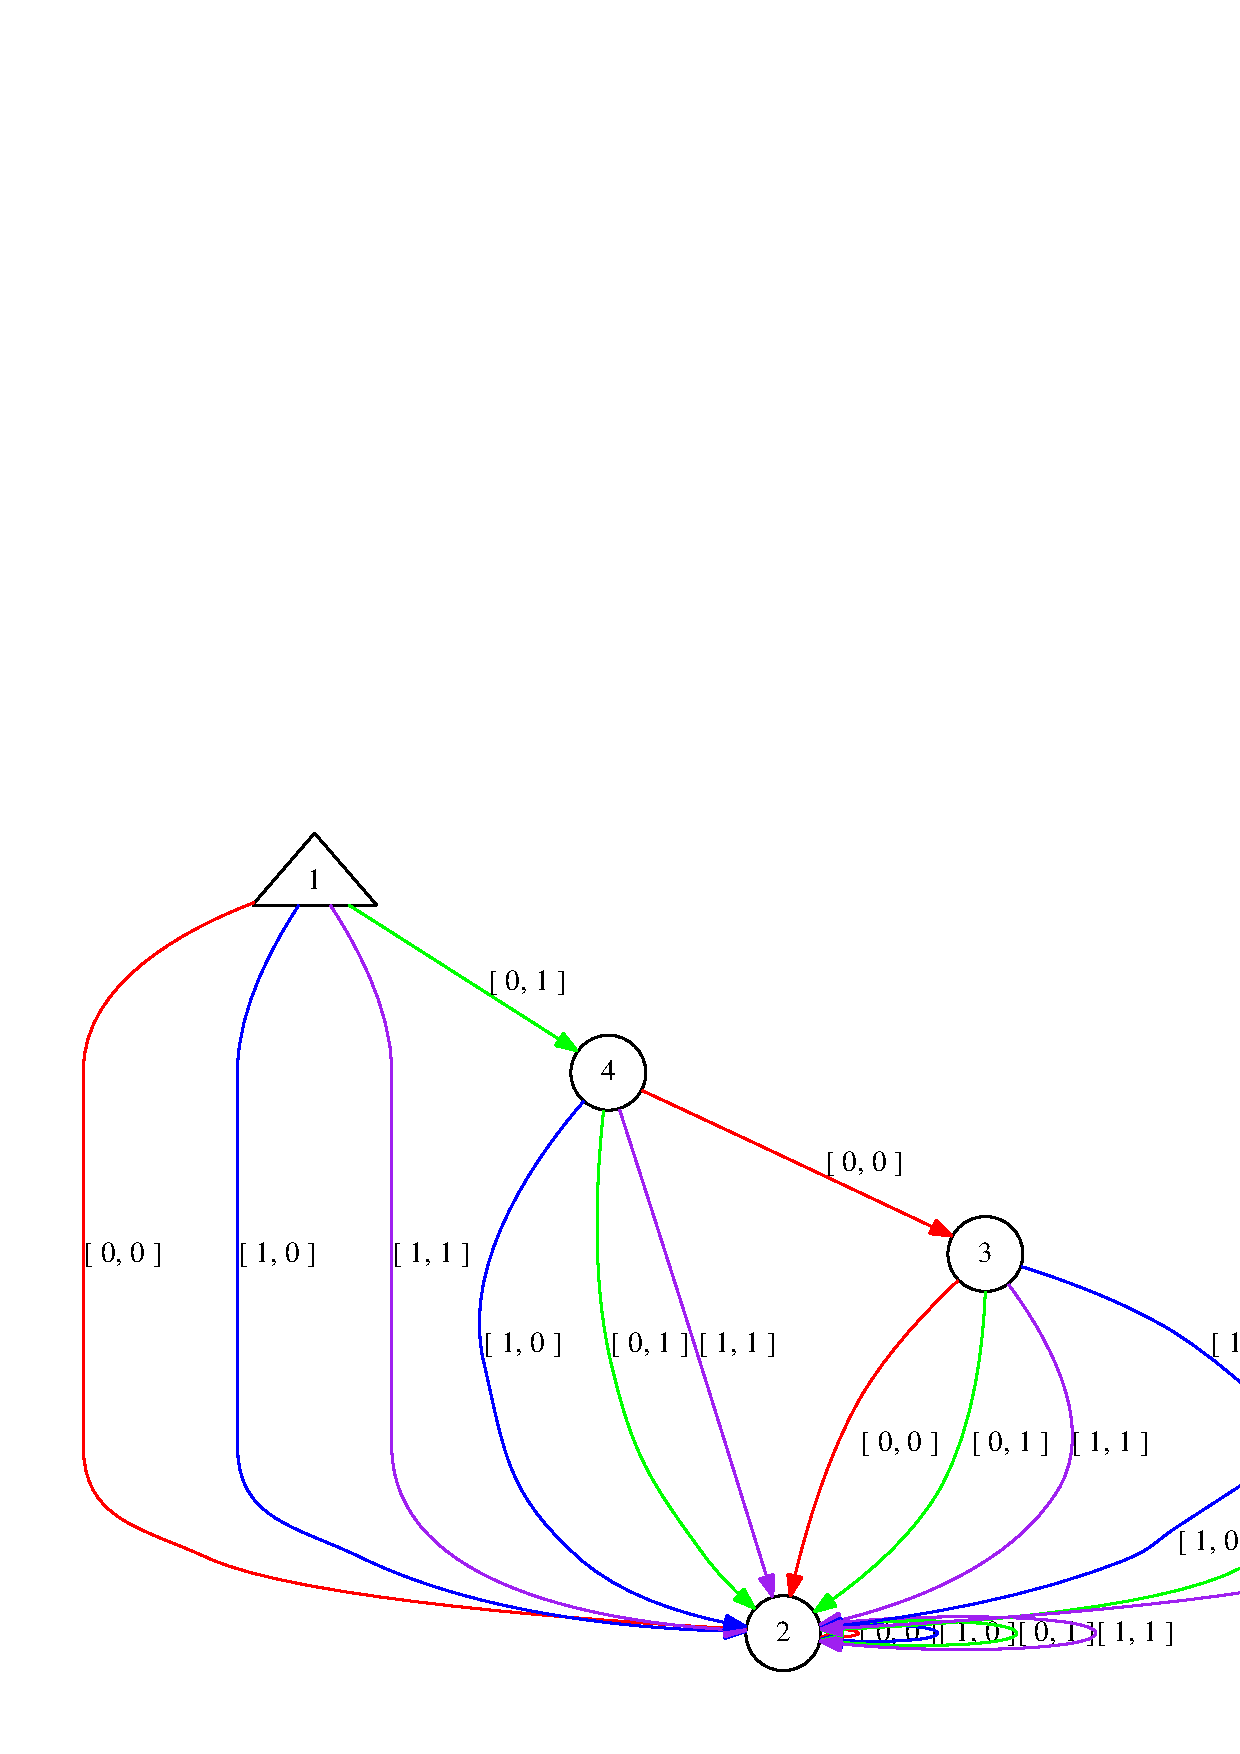
\includegraphics[width=0.8\textwidth]{img/ex1.jpg}
	\caption{A minimal DFA recognizing $x=4$ ($x$ corresponding to the first component of each letter) and $y=1$ ($y$ corresponding to the second component).}
	\label{ex1}
\end{figure}
  }

 
\subsection{\textcolor{Chapter }{Example 2: Recalling the motivation}}\logpage{[ 4, 2, 2 ]}
\hyperdef{L}{X83EF257286DFEB48}{}
{
 We recall the example from the section \ref{Introduction}. There we wanted to get the \texttt{Predicaton} recognizing all natural numbers which can be purchased by 6, 9 and 20. 
\begin{Verbatim}[commandchars=!@H,fontsize=\small,frame=single,label=Example]
  !gapprompt@gap>H !gapinput@# We create the Predicaton of the following formulaH
  !gapprompt@gap>H !gapinput@A:=Predicaton("(E x:(E y:(E z:6*x+9*y+20*z=n)))");H
  Predicaton: deterministic finite automaton on 2 letters with 17 states,
   the variable position list [ 1 ] and the following transitions:
           |  1  2  3  4  5  6  7  8  9  10 11 12 13 14 15 16 17 
  ---------------------------------------------------------------
    [ 0 ]  |  17 12 6  3  5  5  6  4  7  6  5  10 13 13 14 15 16 
    [ 1 ]  |  2  9  13 5  13 5  3  15 10 14 14 4  13 5  5  11 8  
   Initial states: [ 1 ]
   Final states:   [ 1, 13, 14, 15, 16, 17 ]
  
   The alphabet corresponds to the following variable list: [ "n" ].
  
   Output:
  < Predicaton: deterministic finite automaton on 2 letters with 17 states
  and the variable position list [ 1 ]. >
  !gapprompt@gap>H !gapinput@Display(A);H
  Predicaton: deterministic finite automaton on 2 letters with 17 states,
   the variable position list [ 1 ] and the following transitions:
           |  1  2  3  4  5  6  7  8  9  10 11 12 13 14 15 16 17 
  ---------------------------------------------------------------
    [ 0 ]  |  17 12 6  3  5  5  6  4  7  6  5  10 13 13 14 15 16 
    [ 1 ]  |  2  9  13 5  13 5  3  15 10 14 14 4  13 5  5  11 8  
   Initial states: [ 1 ]
   Final states:   [ 1, 13, 14, 15, 16, 17 ]
  
   The alphabet corresponds to the following variable list: [ "n" ].
  !gapprompt@gap>H !gapinput@# We ask for the accepted natural numbers.H
  !gapprompt@gap>H !gapinput@AcceptedByPredicaton(A, 20);H
  [ [ 0 ], [ 6 ], [ 9 ], [ 12 ], [ 15 ], [ 18 ], [ 20 ] ]
  !gapprompt@gap>H !gapinput@DisplayAcceptedByPredicaton(A, 99, true);H
   If the following words are accepted by the given automaton, then: Y,
   otherwise if not accepted: n.
     0: Y   1: n   2: n   3: n   4: n   5: n   6: Y   7: n   8: n   9: Y
    10: n  11: n  12: Y  13: n  14: n  15: Y  16: n  17: n  18: Y  19: n
    20: Y  21: Y  22: n  23: n  24: Y  25: n  26: Y  27: Y  28: n  29: Y
    30: Y  31: n  32: Y  33: Y  34: n  35: Y  36: Y  37: n  38: Y  39: Y
    40: Y  41: Y  42: Y  43: n  44: Y  45: Y  46: Y  47: Y  48: Y  49: Y
    50: Y  51: Y  52: Y  53: Y  54: Y  55: Y  56: Y  57: Y  58: Y  59: Y
    60: Y  61: Y  62: Y  63: Y  64: Y  65: Y  66: Y  67: Y  68: Y  69: Y
    70: Y  71: Y  72: Y  73: Y  74: Y  75: Y  76: Y  77: Y  78: Y  79: Y
    80: Y  81: Y  82: Y  83: Y  84: Y  85: Y  86: Y  87: Y  88: Y  89: Y
    90: Y  91: Y  92: Y  93: Y  94: Y  95: Y  96: Y  97: Y  98: Y  99: Y
   
  !gapprompt@gap>H !gapinput@# We create the Predicaton accepting the greatest non-accepted number.H
  !gapprompt@gap>H !gapinput@# First we create a PredicatonRepresentation, containing a name,H
  !gapprompt@gap>H !gapinput@# an arity and an automaton (the input may also be a Predicaton).H
  !gapprompt@gap>H !gapinput@p:=PredicatonRepresentation("P", 1, A);H
  < Predicaton represented with the name "P", the arity 1 and 
  the deterministic automaton on 2 letters and 17 states. >
  !gapprompt@gap>H !gapinput@AddToPredicataList(p);H
  !gapprompt@gap>H !gapinput@PredicataList;H
  < PredicataRepresentation containing the following predicates: [ "P" ]. >
  !gapprompt@gap>H !gapinput@B:=Predicaton("(A m: m > n implies P[m]) and not P[n]");H
  Predicaton: deterministic finite automaton on 2 letters with 8 states, 
  the variable position list [ 1 ] and the following transitions:
           |  1  2  3  4  5  6  7  8  
  ------------------------------------
    [ 0 ]  |  2  2  2  3  2  5  2  8  
    [ 1 ]  |  7  2  8  2  4  2  6  2  
   Initial states: [ 1 ]
   Final states:   [ 8 ]
  
   The alphabet corresponds to the following variable list: [ "n" ].
  
   Regular expression of the automaton:
     [ 1 ][ 1 ][ 0 ][ 1 ][ 0 ][ 1 ][ 0 ]*
  
   Output:
  < Predicaton: deterministic finite automaton on 2 letters with 8 states 
  and the variable position list [ 1 ]. >
  !gapprompt@gap>H !gapinput@AcceptedByPredicaton(B, 50);H
  [ [ 43 ] ]
  !gapprompt@gap>H !gapinput@# We look at the regular expression and compute the natural numberH
  !gapprompt@gap>H !gapinput@PredicatonToRatExp(B);H
  [ 1 ][ 1 ][ 0 ][ 1 ][ 0 ][ 1 ][ 0 ]*
  !gapprompt@gap>H !gapinput@BinToDec([ 1, 1, 0, 1, 0, 1 ]);H
  43
  !gapprompt@gap>H !gapinput@# Alternatively, we can also use the inbuilt function:H
  !gapprompt@gap>H !gapinput@C:=GreatestNonAcceptedNumber(A);H
  Predicaton: deterministic finite automaton on 2 letters with 8 states, 
  the variable position list [ 1 ] and the following transitions:
           |  1  2  3  4  5  6  7  8  
  ------------------------------------
    [ 0 ]  |  2  2  2  3  2  5  2  8  
    [ 1 ]  |  7  2  8  2  4  2  6  2  
   Initial states: [ 1 ]
   Final states:   [ 8 ]
  
   The alphabet corresponds to the following variable list: [ "n" ].
  
   Regular expression of the automaton:
     [ 1 ][ 1 ][ 0 ][ 1 ][ 0 ][ 1 ][ 0 ]*
  
   Output:
  < Predicaton: deterministic finite automaton on 2 letters with 8 states 
  and the variable position list [ 1 ]. >
\end{Verbatim}
 
\begin{figure}[ht]
	\centering
  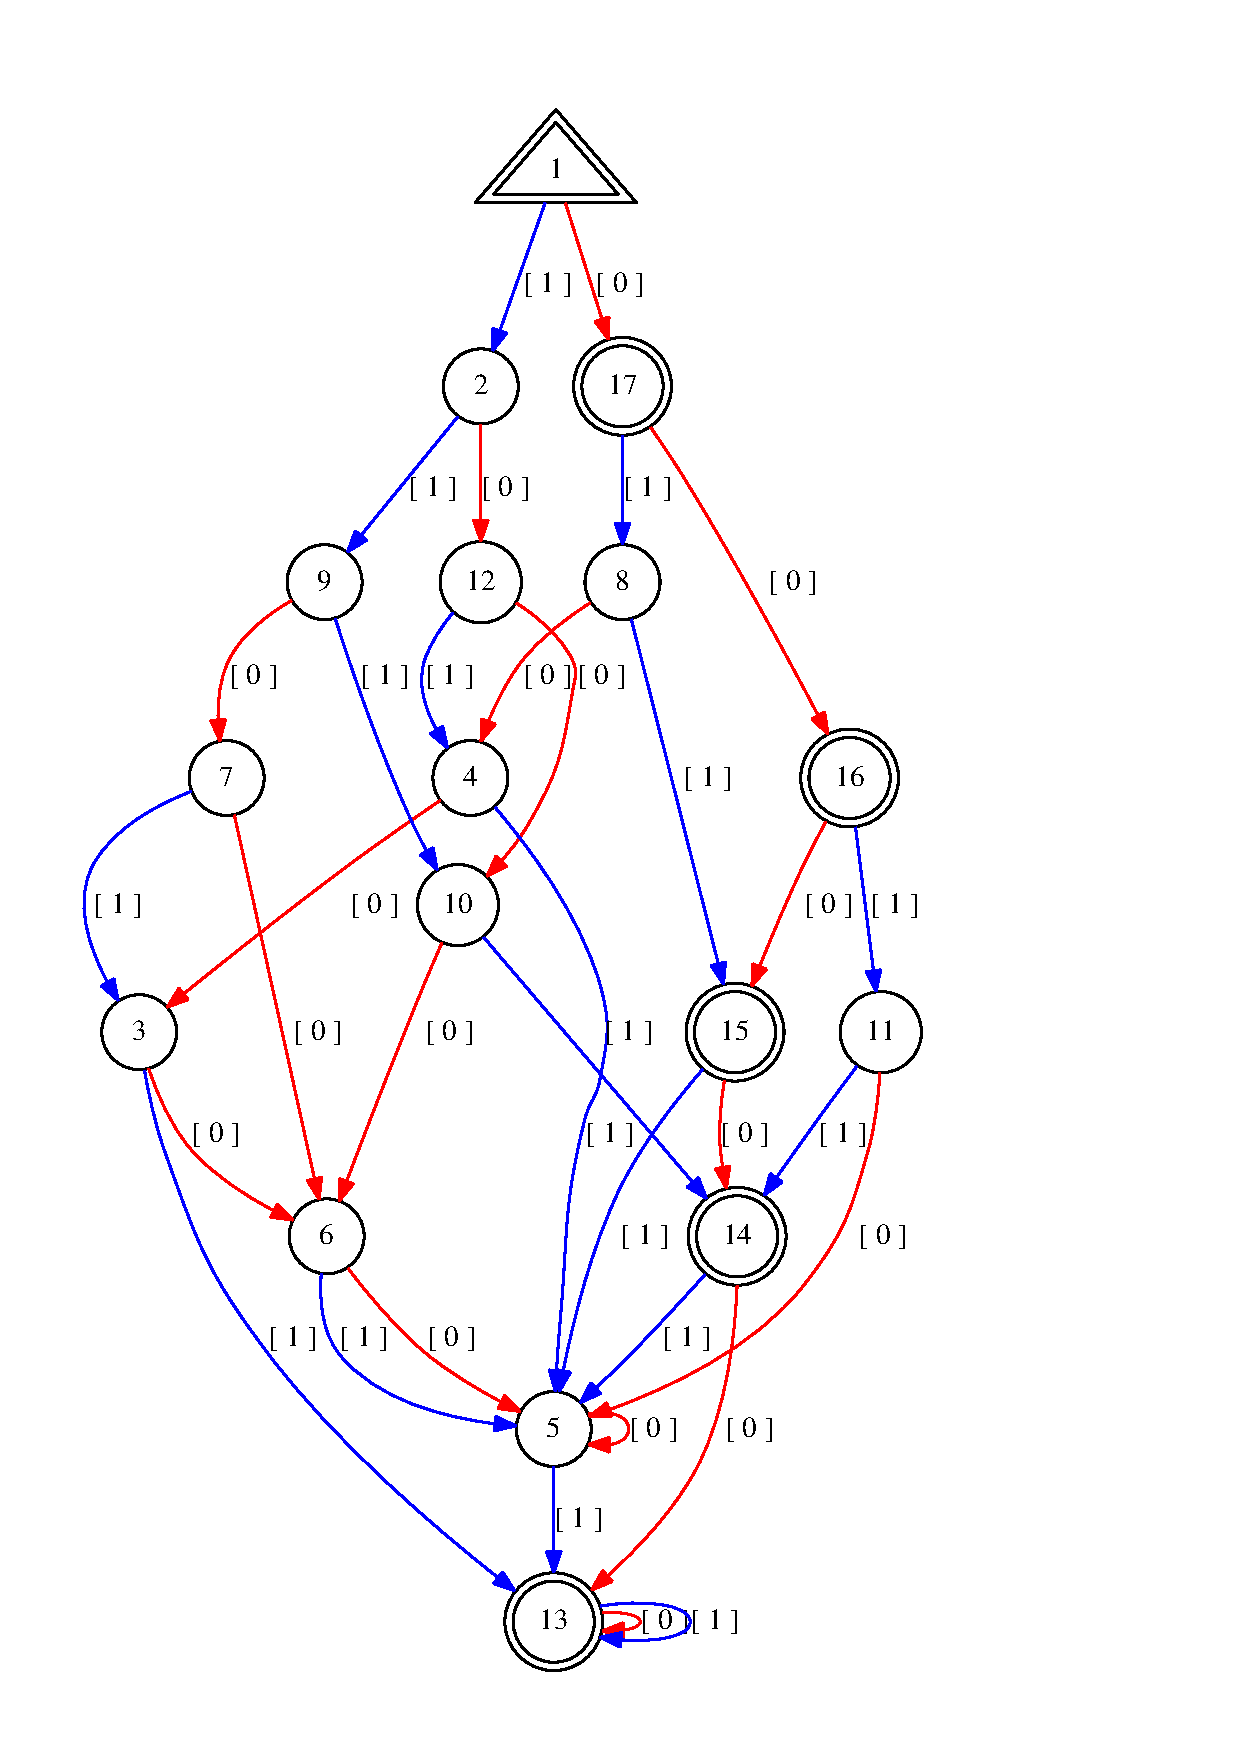
\includegraphics[width=0.5\textwidth]{img/aut1.jpg}
	\caption{A minimal DFA recognizing the numbers which can be purchased by the formula of \texttt{A}.}
	\label{ex5}
\end{figure}
\newpage
  }

 
\subsection{\textcolor{Chapter }{Example 3: Divisible by three}}\logpage{[ 4, 2, 3 ]}
\hyperdef{L}{X7AB61BD37A356EC4}{}
{
 A very common example from an automata theory lecture is finding the natural
numbers which are divisible by three. Sometimes this example is solve with
clear rules, sometimes with a lot of handwaving.

 However, the following way is a solid approach in the first-order language
with $+$ using the shortcut \texttt{3*x:=x+x+x}. 

 Here, first the \texttt{Predicaton} for \texttt{3*y=x} is created with the transition rule with the \texttt{k}-th state having carry \texttt{(k-1)}: \texttt{3*a[1]=a[2]+(i-1)+2*((j-1)-(i-1))}. For the existence quantifier we ignore the second component of each letter,
which yields a nondeterministic finite automaton. We apply the leading zero
completion (see \texttt{NormalizedLeadingZeroPredicaton} (\ref{NormalizedLeadingZeroPredicaton})), i.e. any leading zero may be cancelled or added to the accepted words. Then
we apply the subset construction and return the minimal automaton. 
\begin{Verbatim}[commandchars=!@G,fontsize=\small,frame=single,label=Example]
  !gapprompt@gap>G !gapinput@# We ask if there exists "y" s.t. 3*y=x.G
  !gapprompt@gap>G !gapinput@A:=Predicaton("(E y: 3*y = x)");G
  Predicaton: deterministic finite automaton on 2 letters with 3 states, 
  the variable position list [ 1 ] and the following transitions:
           |  1  2  3  
  ---------------------
    [ 0 ]  |  1  3  2  
    [ 1 ]  |  2  1  3  
   Initial states: [ 1 ]
   Final states:   [ 1 ]
  
   The alphabet corresponds to the following variable list: [ "x" ].
  
   Regular expression of the automaton:
     ([ 1 ]([ 0 ][ 1 ]*[ 0 ])*[ 1 ]U[ 0 ])*
  
   Output:
  < Predicaton: deterministic finite automaton on 2 letters with 3 states 
  and the variable position list [ 1 ]. >
  !gapprompt@gap>G !gapinput@# Compare with:G
  !gapprompt@gap>G !gapinput@B:=Predicaton("3*y = x");G
  Predicaton: deterministic finite automaton on 4 letters with 4 states, 
  the variable position list [ 1, 2 ] and the following transitions:
              |  1  2  3  4  
  ---------------------------
    [ 0, 0 ]  |  1  2  2  3  
    [ 1, 0 ]  |  2  2  1  2  
    [ 0, 1 ]  |  2  2  4  2  
    [ 1, 1 ]  |  3  2  2  4  
   Initial states: [ 1 ]
   Final states:   [ 1 ]
  
   The alphabet corresponds to the following variable list: [ "x", "y" ].
  
   Regular expression of the automaton:
     ([ 1, 1 ]([ 0, 1 ][ 1, 1 ]*[ 0, 0 ])*[ 1, 0 ]U[ 0, 0 ])*
  
   Output:
  < Predicaton: deterministic finite automaton on 4 letters with 4 states 
  and the variable position list [ 1, 2 ]. >
  !gapprompt@gap>G !gapinput@Display(B);G
  Predicaton: deterministic finite automaton on 4 letters with 4 states, 
  the variable position list [ 1, 2 ] and the following transitions:
              |  1  2  3  4  
  ---------------------------
    [ 0, 0 ]  |  1  2  2  3  
    [ 1, 0 ]  |  2  2  1  2  
    [ 0, 1 ]  |  2  2  4  2  
    [ 1, 1 ]  |  3  2  2  4  
   Initial states: [ 1 ]
   Final states:   [ 1 ]
  
   The alphabet corresponds to the following variable list: [ "x", "y" ].
  !gapprompt@gap>G !gapinput@C:=ExistsPredicaton(B, "y");;G
  !gapprompt@gap>G !gapinput@Display(C);G
  Predicaton: deterministic finite automaton on 2 letters with 3 states, 
  the variable position list [ 1 ] and the following transitions:
           |  1  2  3  
  ---------------------
    [ 0 ]  |  1  3  2  
    [ 1 ]  |  2  1  3  
   Initial states: [ 1 ]
   Final states:   [ 1 ]
  
   The alphabet corresponds to the following variable list: [ "x" ].
  !gapprompt@gap>G !gapinput@DrawPredicaton(A);G
\end{Verbatim}
 
\begin{figure}[ht]
	\centering
  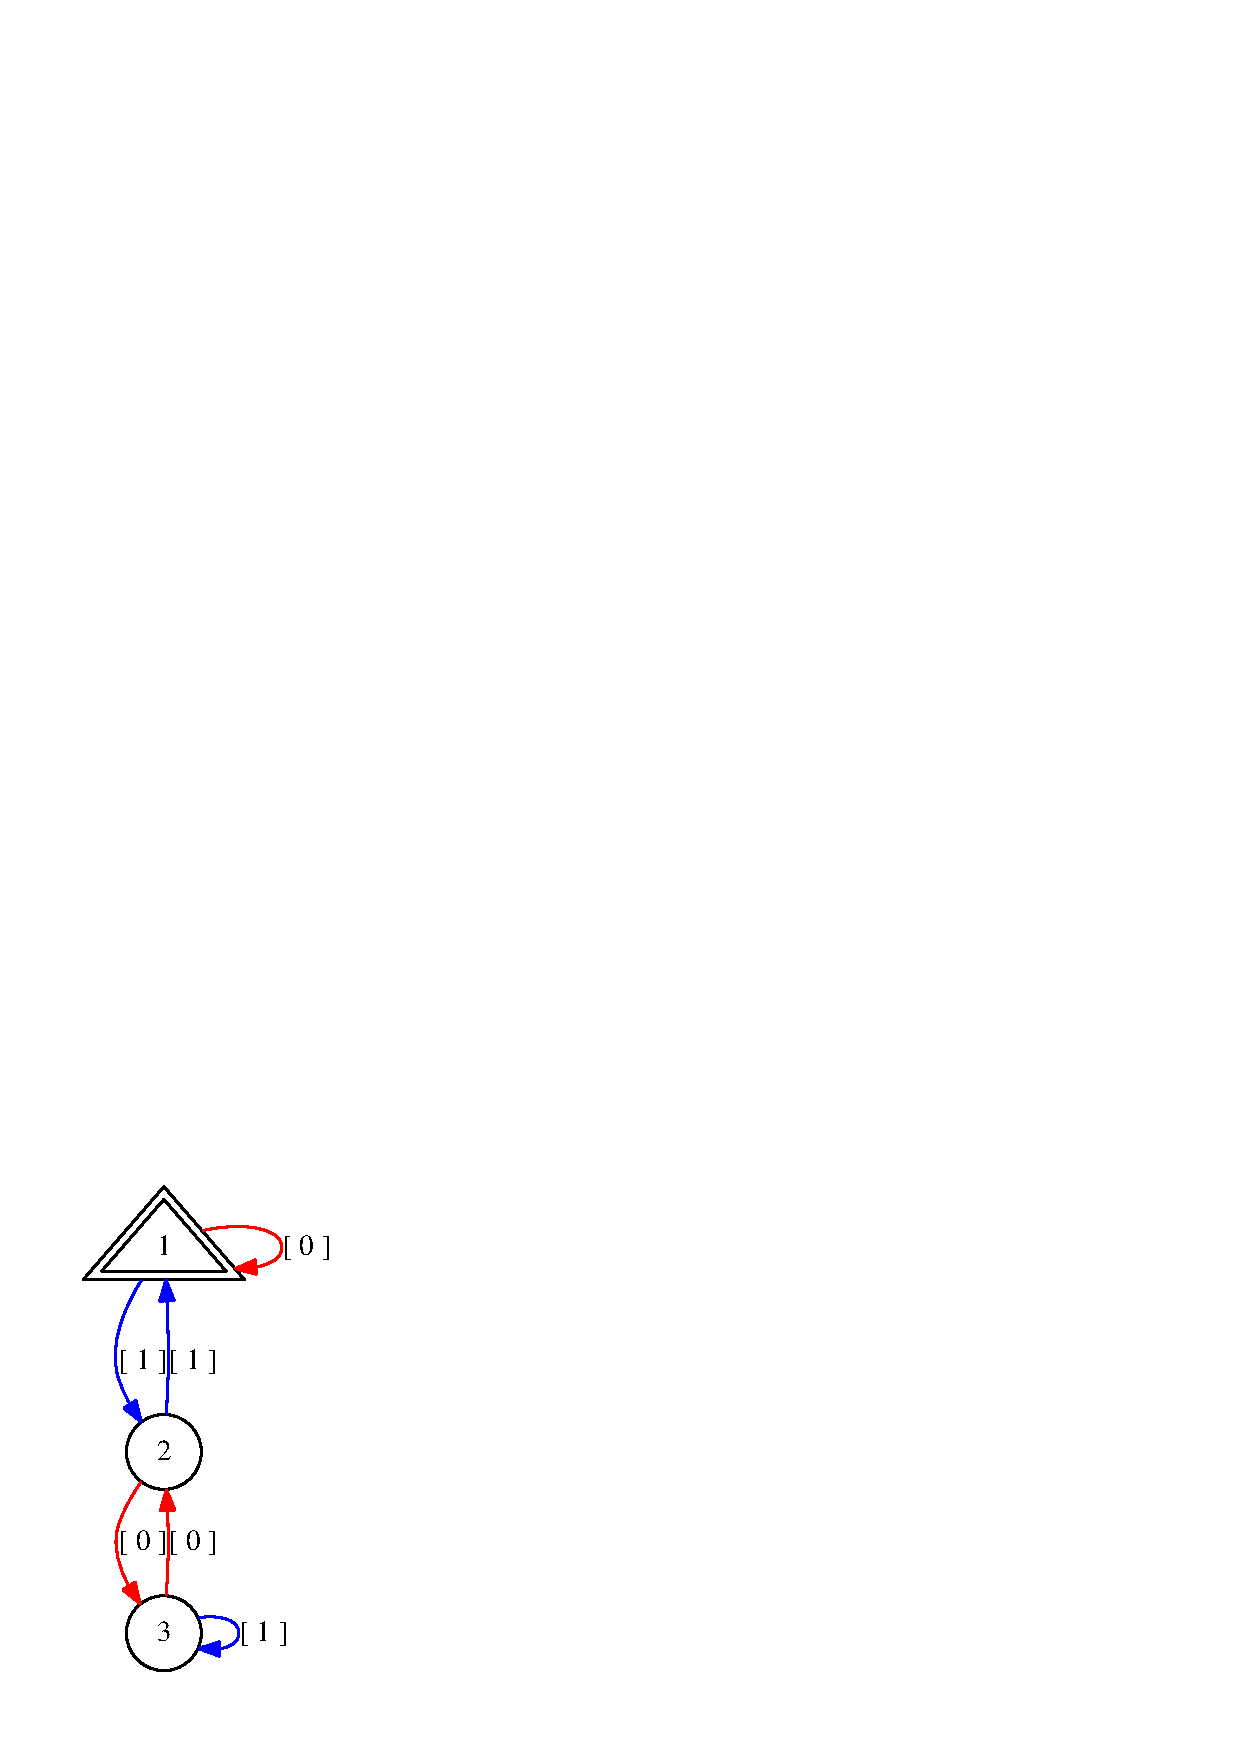
\includegraphics[width=0.2\textwidth]{img/ex3.jpg}
	\caption{A minimal DFA recognizing the numbers divisible by 3.}
	\label{ex3}
\end{figure}
  }

 
\subsection{\textcolor{Chapter }{Example 4: Linear congruences}}\logpage{[ 4, 2, 4 ]}
\hyperdef{L}{X818A9B737F7D6F27}{}
{
 We can solve the linear congruences $4\cdot x=7$ modulo 5 in the natural numbers. 
\begin{Verbatim}[commandchars=!@G,fontsize=\small,frame=single,label=Example]
  !gapprompt@gap>G !gapinput@A:=Predicaton("(E y: 4*x = 7+5*y)");G
  Predicaton: deterministic finite automaton on 2 letters with 5 states, 
  the variable position list [ 1 ] and the following transitions:
           |  1  2  3  4  5  
  ---------------------------
    [ 0 ]  |  4  1  2  3  5  
    [ 1 ]  |  2  5  1  4  3  
   Initial states: [ 1 ]
   Final states:   [ 5 ]
  
   The alphabet corresponds to the following variable list: [ "x" ].
  
   Output:
  < Predicaton: deterministic finite automaton on 2 letters with 5 states
  and the variable position list [ 1 ]. >
  !gapprompt@gap>G !gapinput@AcceptedByPredicaton(A, 20);G
  [ [ 3 ], [ 8 ], [ 13 ], [ 18 ] ]
  !gapprompt@gap>G !gapinput@# We asked for some accepted words and suggest as a solution x = 3+5*k.G
  !gapprompt@gap>G !gapinput@B:=Predicaton("(E k: x = 3+5*k)");G
  Predicaton: deterministic finite automaton on 2 letters with 5 states, 
  the variable position list [ 1 ] and the following transitions:
           |  1  2  3  4  5  
  ---------------------------
    [ 0 ]  |  4  1  2  3  5  
    [ 1 ]  |  2  5  1  4  3  
   Initial states: [ 1 ]
   Final states:   [ 5 ]
  
   The alphabet corresponds to the following variable list: [ "x" ].
  
   Output:
  < Predicaton: deterministic finite automaton on 2 letters with 5 states 
  and the variable position list [ 1 ]. >
  !gapprompt@gap>G !gapinput@# Indeed:G
  !gapprompt@gap>G !gapinput@AreEquivalentPredicata(A, B);G
  The Predicaton holds for all natural numbers and is interpreted as True.
  true
  !gapprompt@gap>G !gapinput@DrawPredicaton(A);G
  !gapprompt@gap>G !gapinput@# Furthermore, we look at a system of linear congruences.G
  !gapprompt@gap>G !gapinput@C:=Predicaton("(E y1: x = 1 + 2*y1) and (E y2: x = 2 + 3*y2)");G
  Predicaton: deterministic finite automaton on 2 letters with 5 states, 
  the variable position list [ 1 ] and the following transitions:
           |  1  2  3  4  5  
  ---------------------------
    [ 0 ]  |  2  2  4  3  5  
    [ 1 ]  |  4  2  5  4  3  
   Initial states: [ 1 ]
   Final states:   [ 5 ]
  
   The alphabet corresponds to the following variable list: [ "x" ].
  
   Regular expression of the automaton:
     [ 1 ][ 1 ]*[ 0 ]([ 1 ][ 0 ]*[ 1 ]U[ 0 ][ 1 ]*[ 0 ])*[ 1 ][ 0 ]*
  
   Output:
  < Predicaton: deterministic finite automaton on 2 letters with 5 states 
  and the variable position list [ 1 ]. >
  !gapprompt@gap>G !gapinput@AcceptedByPredicaton(C, 20);G
  [ [ 5 ], [ 11 ], [ 17 ] ]
  !gapprompt@gap>G !gapinput@# We suggest:G
  !gapprompt@gap>G !gapinput@D:=Predicaton("(E k: x = 5 + 6 * k)");G
  Predicaton: deterministic finite automaton on 2 letters with 5 states, 
  the variable position list [ 1 ] and the following transitions:
           |  1  2  3  4  5  
  ---------------------------
    [ 0 ]  |  2  2  4  3  5  
    [ 1 ]  |  4  2  5  4  3  
   Initial states: [ 1 ]
   Final states:   [ 5 ]
  
   The alphabet corresponds to the following variable list: [ "x" ].
  
   Regular expression of the automaton:
     [ 1 ][ 1 ]*[ 0 ]([ 1 ][ 0 ]*[ 1 ]U[ 0 ][ 1 ]*[ 0 ])*[ 1 ][ 0 ]*
  
   Output:
  < Predicaton: deterministic finite automaton on 2 letters with 5 states 
  and the variable position list [ 1 ]. >
  !gapprompt@gap>G !gapinput@AreEquivalentPredicata(C, D);G
  The Predicaton holds for all natural numbers and is interpreted as True.
  true
\end{Verbatim}
 
\begin{figure}[ht]
	\centering
  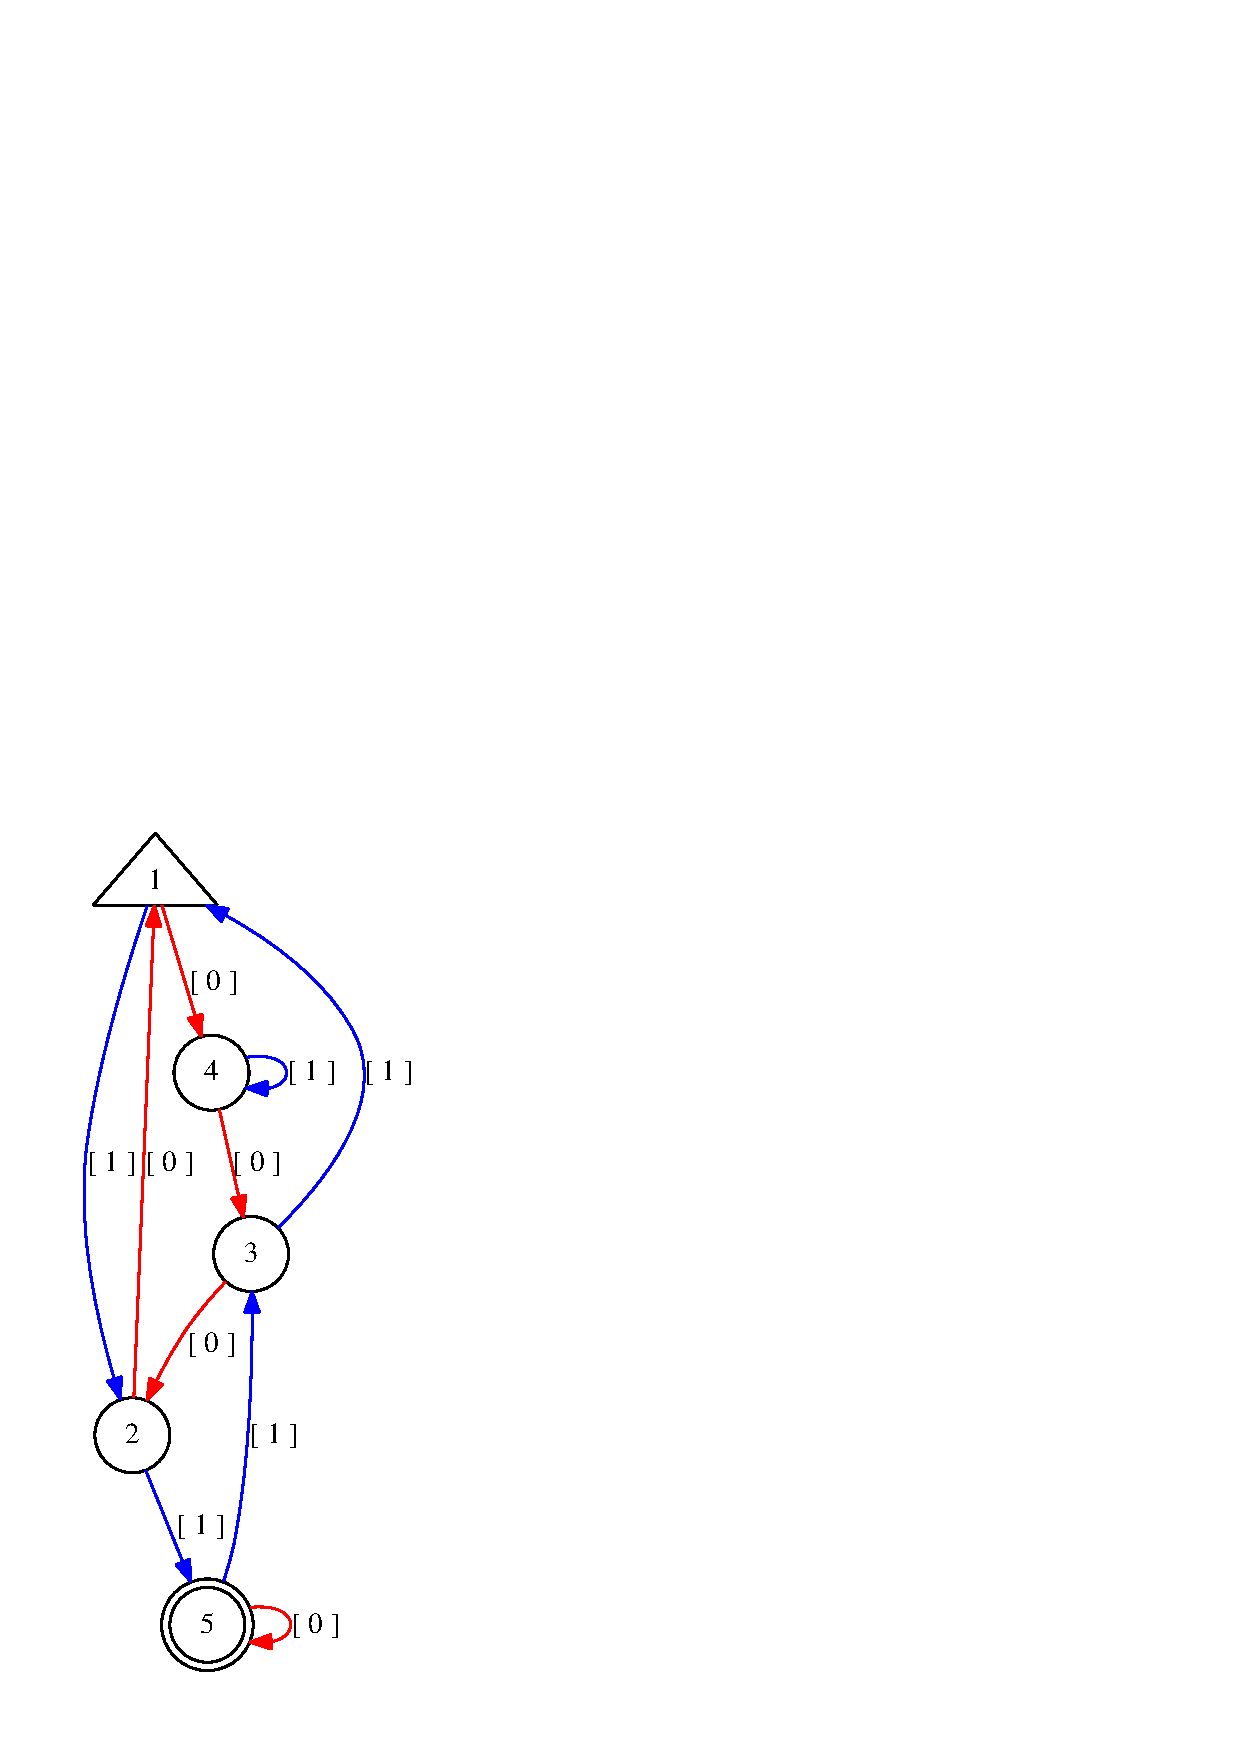
\includegraphics[width=0.25\textwidth]{img/ex4.jpg}
	\caption{A minimal DFA recognizing the solutions of the linear congruence \texttt{A}.}
	\label{ex4}
\end{figure}
  }

 
\subsection{\textcolor{Chapter }{Example 5: GCD and LCM}}\logpage{[ 4, 2, 5 ]}
\hyperdef{L}{X860922F3860BAE43}{}
{
 We can also compute the GCD and LCM of two natural numbers, however at the
first sight it's not completely obvious how to obtain the GCD. 
\begin{Verbatim}[commandchars=!@H,fontsize=\small,frame=single,label=Example]
  !gapprompt@gap>H !gapinput@# All multiples of the GCD of 6 and 15. If there exists z such thatH
  !gapprompt@gap>H !gapinput@# it is a multiple of the GCD(6, 15) after some number y, then alsoH
  !gapprompt@gap>H !gapinput@# z+x is a multiple of the GCD.H
  !gapprompt@gap>H !gapinput@A:=Predicaton("(E y: (A z: z>=y implies ((Ea : (Eb: z= 6*a+15*b))\H
  !gapprompt@>H !gapinput@implies (Ec: (Ed: z+x= 6*c+15*d)))))");H
  
  Predicaton: deterministic finite automaton on 2 letters with 3 states, 
  the variable position list [ 1 ] and the following transitions:
           |  1  2  3  
  ---------------------
    [ 0 ]  |  1  3  2  
    [ 1 ]  |  2  1  3  
   Initial states: [ 1 ]
   Final states:   [ 1 ]
  
   The alphabet corresponds to the following variable list: [ "x" ].
  
   Regular expression of the automaton:
     ([ 1 ]([ 0 ][ 1 ]*[ 0 ])*[ 1 ]U[ 0 ])*
  
   Output:
  < Predicaton: deterministic finite automaton on 2 letters with 3 states 
  and the variable position list [ 1 ]. >
  !gapprompt@gap>H !gapinput@# This Predicaton is already known from Example 2 and we test for the leastH
  !gapprompt@gap>H !gapinput@# accepted natural number greater 0 (>= 0 with optional parameter false):H
  !gapprompt@gap>H !gapinput@B:=LeastAcceptedNumber(A);H
  Predicaton: deterministic finite automaton on 2 letters with 4 states, 
  the variable position list [ 1 ] and the following transitions:
           |  1  2  3  4  
  ------------------------
    [ 0 ]  |  2  2  2  4  
    [ 1 ]  |  3  2  4  2  
   Initial states: [ 1 ]
   Final states:   [ 4 ]
  
   The alphabet corresponds to the following variable list: [ "x" ].
  
   Regular expression of the automaton:
     [ 1 ][ 1 ][ 0 ]*
  
   Output:
  < Predicaton: deterministic finite automaton on 2 letters with 4 states 
  and the variable position list [ 1 ]. >
  !gapprompt@gap>H !gapinput@AcceptedByPredicaton(B);H
  [ [ 3 ] ]
  !gapprompt@gap>H !gapinput@# We get the multiples of the LCM(6, 15) straightforwardly.H
  !gapprompt@gap>H !gapinput@C:=Predicaton("(E a: 6*a = x) and (E b: 15*b = x)");H
  Predicaton: deterministic finite automaton on 2 letters with 17 states, 
  the variable position list [ 1 ] and the following transitions:
           |  1  2  3  4  5  6  7  8  9  10 11 12 13 14 15 16 17 
  ---------------------------------------------------------------
    [ 0 ]  |  17 2  6  3  4  5  10 7  8  9  12 11 16 13 14 15 17 
    [ 1 ]  |  2  2  17 6  7  13 5  3  11 16 10 4  12 8  15 9  14 
   Initial states: [ 1 ]
   Final states:   [ 1, 17 ]
  
   The alphabet corresponds to the following variable list: [ "x" ].
  
   Output:
  < Predicaton: deterministic finite automaton on 2 letters with 17 states 
  and the variable position list [ 1 ]. >
  !gapprompt@gap>H !gapinput@D:=LeastAcceptedNumber(C);H
  Predicaton: deterministic finite automaton on 2 letters with 7 states, 
  the variable position list [ 1 ] and the following transitions:
           |  1  2  3  4  5  6  7  
  ---------------------------------
    [ 0 ]  |  6  2  2  2  2  2  7  
    [ 1 ]  |  2  2  7  3  4  5  2  
   Initial states: [ 1 ]
   Final states:   [ 7 ]
  
   The alphabet corresponds to the following variable list: [ "x" ].
  
   Regular expression of the automaton:
     [ 0 ][ 1 ][ 1 ][ 1 ][ 1 ][ 0 ]*
  
   Output:
  < Predicaton: deterministic finite automaton on 2 letters with 7 states 
  and the variable position list [ 1 ]. >
  !gapprompt@gap>H !gapinput@AcceptedByPredicaton(D, 100);H
  [ [ 30 ] ]
\end{Verbatim}
 }

 
\subsection{\textcolor{Chapter }{Example 6: Theorems}}\logpage{[ 4, 2, 6 ]}
\hyperdef{L}{X85C3C1597E55C80C}{}
{
 
\begin{Verbatim}[commandchars=!@B,fontsize=\small,frame=single,label=Example]
  !gapprompt@gap>B !gapinput@# Which of the followings sentences are true?B
  !gapprompt@gap>B !gapinput@A1:=Predicaton("(E x:(A y: x = y))");B
  Predicaton: deterministic finite automaton on 1 letter with 1 state, 
  the variable position list [ ] and the following transitions:
         |  1  
  -------------
    [ ]  |  1  
   Initial states: [ 1 ]
   Final states:   [ ]
  
   Regular expression of the automaton:
     empty_set
  
   Due to the automaton the formula is false.
     false
  
   Output:
  < Predicaton: deterministic finite automaton on 1 letter with 1 state 
  and the variable position list [ ]. >
  !gapprompt@gap>B !gapinput@A2:=Predicaton("(A x:(E y: x = y))");B
  Predicaton: deterministic finite automaton on 1 letter with 1 state, 
  the variable position list [ ] and the following transitions:
         |  1  
  -------------
    [ ]  |  1  
   Initial states: [ 1 ]
   Final states:   [ 1 ]
  
   Regular expression of the automaton:
     [ ]*
  
   Due to the automaton the formula is true.
     true
  
   Output:
  < Predicaton: deterministic finite automaton on 1 letter with 1 state 
  and the variable position list [ ]. >
  !gapprompt@gap>B !gapinput@A3:=Predicaton("(A x:(E y: x = y+1))");B
  Predicaton: deterministic finite automaton on 1 letter with 1 state, 
  the variable position list [ ] and the following transitions:
         |  1  
  -------------
    [ ]  |  1  
   Initial states: [ 1 ]
   Final states:   [ ]
  
   Regular expression of the automaton:
     empty_set
  
   Due to the automaton the formula is false.
     false
  
   Output:
  < Predicaton: deterministic finite automaton on 1 letter with 1 state 
  and the variable position list [ ]. >
  !gapprompt@gap>B !gapinput@A4:=Predicaton("(A x:(E y: x = 2*y) or (E y: x=2*y+1))");B
  Predicaton: deterministic finite automaton on 1 letter with 1 state, 
  the variable position list [ ] and the following transitions:
         |  1  
  -------------
    [ ]  |  1  
   Initial states: [ 1 ]
   Final states:   [ 1 ]
  
   Regular expression of the automaton:
     [ ]*
  
   Due to the automaton the formula is true.
     true
  
   Output:
  < Predicaton: deterministic finite automaton on 1 letter with 1 state 
  and the variable position list [ ]. >
  !gapprompt@gap>B !gapinput@A5:=Predicaton("(A n:(E n0: n > n0 implies (E x: (E y: 5*x+6*y=n))))");B
  Predicaton: deterministic finite automaton on 1 letter with 1 state, 
  the variable position list [ ] and the following transitions:
         |  1  
  -------------
    [ ]  |  1  
   Initial states: [ 1 ]
   Final states:   [ 1 ]
  
   Regular expression of the automaton:
     [ ]*
  
   Due to the automaton the formula is true.
     true
  
   Output:
  < Predicaton: deterministic finite automaton on 1 letter with 1 state 
  and the variable position list [ ]. >
  !gapprompt@gap>B !gapinput@# Furthermore, we can use "true" and "false" as predicates;B
  !gapprompt@gap>B !gapinput@A6:=Predicaton("true and (false implies true) implies true");B
  Predicaton: deterministic finite automaton on 1 letter with 1 state, 
  the variable position list [ ] and the following transitions:
         |  1  
  -------------
    [ ]  |  1  
   Initial states: [ 1 ]
   Final states:   [ 1 ]
  
   Regular expression of the automaton:
     [ ]*
  
   Due to the automaton the formula is true.
     true
  
   Output:
  < Predicaton: deterministic finite automaton on 1 letter with 1 state 
  and the variable position list [ ]. >
\end{Verbatim}
 
\begin{figure}[ht]
	\centering
  \includegraphics[width=0.2\textwidth]{img/ex6a.jpg}
	\caption{The minimal DFA which is interpreted as true.}
	\label{ex6a}
\end{figure}
  
\begin{figure}[ht]
	\centering
  \includegraphics[width=0.2\textwidth]{img/ex6b.jpg}
	\caption{The minimal DFA which is interpreted as false.}
	\label{ex6b}
\end{figure}
  }

 }

 }

 \def\bibname{References\logpage{[ "Bib", 0, 0 ]}
\hyperdef{L}{X7A6F98FD85F02BFE}{}
}

\bibliographystyle{alpha}
\bibliography{manualbib.xml}

\addcontentsline{toc}{chapter}{References}

\def\indexname{Index\logpage{[ "Ind", 0, 0 ]}
\hyperdef{L}{X83A0356F839C696F}{}
}

\cleardoublepage
\phantomsection
\addcontentsline{toc}{chapter}{Index}


\printindex

\newpage
\immediate\write\pagenrlog{["End"], \arabic{page}];}
\immediate\closeout\pagenrlog
\end{document}
